\documentclass[12pt,oneside, onecolumn,a4paper]{pharmmlspec}

% Need this to make some of the maths definitions work.
\DeclareMathOperator{\sech}{sech}
\DeclareMathOperator{\csch}{csch}
\DeclareMathOperator{\arcsec}{arcsec}
\DeclareMathOperator{\arccsc}{arccsc}
\DeclareMathOperator{\arccot}{arccot}
\DeclareMathOperator{\arcsinh}{arcsinh}
\DeclareMathOperator{\arccosh}{arccosh}
\DeclareMathOperator{\arctanh}{arctanh}
\DeclareMathOperator{\arcsech}{arcsech}
\DeclareMathOperator{\arccsch}{arccsch}
\DeclareMathOperator{\arccoth}{arccoth}

\newcounter{issuecntr}
\newenvironment{issues}{\begin{description}}{\end{description}}
%\newcommand*{\iss}[1]{\refstepcounter{issuecntr}\item[Issue \theissuecntr: #1]}
\newcommand*{\iss}[1]{\item[Issue: #1]}


%\includeonly{input/Scope}
%\includeonly{input/introduction_specSection}
%\includeonly{input/validation_rules}
%\includeonly{input/language_overview}
%\includeonly{input/explanatory_examples, input/bibliography}
%\includeonly{input/trialDesign_specSection, input/explanatory_examples, input/bibliography}
%\includeonly{input/mathDescription_specSection,  input/trialDesign_specSection}
%\includeonly{input/mathDescription_specSection, input/explanatory_examples, input/explanatory_examples_prt2}
%\includeonly{input/introduction_specSection, input/Scope, input/mathDescription_specSection, input/trialDesign_specSection}
%\includeonly{input/explanatory_examples, input/bibliography}
%\includeonly{input/explanatory_examples, input/explanatory_examples_prt2, input/bibliography}
%\includeonly{input/mathDescription_specSection, input/explanatory_examples, input/explanatory_examples_prt2, input/bibliography}
%\includeonly{input/trialDesign_specSection, input/explanatory_examples, input/explanatory_examples_prt2, input/bibliography}
%\includeonly{input/trialDesign_specSection,  input/language_overview, input/explanatory_examples, input/explanatory_examples_prt2, input/bibliography}


\thanksmarkseries{arabic}
\title{PharmML: The Pharmacometrics Markup Language\\
\vspace{1cm}
\Large%
Language Specification}
\author{Stuart L. Moodie\thanks{These authors contributed equally to the
  work}\thanks{EMBL-EBI, Hinxton, UK}, Maciej J. Swat\thanksmark{1}\thanksmark{2}\\
Niels R. Kristensen\thanks{Novo Nordisk A/S, Bagsv\ae rd, DK}
and Nicolas Le Nov\`{e}re\thanksmark{2}\thanks{Babraham Institute,
  Babraham, UK}}
\date{25 Sep 2013}
%\date{\today}

\setlength{\droptitle}{2cm}
\renewcommand{\maketitlehooka}{
\includegraphics{logos/ddmore_logo}\\
\vspace*{2cm}
\HRule
}
\renewcommand{\maketitlehookb}{\flushleft\Large%
\vspace*{1cm}
}

% \renewcommand{\maketitlehookd}{%
% \vspace*{4cm}
%  \flushleft%
%   \begin{minipage}{8cm}\color{DarkRed}\small
%   Disclaimer: This is a working draft of the PharmML specification. It is not a normative document.
% \end{minipage}
% }

\pretitle{%
\begin{flushleft}
\LARGE
}
\posttitle{%
\par
\vspace{0.5em}
\large
Version 0.2.1\\
\end{flushleft}%
\HRule
}
\preauthor{%
\begin{flushleft}
\large
}
\postauthor{%
\par
\end{flushleft}
}
\predate{%
\vspace{1cm}
\begin{flushleft}
\large
}
\postdate{%
\par
\end{flushleft}
}

%\usethanksrule
%\setlength{\thanksmarkwidth}{9cm}

\begin{document}

\frontmatter

%\renewcommand{\thefootnote}{\fnsymbol{footnote}}

\begin{titlingpage}
\usethanksrule
 \maketitle
\end{titlingpage}


\cleardoublepage

\vspace*{\stretch{1}}
   \begin{minipage}{16cm}%
Copyright \copyright\xspace 2013 The European Molecular Biology
Laboratory, Heidelberg, Germany\\* and Novo Nordisk A/S, Bagsv\ae rd, Denmark.
\end{minipage}

% \chapter*{Revision History}
% \begin{tabularx}{\linewidth}{ c  c  c  X }\toprule%
% \textbf{Version} & \textbf{Date} & \textbf{Author} & \textbf{Comments} \\ \midrule
% 0.1 & 22 Mar 2013 & All & First release for review.\\
% \bottomrule
% \end{tabularx}

\chapter*{Acknowledgements}

 \begin{quote}
{\small
When you know a thing, to hold that you know it; and when you do not know a thing, to allow that you do not know it - this is knowledge.\\
\textit{Confucius, The Confucian Analects}}
\end{quote}

In developing this latest version of \pharmml we are building on work
we documented in the previous version of this specification, the
contributions to which we acknowledged (see
section~\ref{chap:acknow-v0_1}). This latest version has been
developed over a shorter timeframe and during the summer vacation
period so consequently we are acknowledging a smaller number of
people. As ever we would like to acknowledge the input of Marc
Lavielle: the changes to the parameter and error model in this version
we were considerably influenced by his input. During the early stages
of development we sent out a proposal document, asking for feedback
and we are grateful to Mike Smith, Emmanuelle Comets, Duncan Edwards
and Marc Lavielle for the useful feedback they gave to these ideas. We
are also indebted to Paolo Magni for his work encoding models in the
previous version of \pharmml. In doing so he highlighted some
limitations in that version and helped spark some useful discussion
that helped us improved this version. Duncan Edwards also provided
excellent review comments to version 0.1.0 and the changes to the
changes we define data and represent the variability model are all
attributable to him. Roberto Bizzotto helped us to understand the
different flavours of the residual error models and their encoding in
MLXTRAN and NMTRAN. Since the last release there have been a number of
discussions on the DDMoRe WP4 mailing list and we would like to thank
the contributors (most of whom we mentioned already) include Andy
Hooker and Nick Holford. We would like to thank Nick in particular for
asking us to encode the model described by Chan \emph{et al.}\xspace
\cite{Chan:2005fk}. Together with Phylinda Chan, Nick helped us
understand what was a challenging trial design that gave us a great
test case to work on. Vincent Buchheit and his EFPIA colleagues
provided valuable feedback on different trial design aspects.  We
would like to thank Mihai Glont and Raza Ali for
scrutinising the specification during their work on the \ddmore
repository. Raza in particular provided some useful feedback on the
maths section in the language overview chapter. Sarah Keating helped
us understand the complexity of unit consistency checking and although
this feature is not in this version, we believe her experience will
help us get it right in the future.

We'd also like to thank Lutz Harnisch for his leadership of the
\ddmore project and the administrative team at Interface Europe for
their help ensuring its smooth running. Finally we would like to thank
Wendy Aartsen for many things, but specifically for organising the
April consortium meeting, which provided such an excellent forum for
the language specification.

The \ddmore project and consequently this work, is funded by the
Innovative Medicines Initiative (IMI), a large-scale public-private
partnership between the European Union and the pharmaceutical industry
association EFPIA\@. We would like to gratefully acknowledge their
support.



%%% Local Variables: 
%%% mode: latex
%%% TeX-master: "../pharmml-specification"
%%% End: 


\clearpage

\tableofcontents

%\clearpage

%\listoffigures

\mainmatter
\renewcommand{\thefootnote}{\arabic{footnote}}

\modulolinenumbers[5]
\linenumbers

\part{\pharmml Primer}
\label{part:primer}


% \chapter{What is \pharmml?}
\newcommand{\matlab}{MATLAB\textsuperscript{\textregistered}}
\chapter{What is \pharmml?}
\label{chap:pharmml-what}

\section{The Problem}

%\begin{figure}[h]
%{
%\centering
\begin{wrapfigure}{r}{0.45\linewidth}
  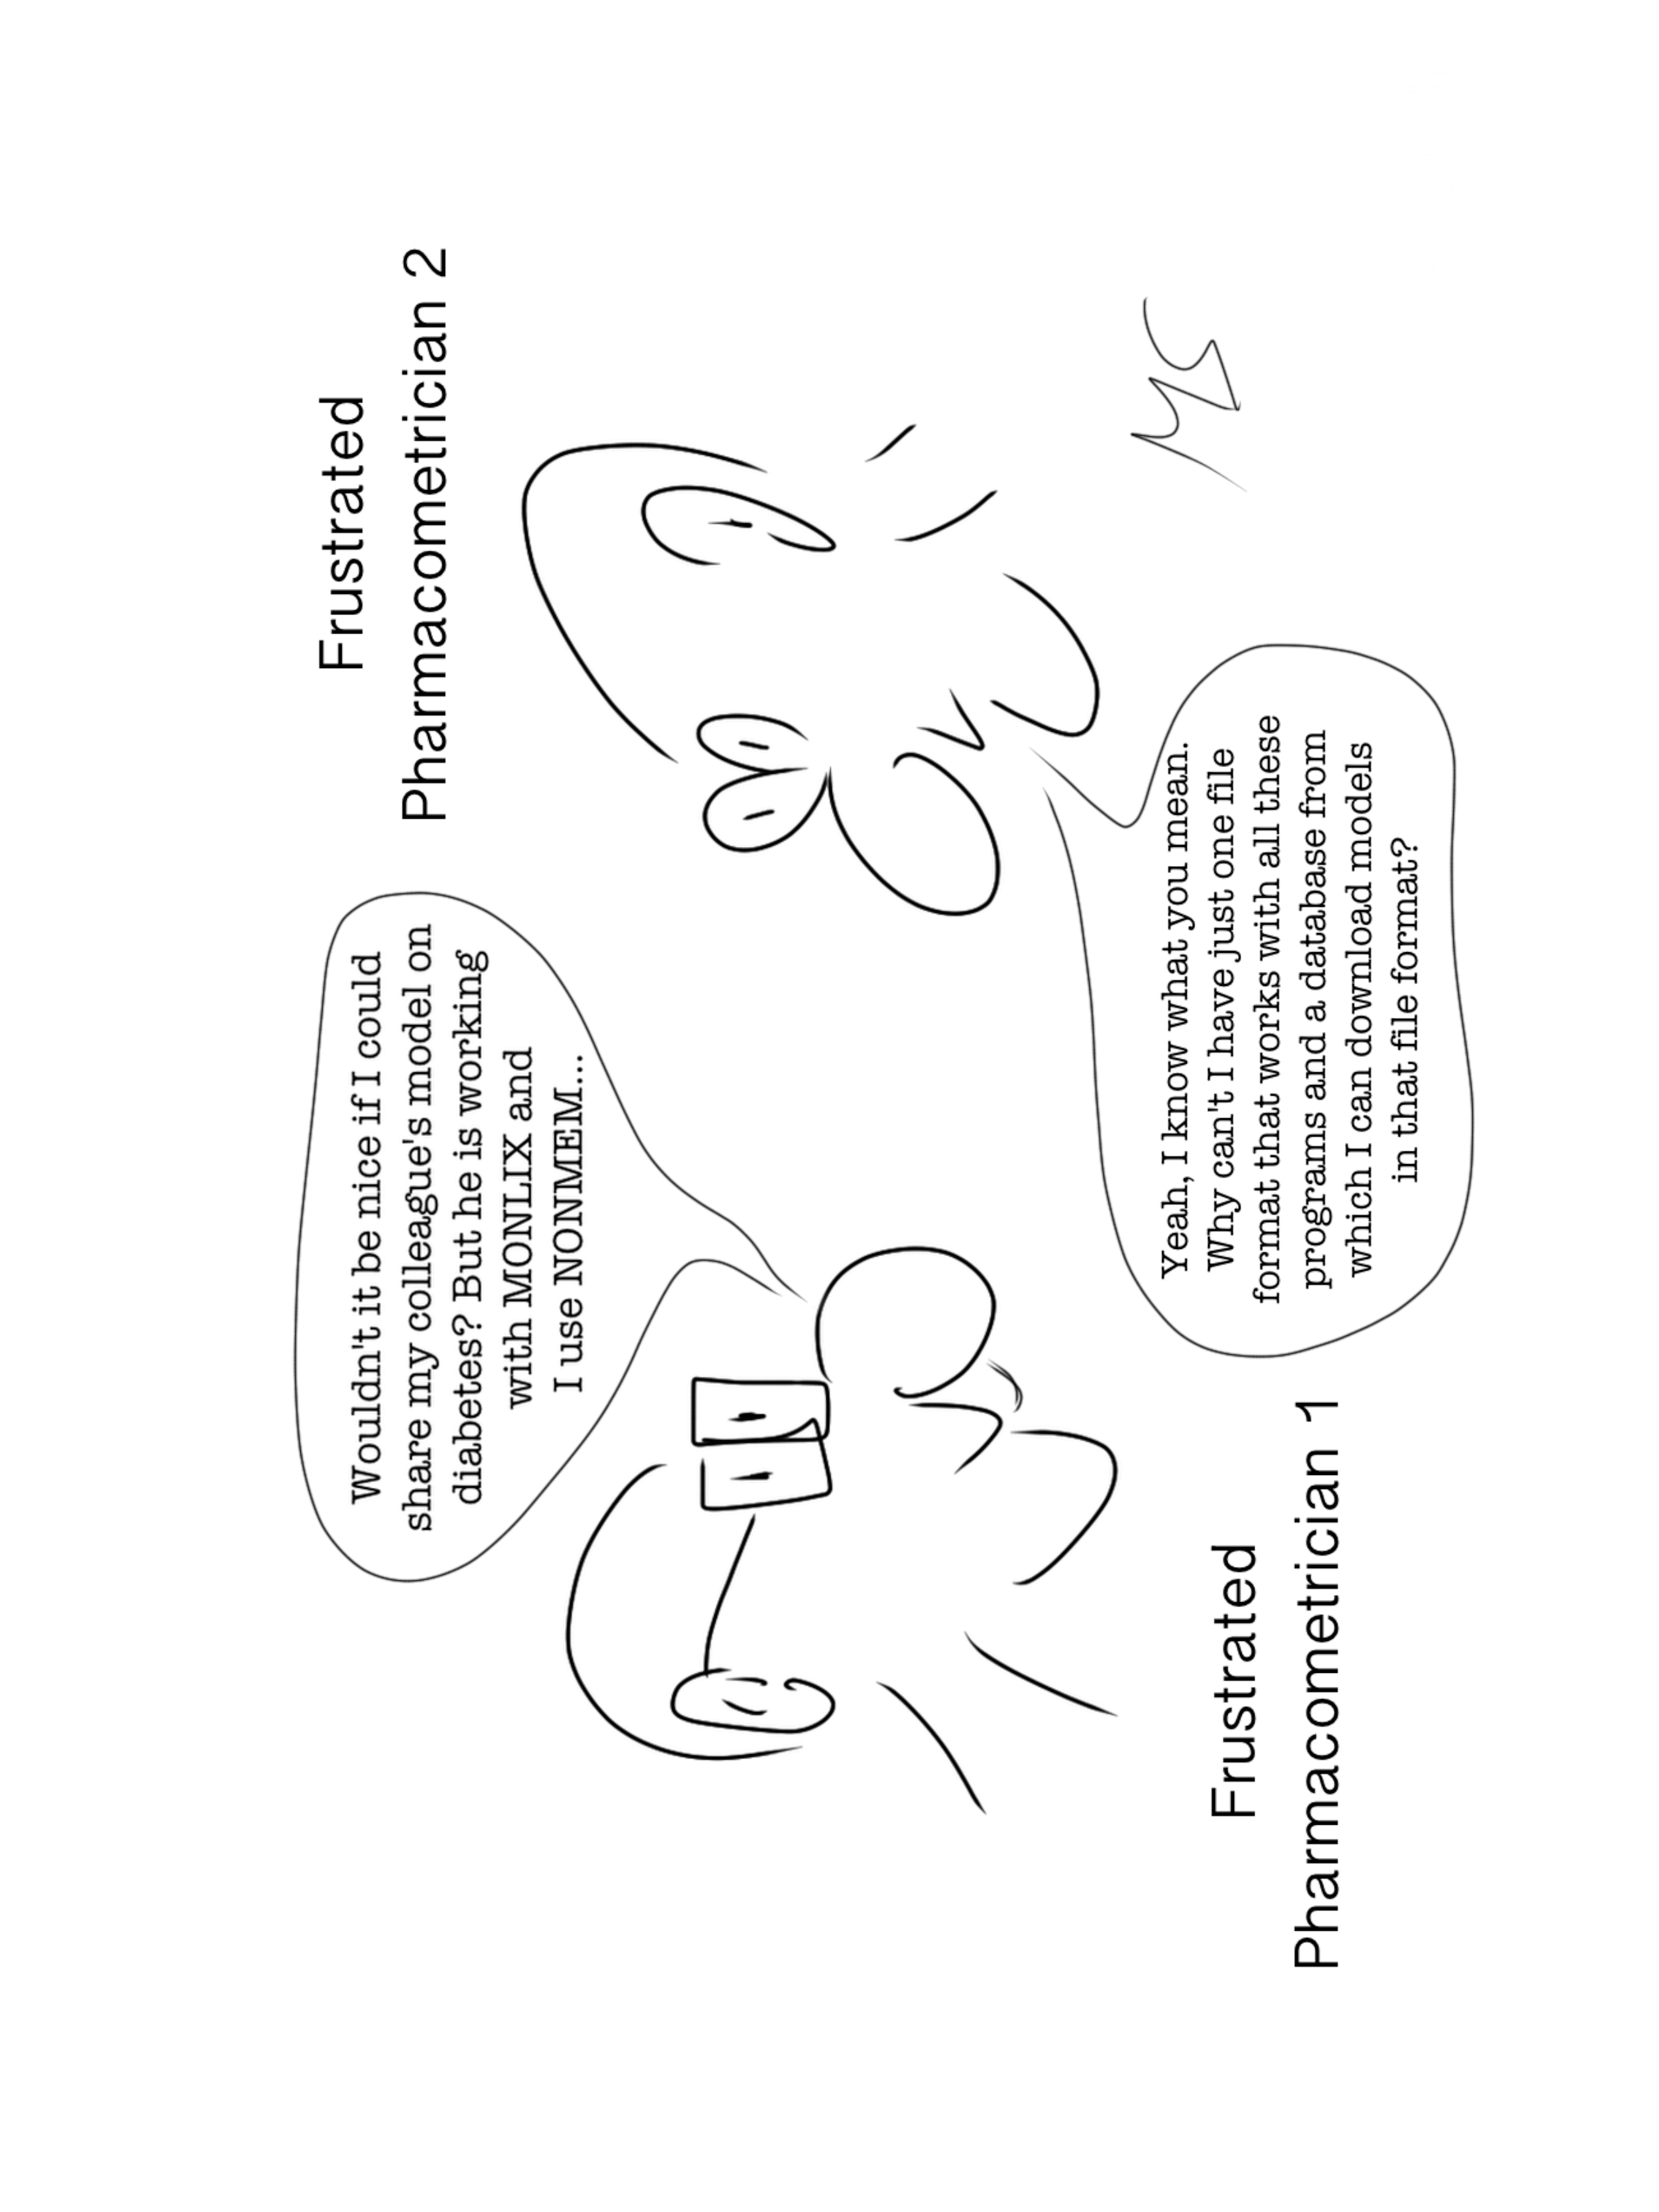
\includegraphics[angle=270,width=\linewidth,trim=90mm 80mm 80mm 50mm]{MMLdudesFinal2}
\end{wrapfigure}
% }
%\end{figure}

%We could add to this cartoon, the caption: ``Someone, somewhere must be trying to solve this problem!''
%And if you read the \ddmore newsletter\footnote{Available from \url{www.ddmore.eu}.}, where this cartoon first featured, you will recall that our reply was, ``Well fortunately they are!'' We think this

The cartoon on the right summarises the principal problem that \pharmml addresses: namely,
the reliable exchange of pharmacometric models between software tools. What we are aiming
for is illustrated in figure~\ref{fig:platformDDMoRe}, where \pharmml is the exchange medium
for pharmacometric models for the main modelling and simulation tools in the field. This is
not an unreasonable goal and has been successfully realised in the field of Systems Biology.

In Systems Biology the problems our Frustrated Pharmacometricans complain of do not exist. Software
tools exchange models using the Systems Biology Markup Language (SBML; \url{www.sbml.org})
\cite{SBML} and many published models can be found in the BioModels Database
(\url{http://www.ebi.ac.uk/biomodels-main/}) \cite{BioModels2010}. Modellers don't worry about the
content of an SBML file; they rely on the fact that when they exchange it between their favourite
modelling tools, it just works. Crucial to its success has been an active community of tool
developers and modellers who have supported and used it during
that time. Equally important has been the provision of sophisticated software libraries (libSBML
and JSBML) that take away much of the pain a software tool developer would otherwise experience
supporting what is now quite a complex standard. It is a virtuous circle. Users demand their
modelling tools support SBML\@. Developers provide reliable SBML support using libSBML, which
enables them to give their users what they want. The more tools that support SBML, the more useful
it becomes. The cost of supporting SBML is not negligible but quality libraries like libSBML make
the cost acceptable.

\begin{figure}[htb]
\centering
  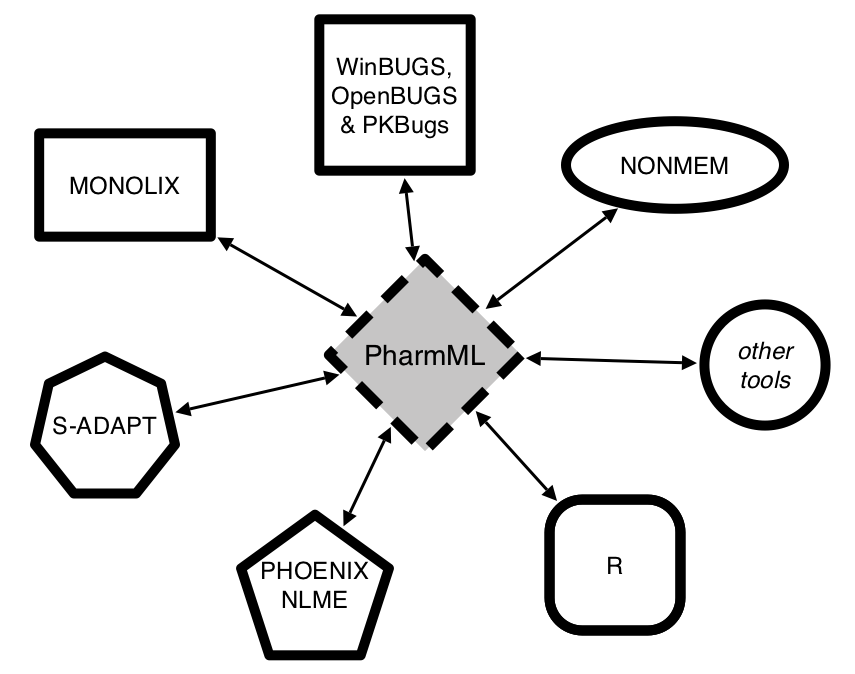
\includegraphics[width=0.5\linewidth]{platformDDMoRe}
 \caption{Interoperability platform to exchange models via \pharmml.}
 \label{fig:platformDDMoRe}
\end{figure}

This lesson has not be ignored by the pharmacometrics community and in fact a number of years
ago the NLME consortium (a consortium of pharmaceutical companies now all part of \ddmore) started
to work on a very similar standard to \pharmml. This resulted in early drafts of an XML based exchange
language, called PharML, but work on it was unfortunately discontinued and the standard has never been
used and validated. There are a number of other exchange standards in related modelling fields, which we
have drawn on in the development of our work to varying degrees, including:

\begin{description}
\item[CellML] Supports the exchange and storage of computer based mathematical models of biological systems \cite{CELLML}.
\item[NeuroML] Supports the exchange and description of models ``to describe the biophysics, anatomy and network architecture of neuronal systems at multiple scales''\footnote{Quoted from \url{http://www.neuroml.org} on 15 Mar 2013.} \cite{NeuroML}.
\item[NineML] Describes neuronal networks in a ``simulator independent language''\footnote{Quoted from \url{http://software.incf.org/software/nineml} on 15 Mar 2013.} that is design to interact with NeuroML \cite{ninemlspec}.
\item[SED-ML] Encodes simulation experiments of SBML and CellML models ``to ensure exchangeability and reproducibility of simulation experiments''\footnote{Quoted from \url{http://sed-ml.org} on 15 Mar 2013.} \cite{sedmll1v1}.
\end{description}

So what is the solution to the problem? \pharmml. An XML based language that will be able to encode
models from NONMEM, MONOLIX, BUGS and related tools. We intend this to be a community standard nucleated
around the members of the \ddmore consortium. In addition we are developing a software library
(libPharmML) to help tool providers incorporate support of \pharmml and to facilitate its
general adoption in the field.

So there is hope for the Frustrated Pharmacometricians. \pharmml will solve the problem.

% \begin{quote}
% {\small
% Nothing is original. Steal from anywhere that resonates with inspiration or fuels your imagination. Select only things to steal from that speak directly to your soul. If you do this, your work (and theft) will be authentic. Authenticity is invaluable; originality is non-existent. And don't bother concealing your thievery -- celebrate it if you feel like it. In any case, always remember what Jean-Luc Godard said: "It's not where you take things from -- it's where you take them to." \\
% \textit{Jim Jarmusch}}
% \end{quote}
% PharmML standardises the formulation and annotation of models used in pharmacometrics. Once a model is encoded in this format, it can flexibly be used for various purposes such as
% \begin{itemize}
% \item
% modelling
% \item
% simulation (e.g. individual subjects or clinical trial simulations)
% \item
% estimation (e.g. population and individual parameters)
% \item
% exploration (e.g. parameter scan/sensitivity, optimal design)
% \end{itemize}
% There are many tools being used in pharmacometrics, such as BUGS (winBUGS \cite{Lunn:2002aa} and openBUGS \cite{Lunn:2009fk}), Monolix \cite{Monolix4.2.1UserGuide:2012}, NONMEM \cite{NONMEM:2009}, PKBugs \cite{PKBUGS:1999}, S-ADAPT \cite{SADAPT:2008}, SimBiology Toolbox \cite{SimBiologyToolbox:2012} or Phoenix NLME \cite{PhoenixNLME:2011} to name only the the most popular.

% However, the current specification has been developed with focus on two tools being used in clinical and pharmaceutical research, NONMEM and Monolix. The choice and the number of tools under consideration had multiple reasons. On one side, the project description dictated the choice and preferences, on the other side the time constraints allowed for proper analysis of only these two tools. Further specifications will consider broader class of tools and approaches, such as Bayesian methods.

% Nevertheless, the differences between these softwares, which manifest themselves mainly in the \textit{imperative} approach of NONMEM versus the \textit{declarative} approach of Monolix, created a chance to a cover broad spectrum of methods and ideas developed over decades. \\
% On the one hand FORTRAN-based NONMEM, despite having a specifically defined language (NM-TRAN \cite{NONMEM:2009}), offers almost
% unlimited flexibility to the user. It can be viewed as a general purpose computational platform and in fact it has been developed
% as such and can be compared to Matlab or Mathematica (REFs). On the other hand Monolix has been specifically developed for use in pharmacometrics. Although being very flexible, it is based on MLXTRAN, a constantly developing declarative language, defining very precisely the types of allowed models and algorithms.
% \\
% It is not the purpose of this document to conduct a detailed comparison between these two approaches but it is important to keep the characteristic differences in mind. One of the main objectives of the DDMoRe project and specifically work-package 4 (WP4) is the building a bridging technology for alternative approaches within one framework. PharmML, the XML based exchange standard which is now available in this first specification is the core element of this interoperability framework.

% \begin{figure}[htb]
% \centering
%   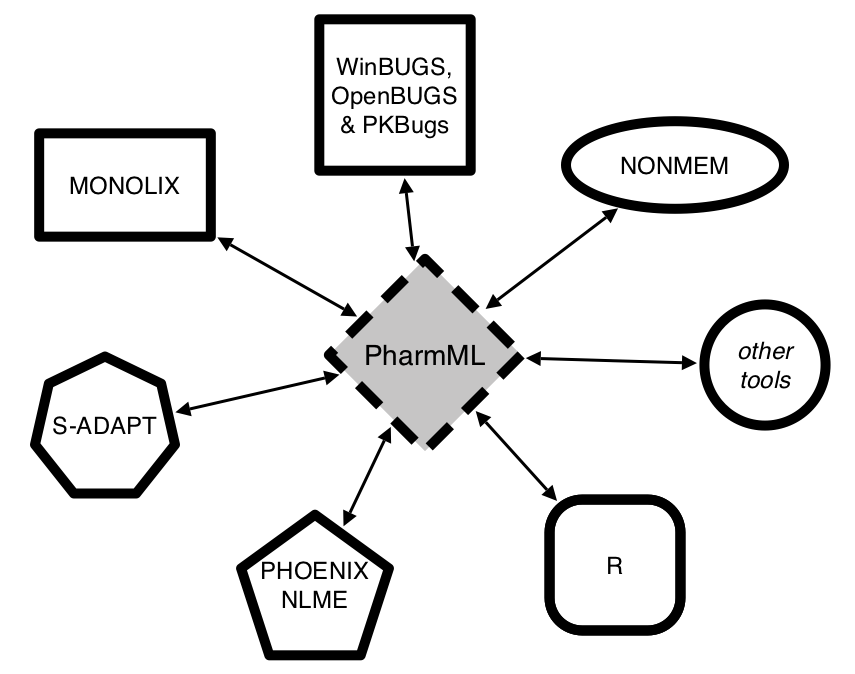
\includegraphics[width=0.9\linewidth]{platformDDMoRe}
%  \caption{Interoperability platform to exchange models via PharmML.}
%  \label{fig:platformDDMoRe}
% \end{figure}

% The idea of XML-based markup languages to represent models and data is not new. In fact, the pharmacometric community around the NLME consortium (REF) started to work on a new format for drug related research and developed an initial concept in form of the PharML standard (REF). The activities have been unfortunately discontinued and the standard has never been used and validated. There is number of other standards in various field of science, such as NeuroML (REF) in neurobiology, PMML (REF) in predictive analytics and data mining, SBML (REF) in Systems Biology or UncertML (REF) designed for encapsulating probabilistic uncertainties. PharmML builds on the experience and results of this effort by reusing those standards were appropriate.


% \section{Intro}

% I'm not sure about the quote at the beginning. I don't think it sets the correct tone. It also doesn't tie into the rest of the introduction. My preference would be to drop it or replace it with something that fits more neatly with what we are doing.

% I think this chapter could be expanded considerably and the current content reorganised.

% The current section doesn't mention the exchange of models, but says it can be used for M\&S, which is misleading. It makes it sound like a rival the MDL, which is it not. It goes on to state that the spec has focused on NONMEM \& Monolix, which is mis-leading as we have focussed on models generally (that why we had discussions with modellers and use general mathematical descriptions in the use case doc) but have wanted to ensure that we can support exchange between NONMEM and Monolix. I think this kind of statement would be better in the scope section. That way as the scope changes we don't need to update chap1 for future revisions. Then the discussion about the nature of imperative or declarative model specification languages, while useful comes far too soon (para 4). I think this should be a later section in this chapter, because it is important to mention it. The last paragraph about other MLs again should be expanded into a full section. It would be useful to go into some detail about SBML and libSBML. Also to include SED-ML too. Also perhaps the COMBINE archive - not sure about that one.

% The following is perhaps a better structure. I think breaking it into the following sections would be a good idea.


% \section{The Problem}

% We should set out the problem. That there is no platform independent way to exchange Pharmacometric models. We should also explain why this is desirable, i.e. what problems it would solve. Perhaps use the analogy of exchanging doscuments using word. No-one cares what the file looks like - it just works most of the time.

\section{The Solution}
\label{intro:objectives}

Having described the problem, we here articulate the \emph{kind} of solution we wanted \pharmml to be.
Developing a language as complex as \pharmml is a difficult undertaking and we wanted to make sure
that we had some firm principles in place to help when designing the language. We've set these aims
and objectives below. \pharmml should:

\begin{description}
%\item[encode models used by pharmacometricians]
\item[describe the mathematics of a model] The language should not include information about the authorship of a model, its update history, or the nature of the disease process or drug that is being modelled. These aspects will be captured by the annotation of the \pharmml document and are out of scope of this specification.
\item[describe the task(s) associated with a model] The task(s), such as simulation or estimation, to be performed with a model should be encoded in the language.
\item[be declarative] The language should describe \emph{what} information is present in a model and \emph{what} the associated task(s) are. It should not describe \emph{how} the information is organised, or \emph{how} the task(s) should be performed.
\item[be platform independent] Language elements specific to a particular modelling tool should not be included. For example it should not describe a structural model using a name specific to PREDPP in NONMEM.
\item[serve as an exchange format for the \ddmore infrastructure] The language should either support features required by the infrastructure or provide extension mechanisms so that additional information can be associated with the \pharmml document.
\item[provide support for ontological annotation] The language should provide a mechanism for it to be annotated with information that is useful to describe the model, but which is beyond the scope of the \pharmml document itself.
\item[enable custom extension] Provide an extensibility mechanism so that software tools can associate additional, possibly tool specific information, with a \pharmml document.
\item[reuse existing standards where appropriate] Where an established information standard exists that can be used to represent information within the \pharmml document, we should adopt it.
\end{description}

% Here we say what our aims and objectives were in designing PharmML. This is different to scope because it describes the high-level aims and objectives for PharmML that will not change in future releases of the standard. For example:

% - encode models used by pharmacometricians
% - platform independence
% - declarative
% - describe the mathematics of the model. For example, not the underlying medical condition or drug it is modelling (that is annotation/metadata).
% - Describe model and task
% - Serve as an exchange format for WP2 infrastructure.
% - Provide support for ontological annotation
% - Enable custom extension.
% - Reuse existing standards where appropriate.

\section{The \ddmore Consortium}

%Taken from the DDMoRe website need more work.

The Drug Disease Model Resources (DDMoRe) consortium aims to promote collaborative drug and disease
modelling and simulation research. Its aim is to develop tools and standards that will help the
consortium members and later the wider scientific community achieve this goal. Providing \pharmml
is a key goal of the consortium as it underpins a number of related deliverables of the consortium.
In particular:

\begin{itemize}
\item The \ddmore infrastructure in which \pharmml is used to exchange models between the different modelling tools.
\item The \ddmore model repository in which \pharmml will be used to upload and export models to and from the repository. It will also serve as the storage medium for the repository.
\item The \ddmore library of reference models and data-sets, which will provide models in several therapeutic areas. These models will be encoded using \pharmml.
\end{itemize}

The contribution of the \ddmore consortium members in guiding and reviewing the standard has been enormous.
As the standard evolves their role in using and then promoting the standard to the wider community will be invaluable.

\section{How \pharmml was developed}

We, the authors, have organised and designed \pharmml, but its development has very much been a
collaborative process. When embarking on this project we had a number of development guidelines that we adhered to.
We aimed to:

\begin{itemize}
\item start with a limited scope and expand the functionality we encode over time.
\item drive development using use cases which reflect the current scope.
\item test the implemented use cases by generating executable models.
\item have frequent review meetings with experts to make sure we are on the right track.
\item use existing technology standards if it is possible and reasonable to do so.
\item use existing information standards if applicable to avoid re-inventing the wheel.
\item make sure the standard is in a form and uses names and terms that make sense to the expert community.
\end{itemize}

The use-case based development cycle is illustrated in figure \ref{fig:devcycle} and you can see
how the generation of `executable' prototype models was important in ensuring assumptions were
correct before expanding the scope of the design. For this to be possible the use cases were
documented with a mathematical description and the expected outputs and results of the model were
also described in detail \cite{Swat:2013aa}. In some cases reference \matlab\xspace implementations were also included to
assist prototype code generation. Although this development cycle was our objective, in the later
stages there was insufficient time to upgrade the code generation framework to produce executable models
from a \pharmml document. Consequently some parts of the specification, in particular the parts related
to estimation tasks, have not been tested as thoroughly as we would like.

\begin{figure}[htb]
\centering%
 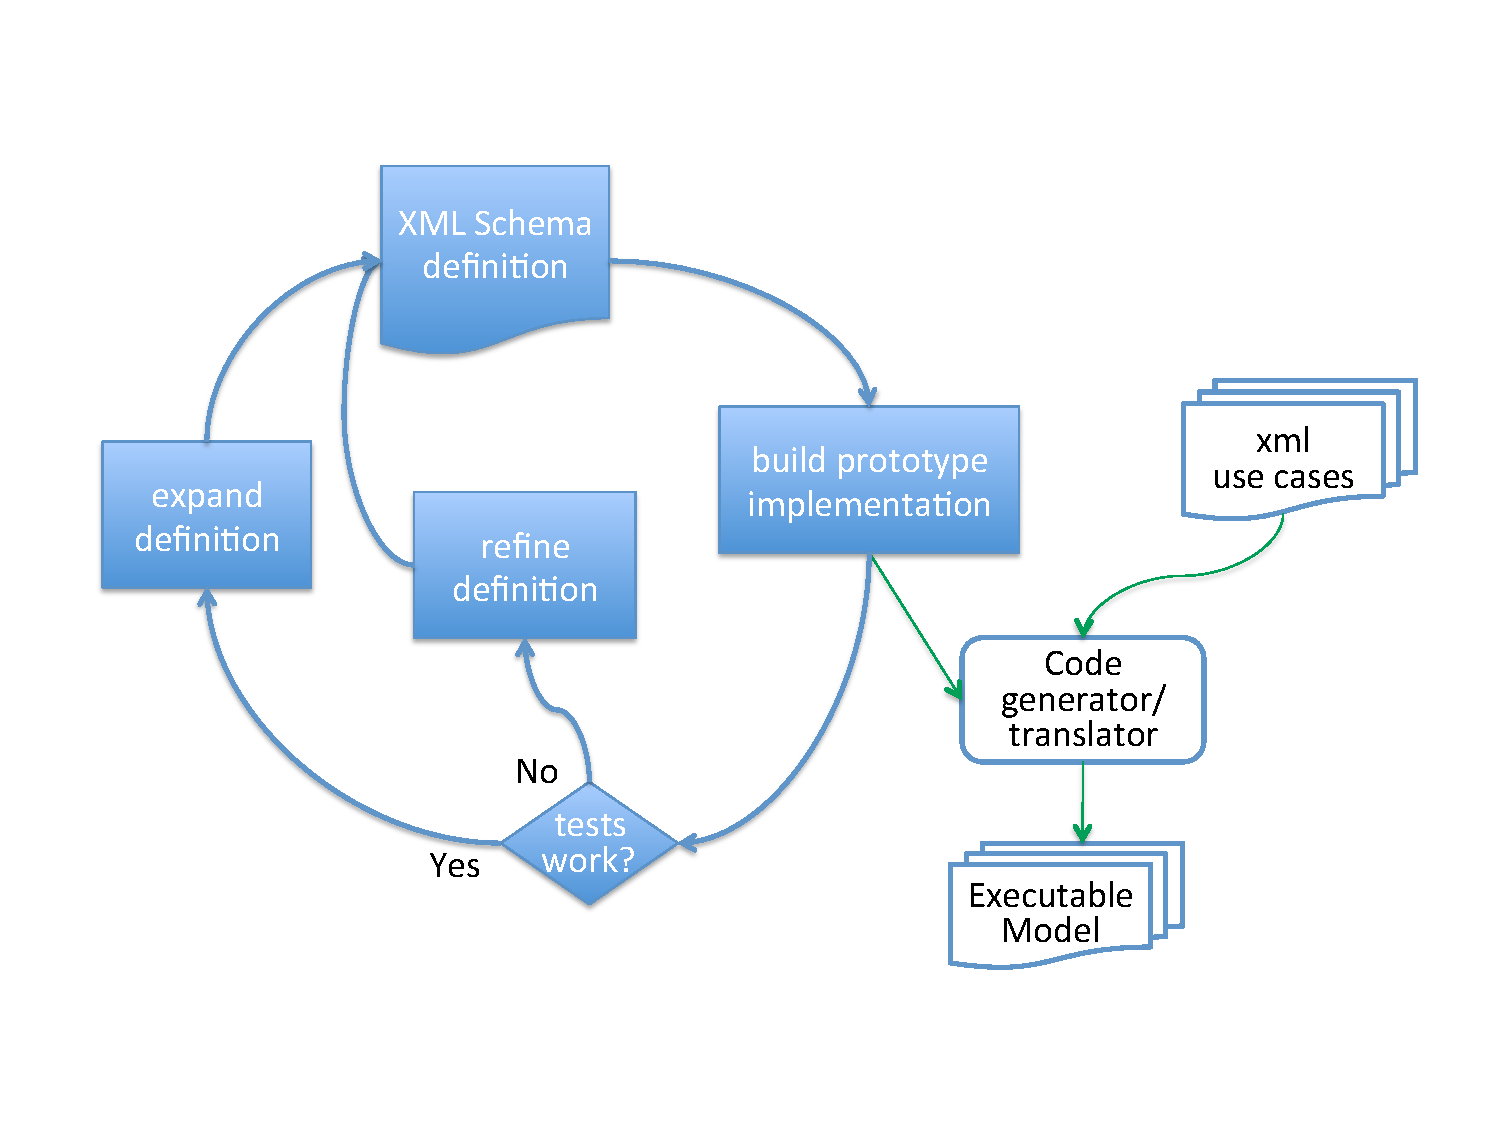
\includegraphics[width=0.7\linewidth,trim=10mm 20mm 20mm 10mm]{devcycle}
\caption{An overview of the development cycle adopted by the \pharmml team.}
\label{fig:devcycle}
\end{figure}


Peer review is important in the development of \pharmml and to date we have hosted three face-to-face
review meetings since the development of \pharmml commenced in August 2011. These meetings were:

\begin{itemize}
\item The \ddmore consortium meeting in Leiden, 24--26 Apr 2012.
\item The \ddmore consortium meeting in Noordwijkerhout, 11--13 Sep 2012.
\item The \ddmore technical workshop hosted by Novo Nordisk in Copenhagen, 28--30 Jan 2013.
\end{itemize}

\section{Imperative or Declarative?}

In developing \pharmml we have designed it to be a declarative language (see section \ref{intro:objectives}).
While we feel this is the best approach to take for an information exchange langage, it does present us
with number of challenges when dealing with NONMEM, the leading tool in the field. Despite
having a specifically defined language (NM-TRAN \cite{NONMEM:2009}), NONMEM offers a lot of flexibility
to the user, and experienced users can make NONMEM do things that it was never designed to do, to a large
extent because the imperative approach used in NONMEM facilitates this.

The challenge is to convert from the imperative to the declarative language, because there are usually many
ways to do the same thing in the imperative language. Therefore, generating a \pharmml document from a NONMEM
control stream may be challenging.

 % It is not the purpose of this document to conduct a detailed comparison between these two approaches but it is important to keep the characteristic differences in mind. One of the main objectives of the DDMoRe project and specifically work-package 4 (WP4) is the building a bridging technology for alternative approaches within one framework. PharmML, the XML based exchange standard which is now available in this first specification is the core element of this interoperability framework.

 % Nevertheless, the differences between these softwares, which manifest themselves mainly in the \emph{imperative} approach of NONMEM versus the \emph{declarative} approach of Monolix, created a chance to a cover broad spectrum of methods and ideas developed over decades. On the one hand FORTRAN-based NONMEM, despite having a specifically defined language (NM-TRAN \cite{NONMEM:2009}), offers almost
 % unlimited flexibility to the user. It can be viewed as a general purpose computational platform and in fact it has been developed
 % as such and can be compared to Matlab or Mathematica (REFs). On the other hand Monolix has been specifically developed for use in pharmacometrics. Although being very flexible, it is based on MLXTRAN, a constantly developing declarative language, defining very precisely the types of allowed models and algorithms.

 % It is not the purpose of this document to conduct a detailed comparison between these two approaches but it is important to keep the characteristic differences in mind. One of the main objectives of the DDMoRe project and specifically work-package 4 (WP4) is the building a bridging technology for alternative approaches within one framework. PharmML, the XML based exchange standard which is now available in this first specification is the core element of this interoperability framework.

%Let's put the NONMEM Monolix discussion here and then say that we have adopted a declaritive approach and say why it is better. Need to be careful %here to make sure we don't imply that in consequence Monolix is better than NONMEM.

\section{The Evolution of PharmML}

This document represents the start of an evolution for \pharmml. Any piece of software is upgraded as
users request new features and developers find better ways to do the same thing. A successful standard
is no different and with success in mind we expect \pharmml to evolve and change as it is subject to the
same influences. To manage this process we plan to adopt the following strategy to record versions of
the \pharmml specification.

\subsection{Version number}
\label{intro:versioning}

To record changes in the specification we will use the following three level numbering system, of the form
$x.y.z$. The levels correspond to the following types of revision:

\begin{description}
\item[$x$ major] Significant new features or radical change of design. Not backwards compatible.
\item[$y$ minor] New features or evolutionary design changes. Always backwards compatible.
\item[$z$ patch] Error corrections. Always backwards compatible.
\end{description}

By backwards compatible we mean that a \pharmml parser that supports version 1.9.0 must be able to read
a file that is compliant with version 1.4.0 of the \pharmml specification.

\subsection{Release Process}

Before each release we will submit a release candidate of the specification to the community for comments
and criticism. This is typically called a Request for Comments (RFC) and is standard practise. Based on
review comments the specification will either be revised, possibly significantly, and submitted for review
again or (if revisions are minor) revised and released.

The RFC period for this specification will end on 26 April 2013.

\section{Feedback}

Whether it is during the RFC process or after a release your feedback is important to us. Typically,
this feedback will be in the form of a specific issue: either to report defects you have identified in
the specification or to request new features. Either way we would urge you to submit specific issues to
our tracker at: \url{sf.net/ddmore/tracker}. In some cases you may wish to ask for clarification or raise
an issue that is broader than a specific issue or requires some discussion within the community. Here you
should contact the \pharmml forum at \url{sf.net/ddmore/forum}.


% What is PharmML? Why is it useful.

% High level aims and objectives in designing it.

% How we went about designing it.

% Past work. Other influences?


\chapter{This Document}
\label{chap:this-document}

% Overview of this spec. How to read it etc.

\section{Overview}

In this specification we describe the \pharmml standard. We define what the language is, how it is encoded,
how it should be understood, and how software can validate it. Initially, we define in chapter \ref{chap:scope}
what is in and out of scope of the current version of \pharmml. Underlying \pharmml is a mathematical model
that describes a pharmacometric model. Understanding this is important if you are to completely understand
the language. In chapter \ref{chap:mathsdefn} we go through this model in detail, providing a detailed
mathematical description of the model and its associated assumptions. Also important for the understanding of
\pharmml is the discussion of trial designs in chapter \ref{sec:CTS}, where the basic assumptions behind
the way trial designs are handled in \pharmml are discussed. Next we move on to
the description of the implementation of \pharmml. In chapter \ref{chap:lang-overview} we describe the
organisation of a \pharmml document and then go on to explain key features of the language, such as variable
scoping, that are important to understand before investigating the language further. Chapter \ref{chap:worked-egs}
explains the details of \pharmml using examples. These examples are designed to highlight specific features of
the language and by taking you through a series of worked examples we hope to help you to fully understand \pharmml.
The final chapter in Part \ref{part:primer} (Chapter \ref{chap:unresolved}) lists a number of unresolved issues.

At the end of this document we have the technical reference (Part \ref{part:techref} on page \pageref{part:techref}).
This provides the fine detail of the technical implementation of \pharmml, including the XML Schema design and
the rules to which a correct \pharmml document must conform. This is reference material and not intended to be
read like a novel  from start to finish.

To conclude, helping you to understand \pharmml is the main goal of this specification. We want you to use this
document to review and critique \pharmml. We want you to suggest improvements to the language. Most of all
we want you to use it.

\section{How to read this Specification}

\pharmml is a language of benefit to pharmacometric modellers, but ironically is not designed to be read by
them when in every day use. We expect software support for \pharmml to be developed by software engineers,
who do not have a deep understanding of pharmacometrics and modelling. Therefore, the challenge for us in
drafting this specification is to satisfy both readerships: modellers and software engineers. To help, we
have come up with the following advice on how each readership could read this specification.

If you are a pharmacometric modeller or mathematician then you will want to start with the mathematical
definition of \pharmml in chapter \ref{chap:mathsdefn} (page \pageref{chap:mathsdefn}). From there you
may want to skim the language overview (chapter \ref{chap:lang-overview}) before working through the
examples in chapter \ref{chap:worked-egs} (page \pageref{chap:worked-egs}). You may want to revisit
chapter \ref{chap:lang-overview} (page \pageref{chap:lang-overview}) after reading the examples.

If you are a software engineer then we recommend that you start with the language overview in chapter
\ref{chap:lang-overview} (page \pageref{chap:lang-overview}). After this, work through the examples
in chapter \ref{chap:worked-egs} (page \pageref{chap:worked-egs}) and try to understand the language
features in this way. Those of you with a strong mathematics background will find it helpful to read
through the mathematical definition as well (chapter \ref{chap:mathsdefn}). Finally, when it comes to
implementing \pharmml support, you will find the technical reference (Part \ref{part:techref} on
page \pageref{part:techref}) very important, but only after you have an understanding of \pharmml
from Part \ref{part:primer}.

%\section{Conventions used in this document}

%I'm sure there are some. We should put something here!!!!


%\part{Theoretical Representation}

% This section deals with the scope and the mathematical definition
% that we represent in PharmML

% from the input folder
%\renewcommand*{\descriptionlabel}[1]{\hspace\labelsep\normalfont\sffamily #1}
\newenvironment{features}{%
\firmlists\begin{description}}%
{\end{description}}
\newcommand\feat[1]{\item[-- \normalfont\itshape #1]}


\chapter{Features supported by \pharmml}
\label{chap:scope}


\section{Introduction}

The scope of pharmacometric models is very wide, as such models can be empirical as well as
mechanistic; describe continuous as well as discrete data types; and be deterministic, stochastic
or a mixture of both. It is a challenging endeavour to accommodate this variety of possibilities
under one computational standard, therefore it is indispensable to split the task into multiple
steps of subsequent specifications and to define precisely the scope of every release.

In this chapter we define the scope of the functionality in
\pharmml. In particular what information a \pharmml document can
represent and what it cannot. As is common practise in software
engineering we have described the functionality as a set of
``features''. These features are said to be \emph{current} if they are
provided by this release of \pharmml, \emph{planned} if they are not
in the current version, but planned for a future release.
% and \emph{not  include} if we wish to highlight the fact that we believe \pharmml
%will not include this feature. 
It is important to remember that this
specification is just the beginning of \pharmml and over time we
expect many of the features currently out of scope to be provided by
future releases of the language.

The language is organised into three sections, which we believe naturally
describe the logical organisation of a pharmacometric model and its
associated tasks. Consequently we have grouped the features to match this
organisation. The sections are:
\begin{description}
\item[Model Definition] A description of the model, incl.\ the structural model, the model
  parameters, relevant covariates, the variability components, and the observations.
\item[Trial Design] A description of the design of a clinical trial associated with the model
  (for example a trial from which data is available to estimate the parameters of the model or
  a trial to be simulated with the model).
\item[Modelling Steps] A description of steps or tasks performed with
  the model. Typically this describes how the model has been used, for
  example to estimate its parameters or to perform a simulation.
\end{description}


\section{Current Features}

\subsection{General}

\begin{features}
\feat{Metadata annotation} Provides support to enable metadata
descriptions of the \pharmml document.
\feat{Extension mechanism} Provides support to enable the extension of
the \pharmml document.
\end{features}

\subsection{Model Definition}

\subsubsection{Structural Model}

\pharmml can encode:
\begin{features}
\feat{A structural model defined by a set of algebraic equations.} Typically the explicit solution to a simple PK model, or a dose-response model.
\feat{A structural model defined by a system of ODEs with initial conditions.} Such systems of ODEs can include algebraic equations as well.
\feat{A structural model defined in \sbml format.}
\feat{A structural model from an external resource or library.}
\feat{Standard PK models} Including those encoded by Monolix \cite{Bertrand:2008} or PREDPP in NONMEM \cite{PREDPP:2011}.
\feat{Standard PD models.} Including those defined by Monolix \cite{Bertrand:2008}.
\end{features}

\subsubsection{Covariate Model}

\pharmml can encode:
\begin{features}
\feat{Continuous covariates.} These can be sampled from a probability distribution and used with an applied transformation.
\feat{Categorical covariates.} These can also be sampled from a probability distribution.
\end{features}

\subsubsection{Parameter Model}

%\footnote{As described in detail in section \ref{maths:parameter-model}, the current specification allows encoding of models that are linear in the transformed parameter, which covers the majority of cases in practical applications. This approach is
%flexible in that one can encode any type of parameter with a distribution that is normal up to a transformation, i.e.
%normal (identity transformation), log-normal (natural logarithm) or logit-normal (logit tranformation).}

\pharmml can encode:
\begin{features}
\feat{The population mean/typical value for a parameter.}
\feat{Linear covariate model.}
\feat{Random effects at arbitrary levels of variability.}
\feat{Correlation of the random effects, described by a correlation or covariance matrix.}
\feat{Non-linear parameter models, such as those described in \cite{Keizer:2011aa}.}
\end{features}

\subsubsection{Variability Model}

\pharmml supports the following levels of variability:
\begin{features}
\feat{Between-Subject Variability (BSV).} Aka inter-individual variability (IIV).
\feat{Inter-Occasion Variability (IOV).} Such as within-subject variability.
\feat{Higher levels of variability above BSV.} Such as variability between countries or centres.
\feat{Lower levels of variability below IOV.} Such as variability between sub-occasions within occasions.
\end{features}

\subsubsection{Observations Model}

\pharmml currently only supports the following observation model:
\begin{features}
\feat{Continuous observation model.} A residual error model applied to one or more variables in the structural model.
\feat{Autocorrelation of the residual errors in a continuous observation model.}
\end{features}

\subsection{Trial Design}

\pharmml can encode the following features of a trial design \emph{explicitly}\footnote{As
opposed to the implicit trial design definition present within a data file.}:
\begin{features}
\feat{Bolus dosing.}
\feat{Infusion dosing.}
\feat{Multiple dosing regimens including mixed bolus and infusion.}
\feat{Repeated dosing.}
\feat{Dosing at arbitrary time points.}
\feat{Steady state dosing.}
\feat{Dosing to more than one compartment.}
\feat{Cross-over designs.}
\feat{Parallel designs.}
\feat{Washout periods.}
\feat{Run-in periods.}
\feat{Occasions -- defined by time interval within a treatment epoch.}
\feat{Trials with different centres or other levels of organisation above study groups (aka arms)}
\end{features}

\subsection{Modelling Steps}

\pharmml can encode the following features related to the task(s) associated with a model:
\begin{features}
\feat{Estimation utilising the maximum likelihood principle.}
\feat{Simulation of the model}
\end{features}


\section{Planned Features}

\subsection{General}

\begin{features}
\feat{Units} Support for unit definitions and unit consistency
checking.
\end{features}

\subsection{Model Definition}

\subsubsection{Covariate Model}

\pharmml does not support the following covariate related features:
\begin{features}
\feat{Conditional distributions of continuous covariates.}
\feat{Clusters of categorical covariates.}
\feat{Selection/exclusion criteria for covariates.}
\end{features}

\subsubsection{Structural Model}

\pharmml does not support the following model types:
\begin{features}
\feat{(Hidden) Markov models.}
\feat{Delay Differential Equations (DDEs).}
\feat{Partial Differential Equations (PDEs).}
\feat{Stochastic Differential Equations (SDEs).}
\end{features}

\subsubsection{Observations Model}

\pharmml does not support the following types of observation models:
\begin{features}
\feat{Count data models.} Poisson, negative binomial, zero-inflated Poisson models etc.
\feat{Nominal and ordered categorical models.} Logistic regression, proportional odds models etc.
\feat{Time-to-event models.} Parametric (e.g.\ exponential, Gompertz, Weibull) or semi-parametric Cox models.
\end{features}

\subsection{Trial Design}

\pharmml cannot encode the following features in a trial design:
\begin{features}
\feat{Reset of all or single compartments.}
\end{features}

\subsection{Modelling Steps}

\pharmml cannot encode the following features related to the task(s) associated with a model:
\begin{features}
\feat{Bayesian inference methods.}
%Methods such as Maximum a posteriori (MAP) or Bayesian inference sing Gibbs sampling methods used in tools of the BUGS-family (winBUGS \cite{Lunn:2002aa}, openBUGS \cite{Lunn:2009fk}) or JAGS \cite{JAGS:2003aa}.
\feat{Writing estimation results to a file or other external resource.}
\feat{Writing simulation results to a file or other external resource.}
\feat{Exchange of results from one modelling step to another.} Currently it is not possible to pass on the results of an estimation task to a subsequent estimation step.
\feat{Model exploration} Tasks such as sensitivity analysis are not
supported.
\feat{Optimal design}
\end{features}

%\section{Features not Included}
%
%\subsection{Model Definition}
%
%\subsubsection{Structural Model}
%
%\pharmml cannot encode:
%\begin{features}
%\feat{Higher order differential equations.}
%\feat{Delay Differential Equations (DDEs).}
%\feat{Partial Differential Equations (PDEs).}
%\feat{Stochastic Differential Equations (SDEs).}
%\feat{(Hidden) Markov models.}
%\end{features}

%\subsubsection{Covariate Model}
%
%\pharmml cannot encode:
%\begin{features}
%\feat{Conditional distributions of continuous covariates.}
%\feat{Clusters of categorical covariates.}
%\feat{Selection/exclusion criteria for covariates.}
%\end{features}



% \begin{itemize}
% \item
% ODE based, standard 1-, 2- or 3-compartmental or physiology based PK (PBPK) models
% \begin{itemize}
% \item
% defined explicitly as a system of ODE's
% \item
% defined as an SBML model
% \end{itemize}
% \item
% algebraic expressions, if analytic solutions are available, e.g. one-compartmental oral model, see section \ref{sec:structuralModel}
% \item
% using library models, e.g. Monolix \cite{Bertrand:2008} or PREDPP \cite{PREDPP:2011}
% \end{itemize}

% \paragraph{Continuous PD models}
% \begin{itemize}
% \item
% ODE based -- e.g. turnover models
% \item
% algebraic -- e.g. Emax-models
% \item
% using library models, e.g. Monolix \cite{Bertrand:2008}
% \end{itemize}


% \section{MS Intro}

% Any part of human and animal anatomy and physiology can be subject to pathological changes and eventually diseases. The scope of pharmacometric models, dealing with virtually any type of such cases, is therefore almost without precedence in science. The models can be
% \begin{itemize}
% \item
% phenomenological or mechanistic
% \item
% they have to cope both with continuous and discrete data types
% \item
% they are deterministic, stochastic or mixture of both
% \item
% they cover all levels of complexity from the molecular to organ and whole body level
% \end{itemize}
% It is a challenging endeavour to accommodate this variety of possibilities under one computational standard but thanks excellent use cases and other documents created and provided by our DDMoRe partners it seams possible. However it is indispensable to split the task into multiple steps of subsequent specifications and to define precisely the scope of every release. This is exactly the goal of this chapter.


% \section{Components of a pharmacometric model}
% In the context of PharmML a typical pharmacometric model can be decomposed into the following components
% \begin{itemize}
% \item
% Data model
% \item
% Trial design model
% \item
% Structural model
% \item
% Parameter model
% \begin{itemize}
% \item
% Covariate model
% \item
% Variability model
% \item
% Correlation of random effects
% \end{itemize}
% \item
% Residual error model
% \item
% Observation model
% \item
% Task model
% \end{itemize}
% In the following sections we describe each of these components briefly and list features which are implemented in the current specification and those which will be included in future releases (the latter listed in the subsections \textit{\textbf{Out of scope}}).

% \section{Features in and outside of current scope}

% \subsection{Data model}

% Coming soon...


% \subparagraph{Out of scope}
% \begin{itemize}
% \item
% trials with different centres or other levels of organisation above study groups (aka arms)
% \item
% levels of variability below one level of inter-occasion variability
% \item
% dose escalation methods, e.g. accelerated titration designs or pharmacologically guided dose escalation
% \item
% complex dosing models, e.g. Higuchi or Weibull release models
% \item
% reset of all or single compartments
% \item
% output compartment definition
% \end{itemize}

% \subsection{Structural model}
% In the current specification only continuous models are considered and any model which can be formulated using
% as system of ordinary differential equations (ODE) or algebraic equations can be implemented. More precisely, the following options are available
% \paragraph{PK models}

% \begin{itemize}
% \item
% ODE based, standard 1-, 2- or 3-compartmental or physiology based PK (PBPK) models
% \begin{itemize}
% \item
% defined explicitly as a system of ODE's
% \item
% defined as an SBML model
% \end{itemize}
% \item
% algebraic expressions, if analytic solutions are available, e.g. one-compartmental oral model, see section \ref{sec:structuralModel}
% \item
% using library models, e.g. Monolix \cite{Bertrand:2008} or PREDPP \cite{PREDPP:2011}
% \end{itemize}

% \paragraph{Continuous PD models}
% \begin{itemize}
% \item
% ODE based -- e.g. turnover models
% \item
% algebraic -- e.g. Emax-models
% \item
% using library models, e.g. Monolix \cite{Bertrand:2008}
% \end{itemize}

% \subparagraph{Out of scope}
% The following model types or approaches are planned for a subsequent release
% \begin{itemize}
% \item
% Discrete data models
% \begin{itemize}
% \item
% nominal and ordered categorical models e.g. logistic regression, proportional odds models etc.
% \item
% count data models, e.g. Poisson, negative binomial, zero-inflated Poisson models etc.
% \item
% time-to-event models, e.g. parametric (e.g. exponential, Gompertz, Weibull) or semi-parametric Cox model
% \end{itemize}
% \item
% (Hidden) Markov models
% \item
% stochastic differential equations (SDE)
% \item
% delay differential equations (SDE)
% \item
% partial differential equations (PDE)
% \end{itemize}


% \subsection{Parameter model}
% As described in detail in section \ref{sec:parameterModel}, the current specification allows for encoding of
% models which are linear in the transformed parameter which covers a majority of cases in practical applications.
% This approach is flexible in that one can encode any type of parameter which distribution is normal up to a transformation,
% i.e. normal (identity transformation), log-normal (natural logarithm) or logit-normal (logit tranformation).\\
% The parameter model consists of the following elements
% \begin{itemize}
% \item
% population/typical value for the parameter
% \item
% continuous and categorical covariate model (covariates can be sampled from probability distributions)
% %---- estimating categorical distribution from external data file \\
% %---- sampling from known categorical distribution \\
% \item
% random effects of arbitrary level, see section \ref{sec:variabilityModel} for details
% \item
% correlation of random effects, described by a correlation or covariance matrix
% \end{itemize}

% \subparagraph{Out of scope}
% The following features are planned for a subsequent release:
% \begin{itemize}
% \item
% non-linear parameter models, such as those described in \cite{Keizer:2011aa}
% \item
% autocorrelation of residual errors
% \item
% clusters of categorical covariates
% \item
% conditional distributions of continuous covariates
% \item
% selection/exclusion criteria for covariates
% \end{itemize}


% \subsection{Residual error model}
% PharmML is flexible with respect to defining residual error models. Currently this can be done
% only explicitly as there is no external library, see section \ref{sec:residualErrorModel}.
% For a future release the creation of an external library is planned.

% \subsection{Observation model}
% The following information can be stored in PharmML
% \begin{itemize}
% \item
% model variable to be observed, both for continuous PK or PD models
% \item
% time points for every model varaiable at which predictions are to be estimated
% \end{itemize}

% \subsection{Task model}
% This model describes a combination of the operations one can perform on the model, such as:
% \begin{itemize}
% \item
% simulation of a trial design, defined explicitly in PharmML or encoded in a data file
% \item
% estimation of population or individual parameters
% \begin{itemize}
% \item
% using the trial design designed in PharmML and objective data encoded in a data file
% \item
% using the trial design and objective data encoded in a data file
% \end{itemize}
% \item
% model exploration, e.g. sensitivity analysis
% \end{itemize}

% \subparagraph{Out of scope}
% \begin{itemize}
% \item
% export of simulation results to an external file
% \item
% export of estimation results to an external file
% \item
% transfer of results from one modelling step to another, for example transferring estimation results to a simulation step
% \end{itemize}


% \paragraph{Inference methods supported in PharmML}
% In general the current specification is restricted to estimation methods utilising the maximum likelihood principle. Not in the scope are Bayesian inference methods such as Maximum a posteriori (MAP) or Bayesian inference sing Gibbs sampling methods used in tools of the BUGS-family (winBUGS \cite{Lunn:2002aa}, openBUGS \cite{Lunn:2009fk}) or JAGS \cite{JAGS:2003aa}.



% %\paragraph{Covariate model}
% %Covariate model is barely covered so far. See also \cite{Keizer:2011aa}. Missing are following features:\\
% %For categorical covariates:\\
% %-- categorical distribution of categorical covariates \\
% %---- estimating categorical distribution from external data file \\
% %---- sampling from known categorical distribution \\
% %---- clusters of categorical covariates \\
% %For continuous covariates:\\
% %-- power-normal distribution for continuous covariates \\
% %---- estimating parameters $\lambda$,$\mu$,$\sigma$ from external data file \\
% %---- sampling from known power-normal distribution \\
% %---- conditional distribution of continuous covariates \\
% %------ none \\
% %------ defined \\
% %------ to be estimated \\
% %---- selecting criteria for continuous covariates \\
% %---- dependent distribution of continuous covariates \\
% %---- correlated continuous covariates \\
% %For both types: \\
% %-- selection/exclusion criteria missing \\
% %
% %\subsection{Observation model}
% %- Name\\
% %- Units\\
% %- Observation types - continuous/discrete\\
% %- Symbol of predicted output\\
% %
% %\subsection{Task model}
% %-- Combination of tasks, e.g.\\
% %1. estimate distribution of covariate from experimental data\\
% %2. Simulation task using the estimated PDF
% %
% %
% %\subsection{Not covered so far}
% %- correlation of residual errors \\
% %---- number models of relevant models identified and described in Use Case document\\
% %


% \newenvironment{features}{\begin{description}}{\end{description}}
\newcommand\feat{\item[]}

\clearpage

\section{Features in Scope}

\subsection{Model Definition}

\pharmml can encode in a model:
\begin{features}
\feat Arbitrary level of variability, both levels lower and higher than between subject variability.
\feat Continuous covariates.
\feat Categorical covariates.
\feat Population parameters.
\feat Parameters with multiple levels of variability.
\feat Covariates related to parameters using a linear model.
\feat Parameters and covariates can be sampled from a probability distribution.
\feat The covariance matrix for each level of variability, typically $\Omega$ for between subject variability.
\feat A structural model defined as an algebraic expression.
\feat A structural model defined as a system of ODEs, with initial conditions.
\feat A structural model that is defined as an SBML model.
\feat A continuous observation model:a residual error model applied to one or more variables in the structural model.
\end{features}


\subsection{Trial Design}

\pharmml can encode these features in a trial design:
\begin{features}
\feat Bolus dosing
\feat Infusion dosing
\feat Multiple dosing regimens including mixed bolus and infusion
\feat Repeated dosing
\feat Dosing at arbitrary time points
\feat Steady state dosing
\feat Dosing to more than one compartment
\feat Cross-over studies
\feat Parallel design
\feat Washout periods
\feat Run-in periods
\feat Inter-occasion variability
\feat Between Subject Variability
\end{features}

\subsection{Modelling Steps}

\pharmml can encode these features when describing the execution of a model:
\begin{features}
\feat Simulation of a model using the trial design described in \pharmml.
\feat Simulation using the trial design described in data file.
\feat The definition of a continuous variable to be observed and the time-points of observation.
\feat Estimation of a model using the trial design described in \pharmml and objective data encoded in a data file.
\feat Estimation of a model using the trial design and objective data encoded in a data file.
\end{features}

\section{Feature out of Scope}

\subsection{Model Definition}

\pharmml cannot encode:
\begin{features}
\feat Conditional continuous covariates.
\feat Discrete observation models.
\feat Bayesian models.
\end{features}


\subsubsection{Trial Design}

\pharmml cannot encode these features in a trial design:
\begin{features}
\feat Trials with different centres or other levels of organisation above study groups (aka arms)
\feat Levels of variability below one level of inter-occasion variability.
\end{features}

\subsection{Modelling Steps}

\pharmml cannot encode these features when describing the execution of a model:
\begin{features}
\feat The export of simulation results to an external file.
\feat  The export of estimation results to an external file.
\feat Transfer of results from one modelling step to another, for example transferring estimation results to a simulation step.
\end{features}



%\newenvironment{features}{\begin{description}}{\end{description}}
\newcommand\feat{\item[]}

\clearpage

\section{Features in Scope}

\subsection{Model Definition}

\pharmml can encode in a model:
\begin{features}
\feat Arbitrary level of variability, both levels lower and higher than between subject variability.
\feat Continuous covariates.
\feat Categorical covariates.
\feat Population parameters.
\feat Parameters with multiple levels of variability.
\feat Covariates related to parameters using a linear model.
\feat Parameters and covariates can be sampled from a probability distribution.
\feat The covariance matrix for each level of variability, typically $\Omega$ for between subject variability.
\feat A structural model defined as an algebraic expression.
\feat A structural model defined as a system of ODEs, with initial conditions.
\feat A structural model that is defined as an SBML model.
\feat A continuous observation model:a residual error model applied to one or more variables in the structural model.
\end{features}


\subsection{Trial Design}

\pharmml can encode these features in a trial design:
\begin{features}
\feat Bolus dosing
\feat Infusion dosing
\feat Multiple dosing regimens including mixed bolus and infusion
\feat Repeated dosing
\feat Dosing at arbitrary time points
\feat Steady state dosing
\feat Dosing to more than one compartment
\feat Cross-over studies
\feat Parallel design
\feat Washout periods
\feat Run-in periods
\feat Inter-occasion variability
\feat Between Subject Variability
\end{features}

\subsection{Modelling Steps}

\pharmml can encode these features when describing the execution of a model:
\begin{features}
\feat Simulation of a model using the trial design described in \pharmml.
\feat Simulation using the trial design described in data file.
\feat The definition of a continuous variable to be observed and the time-points of observation.
\feat Estimation of a model using the trial design described in \pharmml and objective data encoded in a data file.
\feat Estimation of a model using the trial design and objective data encoded in a data file.
\end{features}

\section{Feature out of Scope}

\subsection{Model Definition}

\pharmml cannot encode:
\begin{features}
\feat Conditional continuous covariates.
\feat Discrete observation models.
\feat Bayesian models.
\end{features}


\subsubsection{Trial Design}

\pharmml cannot encode these features in a trial design:
\begin{features}
\feat Trials with different centres or other levels of organisation above study groups (aka arms)
\feat Levels of variability below one level of inter-occasion variability.
\end{features}

\subsection{Modelling Steps}

\pharmml cannot encode these features when describing the execution of a model:
\begin{features}
\feat The export of simulation results to an external file.
\feat  The export of estimation results to an external file.
\feat Transfer of results from one modelling step to another, for example transferring estimation results to a simulation step.
\end{features}


\chapter{Mathematical Representation}
\label{chap:mathsdefn}

\begin{quote}
{\small
All models are wrong but some are useful\\
\textit{George E.P. Box} }
\end{quote}

\section{Introduction}
This chapter deals with the mathematical description of models which can be encoded in PharmML. The figure 
\ref{fig:indivModel} visualises the task every modeller is faced with -- find a model (solid line) which explains the experimental data (diamonds). A perfect mathematical model, given error free experimental measurements, would explain the underlying mechanism and therefore fit every measurement. The complexity of the human body makes detailed mechanistic representation impossible, so the models we use are only approximations of a physiological system under consideration with multiple sources of uncertainty we have to account for, see Figure \ref{fig:basicEquation}.\\
%
%{\Large
%\begin{eqnarray}
%&& Experimental \;data = Model \;Prediction + Error \nonumber
%\end{eqnarray}
%}
\begin{figure}[htbp]
\centering
 
\includegraphics[height=10mm]{ModelEquation}
\caption{A basic equation visualising the relationship between experimental data and model prediction.}
%\caption{Basic mathematical model for frequently sampled individual data. The black diamonds stand for experimental data, the solid line for the time course of concentration as predicted by a mathematical model.}
\label{fig:basicEquation}
\end{figure}
Additional aspect is the difference between individual and population approach. In the former case, usually when dealing with animal or preclinical studies, frequently sampled data is available and one can estimate individual's PK and PD parameters, see Figure \ref{fig:indivModel}. In clinical practise however, the situation is quite different, Figure \ref{fig:popModel}. More data records in total are available but it's often impossible to estimate subject specific parameters. Instead, the data provides valuable information on the inter-individual variability. 
\begin{figure}[htbp]
\centering
 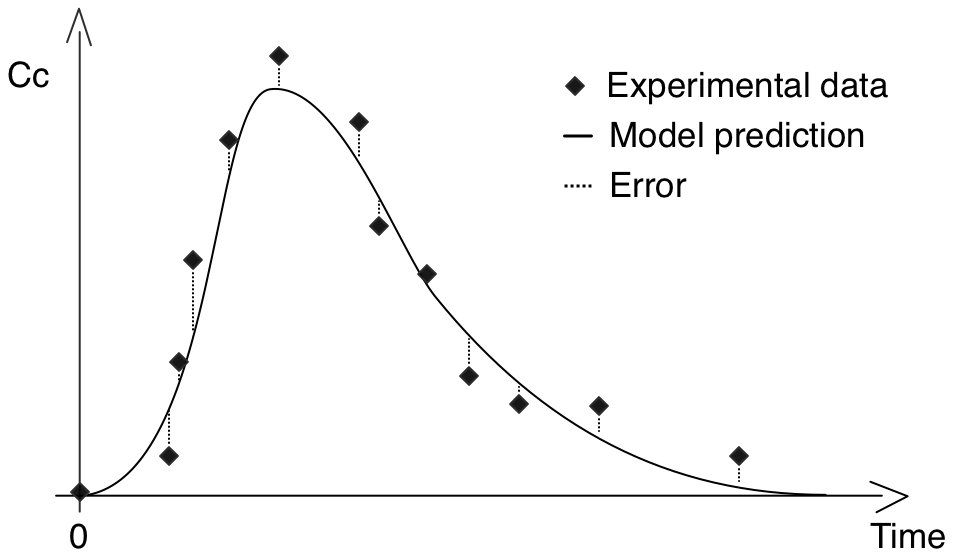
\includegraphics[height=45mm]{Model_individual}
\caption{Frequently sampled individual PK data. The black diamonds stand for experimental data, the solid line for the time course of concentration as predicted by a mathematical model. }
%\caption{Basic mathematical model for frequently sampled individual data. The black diamonds stand for experimental data, the solid line for the time course of concentration as predicted by a mathematical model.}
\label{fig:indivModel}
\end{figure}

\begin{figure}[htbp]
\centering
 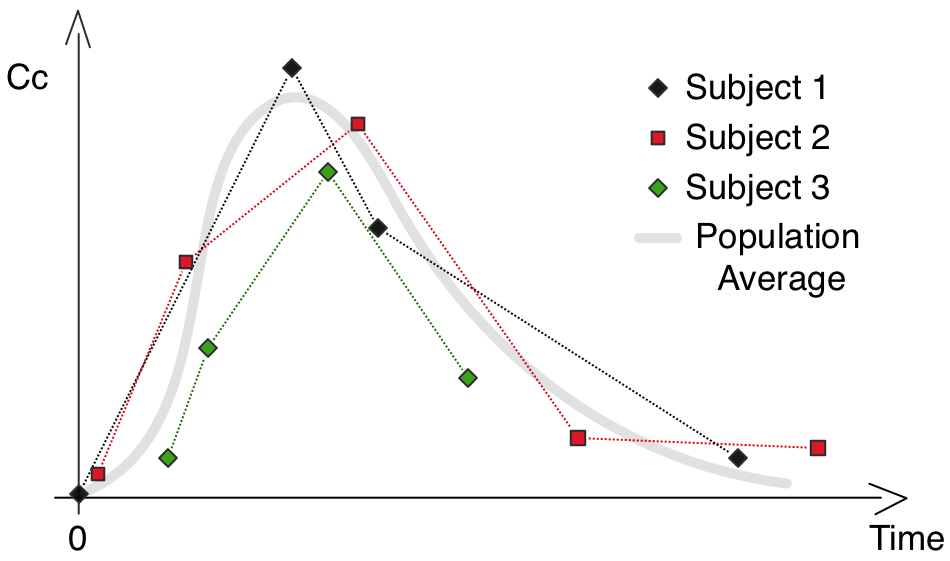
\includegraphics[height=45mm]{Model_population}
\caption{Population PK data --  for three subjects with different observation times and varying characteristics, such as area under the curve, maximum values, time of the maximum etc. The grey line of the population average is to be estimated along with individual estimates.}
%\caption{Basic mathematical model for frequently sampled individual data. The black diamonds stand for experimental data, the solid line for the time course of concentration as predicted by a mathematical model.}
\label{fig:popModel}
\end{figure}

\section{Non-linear mixed effect models}

The approach which proved to be very effective for the analysis of population data is that of \textbf{nonlinear mixed effect models}, NLME. The nonlinearity means that it can handle virtually any type of structural model, usually highly non-linear. Additionally one can consider population or subject related factors, known \emph{a priori} or collected during the study, which can be divided into two groups:
\begin{itemize}
\item
\textbf{fixed effects} -- population averages, e.g. typical/population value for volume, and other group or even subject specific explanatory variables, such as treatment groups, gender or weight, see covariate model in section \ref{maths:covariate_model}.
\item
\textbf{random effects} -- subject/occasion specific, e.g. \textit{inter-individual} or \textit{inter-individual within subject within centre variability}, see section \ref{sec:variabilityModel} on variability.
\end{itemize}
The notation of fixed versus random effects might be at first confusing as the former account for population, group but also subject characteristics. As explained in the parameter model section, the values of individual characteristics are subject specific features but the parameters assigned to them are identical for a group or population. \\
The structure of this chapter is the following, in section \ref{sec:continuousDataModel} we formulate a general nonlinear mixed effects model for continuous data, section \ref{sec:structuralModel} introduces the structural model, section \ref{sec:variabilityModel} discusses the variability as nested hierarchy, section \ref{sec:parameterModel} is about the parameter model, with discussion on correlation of random effects, covariate model and a comparison of equivalent representations of the parameter model and section \ref{sec:residualErrorModel} is about the residual error model. 
% and last section \ref{sec:CTS} about the trial design model.


\section{Continuous data model}
\label{sec:continuousDataModel}
A general nonlinear mixed effects model for continuous data for $N$ subjects and $n_i$ measurements per subject $i$ reads as follows (\cite{Lavielle:2012b}):
\begin{align}
 \underbrace{ y_{ij}}_{\text{\parbox{2cm}{\centering Experimental \\[-4pt]  data}}} =
 \underbrace{ f(x_{ij}, \psi_{i})}_{\text{\parbox{2.5cm}{\centering Model \\[-4pt]  prediction}}} + 
 \underbrace{ g(x_{ij}, \psi_{i}, \xi) \; \epsilon_{ij}}_{\text{\parbox{3cm}{\centering Error}}} 
\quad 1\le i \le N, \quad 1\le j \le n_i \label{eq:nlmeModel}
 \end{align}
with
\begin{itemize}
\item
$y_{ij}$ -- $j^{th}$ observation for subject $i$
\item
$f$ -- structural model prediction
\item
$x_{ij}$ -- regression variables, e.g. $time$ or $concentration$
\item
$\psi_{i}$ -- individual parameters
\item
$\epsilon_{ij}$ -- residual error
\item
$g$ -- standard deviation of the residual error
\item 
$\xi$ -- parameters of the residual model
\end{itemize}
With $\epsilon_{ij}$ being normal distributed with mean 0 and variance 1, $y_{ij}$ is also normally distributed with mean $ f(x_{ij}, \psi_{i})$ and the standard deviation $g(x_{ij}, \psi_{i}, \xi)$. 


\section{Structural model}
\label{sec:structuralModel}
This section deals with the first term of the right hand side in eq.\ref{eq:nlmeModel}
\begin{align*}
	f(x_{ij}, \psi_{i}) 
\end{align*}
i.e. the model prediction.

It can be formulated as a simple algebraic equation (e.g. Hill equation) or complex physiology-based PK model implemented as system of ODEs. When defined in such framework, this deterministic model for an individual will later be embedded in a statistical model. Other approaches, such as SDE-based structural models are not supported in this specification.

%\begin{figure}[htbp]
%\begin{center}
%\includegraphics[width=.45\textwidth]{CTS1_smallPKPD}
%\caption{Simulated combined model as defined in the example with PK (blue) and PD (green) time courses for one subject. Here three doses were administered every $48h$.}
%\label{fig:simplePKPD}
%\vspace{-20pt}
%\end{center}
%\end{figure}
%  \vspace{-20pt}
%  \caption{A gull}
%  \vspace{-10pt}
%\end{wrapfigure}
\paragraph{Example}
As an example of a structural model we consider a combined PK/PD model, % see figure \ref{fig:simplePKPD},
\begin{itemize}
\item
PK -- oral one-compartmental model
\item
PD -- turnover model, so called $I_{max}$ model
\end{itemize}
with the following model parameters $ka$, $V$, $CL$, $Imax$, $IC50$, $Rin$ and $kout$.
\begin{align*}
k&=CL/V  \\
\frac{dAd}{dt} &=-ka\times Ad  \\
\frac{dAc}{dt}&=ka \times Ad - k \times Ac  \\
\frac{dE}{dt}&=Rin \times \Bigg(1-\frac{Imax \times Cc}{Cc+IC50}\Bigg) - kout \times E \\
\mbox{Initial condition: } & E(t=0) = Rin/kout   \\
& Ad(t=0) = DoseSize  \\
& Ac(t=0) = 0;  \\
Cc &= Ac/V  
\end{align*}

\paragraph{Alternative formulation}
The PK model can, in this case, be formulated as an algebraic equation because an analytic solution exists, i.e.
\begin{align*}
C(t) = \frac{D}{V}  \frac{ka}{ka - k} \Big(e^{-k(t-t_D)} - e^{-ka(t-t_D)} \Big) 
\end{align*}


%
%\begin{eqnarray}
%\frac{d\textbf{y}(t)}{dt} &=& F(t,\textbf{y}(t)) \nonumber \\
%with  && \textbf{y}(t_0) = \textbf{y}_0  \nonumber
%\end{eqnarray}
%
%i.e. using explicit, first order ODEs.
%
%\paragraph*{Note on initial conditions}
%Some models have long algebraic expressions for every initial condition, e.g. here the value for glucose in liver:
%\begin{eqnarray}
%G_{L,0}=(1/Q_{G,L})*(Q_{G,A}*G_{H,0} + Q_{G,G}*G_{G,0} + Q_{G,PN}*G_{PN,0} + r_{B_{HGP}} - r_{B_{HGU}}) \nonumber
%\end{eqnarray}
%with 
%Initial conditions (defined/calculated before)
%\begin{eqnarray}
%&&G_{H,0} = a; \;\;\;G_{G,0} = b; \;\;\;G_{PN,0} = c; \quad with \quad a,b,c \in R \nonumber 
%\end{eqnarray}
%and other user defined functions
%\begin{eqnarray}
%&& r_{B_{HGP}} = f_1(y) \nonumber \\
%&& r_{B_{HGU}} = f_2(y) \nonumber
%\end{eqnarray}



\section{Nested hierarchy as the random variability structure}
\label{sec:variabilityModel}
\label{math:variability}

This section describes the variability structure of the random effects and the related naming convention. It is largely based on the discussions and conclusions from the Copenhagen focus meeting \cite{Copenhagen:2013}. Accordingly, in the following we will distinguish: 
\begin{itemize}
\item
(related to the observations) -- \textit{residual variability}, also known as \textit{intra-individual variability} and
\item
(related to the parameters) -- \textit{inter-individual} and \textit{inter-occasion variabilities}
\end{itemize}
The former is described in the section \ref{sec:residualErrorModel}, while the latter is described in this section.

\begin{figure}[htb!]
\centering
  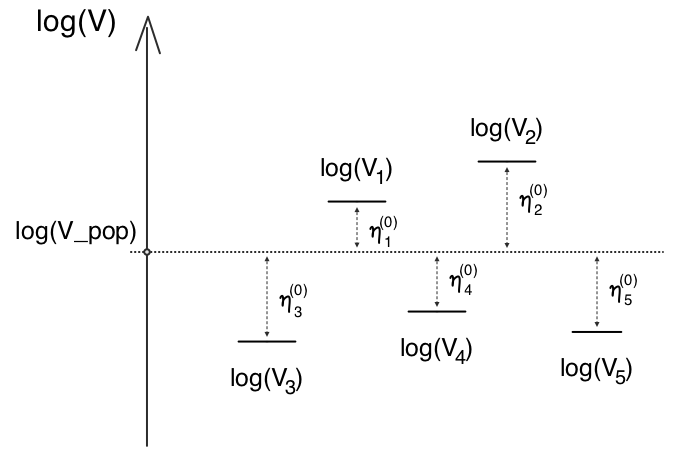
\includegraphics[width=70mm]{Subject-level}
 \caption{Inter-individual variability typically occurring in an experiment, here $\log(V_{i=1\cdots5})$ i.e. values for five subjects, varying around a typical value $\log(V_{pop})$, are shown.}
 \label{fig:subjectLevelVariability}
\end{figure}

\begin{figure}[htb!]
\centering
  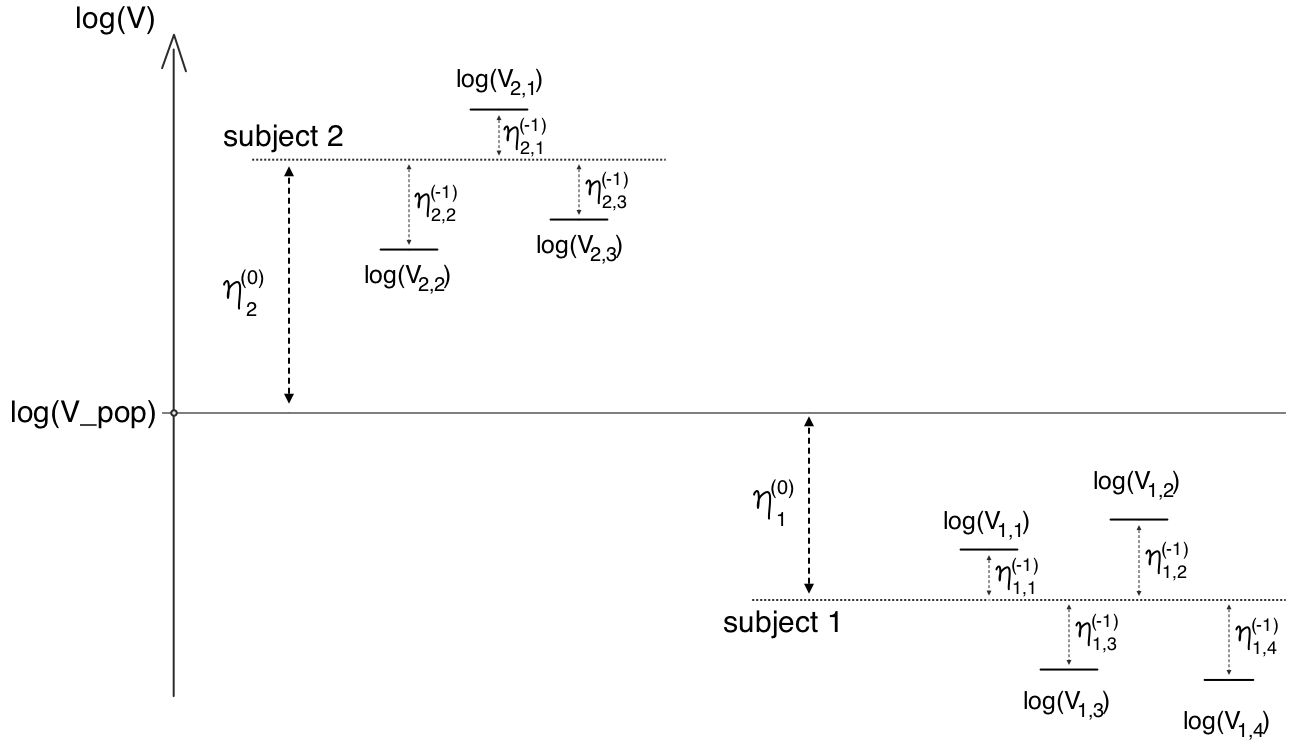
\includegraphics[width=120mm]{Subject-occasion-level}
 \caption{Subject variability level, $(0)$, and within-subject (or occasion) variability level, $(-1)$, typically occurring in an experiment, with index $i$ for subjects and $k$ for occasion. Here two subjects only are visualised, each of them having four or three occasions, respectively.}
 \label{fig:subjectOccasionLevelVariability}
\end{figure}

\subsection{Motivation}
One way to look at variability is to consider the following simple experiment: in this experiment, we estimate the volume of distribution in five subjects. Following a drug administration we collect blood samples over a time interval and estimate each subject's PK parameters. The result will be a set of five individual estimates such as those in Figure \ref{fig:subjectLevelVariability}. The values vary around a certain typical/population value. It is apparent that the only variability source is the fact that these are different persons, i.e. we have a rough estimate of the so called \textit{inter-individual} variability.\\
As an extension of this setup, we can now consider different number of occasions, when the PK parameters are estimated for each subject. If we restrict the discussion to two subjects only, each of them having three or four occasions, respectively, we can illustrate the results such those in Figure \ref{fig:subjectOccasionLevelVariability}. Repeatedly performing the same experiment for each subject is equivalent to create an additional level of variability, the \textit{inter-occasion within individual} variability.\\ 
Similarly, one can add e.g. 'country' as a new variability level. If a clinical trial has been conducted in various countries, it is reasonable to ask if the geographic location influences the outcome of the study. 

\subsection{General case}
As a generalisation of the examples described above, one can derive the \textit{nested hierarchy} (also known as \textit{inclusion hierarchy}) of the variability structure of random effects. It can be visualised as a tree or alternatively using a Venn diagram, see Figures \ref{IOVgeneral_tree}, \ref{IOVgeneral_venn}. \\
The tree representation consists of \textit{nodes} and \textit{links} or \textit{edges}. It has the advantage that it visualises the whole structure explicitly from the top level, the \textit{root} node, down to lowest level of the variability. It provides immediate insights needed to understand or to verify the setup of a trial design. However, in case of a very complex structure, with high number of levels and/or subjects, it can become very large, making the tree difficult to represent in a typical document. It this case showing only partial branches will be more helpful, e.g. Figure \ref{IOVgeneral_tree}. On the contrary, the Venn diagram visualises the levels only, and it might be more suited for the complex cases. Usually, the variability structure consists of only one or two levels, e.g. \textit{individual} or  \{\textit{individual}, \textit{occasion}\}, see examples below. 


The \textit{root}, i.e. the top node in the tree structure, stands for the population/typical value of a parameter. Following the current nomenclature, every subsequent variability level is either 'positive' or 'negative' dependent on its position relative to the 'subject level', denoted as 0 -- the level 'zero'. Each level has a covariance matrix associated with it, i.e. 
\begin{itemize}
\item 
$\Omega^{+n}$ -- for levels above the 'zero' level -- their names will vary according to the nature of the levels. For example the variability on country level is called 'between-country variability'.
\item 
$\Omega^0$ -- also called BSV (between subject variability) or IIV (inter-individual variability).
\item 
$\Omega^{-n}$ -- for levels below the 'zero' level -- called WSV (within-subject variability) or IOV (inter-occasion variability).
\end{itemize}
The number of levels will vary dependent on the nature of the study. Cases without or with only positive/negative levels are possible. Please note that \pharmml doesn't require or use numbers to be assigned to the various levels of variability. Instead the user can define meaningful identifiers.

\begin{figure}[htb!]
\centering
  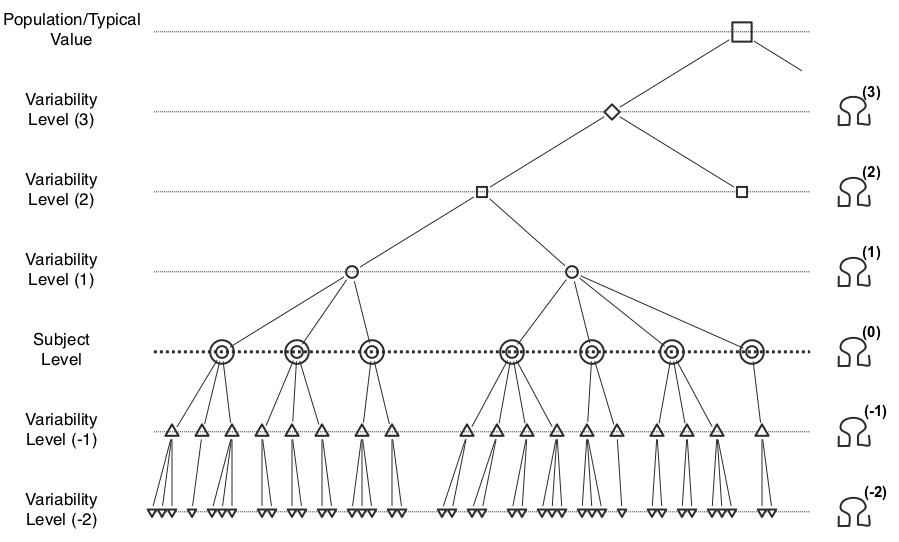
\includegraphics[width=120mm]{IOV-general-TREE}
 \caption{General nested hierarchy of the variability structure -- as tree. Note that \pharmml doesn't require or use numbers to be assigned to the various levels of variability. Instead the user can define meaningful identifiers.}
 \label{IOVgeneral_tree}
\end{figure}

\begin{figure}[htb!]
\centering
  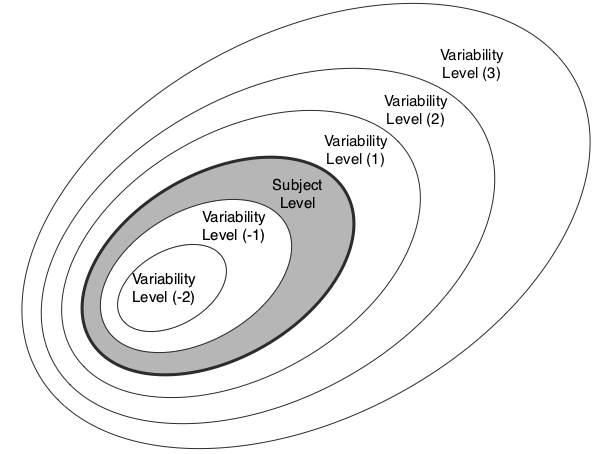
\includegraphics[width=100mm]{IOV-general-VENN}
 \caption{General nested hierarchy of the variability structure -- as Venn diagram.}
 \label{IOVgeneral_venn}
\end{figure}


\paragraph{Example 1}
This example handles the simplest scenario, with only one level of variability: \textit{subject}--level, see Figure \ref{tree_IOV0}. The following symbols are used
\begin{itemize}
\item
$i$ -- subject index, $1\le i \le N$
\end{itemize} 
with $N_l$ -- number of subjects.\\
The typical parameter model, without covariate, reads as follows:
\begin{align*}
& \log(V_i) = \log(V_{pop}) + \eta_i^{(0)}  
\end{align*} 
or alternatively:
\begin{align*}
& V_i = V_{pop} \,e^{\eta_i^{(0)}}  
\end{align*} 
with $\eta_i^{(0)} \sim \mathcal{N}\big(0,\Omega^{(0)}\big)$.


\begin{figure}[htb!]
\centering
  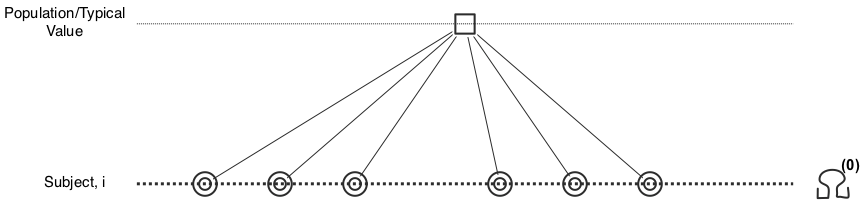
\includegraphics[width=120mm]{tree_IOV0}
 \caption{Example 1 -- single level of variability: \textit{subject}-- level}
 \label{tree_IOV0}
\end{figure}

\paragraph{Example 2}
In this example there are three levels of variability: \{\textit{centre, subject, occasion}\}, see Figure \ref{tree_IOV1}. Following symbols are used:
\begin{itemize}
\item
$l$ -- centre index, $1\le l \le L$
\item
$i$ -- subject index, $1\le i \le N_l$
\item
$k$ -- occasion index, $1\le k \le N_{li}$
\end{itemize} 
with
\begin{itemize}
\item
$L$ -- number of centres
\item
$N_l$ -- number of subjects in centre \textit{l}
\item
$N_{li}$ -- number of occasions in subject \textit{i} in centre \textit{l}
\end{itemize} 
The parameter model, without covariate, reads as follows:
\begin{align*}
& \log(V_{lik}) = \log(V_{pop}) + \eta_l^{(1)} + \eta_{li}^{(0)} + \eta_{lik}^{(-1)}  
\end{align*} 
or alternatively:
\begin{align*}
& V_{lik} = V_{pop} \, e^{\eta_l^{(1)}} e^{\eta_{li}^{(0)}} e^{\eta_{lik}^{(-1)}}  
\end{align*} 
with
\begin{align*}
 & \eta_l^{(1)} \sim \mathcal{N}\big(0,\Omega^{(1)}\big), \quad \eta_{li}^{(0)} \sim \mathcal{N}\big(0,\Omega^{(0)}\big),
\quad \eta_{lik}^{(-1)} \sim \mathcal{N}\big(0,\Omega^{(-1)}\big) 
\end{align*}


\begin{figure}[htb!]
\centering
  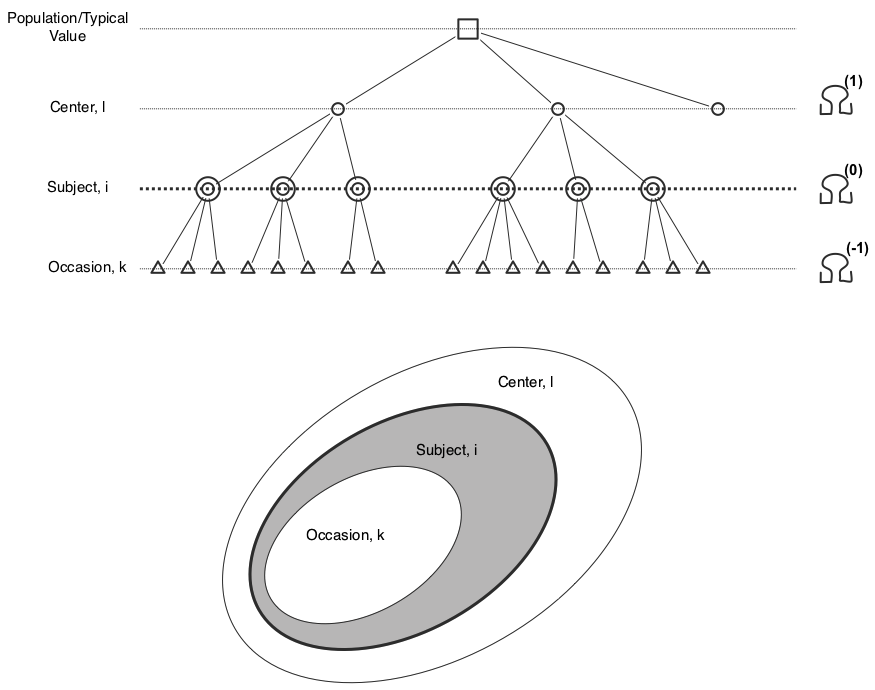
\includegraphics[width=120mm]{tree_IOV1}
 \caption{Example 1 -- three levels of variability: \{\textit{centre, subject, occasion}\}}
 \label{tree_IOV1}
\end{figure}


\paragraph{Example 3}
In this example there are four levels of variability: \{\textit{country, centre, subject, occasion}\}, see Figure \ref{tree_IOV2}. The symbol list is extended by one for 'country' as follows:
\begin{itemize}
\item
$m$ -- country index, $1\le m \le M$
\item
$l$ -- centre index, $1\le l \le N_m$
\item
$i$ -- subject index, $1\le i \le N_{ml}$
\item
$k$ -- occasion index, $1\le k \le N_{mli}$
\end{itemize} 
with
\begin{itemize}
\item
$M$ -- number of countries
\item
$N_m$ -- number of centres in country \textit{m}
\item
$N_{ml}$ -- number of subjects in centre \textit{l} in country \textit{m}
\item
$N_{mli}$ -- number of occasions in subject \textit{i} in centre \textit{l} in country \textit{m}
\end{itemize} 
The parameter model reads as follows:
\begin{align*}
& \log(V_{mlik}) = \log(V_{pop}) + \eta_m^{(2)} + \eta_{ml}^{(1)} + \eta_{mli}^{(0)} + \eta_{mlik}^{(-1)}  
\end{align*} 
or alternatively:
\begin{align*}
& V_{mlik} = V_{pop} \, e^{\eta_m^{(2)}} e^{\eta_{ml}^{(1)}} \; e^{\eta_{mli}^{(0)}} \; e^{\eta_{mlik}^{(-1)}}  
\end{align*} 
with
\begin{align*}
 & \eta_m^{(2)} \sim \mathcal{N}\big(0,\Omega^{(2)}\big), \quad \eta_{ml}^{(1)} \sim \mathcal{N}\big(0,\Omega^{(1)}\big), \quad
 \eta_{mli}^{(0)} \sim \mathcal{N}\big(0,\Omega^{(0)}\big), \quad \eta_{mlik}^{(-1)} \sim \mathcal{N}\big(0,\Omega^{(-1)}\big) 
\end{align*} 



\begin{figure}[htb!]
\centering
  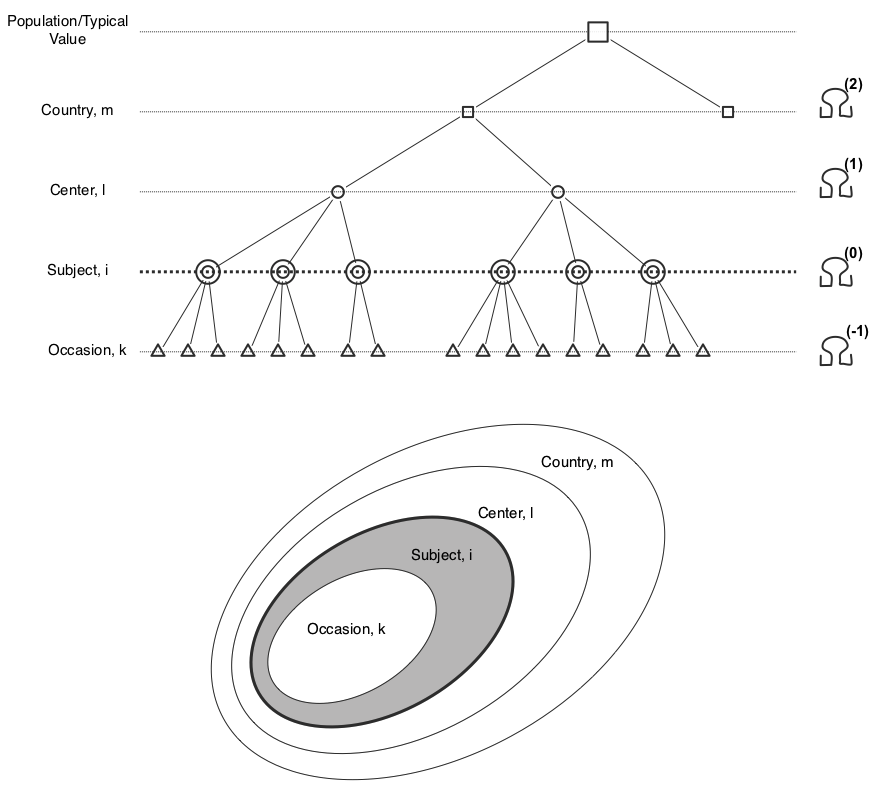
\includegraphics[width=120mm]{tree_IOV2}
 \caption{Example 2 -- four levels of variability:  \{\textit{country, centre, subject, occasion}\}}
 \label{tree_IOV2}
 \end{figure}



\section{Parameter model}
\label{sec:parameterModel}
\label{maths:parameter_defn}
\label{maths:parameter-model}

The following section outlines the parameter model. We consider three types of parameter model:
\begin{itemize}
\item
Type 1. Equation type
\begin{align*}
\psi_i = H(\beta, C_i, \eta_i)
\end{align*}
This is the most general form of a parameter model with no constraints on the function $H$.
It is an implicit equation as it doesn't allow an easy interpretation of its elements in contrast to the two following forms.
\item
Type 2. Gaussian model with general covariate model
\begin{align*}
h(\psi_i) = H(\beta, C_i) + \eta_i
\end{align*}
Here the parameter is normally distributed up to a transformation $h$ with a general covariate model and additive random effects.
\item
Type 3. Gaussian model with linear covariate model
\begin{align*}
h(\psi_i) = h(\psi_{pop}) + \beta \, C_i + \eta_i
\end{align*}
This is a special case of the models above which allows for the most detailed interpretation as explained in the following section.
\end{itemize}
with
\begin{itemize}
\item
$\psi_i$ -- individual parameter
\item
$\psi_{pop}$ -- typical or population mean parameter
\item
$\eta_i$ -- random effect(s)
\item
$\beta$ -- fixed effect(s)
\item
$C_i$ -- covariate(s)
\item
H -- arbitrary function
\item
h -- function which transforms the model on both sides, e.g. log, logit, probit.
\end{itemize}

\subsection{Discussion and examples of Type 1 models}
\label{subsec:paramModelType1}
This model type is the most flexible one, able to accommodate
\begin{itemize}
\item
multiple fixed effects
\item
multiple random effects and
\item
an arbitrary (nonlinear) covariate model.
\end{itemize}

\paragraph{Example}
Let's consider a complex clearance model as introduced in \cite{NONMEM:2006aa}, which contains
\begin{itemize}
\item
four fixed effects $\theta_1, \cdots, \theta_4$
\item
three continuous covariates $WT, AGE, SECR$
\item
one categorical covariate $ICU$
\item
three random effects $\eta_{1i,met}\sim \mathcal{N}(0,\omega_{1,met}^2),\eta_{2i,met}\sim \mathcal{N}(0,\omega_{2,met}^2), \eta_{3i,ren}\sim \mathcal{N}(0,\omega_{3,ren}^2)$
\end{itemize}
The model is composed of
\begin{enumerate}
\item
the average metabolic clearance which reads
\begin{align*}
& CL_{met_{average}} = WT\times \frac{\theta_1 - \theta_2 \times Cpss_2}{\theta_3 + Cpss_2}
\end{align*}
extended with random effects representing a patient being from an ICU (intensive care unit) or else
\begin{align*}
& CL_{i,met} = CL_{met_{average}} + (1 - ICU) \; \eta_{1,i} + ICU \; \eta_{2,i}
\end{align*}
i.e.
\begin{align*}
& CL_{i,met} = \left\{ \begin{array}{lcl}  CL_{met_{average}} + \eta_{1,i}  & \mbox{for} & ICU = 0 \quad \text{i.e. patient not from ICU} \\
CL_{met_{average}} + \eta_{2,i}  & \mbox{for} & ICU = 1 \quad \text{else}
\end{array}\right.
\end{align*}
\item
and average renal clearance which reads
\begin{align*}
& CL_{ren_{average}} = \theta_4 \times RF \quad \text{with}  \quad
RF = WT\times \frac{1.66 - 0.011 \times AGE}{SECR}
\end{align*}
so the clearance for subject $i$ amounts to
\begin{align*}
& CL_{i,ren} = CL_{ren_{average}}(1+ \eta_{3,i})
\end{align*}
\end{enumerate}
The complete model, combining (1) and (2), for an individual's clearance then reads
\begin{align*}
& CL_i = CL_{i,met} + CL_{i,ren}.
\end{align*}
This model, although fully flexible, is difficult to break into meaningful sub-components. This is an entirely different situation for the following model types, where clearly defined sub-components can be separately stored and annotated.
%\begin{itemize}
%\item
%metabolic clearance
%\begin{align*}
%& CL_{met_{average}} = WT\times \frac{\theta_1 - \theta_2 \times Cpss_2}{\theta_3 + Cpss_2}
%\end{align*}
%extended with random effects representing a patient being from an ICU (Intensive Care Unit) or else
%\begin{align*}
%& CL_{met} = CL_{met_{average}} + (1 - ICU) \, \eta_{1i,met} + ICU \, \eta_{2i,met}
%\end{align*}
%i.e.
%\begin{align*}
%& CL_{met} = \left\{ \begin{array}{lcl}  CL_{met_{average}} + \eta_1  & \mbox{for} & ICU = 0 \quad \text{i.e. patient not from ICU} \\
%CL_{met_{average}} + \eta_2  & \mbox{for} & ICU = 1 \quad \text{else}
%\end{array}\right.
%\end{align*}
%\item
%and renal clearance
%\begin{align*}
% CL_{ren} = \theta_4 \times RF
%\end{align*}
%with
%\begin{align*}
%& RF = WT\times \frac{1.66 - 0.011 \times AGE}{SECR}
%\end{align*}
%with covariates \var{WT}, \var{AGE} and \var{SECR}.
%\end{itemize}
%The complete model for an individual's clearance reads
%\begin{align*}
%& CL_i = CL_{met} + CL_{ren}\; \eta_{3i,ren}.
%\end{align*}

\subsection{Discussion and examples of Type 2 models}
\label{subsec:paramModelType2}
Here, we consider normally distributed parameters, up to a transformation $h$, i.e. normal, log-normal or logit-normally distributed with identity, the natural logarithm or the logit as transformation, respectively.

Compared to the Type 1 parameter model, the Type 2 parameter model has a more structured additive form:
\begin{align*}
h(\psi_i) =
\underbrace{H(\beta, C_i)}_{\text{\parbox{2.5cm}{\centering non-linear covariate\\[-4pt] model}}}
+ \underbrace{\eta_i^{(0)}+ \eta_{ik}^{(-1)} + \dots}_{\text{\parbox{3cm}{\centering IIV and other\\[-4pt] levels of variability}}}
\end{align*}
Accordingly a model for an individual parameter consists of
\begin{itemize}
\item
the left-hand transformation, $h$
\item
a non-linear covariate model, i.e. any function, $H$, of fixed effects, \var{\beta}, and categorical or continuous covariates, $C_i$, e.g. \textit{Sex} or \textit{Weight}, and
\item
random effects, $\eta$, for \textit{inter-individual, inter-occasion} and/or other levels of variability (see section \ref{sec:variabilityModel}).
\end{itemize}

\paragraph{Example}
The following example is taken from the 'Fisher/Shafer NONMEM Workshop', and in NMTRAN code reads
\begin{xmlcode}
	WTE = THETA(1) * WT / (THETA(2)+ WT)
	V = (THETA(3) + WTE) * EXP(ETA(1))
\end{xmlcode}
After taking the logarithm of both sides we get
\begin{align*}
\log(V_i) = \log\Big(\theta_3 + \frac{\theta_1 \times WT_i}{\theta_2 + WT_i}\Big) + \eta_{V,i}.
\end{align*}

\subsection{Discussion and examples of Type 3 models}
\label{subsec:paramModelType3}
Here, we again consider normally distributed parameters, up to a transformation $h$, i.e. normal, log-normal or logit-normally distributed with identity, the natural logarithm or the logit as transformation, respectively.

The Type 3 parameter model has a very convenient fully additive form, which separates all of the sub-components, making it very easy to understand and process:
\begin{align*}
h(X_i) = h(X_{pop})
+ \underbrace{\beta \,C_i}_{\text{\parbox{2cm}{\centering linear covariate\\[-4pt] model}}}
+ \underbrace{\eta_i^{(0)}+ \eta_{ik}^{(-1)} + \dots}_{\text{\parbox{3cm}{\centering IIV and other\\[-4pt] levels of variability}}}
\end{align*}
Accordingly a model for an individual parameter consists of
\begin{itemize}
\item
a parameter transformation, $h$
\item
a typical or population mean value of the parameter, $X_{pop}$
\item
a linear covariate model, $\beta \, C_i$, with
\begin{itemize}
\item
fixed effects, $\beta$, and
\item
categorical or continuous covariates, $C_i$, e.g. \textit{Sex} or \textit{Weight}
\end{itemize}
\item
random effects, $\eta$, for \textit{inter-individual, inter-occasion} and/or other levels of variability (section \ref{sec:variabilityModel}).
\end{itemize}
See Figure \ref{fig:weightAsCovariate} for an example of the linear relationship between a parameter and a continuous covariate and one, \textit{inter-individual}, level of variability.

\paragraph{Example}
Let's consider volume, $V$, as a log-normally distributed parameter with two covariates \textit{Sex} and \textit{Weight} and with three levels of variability as discussed in Example 3 in section \ref{sec:variabilityModel} (see Figure \ref{tree_IOV1}), which can be represented by the equation:
%\begin{align*}
%& \eta_i \sim \mathcal{N}(0,\omega_V); \quad \log( V_i ) = \log( V_{pop} ) + \beta_{V,1} 1_{Sex_i=F} + \beta_{V,2} \log\Big(\frac{W_i}{70}\Big) + \eta_{i,V}
%\end{align*}
\begin{align*}
V_{lik} = V_{pop} e^{\beta_{V,1} 1_{Sex_i=F}} \Big(\frac{W_i}{70}\Big)^{\beta_{V,2}} e^{\eta_{l,V}^{(1)}}  e^{\eta_{li,V}^{(0)}} e^{\eta_{lik,V}^{(-1)}}
\end{align*}
or alternatively as
\begin{align*}
\underbrace{\log(V_{lik})}_{\text{\parbox{2cm}{\centering transformed\\[-4pt] individual value}}} =
\underbrace{\log(V_{pop})}_{\text{\parbox{2cm}{\centering transformed\\[-4pt] typical value}}} +
\underbrace{\beta_{V,1} 1_{Sex_i=F}}_{\text{\parbox{2.2cm}{\centering categorical\\[-4pt] covariate model\\[-4pt] for Sex}}}
+ \underbrace{\beta_{V,2} \log\Big(\frac{W_i}{70}\Big)}_{\text{\parbox{2.2cm}{\centering continuous\\[-4pt] covariate model\\[-4pt] for Weight}}}
+ \underbrace{\eta_{l,V}^{(1)}}_{\text{\parbox{1.8cm}{\centering inter-centre\\[-4pt]  variability}}}
+ \underbrace{\eta_{li,V}^{(0)}}_{\text{\parbox{1.8cm}{\centering inter-individual\\[-4pt] within centre \\[-4pt]  variability}}}
+ \underbrace{\eta_{lik,V}^{(-1)}}_{\text{\parbox{2.2cm}{\centering inter-occasion\\[-4pt] within individual \\[-4pt] within centre \\[-4pt] variability}}}
\end{align*}
with
\begin{align*}
 && \eta_{l,V}^{(1)} \sim \mathcal{N}\big(0,\Omega^{(1)}\big), \quad \eta_{li,V}^{(0)} \sim \mathcal{N}\big(0,\Omega^{(0)}\big),
\quad \eta_{lik,V}^{(-1)} \sim \mathcal{N}\big(0,\Omega^{(-1)}\big).
\end{align*}
The equation for $V_{lik}$ represented in the additive form is clearly easier to understand and one can read out the following information from it:
\begin{itemize}
\item
the parameter transformation, the natural logarithm, $log$
\item
the typical volume, $V_{pop}$
\item
the two linear covariate models, $\beta_{V,1} C_1$ and $\beta_{V,2} C_2$ with
\begin{itemize}
\item
a fixed effect for the categorical covariate, $\beta_{V,1}$
\item
a categorical covariate, $1_{Sex_i=F}$
\item
a fixed effect for the continuous covariate, $\beta_{V,2}$
\item
a continuous covariate, $C_2 = \log(W/W_{pop})$ with $W_{pop}=70$
\end{itemize}
\item
multiple random effects
\begin{itemize}
\item
a random effect above the subject level for \textit{inter-centre} variability, $\eta_{l,V}^{(1)}$
\item
a random effect at the subject level for \textit{inter-individual within centre} variability, $\eta_{li,V}^{(0)}$
\item
a random effect below the subject level for \textit{inter-occasion within individual within centre} variability, $\eta_{lik,V}^{(-1)}$.
\end{itemize}
\end{itemize}


\begin{figure}[htbp]
\centering
 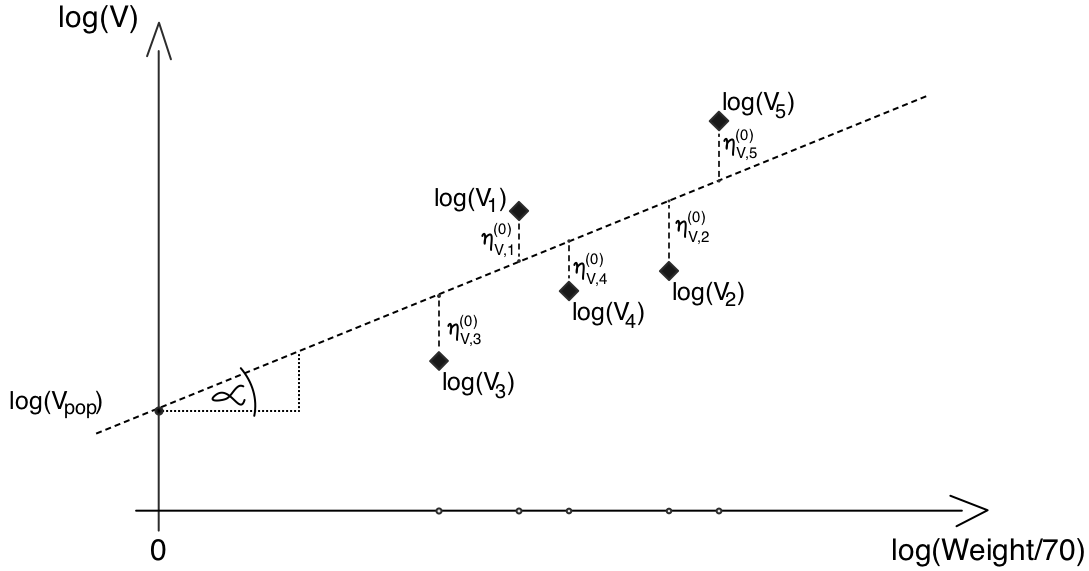
\includegraphics[width=100mm]{weightAsCovariate}
\caption{The linear relationship between the parameter and a continuous covariate after application of appropriate transformations $V_i \longrightarrow \log(V_i)$ and $W \longrightarrow \log(W/70)$ with $\beta_{V,2} = \tan{\alpha}$, the slope of the regression line, and $\log(V_{pop})$ as the $y$-axis intercept.}
\label{fig:weightAsCovariate}
\end{figure}

%%%%%%%%%%%%%%%%%%%%%%%%%%%%%%%%%%%%%%%%%%%%%%%%%%%%%%%%%%%%%%%%%
\subsection{Correlation of random effects}
\label{subsec:correlationModel}\label{maths:param correlation}
Correlation of random effects means that the transformed parameters. e.g. $\log(V_i)$ and $\log(CL_i)$ are correlated as well (although the relationship is not straightforward; see also the discussion below on correlation and covariates). There are two alternative ways to define the correlation, using either
\begin{itemize}
\item
a correlation matrix, $R$, or
\item
a variance-covariance matrix, $\Omega$.
\end{itemize}


\paragraph{Correlation matrix}
In this case it is sufficient to define the non-zero correlation coefficients, e.g. $\rho_{V,CL}$. All other off-diagonal correlation coefficients will be assumed to be equal to 0. For a simple one-compartment oral PK model with parameters $ka$, $V$, $CL$, and a correlation between $CL$ and $V$ the full correlation matrix reads as follows
\[
R =
 \begin{pmatrix}
  1 	& 0 	& 0  	\\
   		& 1	& \rho_{V,CL} \\
  		& 	& 1
 \end{pmatrix}
\]

\paragraph{Variance-covariance matrix}
\label{maths:covariance-mat-derivation}
Alternatively, the variance-covariance matrix for the model
\[
 \Omega =
 \begin{pmatrix}
  \omega_{ka}^2 	& \omega_{ka,V}	& \omega_{ka,CL}\\
   			  	& \omega_{V}^2	& \omega_{V,CL} \\
  				& 				& \omega_{CL}^2
 \end{pmatrix}
 =
  \begin{pmatrix}
  \omega_{ka}^2 	& 0				& 0 \\
   			  	& \omega_{V}^2	& \omega_{V,CL} \\
  				& 				& \omega_{CL}^2
 \end{pmatrix}
\]
is providing the necessary information due to the reletionship
\begin{align*}
	&\mbox{Cov($p_i$,$p_j$)} = \sigma_i \sigma_j \mbox{Corr($p_i$,$p_j$)}  = \sigma_i \sigma_j \;\rho_{i,j} \quad \mbox{i.e.} \quad \omega_{V,CL} = \omega_V \omega_{CL} \rho_{V,CL}
\end{align*}
in which case it is enough to define $\Omega$ to cover the full correlation structure.


%%%%%%%%%%%%%%%%%%%%%%%%%%%%%%%%%%%%%%%%%%%%%%%%%%%%%%%%%%%%%%%%%
\subsection{Covariate model}
\label{maths:covariate_model}

The covariate model accounts for systematic or known subject
characteristics such as treatment group, gender or body
weight. Accordingly, the model can be defined for discrete and
continuous covariates and is the place where one category of fixed
effects is defined (the other being
the population averages, e.g. $V_{pop}$). Of course, the values of
individual characteristics (weight or sex) are subject specific but
the parameters assigned to them are identical for a group or
population.

As described in the example above the contribution of the continuous
covariate $Weight$ to the parameter value is formulated as
$\beta_{V,2} \log(W_i/70)$ (see figure
\ref{fig:weightAsCovariate}). The figure illustrates the linearity
after the appropriate transformation of the parameter, $V_i
\longrightarrow \log(V_i)$ and $W \longrightarrow \log(W/70)$ with
$\beta_{V,2} = \tan{\alpha}$, the slope of the regression line, and
$\log(V_{pop})$ as the $y$-axis intercept.

In the estimation case the values for the covariate are provided for
each individual. In the case of a simulation (see example
\ref{subsec:exp2_TaskDescription}) its probability distribution has to
be estimated. The information we have to provide is summarised in the

\paragraph{Continuous covariate model}
\begin{align*}
Covariates & =  Weight  \\
CovariatesType & = Continuous  \\
CovariatesPopDistribution\{1\} & \sim \mbox{Normal}(pop_{Weight}, \omega_{Weight})  \\
 \text{with} & \quad pop_{Weight}=70.07 \\
 & \quad \omega_{Weight}=14.09  \\
CovariatesTransf & =\log(Weight/70) 
\end{align*}
Analog information has to be provided in the case of a categorical covariate, such as \textit{Sex} and is summarised for a simple example in the

\paragraph{Categorial covariate model}
\begin{align*}
Covariates &= Sex   \\
CovariatesType &= Categorical  \\
CategoriesNumber &= 2   \\
Categories &= \{F,M\}   \\
RefCategory &= F   \\
RefCategProbability &= 14/36 
\end{align*}


%%%%%%%%%%%%%%%%%%%%%%%%%%%%%%%%%%%%%%%%%%%%%%%%%%%%%%%%%%%%%%%%%%%
%%\subsection{Note on correlation and covariates}
%%This section discusses the influence of covariates on correlation between random effects and that of the parameters. In the case without e.g. normally distributed covariates, the correlation is identical. However, the presence of normally distributed body weight in the parameter model has interesting consequences for these correlations. \\
%%Let's consider as an example two correlated log-normally distributed parameters, $V$ and $CL$, without covariates i.e.
%%\begin{align*}
%%& \eta_{V} \sim \mathcal{N}(0,\omega_V); \quad \log( V ) = \log( V_{pop} ) + \eta_{V}  \\
%%& \eta_{CL} \sim \mathcal{N}(0,\omega_{CL}); \quad \log( CL ) = \log( CL_{pop} ) + \eta_{CL}
%%\end{align*}
%%then the correlation between the random effects is identical to the correlation of the (transformed) parameters, see Figure \ref{fig:correlationEtasLogedParams1}.
%%\begin{figure}[h!]
%%\centering
%% 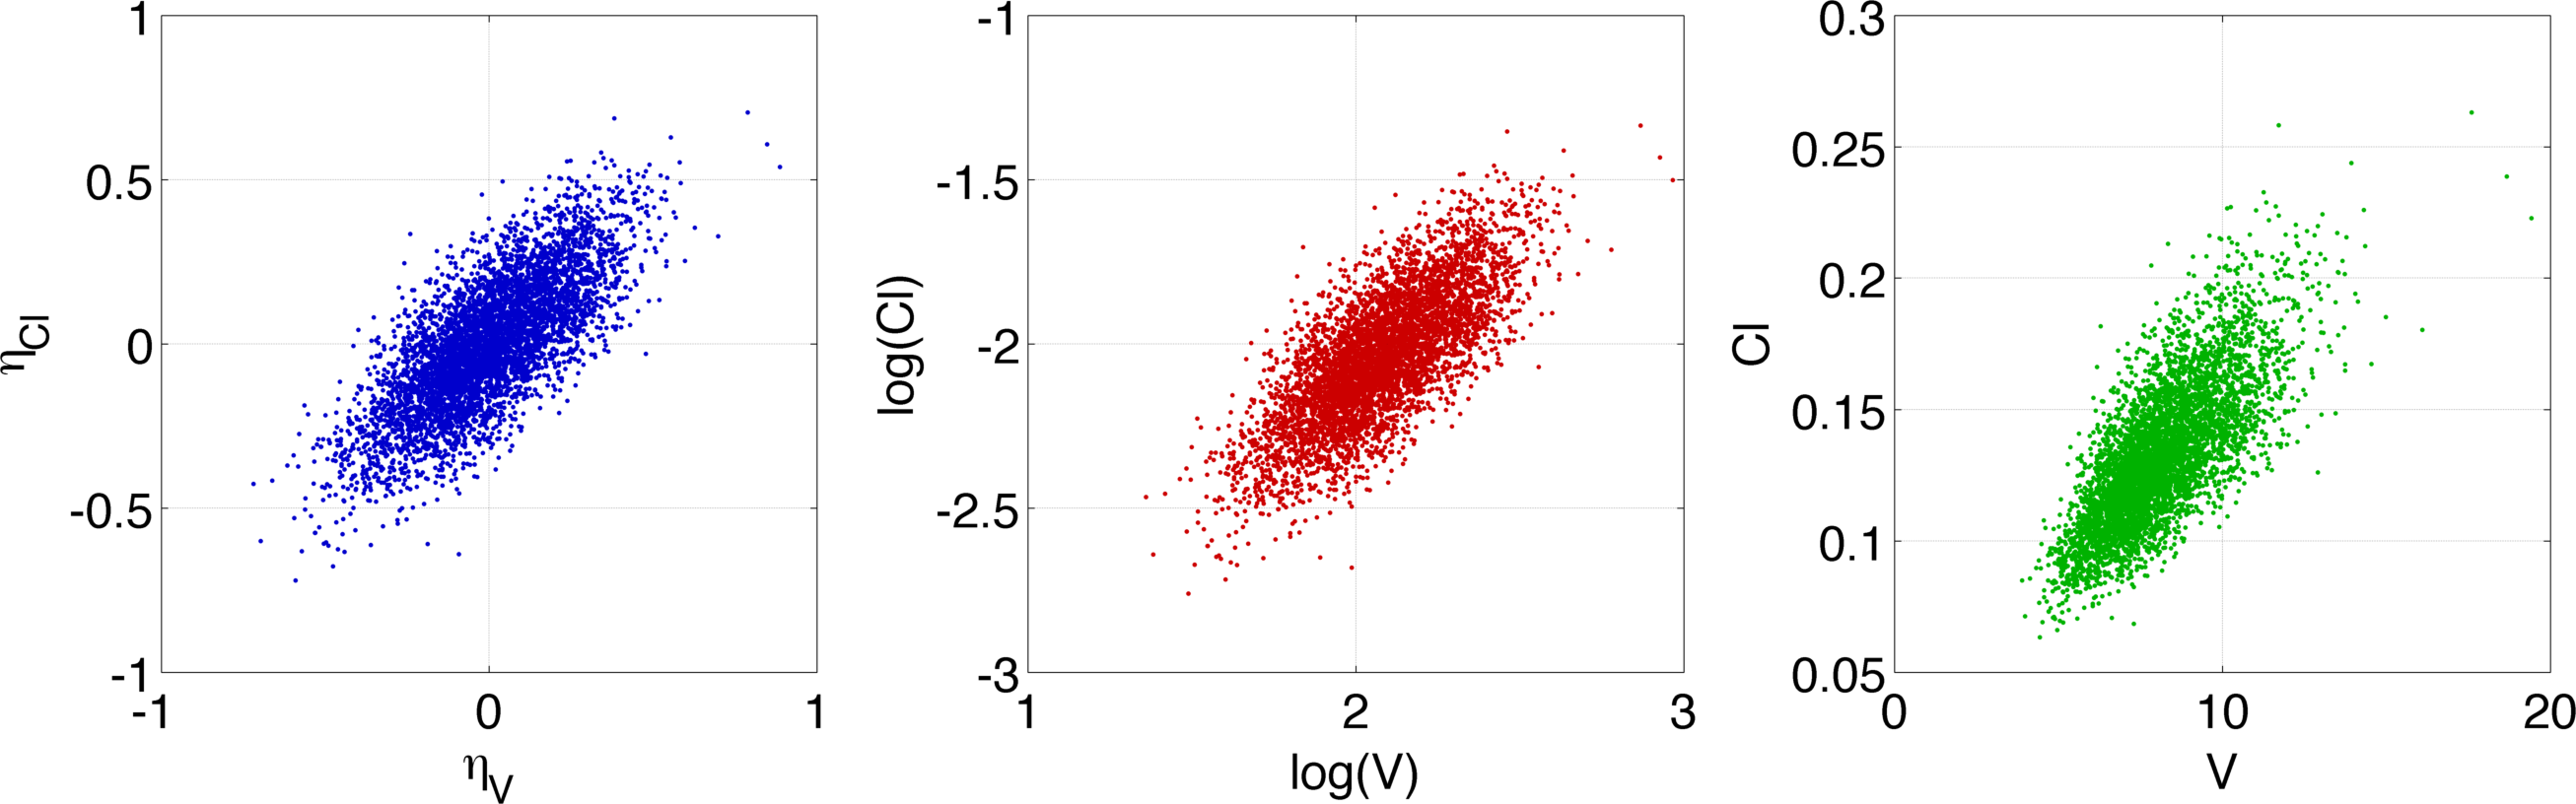
\includegraphics[height=45mm]{correlationsNoCovars}
%%\caption{Correlation of random effects $\eta_V$, $\eta_{CL}$ (blue), transformed parameters $\log(V)$ and $\log(CL)$ (red) and actual parameters  $V$ and $CL$ (green) is equal in the case without covariates. Values used: $V_{pop}=8, \omega_V=0.2, CL_{pop}=0.13,  \omega_{CL}=0.2$.}
%%\label{fig:correlationEtasLogedParams1}
%%\end{figure}
%%\newline
%%Now, we consider that both parameters depend on a continuous normally distributed covariate, e.g. the $Weight$,
%%\begin{align*}
%%& \eta_{V} \sim \mathcal{N}(0,\omega_V); \quad \log( V ) = \log( V_{pop} ) + \beta_{V} \log\Big(\frac{W}{70}\Big) + \eta_{V}  \\
%%& \eta_{CL} \sim \mathcal{N}(0,\omega_{CL}); \quad \log( CL ) = \log( CL_{pop} ) + \beta_{CL} \log\Big(\frac{W}{70}\Big) + \eta_{CL}
%%\end{align*}
%%then the correlation between the transformed parameters is higher then that of the random effects and increases proportionally to $corr(\eta_{V}, \eta_{CL})$, see Figure \ref{fig:correlationEtasLogedParams2}.
%%\begin{figure}[h!]
%%\centering
%% 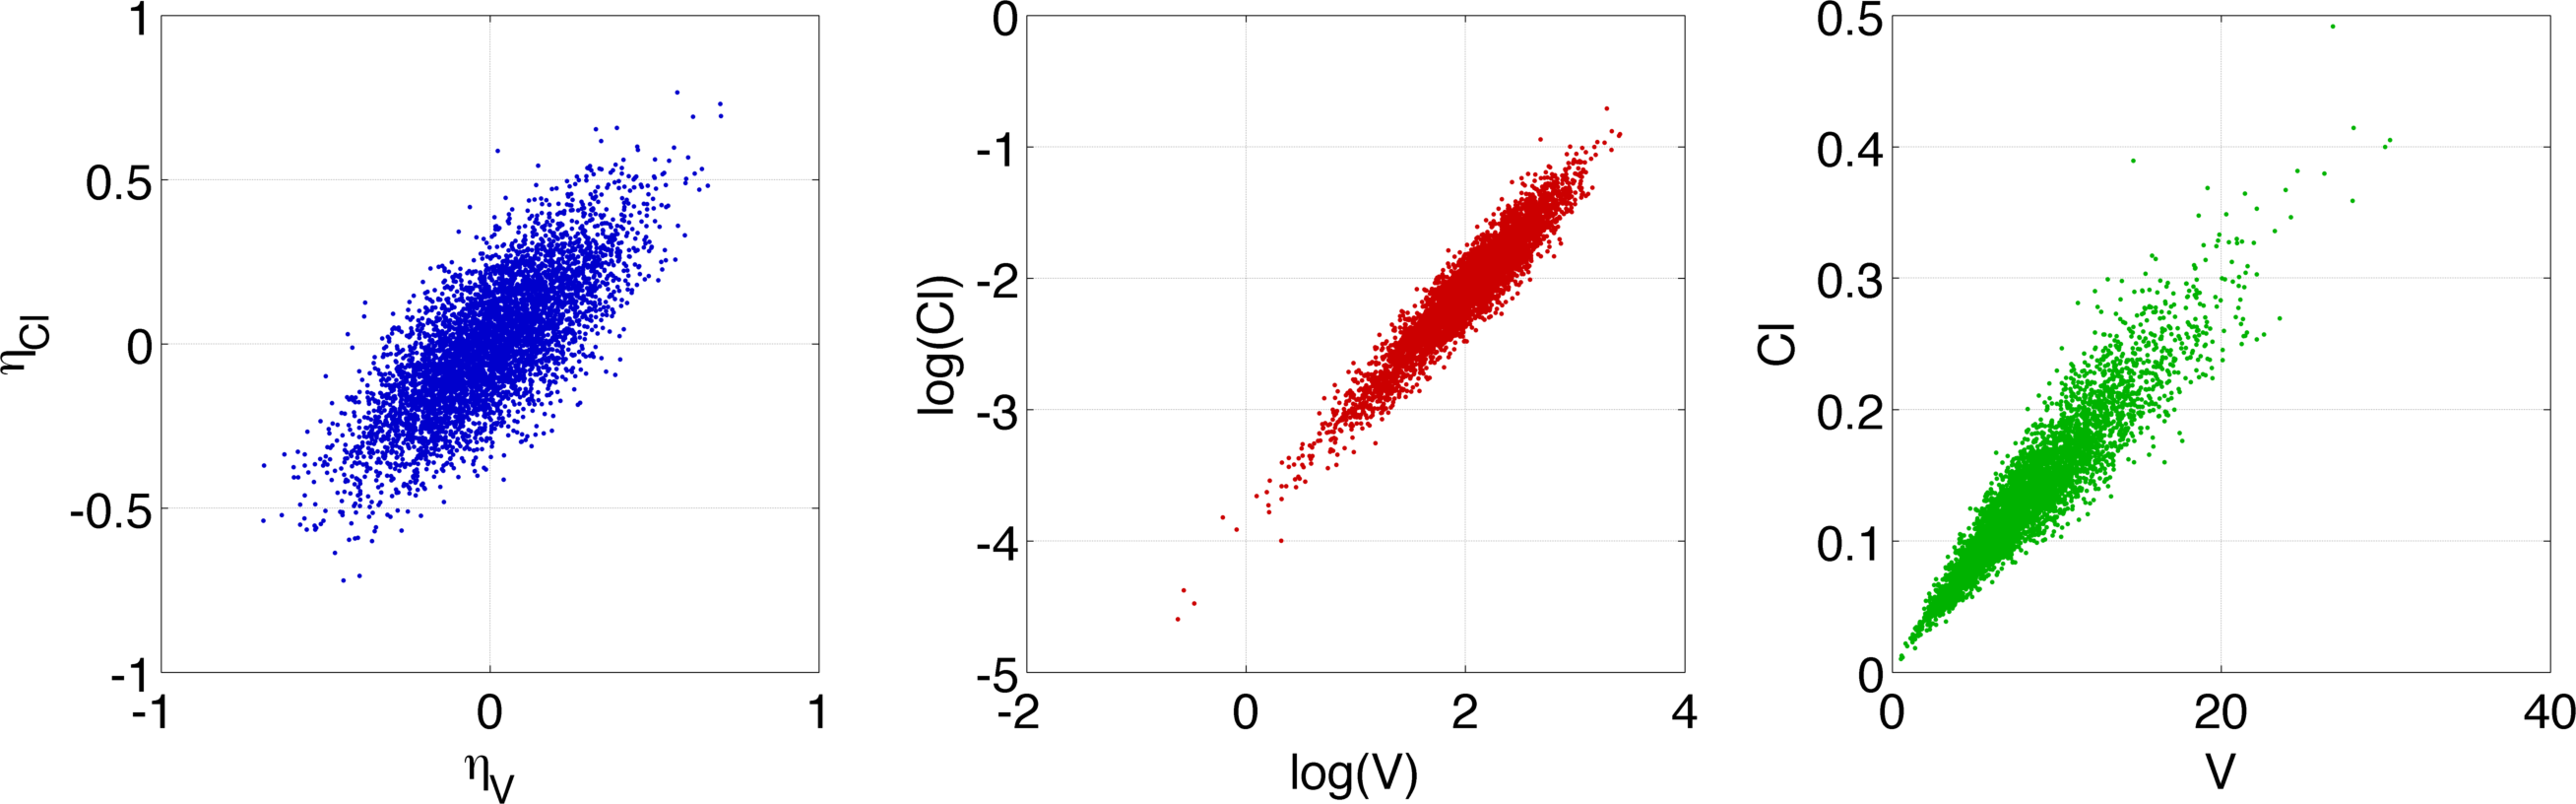
\includegraphics[height=45mm]{correlationsWithCovars}
%%\caption{The correlation between both the transformed parameters (red) and actual parameters (green) is higher then that of the random effects (blue) (and is equal 0.933, 0.948 and 0.750, respectively, for $n=10^8$). Values used as before with $\beta_V=2, \beta_{CL}= 1.75$.}
%%\label{fig:correlationEtasLogedParams2}
%%\end{figure}
%%\newline
%%The consequence of this discussion is that the correlation structure of random effects, as defined in PharmML, translates only in special cases to the correlation between parameters.
%%%This underlines the importance of the fact that we define in PharmML the relationship between random effects and not parameters.


%%%%%%%%%%%%%%%%%%%%%%%%%%%%%%%%%%%%%%%%%%%%%%%%%%%%%%%%%%%%%%%%%
\subsection{Equivalent representations of the parameter model}
Every parameter model represented in the Type 3 format discussed before has at least three mathematically equivalent representation forms,
which will be presented and discussed in terms of advantages and disadvantages in the following. It is important to understand these different
representation forms, as they explain the different forms of notation used in different software tools. Here, we concentrate on NONMEM and MONOLIX only.

%%%%%%%%%%%%%%%%%%%%%%%%%%%%%%%%%%%%%%%%%%%%%%%%%%%%%%%%%%%%%%%%%
% Log-Normal distributed
%%%%%%%%%%%%%%%%%%%%%%%%%%%%%%%%%%%%%%%%%%%%%%%%%%%%%%%%%%%%%%%%%

\subsubsection{Log-Normal distributed}
For a \textbf{log-normal} distributed parameter, e.g. $V$, the equivalent representations read
\begin{align*}
&(1) \eta_i \sim \mathcal{N}(0,\omega_V); \quad V_i= V_{pop} \; e^{\eta_{i,V}}   \\
&(2) \eta_i \sim \mathcal{N}(0,\omega_V); \quad \log( V_i ) = \log( V_{pop} ) + \eta_{i,V}  \\
&(3) \log( V_i ) \sim \mathcal{N}\big( \log( V_{pop} ),\omega_V\big)
\end{align*}
for a typical value $V_{pop}$ and standard deviation $\omega_V$ as described in \cite{Lavielle:2012b}.\\
The typical NMTRAN code for a log-normally distributed parameter is (\cite{Smith:2012aa})
\begin{lstlisting}
GRPV=THETA(1)
V=GRPV*EXP(ETA(1))
\end{lstlisting}
and in MLXTRAN (\cite{MonolixOverview:2012})
\begin{lstlisting}
# as explicit equation
eta_V ~ normal(0, omega_V)
V = V_pop*exp(eta_V)

# or using short notation
V = {distribution=lognormal, typical=V_pop, sd=omega_V}
\end{lstlisting}

\begin{figure}[htbp]
\centering
 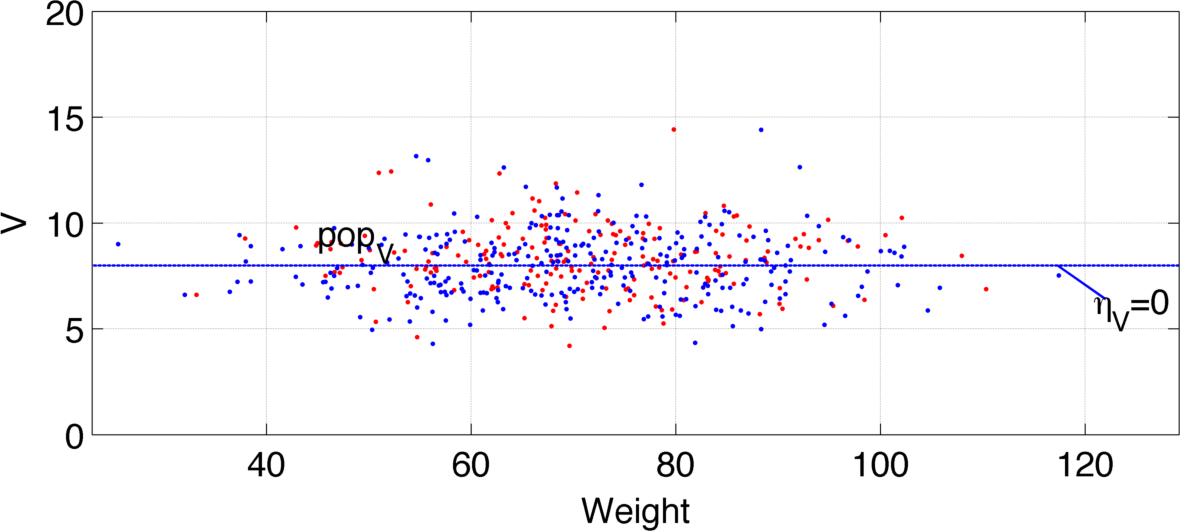
\includegraphics[width=100mm]{paramCovModel_V}
\caption{Log-normally distributed 'V' with $V_{pop}=8$ and $\omega_V=0.2$}
\label{fig:parameterCovModel0}
\end{figure}


%%%%%%%%%%%%%%%%%%%%%%%%%%%%%%%%%%%%%%%%%%%%%%%%%%%%%%%%%%%%%%%%%
% Log-Normal distributed with a continuous covariate
%%%%%%%%%%%%%%%%%%%%%%%%%%%%%%%%%%%%%%%%%%%%%%%%%%%%%%%%%%%%%%%%%

\subsubsection{Log-Normal distributed with a continuous covariate}
For a \textbf{log-normal} distributed parameter, e.g. $V$, with body weight, $W$, as covariate the equivalent representations read
\begin{align*}
& (1) \quad \eta_i \sim \mathcal{N}(0,\omega_V); \quad V_i= V_{pop} \; \big(\frac{W_i}{70}\big)^\beta \; e^{\eta_{i,V}}   \\
&(2) \quad \eta_i \sim \mathcal{N}(0,\omega_V); \quad \log( V_i ) = \log( V_{pop} ) + \beta \log\big(\frac{W_i}{70}\big) + \eta_{i,V}  \\
&(3) \quad \log( V_i ) \sim \mathcal{N}\big( \log( V_{pop} )+ \beta\log\Big(\frac{W_i}{70}\Big),\omega_V\big)
\end{align*}
The typical NMTRAN code for a log-normally distributed parameter with weight as covariate is
\begin{lstlisting}
GRPV=THETA(1)*(WT/70)**THETA(2)
V=GRPV*EXP(ETA(1))
\end{lstlisting}
and in MLXTRAN
\begin{lstlisting}
# as explicit equation
V_pop = V_pop*(weight/70)^beta_V
eta_V ~ normal(0, omega_V)
V = V_pop*exp(eta_V)

# or using short notation
V = {distribution=lognormal, typical=V_pop, covariate=lw70, coefficient=beta_V, sd=omega_V}
\end{lstlisting}
with $lw70 \equiv \log(W/70)$.

\begin{figure}[htbp]
\centering
 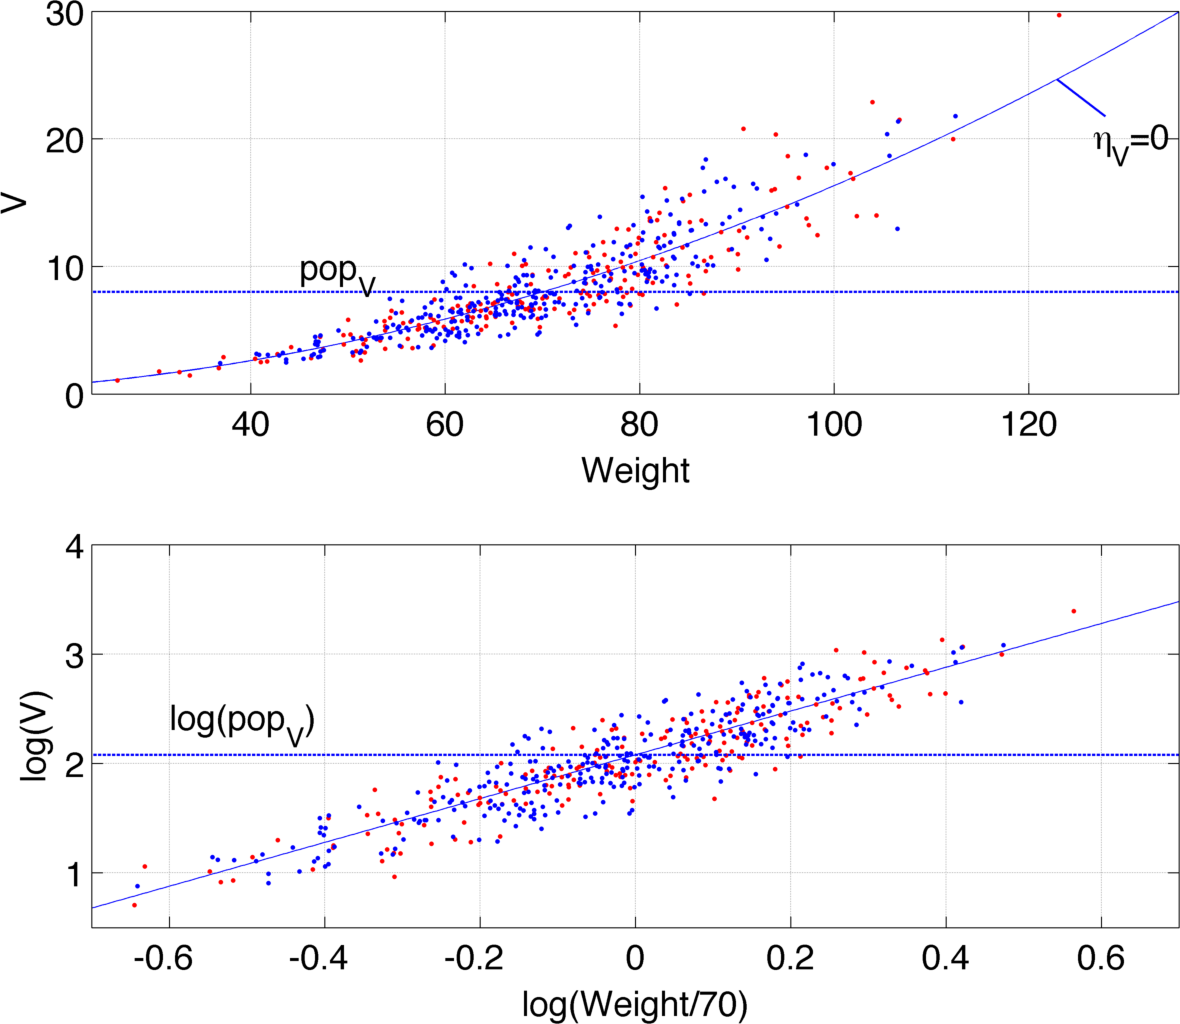
\includegraphics[width=100mm]{paramCovModel_VlogV}
\caption{Log-normally distributed 'V' with 'Weight' as covariates.}
\label{fig:parameterCovModel1}
\end{figure}


%%%%%%%%%%%%%%%%%%%%%%%%%%%%%%%%%%%%%%%%%%%%%%%%%%%%%%%%%%%%%%%%%
% Logit-Normal distributed
%%%%%%%%%%%%%%%%%%%%%%%%%%%%%%%%%%%%%%%%%%%%%%%%%%%%%%%%%%%%%%%%%

\subsubsection{Logit-Normal distributed}
For a \textbf{logit-normal} distributed parameter, e.g. $Imax$, the equivalent representations read
\begin{align*}
&(1) \quad \eta_i \sim \mathcal{N}(0,\omega); \quad  Imax_i= \frac{\bigg[\frac{ Imax_{pop}}{1- Imax_{pop}} \; e^{\eta_{i, Imax}} \bigg]}{ 1+  \bigg[\frac{ Imax_{pop}}{1- Imax_{pop}} \; e^{\eta_{i, Imax}} \bigg]}   \\
&(2) \quad  \eta_i \sim \mathcal{N}(0,\omega); \quad \mbox{logit}(  Imax_i ) = \mbox{logit}(  Imax_{pop} ) + \eta_{i, Imax}  \\
&(3) \quad  \mbox{logit}(  Imax_i ) \sim \mathcal{N}\big( \mbox{logit}( Imax_{pop} ),\omega\big)
\end{align*}
Equation (1) can be rewritten using '$logit$' as follows
\begin{align*}
& Imax_i= \frac{\exp\big(logit(Imax_{pop})  + \eta_{i,Imax} \big)}{ 1+ \exp\big(logit(Imax_{pop}) + \eta_{i,Imax} \big)}  \\
& \Leftrightarrow  Imax_i= \frac{1}{ 1+ \exp\big(- logit(Imax_{pop}) - \eta_{i,Imax} \big)}
\end{align*}\newline
The last form is used for a typical NMTRAN implementation of a logit-normally distributed parameter
\begin{lstlisting}
LGTIMAX=LOG(POP_IMAX/(1-POP_IMAX)) + ETA(IMAX)
IMAX=1/(1+EXP(-LGTIMAX))
\end{lstlisting}
and in MLXTRAN
\begin{lstlisting}
# as explicit equation
eta_Imax ~ normal(0, omega_Imax)
logitImaxi = log(pop_Imax/(1-pop_Imax)) + eta_Imax
Imaxi = 1/(1 + exp(-logitImaxi))

# or using short notation
Imax = {distribution=logitnormal, typical=Imax_pop, sd=omega_Imax}
\end{lstlisting}


%%%%%%%%%%%%%%%%%%%%%%%%%%%%%%%%%%%%%%%%%%%%%%%%%%%%%%%%%%%%%%%%%
% Logit-Normal distributed with a continuous covariate
%%%%%%%%%%%%%%%%%%%%%%%%%%%%%%%%%%%%%%%%%%%%%%%%%%%%%%%%%%%%%%%%%

\subsubsection{Logit-Normal distributed with a continuous covariate}
For a \textbf{logit-normal} distributed parameter with \textit{Weight} as \textbf{covariate} we have
\begin{align*}
&(1)\quad \eta_i \sim \mathcal{N}(0,\omega); \quad Imax_i= \frac{\bigg[\frac{Imax_{pop}}{1-Imax_{pop}} \; \big(\frac{W_i}{70}\big)^\beta \; e^{\eta_{i,Imax}} \bigg]}{ 1+  \bigg[\frac{Imax_{pop}}{1-Imax_{pop}} \; \big(\frac{W_i}{70}\big)^\beta \; e^{\eta_{i,Imax}} \bigg]}
\end{align*}
\begin{align*}
&(2)\quad \eta_i \sim \mathcal{N}(0,\omega); \quad \mbox{logit}( Imax_i ) = \mbox{logit}( Imax_{pop} ) + \beta \log\bigg(\frac{W_i}{70}\bigg) + \eta_{i,Imax}  \\
&(3)\quad \mbox{logit}(  Imax_i ) \sim \mathcal{N}\big( \mbox{logit}( Imax_{pop}) + \beta\log\Big(\frac{W_i}{70}\Big),\omega\big)
\end{align*}
The first equation can be rewritten as follows
\begin{align*}
& Imax_i= \frac{\exp\big(logit(Imax_{pop}) + \beta \log\big(\frac{W_i}{70}\big) + \eta_{i,Imax} \big)}{ 1+ \exp\big(logit(Imax_{pop}) + \beta \log\big(\frac{W_i}{70}\big) + \eta_{i,Imax} \big)}  \\
& \Leftrightarrow Imax_i= \frac{1}{ 1+ \exp\big(- logit(Imax_{pop}) - \beta \log\big(\frac{W_i}{70}\big) - \eta_{i,Imax} \big)}
\end{align*}\newline
The last form is used for a typical NMTRAN implementation of a logit-normally distributed parameter with covariate
\begin{lstlisting}
LGTIMAX=LOG(POP_IMAX/(1-POP_IMAX)) + BETA*LOG(WT/70) + ETA(IMAX)
IMAX=1/(1+EXP(-LGTIMAX))
\end{lstlisting}
and in MLXTRAN
\begin{lstlisting}
# as explicit equation
eta_Imax ~ normal(0, omega_Imax)
logitImaxi = log(pop_Imax/(1-pop_Imax)) + beta*lw70 + eta_Imax
Imaxi = 1/(1 + exp(-logitImaxi))

# or using short notation
Imax =	{distribution=lognormal, typical=Imax_pop, covariate=lw70, coefficient=beta_Imax, sd=omega_Imax}
\end{lstlisting}

\begin{figure}[htbp]
\centering
 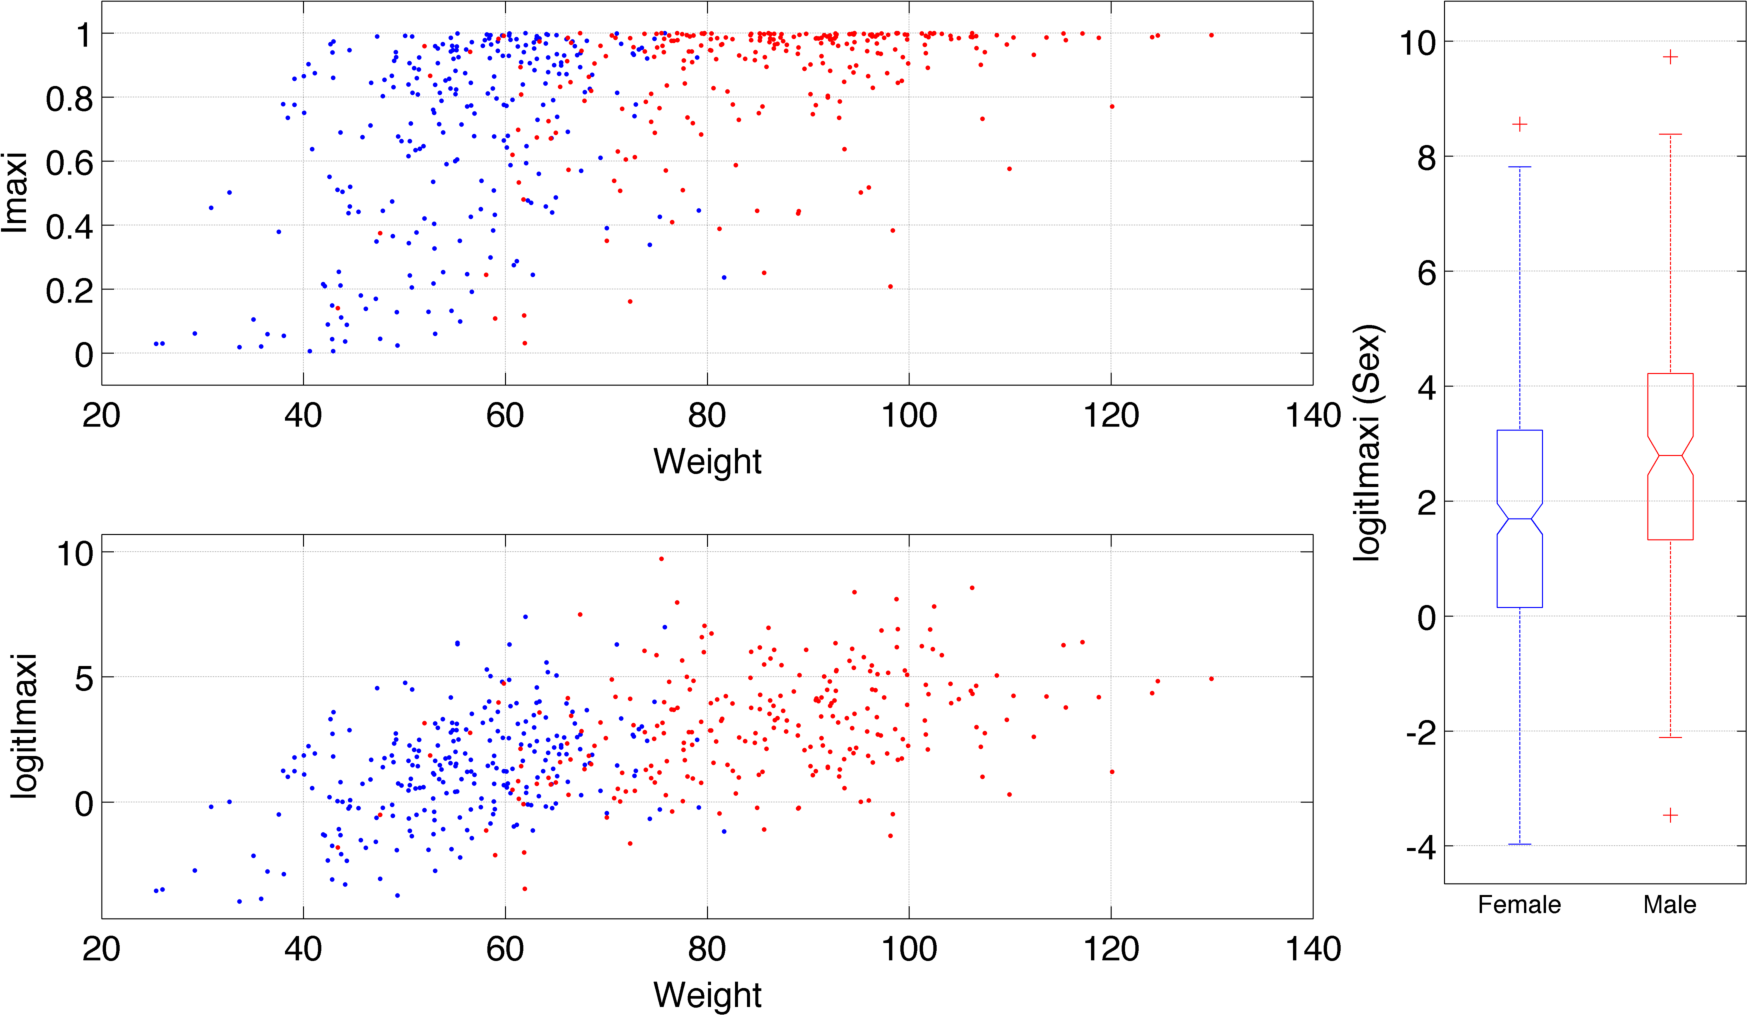
\includegraphics[width=100mm]{paramCovModel_ImaxlogImax_Weight}
\caption{Logit-normally distributed 'Imax' with 'Weight' as covariate.}
\label{fig:parameterCovModel3}
\end{figure}


%%%%%%%%%%%%%%%%%%%%%%%%%%%%%%%%%%%%%%%%%%%%%%%%%%%%%%%%%%%%%%%%%%
%% Logit-Normal distributed with a categorical covariate
%%%%%%%%%%%%%%%%%%%%%%%%%%%%%%%%%%%%%%%%%%%%%%%%%%%%%%%%%%%%%%%%%%
%
%\subsubsection{Logit-Normal distributed with a categorical covariate}
%For a \textbf{logit-normal} distributed parameter with \textit{Sex} as \textbf{covariate} we have
%\begin{align*}
%&(1)\quad \eta_i \sim \mathcal{N}(0,\omega); \quad Imax_i= \frac{\bigg[\frac{Imax_{pop}}{1-Imax_{pop}} \; e^{\beta_{Imax_i} 1_{Sex_i=F}} \; e^{\eta_{i,Imax}} \bigg]}{ 1+  \bigg[\frac{Imax_{pop}}{1-Imax_{pop}} \; e^{\beta_{Imax_i} 1_{Sex_i=F}} \; e^{\eta_{i,Imax}} \bigg]}  \\
%&(2)\quad \eta_i \sim \mathcal{N}(0,\omega); \quad \mbox{logit}( Imax_i ) = \mbox{logit}( Imax_{pop} ) + \beta_{Imax_i} 1_{Sex_i=F} + \eta_{i,Imax}  \\
%&(3)\quad \mbox{logit}(  Imax_i ) \sim \mathcal{N}\big( \mbox{logit}( Imax_{pop}) + \beta_{Imax_i} 1_{Sex_i=F},\omega\big)
%\end{align*}
%The first equation can be rewritten as follows
%\begin{align*}
%& Imax_i= \frac{\exp\big(logit(Imax_{pop}) + \beta_{Imax_i} 1_{Sex_i=F} + \eta_{i,Imax} \big)}{ 1+ \exp\big(logit(Imax_{pop}) + \beta_{Imax_i} 1_{Sex_i=F} + \eta_{i,Imax} \big)}  \\
%& \Leftrightarrow Imax_i= \frac{1}{ 1+ \exp\big(- logit(Imax_{pop}) - \beta_{Imax_i} 1_{Sex_i=F} - \eta_{i,Imax} \big)}
%\end{align*}\newline
%The last form is used for a typical implementation of a logit-normally distributed parameter with covariate:\\
%in NMTRAN
%\begin{lstlisting}
%LGTIMAX=LOG(POP_IMAX/(1-POP_IMAX)) + BETA*SEX + ETA(IMAX)
%IMAX=1/(1+EXP(-LGTIMAX))
%\end{lstlisting}
%and in MLXTRAN
%\begin{lstlisting}
%# as explicit equation
%eta_Imax ~ normal(0, omega_Imax)
%logitImaxi = log(pop_Imax/(1-pop_Imax)) + beta*Sex + eta_Imax
%Imaxi = 1/(1 + exp(-logitImaxi))
%
%# or using short notation
%Imax =	{distribution=lognormal, typical=Imax_pop, covariate=Sex, coefficient=beta_Imax, sd=omega_Imax}
%\end{lstlisting}
%
%
%\begin{figure}[h!]
%\centering
% 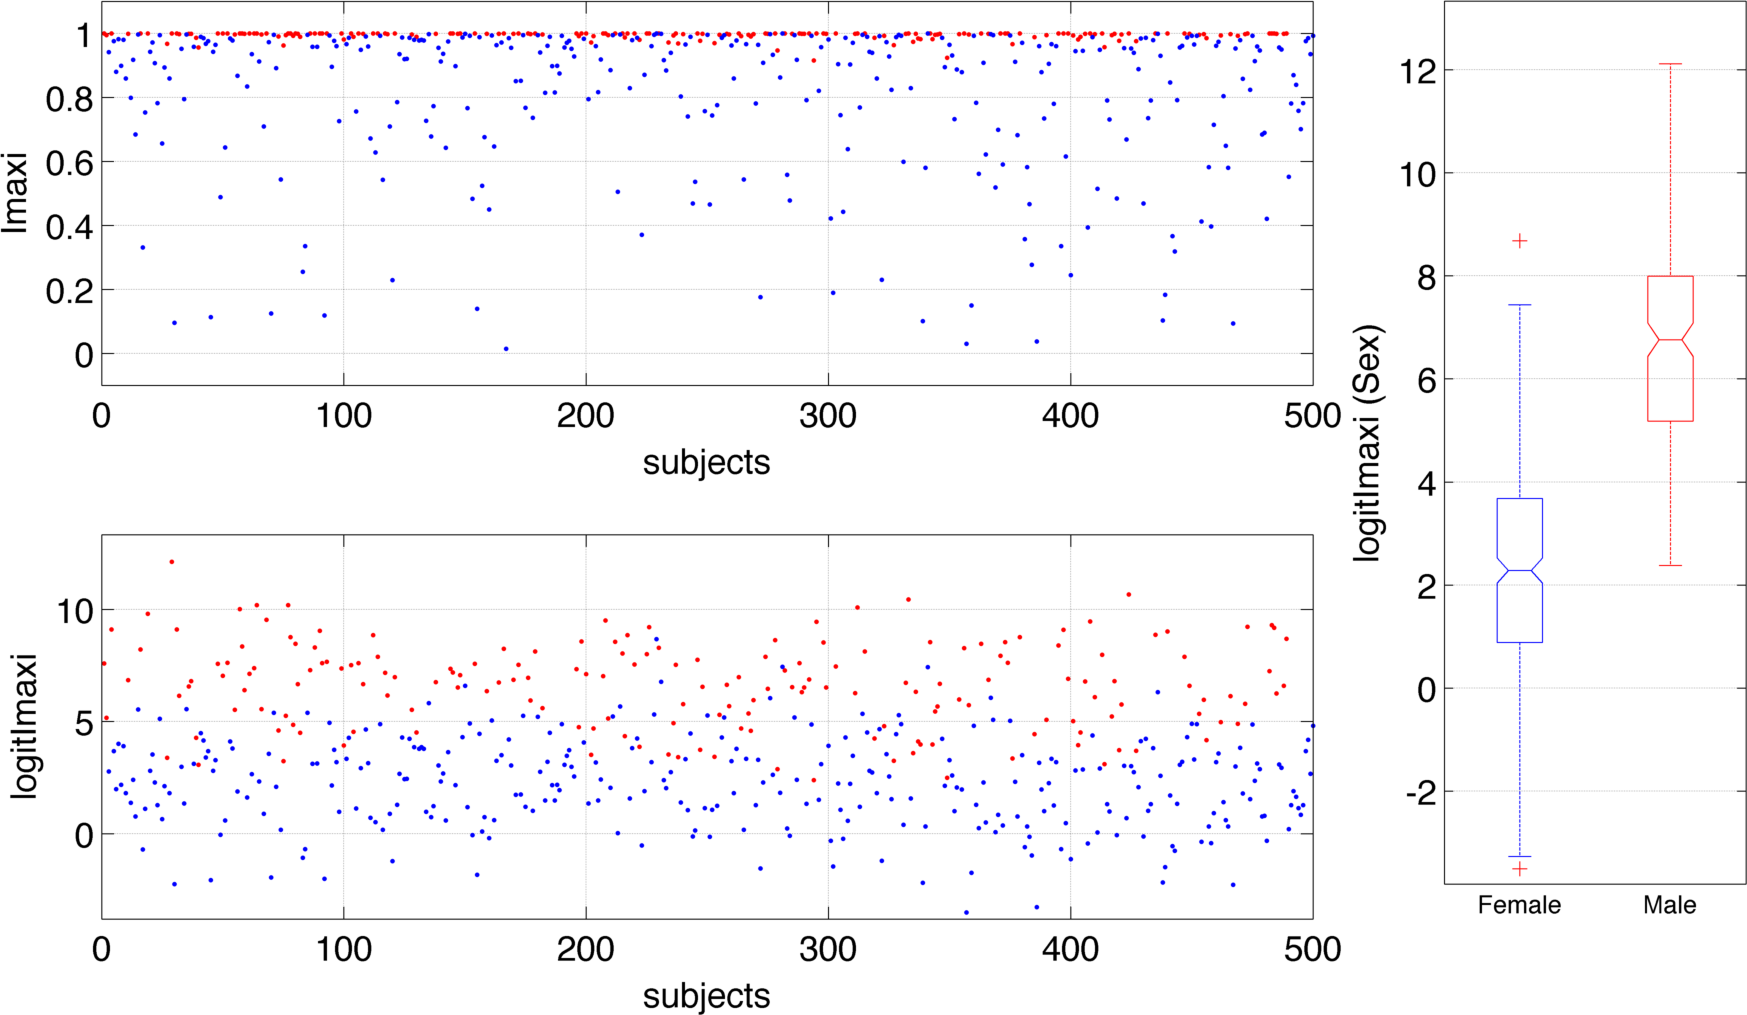
\includegraphics[width=100mm]{paramCovModel_ImaxlogImax_Sex}
%\caption{Logit-normally distributed 'Imax' with 'Sex' as a categorical covariate.}
%\label{fig:parameterCovModel4}
%\end{figure}


%%%%%%%%%%%%%%%%%%%%%%%%%%%%%%%%%%%%%%%%%%%%%%%%%%%%%%%%%%%%%%%%%
% Log-Normal distributed with complex variability structure
%%%%%%%%%%%%%%%%%%%%%%%%%%%%%%%%%%%%%%%%%%%%%%%%%%%%%%%%%%%%%%%%%

\subsubsection{Log-Normal distributed with complex variability structure}
\label{subsec:logIOVCovariate}
In this example we consider representations of type (1) and (2) only. A typical parameter model with a continuous covariate, $W$, for three levels of variability e.g. \{centre, subject, occasion\} (this will be explained in detail in next section), see Figure \ref{tree_IOV1}, reads as follows
\begin{align*}
&(1)\quad V_{lik} = V_{pop} \; \big(\frac{W_i}{70}\big)^\beta \; e^{\eta_{l,V}^{(1)}} \; e^{\eta_{li,V}^{(0)}} \; e^{\eta_{lik,V}^{(-1)}}   \\
&(2)\quad \log(V_{lik}) = \log(V_{pop}) + \beta\log\Big(\frac{W_i}{70}\Big) + \eta_{l,V}^{(1)} + \eta_{li,V}^{(0)} + \eta_{lik,V}^{(-1)}
\end{align*}
with
\begin{align*}
 & \eta_l^{(1)} \sim \mathcal{N}\big(0,\Omega^{(1)}\big), \quad \eta_{li}^{(0)} \sim \mathcal{N}\big(0,\Omega^{(0)}\big),
\quad \eta_{lik}^{(-1)} \sim \mathcal{N}\big(0,\Omega^{(-1)}\big)
\end{align*}
with $l$ -- centre index, $i$ -- subject index, $k$ -- occasion index.


%%%%%%%%%%%%%%%%%%%%%%%%%%%%%%%%%%%%%%%%%%%%%%%%%%%%%%%%%%%%%%%%%
% Discussion
%%%%%%%%%%%%%%%%%%%%%%%%%%%%%%%%%%%%%%%%%%%%%%%%%%%%%%%%%%%%%%%%%
%
%\subsection{Discussion}
%Currently, \pharmml supports the version (2) of the parameter model. Consider the parameter model from last example
%which with some additional annotation reads as follows
%\begin{align*}
%& \underbrace{\log(V_{lik})}_{\text{\parbox{2cm}{\centering transformed\\[-4pt] individual value}}} = \underbrace{\log(V_{pop})}_{\text{\parbox{2cm}{\centering transformed\\[-4pt] typical value}}} + \underbrace{\beta\log\Big(\frac{W_i}{70}\Big)}_{\text{covariate model}}
%+ \underbrace{\eta_{l,V}^{(1)}}_{\text{\parbox{2cm}{\centering inter-centre\\[-4pt]  variability}}}
%+ \underbrace{\eta_{li,V}^{(0)}}_{\text{\parbox{2cm}{\centering inter-individual\\[-4pt] within centre \\[-4pt]  variability}}}
%+ \underbrace{\eta_{lik,V}^{(-1)}}_{\text{\parbox{2.5cm}{\centering inter-occasion\\[-4pt] within individual \\[-4pt] within centre \\[-4pt] variability}}}
%\end{align*}
%This formula, linear for the transformed parameter, has the following \textbf{advantages}
%\begin{itemize}
%\item
%it has an additive structure allowing for easy interpretation and implementation of its components, i.e.
%\begin{itemize}
%\item
%typical/population value of the parameter
%\item
%covariate model
%\item
%any level of random effects
%\end{itemize}
%\item
%it covers the majority of models relevant for daily practice
%\end{itemize}
%The \textbf{disadvantage} is that it doesn't cover parameter models which cannot be represented in the linear form for the transformed parameter, e.g. the models proposed by \cite{Keizer:2011aa}. This issue has been recognised early on and discussed in the consortium. This class of models is being considered for a subsequent specification of \pharmml.


%
%\paragraph{Discussion}
%Consider for example equation (2) for a parameter with a continuous covariate, $W$, with three levels of variability e.g. \{country,subject, occasion\} from the last example. With some additional annotation it reads then
%\begin{align*}
%& \underbrace{\log(V_{lik})}_{\parbox{2cm}{\centering transformed\\[-4pt] individual\\[-4pt] value}} = \underbrace{\log(V_{pop})}_{\parbox{1.5cm}{\centering transformed\\[-4pt] typical\\[-4pt] value}}
%+ \underbrace{\beta\log\Big(\frac{W_i}{70}\Big)}_{\parbox{2cm}{\centering covariate\\[-4pt] model}}
%+ \underbrace{\eta_{l,V}^{(1)}}_{\parbox{2cm}{\centering inter-centre\\[-4pt]  variability}}
%+ \underbrace{\eta_{li,V}^{(0)}}_{\parbox{2.25cm}{\centering inter-centre-\\[-4pt] individual\\[-4pt]  variability}}
%+ \underbrace{\eta_{lik,V}^{(-1)}}_{\parbox{3cm}{\centering inter-centre-\\[-4pt] individual-occasion\\[-4pt] variability}}
%\end{align*}
%
%This formulation, linear for the transformed parameter, has the following advantages
%\begin{itemize}
%\item
%it has an additive structure allowing for easy interpretation and implementation of its components, i.e.
%\begin{itemize}
%\item
%typical/population value of the parameter
%\item
%covariate model
%\item
%inter-individual variability random effects
%\item
%higher levels of variability
%\end{itemize}
%\item
%it covers the majority of models relevant for daily practice
%\end{itemize}
%More complex models will be supported in an upcoming specification.
%


\section{Observation model}
\label{sec:observationModel}
Figure \ref{fig:observModel} gives an overview of the Observation Model as implemented in the current version of PharmML, which covers only continuous data models. A future release will cover discrete data models, such as categorical, count and time-to-event (greyed out in the figure).
\begin{figure}[h!]
\centering
 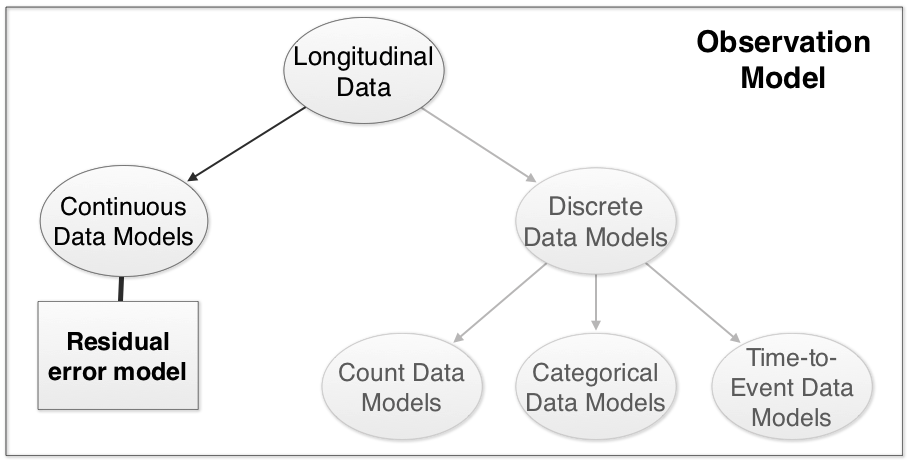
\includegraphics[height=75mm]{observationalModel}
\caption{Observation Model}
\label{fig:observModel}
\end{figure}
An essential component of the Observation Model is the Residual Error Model, which applies only to continuous data models.

%%%%%%%%%%%%%%%%%%%%%%%%%%%%%%%%%%%%%%%%%%%%%%%%%%%%%%%%%%%%%%%%%%
\subsection{Residual error model}
\label{sec:residualErrorModel}
\label{maths:error_model}
\label{maths:combined-err-model}
In this section we consider different forms of the residual error, i.e. this section is about $g$ in the term
\begin{align*}
g(x_{ij}, \psi_{i}, \xi) \epsilon_{ij}
\end{align*}
of eq.\ref{eq:nlmeModel} with $\epsilon_{ij} \sim N(0, 1)$, i.e. a standard normally distributed random variable. We distinguish between
\begin{itemize}\addtolength{\itemsep}{-.95\baselineskip}
\item
models for \textbf{untransformed} data
\begin{align*}
 \underbrace{ y_{ij}}_{\text{\parbox{2cm}{\centering Experimental \\[-4pt]  data}}} =
 \underbrace{ f(x_{ij}, \psi_{i})}_{\text{\parbox{2.5cm}{\centering Model \\[-4pt]  prediction}}} +
 \underbrace{ g(x_{ij}, \psi_{i}, \xi_i) \; \epsilon_{ij}}_{\text{\parbox{3cm}{\centering Residual \\[-4pt] error}}}
 \end{align*}
 \item
\textbf{transform-both-sides} models
\begin{eqnarray}
 \underbrace{ u(y_{ij})}_{\text{\parbox{2cm}{\centering Transformed \\[-4pt] experimental \\[-4pt]  data}}} =
 \underbrace{ u\big(f(x_{ij}, \psi_{i})\big)}_{\text{\parbox{2.5cm}{\centering Transformed \\[-4pt]  model \\[-4pt]  prediction}}} +
 \underbrace{ g(x_{ij}, \psi_{i}, \xi_i) \; \epsilon_{ij}}_{\text{\parbox{3cm}{\centering Residual \\[-4pt] error}}} \nonumber
 \end{eqnarray}
 \item
and \textbf{implicit} models
\begin{eqnarray}
 \underbrace{ u(y_{ij})}_{\text{\parbox{2.5cm}{\centering Transformed \\[-4pt] experimental  data}}} =
 \underbrace{ U\big(f(x_{ij}, \psi_{i}),\xi_i, \epsilon_{1,ij}, \epsilon_{2,ij}, \dots\big)}_{\text{\parbox{2.5cm}{\centering Transformed \\[-4pt]  model prediction}}}
 \end{eqnarray}
\end{itemize}
The \textit{untransformed} form is a special case of the \textit{transform-both-sides} form with $u \equiv Id$, i.e. the identity transformation.
Then for models of both types with $\epsilon_{ij}$ being normally distributed with mean 0 and variance 1, $u(y_{ij})$ is also normally distributed
with mean $u(f(x_{ij}, \psi_{i}))$ and the standard deviation $g(x_{ij}, \psi_{i}, \xi_i)$. \\
Possible extensions to the basic models are
\begin{itemize}
\item
when more than one random variable is applied, i.e. multiple $\epsilon$'s,
\item
when more than one type of measurement or observation is defined, or
\item
when variability, as discussed in section \ref{sec:variabilityModel}, is applied to parameters of the residual error model (see section \ref{subsec:varModelResidualError} for details).
\end{itemize}


%%%%%%%%%%%%%%%%%%%%%%%%%%%%%%%%%%%%%%%%%%%%%%%%%%%%%%%%%%%%%%%%%%
\subsection{Incorporating variability on the residual error model parameters}
\label{subsec:varModelResidualError}
In analogy to the nested hierarchical structure for the variability on the individual parameters,
variability on residual error model parameters can be defined using the same structure.
By doing so, no new structure is necessary to account for any inter-individual and/or inter-occasion variability of the residual error model parameters.

This allows \pharmml to cover the so-called 'ETA-on-EPS' approach -- e.g. IIV on the residual error model parameters or in other words varying residual
error magnitude between individuals, see Figure \ref{fig:IOV0_residualError}.
\begin{figure}[htb!]
\centering
  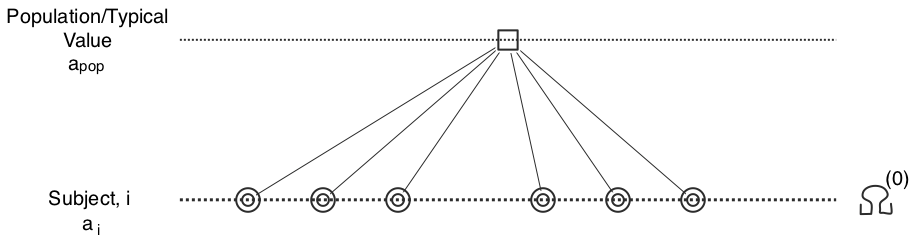
\includegraphics[width=125mm]{pics/IOV0_residualError}
 \caption{Inter-individual variability of the residual error parameter $a$. The nested hierarchical structure is identical to that of structural model parameters.}
 \label{fig:IOV0_residualError}
\end{figure}
For example, if an additive residual error model and a log-normal distribution for $a$ is assumed, then the parameter model reads
\begin{align*}
	& \log(a_i) = \log(a_{pop}) + \eta_a, \quad  \eta_a \sim \mathcal{N}(0,\omega_a^2)
\end{align*}
and the observation model reads
\begin{align*}
	& y_{ij} \sim \mathcal{N}(f_{ij},a_i^2): \quad y_{ij} = f_{ij} + a_i \epsilon_{ij}, \quad \epsilon_{ij} \sim \mathcal{N}(0,1).
\end{align*}
%See also section \ref{modelKK_RM1} for three IIV and IOV examples with NMTRAN and MLXTRAN code.


%%%%%%%%%%%%%%%%%%%%%%%%%%%%%%%%%%%%%%%%%%%%%%%%%%%%%%%%%%%%%%%%%%
\subsection{Residual error model examples}
\label{subsec:modelExamples}
Currently, there is no library of residual error models but this might change in the future. All of the following residual error model examples and their different versions can be implemented in the present version of PharmML:
\begin{itemize}
\item
Constant/additive:
\begin{align*}
& y_{ij} = f_{ij} + a \; \epsilon_{ij}; \quad \epsilon_{ij} \sim N(0,1)  \\
\text{or} \quad & y_{ij} = f_{ij} + \epsilon_{ij}; \quad \epsilon_{ij} \sim N(0,\sigma^2)
\end{align*}
\item
Proportional or constant CV (CCV):
\begin{align*}
&y_{ij} =  f_{ij} + bf_{ij} \; \epsilon_{ij}; \quad \epsilon_{ij} \sim N(0,1)  \\
\text{or} \quad & y_{ij} =  f_{ij}(1+\epsilon_{ij}); \quad \epsilon_{ij} \sim N(0,\sigma^2)
\end{align*}
\item
Combined additive and proportional 1:
\begin{align*}
& y_{ij} =  f_{ij} + (a + bf_{ij}) \; \epsilon_{ij}; \quad \epsilon_{ij} \sim N(0,1)
\end{align*}
\item
Combined additive and proportional 2:
\begin{align*}
& y_{ij} =  f_{ij} + \sqrt{a^2 + b^2f_{ij}^2} \; \epsilon_{ij}; \quad \epsilon_{ij} \sim N(0,1)  \\
\text{or}  \quad & y_{ij} =  f_{ij} +  a\, \epsilon_{1,ij} + b f_{ij}\, \epsilon_{2,ij}; \quad \epsilon_{1,ij} \sim N(0,1); \quad \epsilon_{2,ij} \sim N(0,1);   \\
\text{or}  \quad & y_{ij} =  f_{ij} (1 + \epsilon_{1,ij}) + \epsilon_{2,ij}; \quad \epsilon_{1,ij} \sim N(0,\sigma_1^2); \quad \epsilon_{2,ij} \sim N(0,\sigma_2^2);
\end{align*}
\item
Power error model:
\begin{align*}
& y_{ij} = f_{ij} + b\,f_{ij}^c \; \epsilon_{ij}; \quad \epsilon_{ij} \sim N(0,1)
\end{align*}
\item
Combined additive and power error model 1:
\begin{align*}
& y_{ij} =  f_{ij} + (a + b f_{ij}^c) \; \epsilon_{ij}; \quad \epsilon_{ij} \sim N(0,1)
\end{align*}
\item
Combined additive and power error model 2:
\begin{align*}
& y_{ij} = f_{ij} + a\epsilon_{1,ij} + b f_{ij}^c \epsilon_{2,ij}; \quad \epsilon_{1,ij} \sim N(0,1); \quad \epsilon_{2,ij} \sim N(0,1)
\end{align*}
\item
Two (or more) types of measurements error model:
\begin{align*}
& y_{ij} = f_{ij} + \text{ASY}_j\epsilon_{1,ij} + (1-\text{ASY}_j) \epsilon_{2,ij}; \quad \epsilon_{1,ij} \sim N(0,\sigma_1^2); \quad \epsilon_{2,ij} \sim N(0,\sigma_2^2)
\end{align*}
\item
Two (or more) types of observations error model:
\begin{align*}
& y_{ij} = \text{TYP}_{ij} f_{1,ij} + (1-\text{TYP}_{ij}) f_{2,ij} + \text{TYP}_{ij}\epsilon_{1,ij} + (1-\text{TYP}_{ij}) \epsilon_{2,ij};  \\
&  \epsilon_{1,ij} \sim N(0,\sigma_1^2); \quad \epsilon_{2,ij} \sim N(0,\sigma_2^2)
\end{align*}
%\item
%Extended error model:
%
%y_{ij} = \left\{ \begin{array}{rcl}  f_{ij} + \epsilon_{1,ij}  & \mbox{for} & \text{TIME == 1 \&\& ID == 1} \\
%f_{ij} + \epsilon_{2,ij}  & \mbox{for} & \text{TIME == 2 \&\& ID == 1} \\
%\cdots \end{array}\right\} \quad \text{with} \quad
%\epsilon_{1,ij} \sim N(0,\sigma_1^2),\, \epsilon_{2,ij} \sim N(0,\sigma_2^2), \cdots
%
\end{itemize}
Main sources: \cite{NONMEM:2006aa} and \cite{POPIX:2013}.

\subparagraph{Note 1}
In the list above models are pulled together which have the same variance function.
\subparagraph{Note 2}
Models listed above are the most popular ones in use but the present PharmML structure allows for implementation of virtually any user-defined model. See section ref:XYZ for more examples and PharmML implementation.

%
%%%%%%%%%%%%%%%%%%%%%%%%%%%%%%%%%%%%%%%%%%%%%%%%%%%%%%%%%%%%%%%%%%%
%\subsection{PharmML implementation}
%Some of the above listed residual error model types have two or three equivalent forms, by which we mean they have the same variance, although they use one or more residual errors, $\epsilon_{ij}$. Other types contain two or more predictions from the structural model, \var{f_{ij}}. From a
%computational point of view it makes a lot of sense to reflect such differences in the language structure.
%This was the motivation to allow for the implementation of two types of observation models
%\begin{itemize}
%\item
%\xelem{Standard} -- any observation model of the form
%\begin{align*}
%	u(y_{ij}) = u(f_{ij}) + g\times\epsilon_{ij}
%\end{align*}
%which can be defined using exactly one of the following items
%\begin{itemize}
%\item
%a transformation, $u$, e.g. \var{log} or \var{logit}
%\item
%one structural model prediction, \var{f_{ij}}
%\item
%one standard deviation function, \var{g}
%\item
%one random variable, $\epsilon_{ij}$
%\end{itemize}
%\item
%\xelem{General} -- using any number of the items listed above and arbitrary functional relationship between them.
%\end{itemize}
%Chapter \ref{chap:worked-egs} contains a number of examples illustrating these constructs.

%\begin{itemize}
%\item
%standard -- defined in the spec as \xelem{Standard} with following child elements
%\begin{itemize}
%\item
%\item
%\item
%\end{itemize}
%\item
%general -- defined in the spec as \xelem{General}.
%\end{itemize}




%The residual errors are part of the \textit{Observations Model}, see section \ref{sec:eg1-obs-model} for detailed discussion.
%The following table contains some of the models which can be implemented in \pharmml:
%
%\begin{table}[htdp]
%\begin{center}
%\begin{tabular}{l c c}
%Model name & $g$ & $\xi$ \\
%\hline \hline
%Constant error model & $a$ & $a$ \\
%Proportional error model & $bf$ & $b$ \\
%Combined error model & $a + bf$ & $a,b$ \\
%Alternative combined error model 1& $\sqrt{a^2 + b^2f^2}$ & $a,b$ \\
%Alternative combined error model 2 & $a + bf^c$ & $a, b, c$
%\end{tabular}
%\end{center}
%\caption{Examples of residual error models which can be implemented in \pharmml.}
%\label{tab:residualModels}
%\end{table}%







%\paragraph{Covariate model}
%Covariate model is barely covered so far. See also \cite{Keizer:2011aa}. Missing are following features:\\
%For categorical covariates:\\
%-- categorical distribution of categorical covariates \\
%---- estimating categorical distribution from external data file \\
%---- sampling from known categorical distribution \\
%---- clusters of categorical covariates \\
%For continuous covariates:\\
%-- power-normal distribution for continuous covariates \\
%---- estimating parameters $\lambda$,$\mu$,$\sigma$ from external data file \\
%---- sampling from known power-normal distribution \\
%---- conditional distribution of continuous covariates \\
%------ none \\
%------ defined \\
%------ to be estimated \\
%---- selecting criteria for continuous covariates \\
%---- dependent distribution of continuous covariates \\
%---- correlated continuous covariates \\
%For both types: \\
%-- selection/exclusion criteria missing \\
%
%\subsection{Observation model}
%- Name\\
%- Units\\
%- Observation types - continuous/discrete\\
%- Symbol of predicted output\\
%
%\subsection{Task model}
%-- Combination of tasks, e.g.\\
%1. estimate distribution of covariate from experimental data\\
%2. Simulation task using the estimated PDF
%
%
%\subsection{Not covered so far}
%- correlation of residual errors \\
%---- number models of relevant models identified and described in Use Case document\\
%


%%%%%%%%%%%%%%%%%%%%%%%%%%%%%%%%%%%%%%%%%%%%%%%%%%%%%%%%%%%%%%%%%
%%%%%%%%%%%%%%%%%%%%%%%%%%%%%%%%%%%%%%%%%%%%%%%%%%%%%%%%%%%%%%%%%
\chapter{Trial design model}
\label{sec:CTS}
\label{maths:epoch-defn}

%%%%%%%%%%%%%%%%%%%%%%%%%%%%%%%%%%%%%%%%%%%%%%%%%%%%%%%%%%%%%%%%%
\section{Introduction}

In tools such as NONMEM and MONOLIX it has been common practice to encode the trial design in a data file.
More specifically parts of the overall problem, e.g. the structural model and the parameters are explicitly
encoded in the model file, while other, design related, parts are encoded in the data file. This implies
that the software tool, when processing the data file, must associate the data items with model variables
in order to recognise all characteristics of a study, such as subject-specific measurement time points
and values, covariates, variability levels, etc. This has clear disadvantages for simulation purposes,
because it means that when wanting to change only the design, the data file has to be changed, an error
prone and time consuming work. This is clearly not an ideal situation and PharmML addresses this issue.

It is important to stress that we have based a major part of the trial design on one of the standards 
developed by CDISC "a global, open, multidisciplinary, non-profit organisation that has established 
standards to support the acquisition, exchange, submission and archive of clinical research data 
and metadata" \cite{CDICS:2013}. Over the recent years, this organisation has worked out a set of 
standards widely used in the medical and pharmaceutical research, both in academic and commercial centres. 
Using this standard gives us the reassurance that \pharmml will be able
to represent all trial structures that we are likely to encounter. 


\subsection{Sources of clinical data}

Clinical trials are carefully structured and can vary considerably in
their complexity. Typically, a trial will have one or more arms with
each arm containing one or more treatment regimens and observation
protocols. Individuals are then allocated to each arm from a population
of subjects who have been screened for their suitability to participate
in the trial. In \pharmml we describe the structure and population of a
trial explicitly in a dedicated section. This differs from some other
approaches, but we feel it makes the clinical trial much clearer to
document and easier to encode computationally.


%Typically, in tools such as NONMEM and MONOLIX, the trial design is
%encoded within a tabular data-file. This file contains dosing
%information, covariates and experimental observations for each
%individual in the trial. In addition the definition of the structure
%of the clinical trial is also embedded into this table, meaning that
%the data-file contains a lot of redundant information.

The clinical data comes usually from different sources (and formats) and 
in \pharmml we distinguish this information by separating it into the following three
classes of data dependent on their origin\footnote{It is interesting to note that the developers of
PharML had a similar insight and organised data in a similar
way \cite{NLMEcons:2008}.}:
%
\begin{description}
\item[Population] The attributes of the individuals in the study: the
  population in the population model. Each individual has a weight,
  an age, a gender and numerous other properties that may or may not
  be modelled as covariates in a given model. Importantly, the 'arm' 
  membership of every subject/patient is part of this information.
  In addition, these properties may change over time. 
\item[Dosing] When and how a drug or drugs are administered to the
  individuals in the trial.
\item[Measurements] These are the observations taken from each
  individual at specific times during the study. Such measurements
  provide the objective data used during parameter estimation and are
  typically the outputs calculated during a simulation.
\end{description}

%%%%%%%%%%%%%%%%%%%%%%%%%%%%%%%%%%%%%%%%%%%%%%%%%%%%%%%%%%%%%%%%%
\section{Trial Design}

By separating out these classes of information you can see that the
information we need to define for a clinical trial is as follows:
%
\begin{description}
\item[Structure] The organisation of the trial, how the subjects
  are grouped into different treatment groups and what the dosing
  regimen is within these treatment groups.
\item[Population] As above, the properties specific to the individuals,
  including those that vary over time.
\item[Individual Dosing] This is related to the treatment regimens
  described in the trial structure, but describes the dosing history
  for each individual in the study.
\end{description}
%
The measurement data is then used exclusively for estimation and
is encoded in the third major building block of \pharmml, in the 'Modelling 
Steps'.

%%%%%%%%%%%%%%%%%%%%%%%%%%%%%%%%%%%%%%%%%%%%%%%%%%%%%%%%%%%%%%%%%
\subsection{Structure}
\label{subsec:TrialStructure}

To define the Trial Structure we have reused, almost verbatim, the
CDISC Study Design Model \cite{CDISC:2011a}, which is an
XML representation of a clinical trial. Figure \ref{fig:CellSegmentEpochArmEvent_concept}
below shows how the CDISC trial structure is organised. It has six main components:
\begin{description}
\item[Epoch] The epoch defines a period of time during the study which
  has a purpose within the study. For example a washout or a treatment
  window. In CDISC Epochs can describe screening or follow-up periods,
  which are out of the scope of \pharmml. An epoch is usually defined
  by a time period.
\item[Arm] The arm represents a path through the study taken by a
  subject. An arm is composed of a study cell for each epoch in the study.
\item[Cell] The study cell describes what is carried out during an
  epoch in a particular arm. There is only one cell per epoch.
\item[Segment] The segment describes a set of planned observations and
  interventions, which may or may not involve treatment. Note that in
  \pharmml our definition is more limited and we only describe
  treatments. A segment can contain one or more activities.
\item[Activity] The activity is an action that is taken in the
  study. Here it is typically a treatment regimen or a washout.
\item[StudyEvent] A study event describes the collection of
  information about a particular individual. In CDISC this can be
  information captured during screening or other non-treatment phases
  of the clinical trial. But here we restrict it to capturing
  observations during the treatment. In \pharmml this is how we
  capture occasions.
\end{description}
\begin{figure}[htb]
\centering
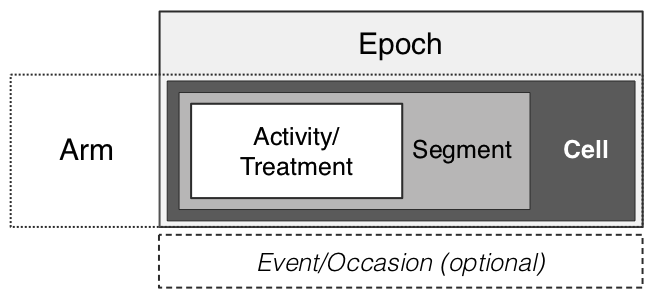
\includegraphics[height=0.2\textheight]{pics/CellSegmentEpochArmEvent_concept}%
\caption{Overview of the basic concept of the Trial Structure: arm,
epoch, event and a cell with segment and activity/treatment as used in the CDISC Study
  Design Model. See the next figure for an example.}
\label{fig:CellSegmentEpochArmEvent_concept}
\end{figure}
\begin{figure}[htb]
\centering
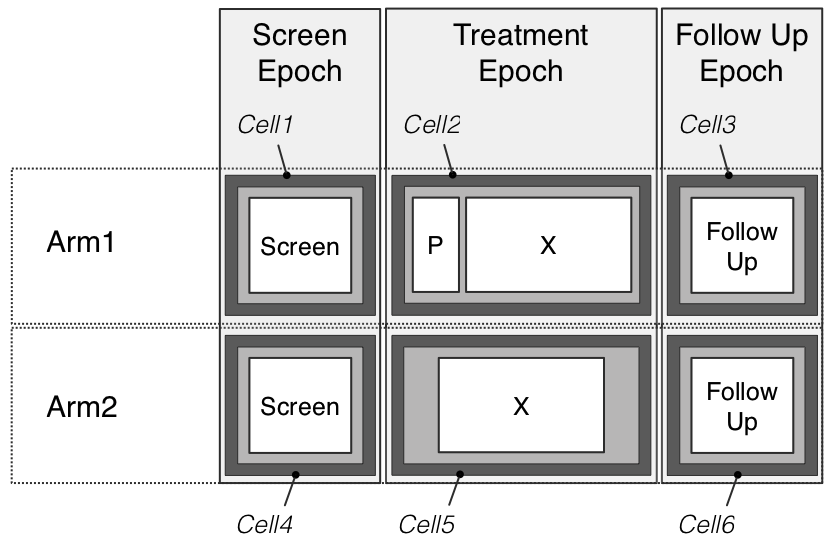
\includegraphics[height=0.35\textheight]{pics/templateTrialDesign}%
\caption{An example of a study with two arms and three epochs: Screen,
Treatment and Follow Up. A segment can contain more then one Activity/Treatment
as can be seen in \var{Cell2} with one Pre-Treatment \var{P} and one Treatment \var{X}.
In this particular example no Event/Occasion is specified.}
\label{fig:templateTrialDesign}
\end{figure}
Figure \ref{fig:templateTrialDesign} shows one such example of a hypothetical trial
consisting of two arms and three epochs: \var{Screen}, \var{Treatment} and
\var{Follow Up}. There are accordingly six cells and segments, each consisting of one
or two activities. \var{Cell2} has the most complex structure carrying two
subsequent treatments, Pre-Treatment \var{P} and Treatment \var{X}. In this case
no Events/Occasions are specified which is an optional element in the design.

Examples of how a trial design is encoded in \pharmml can be found in
the examples (see chapter \ref{chap:worked-egs}).

\paragraph{Variability}
There is one aspect regarding the random variability worth mentioning
here. The \xelem{Population} block carries the information about subject 
level variability and those variability levels above the subject, see next section for more details.  
In the \xelem{Structure} element we encode the variability which is located below the
subject. This is typically known as \textit{inter-occasion variability} but deeper levels
are allowed in theory. The reader is referred to the section \ref{sec:variabilityModel} where the 
full nested hierarchy of the random variability discussed in detail.


%%%%%%%%%%%%%%%%%%%%%%%%%%%%%%%%%%%%%%%%%%%%%%%%%%%%%%%%%%%%%%%%%
\subsection{Population}
\label{subsec:TrialPopulation}

This is the second major element of the trial design description where we:
\begin{itemize}
\item
describe the individuals in the study
\item
describe their attributes (such as weight, gender, etc.)
\item
assign them to an arm of the study, but also
\item
indicate if variability at and/or below the subject level is to be defined, which is the case in the majority of models (if omitted
then this means that we explicitly consider a setup without any random variability,
which is the case for the na\"{\i}ve pooled data method), and
\item
indicate their country or centre membership to define higher levels of variability above the subject level.
\end{itemize}
We define the possible attributes of all individuals using the \var{IndividualTemplate} block and then map
each individual to this template using a \var{Dataset} block.

%\begin{description}
% \item[]
%
% \item[Epoch]
%
% \item[Epoch]
%
%\end{description}

%%%%%%%%%%%%%%%%%%%%%%%%%%%%%%%%%%%%%%%%%%%%%%%%%%%%%%%%%%%%%%%%%
\subsection{Individual dosing}
\label{subsec:TrialSIndivDosing}

The two previous sections on \var{Structure} and \var{Population} described information,
which is sufficient to encode e.g. a simple simulation task. Specifically, when the dosing is 
equal among the patients then this can be encoded in the \var{Structure} part of the schema with
one or more dose amounts and one or more dosing times for all. However, in most cases, especially
when we deal with real clinical data this is not so straighforward. Every patient will have its own specific 
amounts and dosing times.

For an estimation task we always need to provide experimental data for each dosing activity 
relevant to the particular case. With the current structure we can provide individual dosing 
information for every dosing activity defined in the \var{Structure} part (see \ref{subsec:TrialStructure}).

The structure of this part is similar to that used for \var{Population} in that first
a table template is defined with all relevant columns, i.e. \var{ID}, \var{TIME}, and \var{DOSE},
which is then populated with individual dosing data.


%%%%%%%%%%%%%%%%%%%%%%%%%%%%%%%%%%%%%%%%%%%%%%%%%%%%%%%%%%%%%%%%%%
%\subsection{PharmML implementation}
%\label{subsec:TrialSIndivDosingPharmML}
%
%Dependent on the task to be implemented, the information to be stored
%in the Trial Design block will differ. For example an estimation task requires all three
%elements discussed above, which in \pharmml have the intuitive names
%\xelem{Structure}, \xelem{Population} and \xelem{IndividualDosing}
%(see figure \ref{fig:simEstTasks_trialList}). For a simulation task only the first two are
%necessary.
%
%
%\begin{figure}[htb]
%\centering
%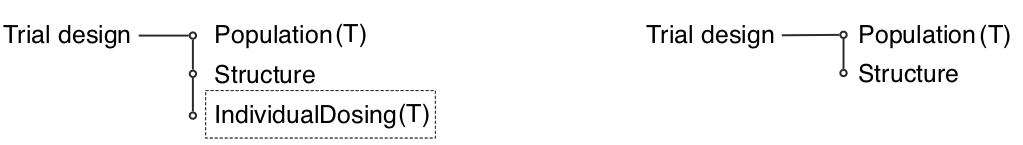
\includegraphics[width=0.7\linewidth]{pics/simEstTasks_trialList}%
%\caption{PharmML building blocks used in the definition of a trial design.}
%\label{fig:simEstTasks_trialList}
%\end{figure}


%%%%%%%%%%%%%%%%%%%%%%%%%%%%%%%%%%%%%%%%%%%%%%%%%%%%%%%%%%%%%
%\begin{figure}[htbp!]
%\centering
%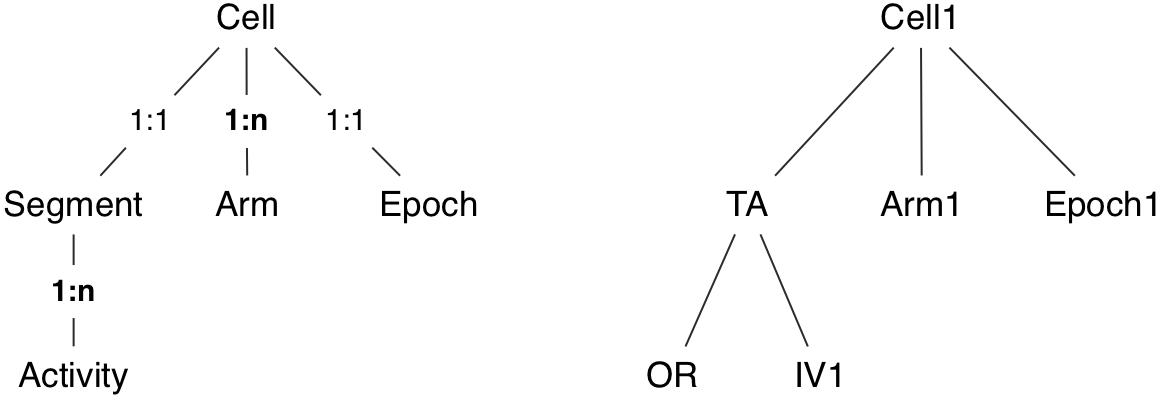
\includegraphics[width=0.8\linewidth]{../pics/cellHierarchy2}
%\caption{General cell hierarchy (left); The root of the hierarchy is the cell which can contain one segment, one epoch and multiple arms. The segment element can have multiple child elements, the activities e.g. treatments or a washout. (right) An example of how it is applied in this example.}
%\label{fig:cellHierarchy}
%\end{figure}

%\section{Design elements and examples}
%\label{sec:CTS_exampleSection} % KEEP THIS LABEL!!!!!!
%The default working mode, as mentioned above, is when all the study characteristics are encoded in the data file. Alternatively, PharmML offers a very flexible structure for the setup of clinical trials. Using only a few basic elements the modeller can compose several types of designs, including parallel design and crossover designs with or without washout or run-in period\footnote{\textit{Run-in} -- do be continued. Definition after \cite{Iverson:2007fk}}, see Figure \ref{fig:CTSfigure1} for examples. The basic elements are:
%
%\begin{itemize}
%\item
%%\textit{Dosing}
%%\begin{itemize}
%%\item
%%one or multiple dosing events can be defined
%%\item
%%dosing type: single dose, sequence/repeated or steady-state dosing
%%\item
%%type of administration: bolus or infusion
%%\item
%%target compartment/variable
%%\item
%%amount and/or infusion rate
%%\item
%%dosing times
%%\end{itemize}
%%\item
%\textit{Treatment} -- describes dosing related data
%\begin{itemize}
%\item
%Administration/dosing type, \textit{Bolus} or \textit{Infusion}, as single value or a sequence
%\item
%Dosing Times -- as single value or a sequence
%\item
%Dose Amount -- as single value or a sequence
%\item
%Dosing target
%\begin{itemize}
%\item
%Target variable (indicates the target compartment) -- for ODE coded structural models, e.g. $Ad$ the drug amount in the depot compartment (see section \ref{sec:structuralModel})
%\item
%Dose variable -- for explicit algebraic equations with a dose amount variable, e.g. $D$ as in $C(t)= \frac{D}{V}e^{-k(t-t_D)}$
%\end{itemize}
%\end{itemize}
%\item
%\textit{Treatment Epoch\footnote{\textit{Epoch} -- Interval of time in the planned conduct of a study. An epoch is associated with a purpose (e.g., screening, randomization, treatment, follow-up), which applies across all arms of a study. NOTE: Epoch is intended as a standardised term to replace: period, cycle, phase, stage. Definition after \cite{CDICS:2011}}} -- basic time interval within a study
%\begin{itemize}
%\item
%Epoch name, e.g. \textit{Treatment\_A} or \textit{Washout}\footnote{\textit{Washout} -- A period in a clinical study during which subjects receive no treatment for the indication under study and the effects of a previous treatment are eliminated (or assumed to be eliminated).} or \textit{Run-in}
%\item
%\textit{Start time} and \textit{end time} of an epoch -- this sets reference time frame for any possible occasion within an epoch
%\item
%Occasion(s) -- defined by
%\begin{itemize}
%\item
%\textit{start time} and \textit{end time} of each occasion relative to epoch time frame
%\item
%level identifier
%\end{itemize}
%\end{itemize}
%\item
%\textit{Group} -- basic grouping structure for subjects usually containing one or more treatment epochs
%\begin{itemize}
%\item
%a sequence of epochs for a number of subjects, e.g. [\textit{Epoch\_A}, \textit{Washout}, \textit{Epoch\_B}]
%\item
%number of subjects
%\end{itemize}
%\end{itemize}
%
%\paragraph{Note 1} The name of a particular trial design, e.g. \textit{parallel} or \textit{crossover with washout} is not part of the language. It can be provided as annotation of the trial design model using an appropriate ontology.
%\paragraph{Note 2} The 'Washout' epoch means complete reset of all variables and is defined without start and end times, but this restrictions will be released in an upcoming specification.
%\paragraph{Note 3} The support for variability levels is limited in this specification of PharmML. More specifically, it can only encode occasions definable using start and end times for each occasion. Levels above the subject reference level, such as 'country' or 'centre' cannot be encoded.
%


%\begin{figure} % [htb!]
%\centering
%\begin{tabular}{c}
% 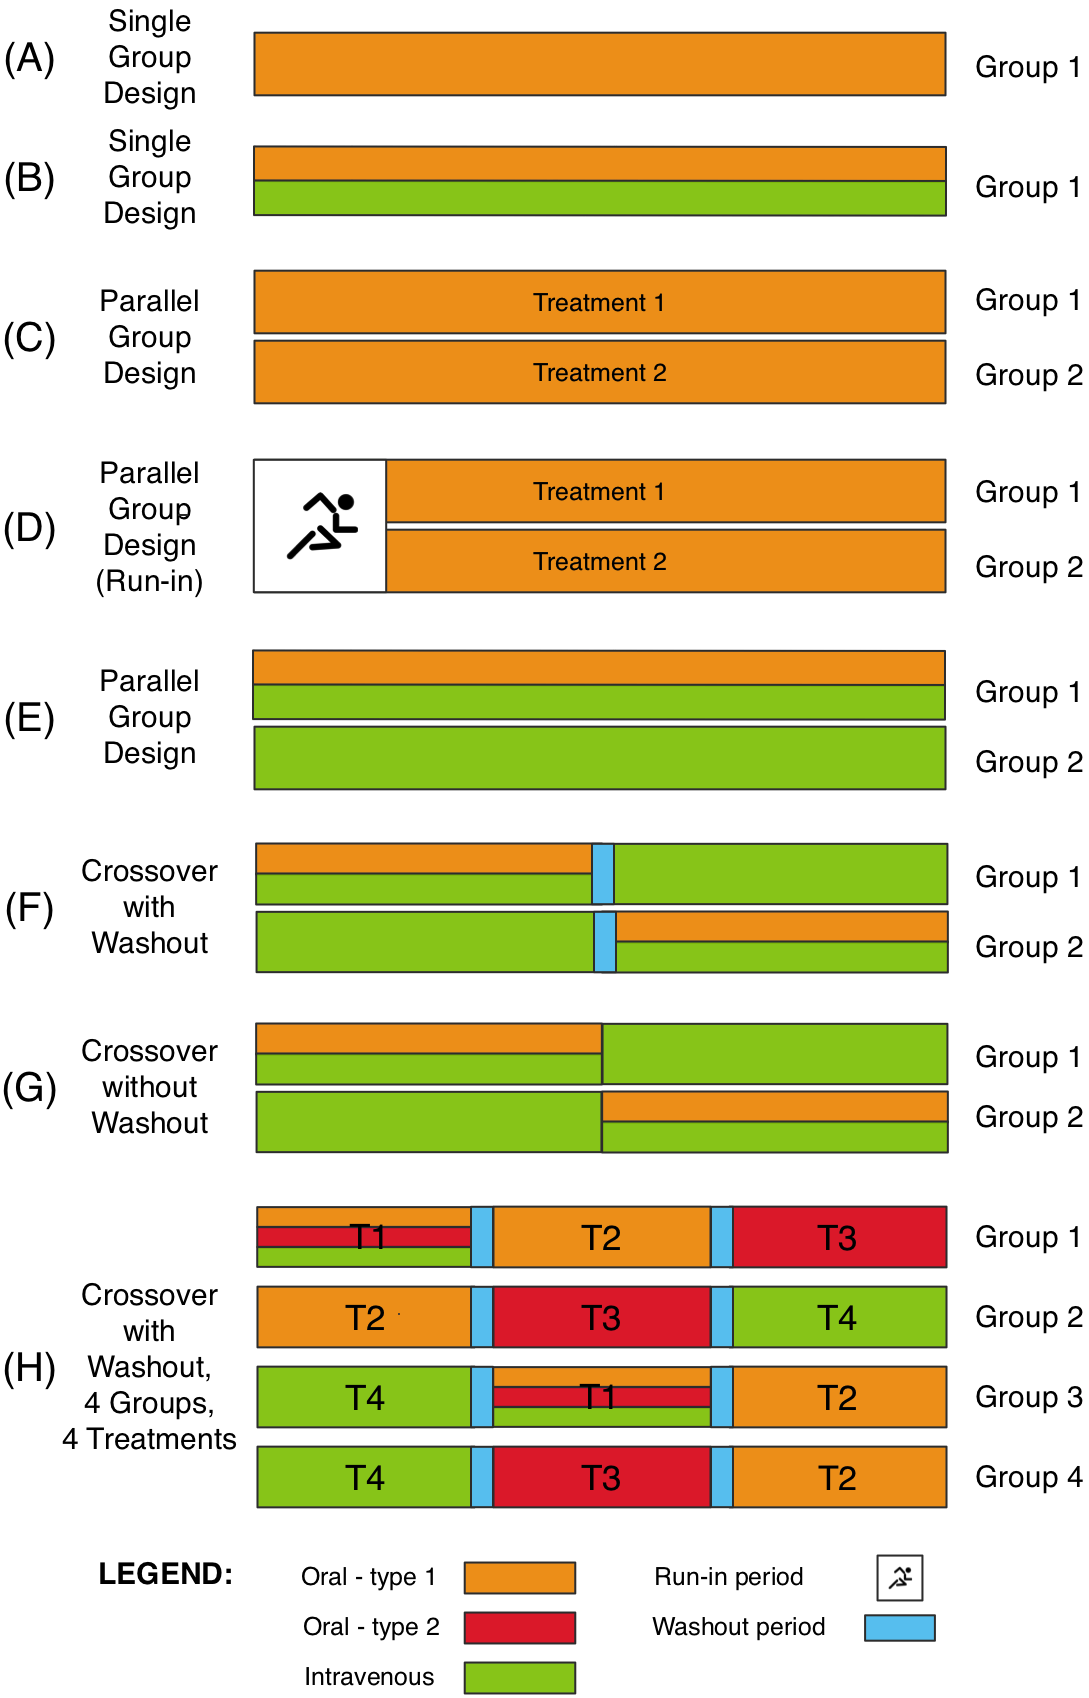
\includegraphics[width=140mm]{ClinicalDesignPatterns_version3}
% \end{tabular}
%\caption{Examples for basic clinical trial design types and configurations. In general any combination of the basic structural elements, i.e. \textit{Dosing}, \textit{Treatment}, \textit{Treatment Epoch} and \textit{Group}, can be created. Based on \cite{Lavielle:2012} and \cite{Wang:2006}.}
%\label{fig:CTSfigure1}
%\end{figure}


%%%%%%%%%%%%%%%%%%%%%%%%%%%%%%%%%%%%%%%%%%%%%%%%%%%%%%%%%%%%%%%%%
%\subsection{Example 1 -- Basic crossover with washout}
%This example describes a crossover design\footnote{\textit{Crossover design} -- Each subject is allocated to a sequence of treatments across a number of treatment periods. Within crossover trials, sequences can include all possible treatments or a subset of these (incomplete block). Definition after \cite{CDICS:2011}} with washout, see example F in Figure \ref{fig:CTSfigure1}.
%
%\subsubsection{Trial design model}
%
%-- Treatment definition
%\begin{align*}
%Treatment\_A: & AdministrationType = \text{[OR bolus, IV bolus]}  \\
%& DoseTime = [6:24:72, 0:24:72]   \\
%& DoseSize = [50, \;\;100]   \\
%& DoseVariable = \text{[D, \;\;D]}  \\
%Treatment\_B: & AdministrationType = \text{OR bolus}  \\
%& DoseTime = 0:24:72   \\
%& DoseSize = 150   \\
%& DoseVariable = \text{D}
%\end{align*}
%
%-- Treatment Epoch definition
%\begin{align*}
%Epoch\_1: & Treatment\_A  \\
%& TreatmentStart = 0  \\
%& TreatmentEnd = 100  \\
%Epoch\_2: & Treatment\_B  \\
%& TreatmentStart = 0  \\
%& TreatmentEnd = 100  \\
%Epoch\_3: & Washout
%\end{align*}
%
%-- Group definition
%\begin{align*}
%Group 1: 	& TreatmentSeq = \text{[Epoch\_1, Epoch\_3, Epoch\_2]}	 \\
%			& GroupSize = 40		 \\
%Group 2: 	& TreatmentSeq = \text{[Epoch\_2, Epoch\_3, Epoch\_1]}  \\
%			& GroupSize = 60
%\end{align*}
%
%
%%%%%%%%%%%%%%%%%%%%%%%%%%%%%%%%%%%%%%%%%%%%%%%%%%%%%%%%%%%%%%%%%
%\subsection{Example 2 -- Complex crossover trial with washout, 4 groups}
%See example H in Figure \ref{fig:CTSfigure1}.
%
%\subsubsection{Trial design model}
%
%-- Treatment definition
%\begin{align*}
%T1: & AdministrationType = \text{[OR1, OR2, IV]}  \\
%& DoseSize = [50 \;\;\;100 \;\;\;100];   \\
%& DoseTime = [6:24:72, 0:24:72, 12:24:72];   \\
%& DoseVariable = \text{[D, \;\;D, \;\;D]}  \\
%T2: & AdministrationType = \text{OR1}  \\
%& DoseSize = 150;   \\
%& DoseTime = [0:24:72];    \\
%& DoseVariable = \text{D}  \\
%T3: & AdministrationType = \text{OR2}  \\
%& DoseSize = 150;   \\
%& DoseTime = [0:24:72];   \\
%& DoseVariable = \text{D}  \\
%T4: & AdministrationType = \text{IV}  \\
%& DoseSize = 150;   \\
%& DoseTime = [0:24:72];   \\
%& DoseVariable = \text{D}
%\end{align*}
%
%
%-- Treatment Epoch definition
%\begin{align*}
%Epoch\_1: & T1  \\
%& TreatmentStart = 0  \\
%& TreatmentEnd = 100  \\
%Epoch\_2: & T2  \\
%& TreatmentStart = 0  \\
%& TreatmentEnd = 100  \\
%Epoch\_3: & T3  \\
%& TreatmentStart = 0  \\
%& TreatmentEnd = 100  \\
%Epoch\_4: & T4  \\
%& TreatmentStart = 0  \\
%& TreatmentEnd = 100  \\
%Epoch\_5: & Washout
%\end{align*}
%
%
%-- Group definition
%\begin{align*}
%Group 1: 	& TreatmentSeq = \text{[Epoch\_1, Epoch\_5, Epoch\_2, Epoch\_5, Epoch\_3]}	 \\
%			& GroupSize = 40		 \\
%Group 2: 	& TreatmentSeq = \text{[Epoch\_2, Epoch\_5, Epoch\_3, Epoch\_5, Epoch\_4]}  \\
%			& GroupSize = 40		 \\
%Group 3: 	& TreatmentSeq = \text{[Epoch\_4, Epoch\_5, Epoch\_1, Epoch\_5, Epoch\_2]}	 \\
%			& GroupSize = 60		 \\
%Group 4: 	& TreatmentSeq = \text{[Epoch\_4, Epoch\_5, Epoch\_3, Epoch\_5, Epoch\_2]}  \\
%			& GroupSize = 60
%\end{align*}





%%%%%%%%%%%%%%%%%%%%%%%%%%%%%%%%%%%%%%%%%%%%%%%%%%%%%%%%%%%%%%%%%
%\subsubsection{To-Do list}
%
%\paragraph{Crossover - other aspects not covered yet}
%- 2x2 -- covered already \\
%- p x q -- see Table 2 in \cite{Wang:2006} \\
%- Latin square 3x3 \& 4x4
%
%
%%%%%%%%%%%%%%%%%%%%%%%%%%%%%%%%%%%%%%%%%%%%%%%%%%%%%%%%%%%%%%%%%
%\paragraph{Factorial design}
%In a factorial design two or more treatments are evaluated simultaneously through the use of varying combinations of the treatments. The simplest example is the 2x2 factorial design in which subjects are randomly allocated to one of the four possible combinations of two treatments, A and B say. These are: A alone; B alone; both A and B; neither A nor B. Source: \cite{EMA:1998}\\
%- no example available
%
%\paragraph{Other aspects of factorial design to be considered}
%- 2x2, Ix J x K, unbalanced, 'complicated'
%
%
%%%%%%%%%%%%%%%%%%%%%%%%%%%%%%%%%%%%%%%%%%%%%%%%%%%%%%%%%%%%%%%%%
%\paragraph{Cohort study}
%Study of a group of individuals, some of whom are exposed to a variable of interest, in which subjects are followed over time. Cohort studies can be prospective or retrospective. [AMA Manual of Style] See also prospective study.
%
%%%%%%%%%%%%%%%%%%%%%%%%%%%%%%%%%%%%%%%%%%%%%%%%%%%%%%%%%%%%%%%%%
%\paragraph{Prospective study}
%Investigation in which a group of subjects is recruited and monitored in accordance with criteria described in a protocol.
%
%
%%%%%%%%%%%%%%%%%%%%%%%%%%%%%%%%%%%%%%%%%%%%%%%%%%%%%%%%%%%%%%%%%
%\paragraph{Survival}
%Observe N subjects until at most time T (censored observations). Alternatively observe N subjects until at least R events occur.\\
%- no example available
%
%
%%%%%%%%%%%%%%%%%%%%%%%%%%%%%%%%%%%%%%%%%%%%%%%%%%%%%%%%%%%%%%%%%
%\paragraph{Observational}
%Subjects are not randomly allocated to treatment.\\
%- no examples available
%
%
%%%%%%%%%%%%%%%%%%%%%%%%%%%%%%%%%%%%%%%%%%%%%%%%%%%%%%%%%%%%%%%%%
%\paragraph{Dose escalation Methods in Phase I, \cite{Le-Tourneau:2009fk}}
%-- Rule-based designs: \\
%Traditional 3+3 design, Accelerated titration designs, Pharmacologically guided dose escalation\\
%Model-based designs: \\
%-- Modified continual reassessment method, Escalation with overdose control, Time-to-event continual reassessment method, EffTox -- efficacy and toxicity method, TriCRM -- an adaptive continual reassessment method that considers three potential trial outcomes: no efficacy and no toxicity, efficacy only, and toxicity only\\
%
%%%%%%%%%%%%%%%%%%%%%%%%%%%%%%%%%%%%%%%%%%%%%%%%%%%%%%%%%%%%%%%%%
%\paragraph{Additional option/criteria -- from Mike's list}
%Within each of these general types of study there are several possible flavours:\\
%Titration, Forced titration, Target concentration, Adaptive, With stopping rules, With interim analyses\\
% - no examples available
%
%%%%%%%%%%%%%%%%%%%%%%%%%%%%%%%%%%%%%%%%%%%%%%%%%%%%%%%%%%%%%%%%%
%\paragraph{Other classification criteria}
%
%\paragraph{Blinding:}
%open/unblinded, single/double/triple  blinded
%
%\paragraph{Order of study}
%- pxq, IxJxK









%\part{Technical Description}

% This section provides and overview of the design of PharmML. The design
% principles etc and an orientation around PharmML for the non-IT professional.

\newcommand{\phsec}[1]{{\slshape #1}}
\chapter{Language Overview}
\label{chap:lang-overview}

\section{Introduction}

In this chapter we will provide you with the background knowledge you
need to understand \pharmml. We recommend that you read this chapter
before you work through the examples in chapter
\ref{chap:worked-egs}. The chapter will start by describing how a
\pharmml document is organised and then go on to illustrate some of
the key concepts and constructs of the language. For example, among
other things, we discuss variable and parameter scoping (section
\ref{sec:scoping-rules}), how to write maths (sections~\ref{sec:odes}
and~\ref{sec:maths}), and how to define data (section~\ref{sec:dataset}).
%and how to define and use units (section~\ref{sec:units}).
The chapter concludes with a discussion of the additional resources that
we expect to be used in support of \pharmml, but which are outside the
scope of this language specification (section~\ref{sec:supporting-res}).

\section{Organisation}
\label{sec:structure-overview}

As can be seen in figure \ref{fig:momloverview}, \pharmml is organised
into three main sections: \phsec{Model Definition}, \phsec{Trial
  Design} and \phsec{Modelling Steps}. This reflects the natural
organisation of a pharmacometric model and is the organisation
implicitly found in the M\&S tools used by modellers in this
area. Below we will go into more detail about the purpose and
organisation of each section.

% The
% \phsec{Model Definition} describes the model to be simulated, for
% which parameters are to be estimated, or which is to be analysed. The
% \phsec{Modelling Steps} section describes the process(es) used to
% simulate the model or estimate its parameters. Finally we have the
% \phsec{Trial Design} section. This describes the design of a clinical
% trial within \pharmml.

\begin{figure}[htb]
 \centering
  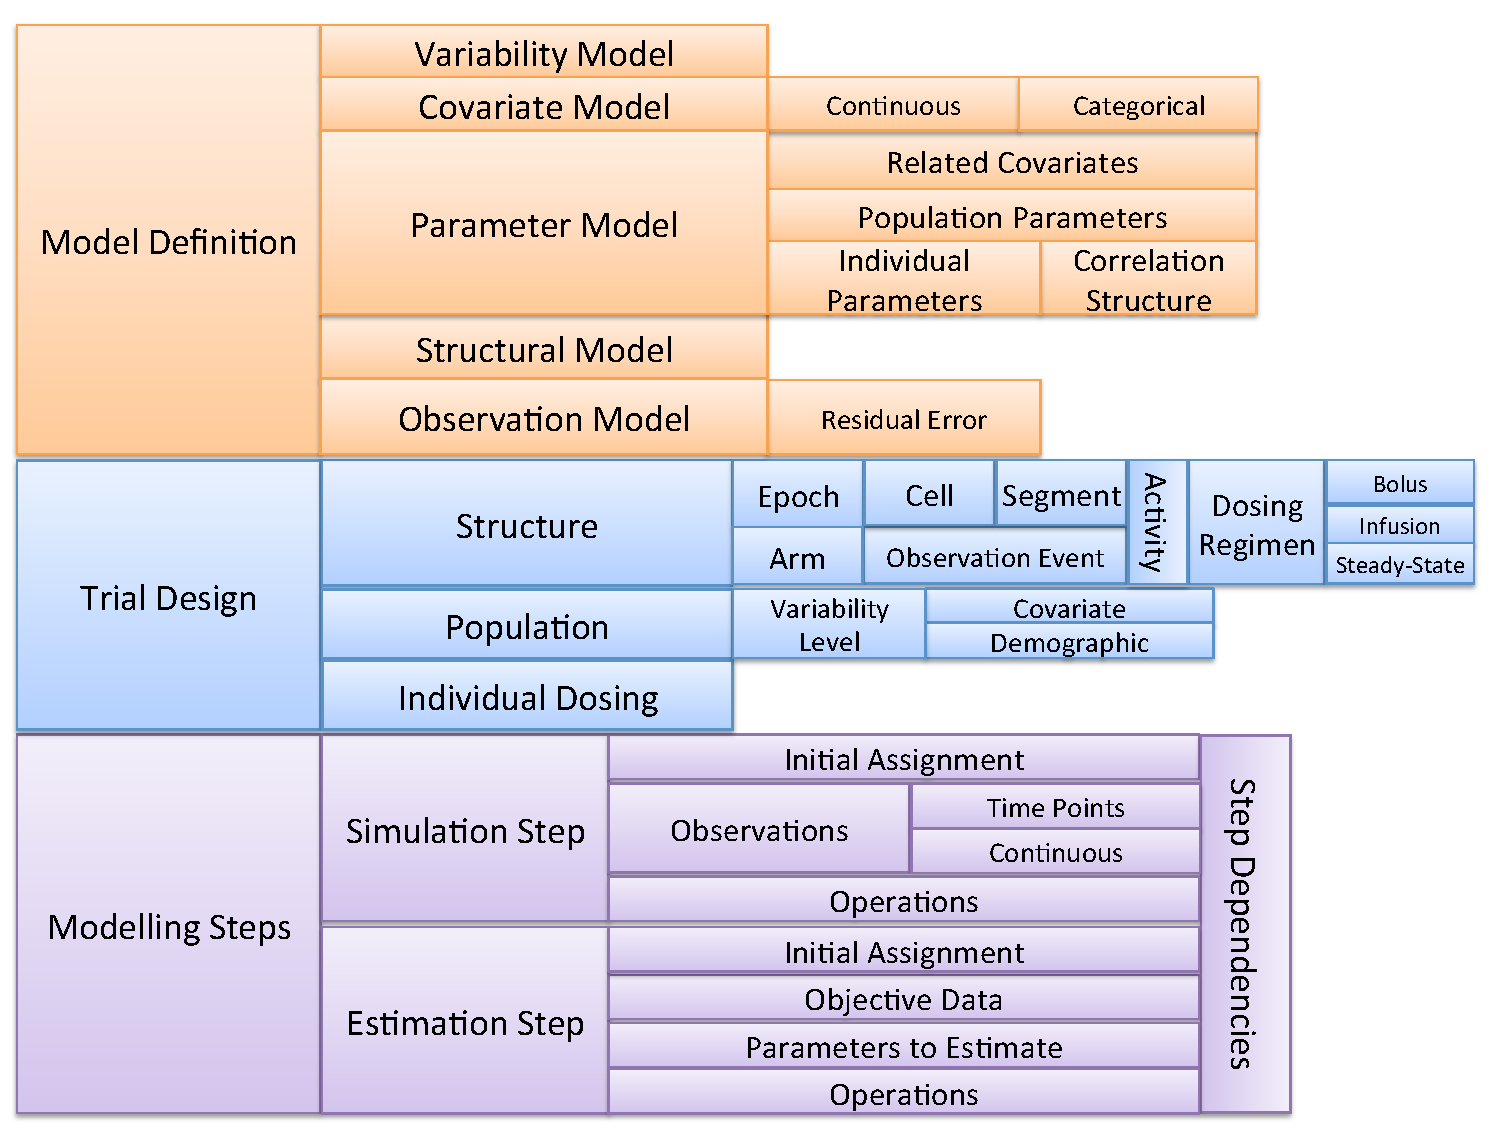
\includegraphics[height=0.4\textheight]{OverviewOfMoML}
  \caption{An overview of the organisation of \pharmml.}
  \label{fig:momloverview}
\end{figure}

% Below we will describe each section in more detail, but at this point it
% is worth noting that the \emph{minimal} \pharmml document describing a
% pharmacometric model must contain a \phsec{Model Definition}. It is
% also possible to describe a valid model with the \phsec{Model Definition} and
% \phsec{Trial Design}; and of course all three sections.

%Typically, this model could be reused in different
%scenarios and it is not necessarily specific to a particular clinical
%trial or simulation.

\subsection{Model Definition}

The \phsec{Model Definition} defines the model, typically a population
model, that describes the system under investigation and any variability
between individuals in the population. The modeller may wish to use
it for simulation, parameter estimation or other types of analysis and
exploration. The \phsec{Model Definition} in turn is composed of another
set of ``models'' that describe specific aspects of the overall model
definition. These are described below.

\subsubsection{Variability Model}
\label{sec:variability_model}

Variability is the concept that underpins a pharmacometric model and
the \phsec{Variability Model} enables us to describe this. Note that it
is possible to describe variability in a \pharmml model without
defining random variability, but by using covariates.
%\footnote{see Marc L.'s email [PUT URL HERE].}
Therefore the use of the \phsec{Variability Model}
is optional. In \pharmml you can use this to define
individual random variability, but also a hierarchy of variability
above and/or below the level of the individual (e.g.\xspace inter-occasion
variability). For more details of the theory behind the random
variability model, see section \ref{sec:variabilityModel}.


\subsubsection{Covariate Model}

The \phsec{Covariate Model} as you would expect from the name describes the
covariates used in the \phsec{Model Definition}. A covariate can be
continuous, in which case it is typically described by a continuous probability
distribution, or categorical. The formal description of the covariate
model can be found in section \ref{maths:covariate_model}.

\subsubsection{Parameter Model}

The \phsec{Parameter Model} principally describes the parameters of the model
definition and is typically used to describe parameters with some
level of variability (typically between subject variability). The
parameter is defined more formally in section
\ref{maths:parameter_defn}, but essentially for each parameter we
define a population term, one or more random effects, and its
relationship to the covariates defined in the covariate model. The
random effects can be defined at different levels of variability
(defined by the variability model, see section
\ref{sec:variability_model}), which includes capturing the correlation
between them --- essentially defining a covariance (or correlation)
matrix for each level of variability.

\subsubsection{Structural Model}

At the heart of the model definition are one or more \phsec{Structural
Model}s. These describe the system or systems that a modeller is
interested in and they represent a particular abstraction of that
system. For example a structural model may be used to describe the
pharmacokinetics of a drug. We can represent PK, PD or PK-PD models as
combinations of ODEs and algebraic equations.

\subsubsection{Observation Model}

In clinical trials experimental observations are made, and these
observations are subject to experimental error. Different types of
instrument, assay or material sampled will all have different
statistical errors associated with them. In a pharmacometric model
these errors are described using a residual error model (see
section~\ref{maths:error_model}). In \pharmml we encode the residual
error model using the \phsec{Observation Model}.

% The language permits the
% encoding of the more structured \emph{standard} and more flexible
% \emph{general} definition (this is described in more detail in
% section~\ref{maths:error_model}).

The outcomes of a clinical trial that we wish to model are not always
experimental measurements. A trial may aim to determine the efficacy
of an analgesic using a pain score provided by the subject; or measure
the frequency of seizure based on the maximum drug concentration; or
establish the remission rate over a given time in a cancer trial
\cite{Bonate:2011fk}. In each of these cases one needs to use a
discrete statistical model to represent these outcomes. These will
also be defined in the Observation Model, but at the moment are not
supported by the current version of \pharmml (see chapter
\ref{chap:scope}).

\subsection{Trial Design}

Clinical trials are carefully structured and can vary considerably in
their complexity. Typically, a trial will be structured into one or
more groups with each group subject to one or more treatment regimens
and observation protocols. Each group is then populated with individuals
from a population of subjects who have been screened for their
suitability to participate in the trial. In \pharmml we describe
the structure and population of a trial
explicitly in a dedicated section. This differs from some other
approaches, bit we feel it makes the clinical trial much clearer to
document and easier to encode computationally. More information can be
found in chapter~\ref{sec:CTS}.

% Typically in tools such as NONMEM and MONOLIX, the trial design is
% encoded within a tabular data-file. This file contains the dosing
% information, covariates and the experimental observations of each
% individual in the trial. In addition the definition of the structure
% of the clinical trial is also embedded in this table too. Clearly the
% data-file contains a lot of redundant information.

% In \pharmml we separate this information into the following three
% classes\footnote{It is interesting to note that the developers of
%   PharML had a similar insight and organised data in a similar
%   way\cite{NLMEcons:2008}.}:
% %
% \begin{description}
% \item[Population] The attributes of the individuals in the study: the
%   population in the population model. Each individual has a weight,
%   an age, a gender and numerous other properties that may or may not
%   be modelled as covariates in a given model. In addition, these
%   properties may change over time.
% \item[Dosing] When and how a drug or drugs are administered to the
%   individuals in the trial.
% \item[Measurements] These are the observations taken from each
%   individual and specific times during the study. Such measurements
%   provide the observations used during parameter estimation and are
%   typically the outputs calculated during a simulation.
% \end{description}
% %
% By separating out these classes of information you can see that the
% information we need to define the clinical trial is as follows:
% %
% \begin{description}
% \item[Trial Structure] The organisation of the trial, how the subjects
%   are grouped into different treatment groups and what the dosing
%   regiment is within these treatment groups.
% \item[Population] As above, the properties specific to the individual,
%   including those that vary over time.
% \item[Individual Dosing] This is related to the treatment regimens
%   described in the trial structure, but describes the dosing of each
%   subject in the study.
% \end{description}
% %
% The measurement data is then used exclusively for estimation.

% \begin{figure}[htb]
% \centering
% 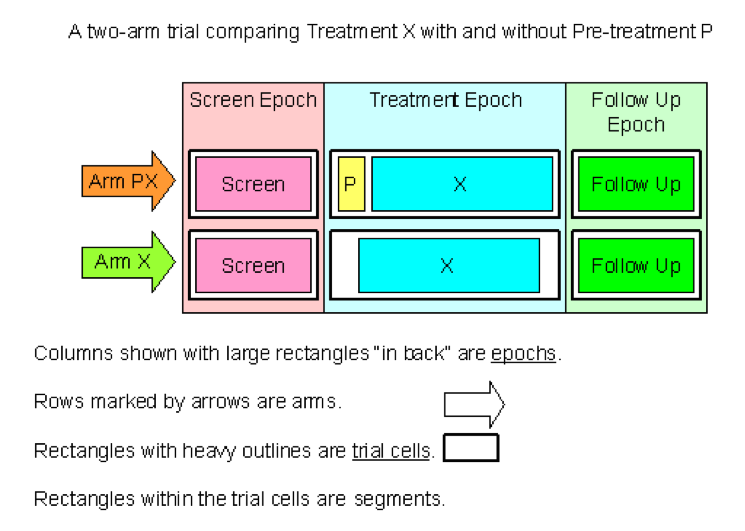
\includegraphics[height=0.35\textheight,clip=true,trim=0 0.5cm 0 0]{change_proposals/CDISCTrialStructure}%
% \caption{Overview of the Trial Structure used in the CDISC Study
%   Design Model.}
% \label{fig:cdiscstruct}
% \end{figure}

%  To define the Trial Structure we have reused, almost verbatim, the
% CDISC Study Design Model\footnote{CDISC URL to go here.}, which is an
% XML representation of a clinical trial. The figure below (figure
% \ref{fig:cdiscstruct}) shows how the CDISC trial structure is
% organised. It has five main components:
% \begin{description}
% \item[Epoch] The epoch defines a period of time during the study which
%   has a purpose within the study. For example a washout or a treatment
%   window. In CDISC Epochs can describe screening or follow-up periods,
%   which are out of the scope of \pharmml. An epoch is usually defined
%   by a time period.
% \item[Arm] The arm represents a path through the study taken by a
%   subject. An arm is composed of a study cell for each epoch in the study.
% \item[Cell] The study cell describes what is carried out during an
%   epoch in a particular arm. There is only one cell per epoch.
% \item[Segment] The segment describes a set of planned observations and
%   interventions, which may or may not involve treatment. Note that in
%   \pharmml our definition is more limited and we only describe
%   treatments. A segment can contains one or more activities.
% \item[Activity] The activity is an action that is taken in the
%   study. Here it is typically a treatment regimen.
% \item[StudyEvent] A study event describes the collection of
%   information about a particular individual. In CDISC this can be
%   information captured during screening or other non-treatment phases
%   of the clinical trial. But here we restrict it to capturing
%   observations during the treatment. In \pharmml this is how we
%   capture occasions.
% \end{description}
%  %
% Using this design gives us the reassurance that \pharmml will be able
% to represent all trial structures that we are likely to encounter.

% Examples of how a trial design is encoded in \pharmml can be found in
% the examples (chapter~\ref{chap:worked-egs}).


\subsection{Modelling Steps}
\label{sec:stepdeps}
The final element when describing an M\&S experiment, after defining
the model and the associated trial design, is to describe how the
model was used. This section of a \pharmml document is akin to the
Methods section of a paper. The aim is not to replicate your modelling
exactly, but to provide enough information to reproduce the
model\footnote{To replicate the execution of a model requires detailed
  information about not only what algorithms were used to simulate or
  execute a model, but also what software implementation was used and
  exact supporting libraries such as that of the random number
  generator.}.

\section{Identifiers, references and namespaces}

In \pharmml we use the Object Identifier to identify components in the
\phsec{Trial Design} and \phsec{Modelling Steps} sections of a \pharmml document and
the Symbol Identifier to identify parameters and variables within the
\phsec{Model Definition} section. Below we will describe the rules associated
with how they are defined and referenced.


\subsection{Object identifiers}

The concept of the Object Identifier is borrowed from the CDISC XML
description of a trial design \cite{CDISC:2011a}. There they use the
attribute \xatt{oid} to identify and to reference components used in
the design. Object identifiers have global scope, which means that all
object identifiers defined in a \pharmml document must be unique.

Elements that reference an object identifier by convention use the
attribute \texttt{oidRef} and the id referred to must exist in the
\pharmml document. In addition the object referred to must be
compatible with the element referencing it. The example below shows
how this works:
%
\begin{xmlcode}
<Epoch oid="e1">
  <!-- Detail omitted -->
</Epoch>
<Arm oid="a2">
  <!-- Detail omitted -->
</Arm>
<Cell oid="c2">
    <EpochRef oidRef="e1" />
    <ArmRef oidRef="a2"/>
    <SegmentRef oidRef="tb"/>
</Cell>
\end{xmlcode}
%
Here the element \xelem{EpochRef} refers to the object identifier of
the Epoch, ``e1'', and the \xelem{ArmRef} element refers to the Arm
object, ``a2''. This is correct. However, the following example
is incorrect:
%
\begin{xmlcode}
<Epoch oid="e1">
  <!-- Detail omitted -->
</Epoch>
<Arm oid="a2">
  <!-- Detail omitted -->
</Arm>
<Cell oid="c2">
    <!-- ERROR: not valid PharmML -->
    <EpochRef oidRef="a2" />
    <ArmRef oidRef="a2"/>
    <SegmentRef oidRef="tb"/>
</Cell>
\end{xmlcode}
%
The \xelem{EpochRef} points to the Arm object, which is not compatible
with it. These compatibilities are documented for each element
containing an object reference (i.e.\xspace an \xatt{oidRef}
attribute) in the XML Schema (see chapter~\ref{chap:schema-defn}).

\subsection{Blocks and symbol scoping}
\label{sec:blocks}
\label{sec:scoping-rules}

As any other model description language \pharmml defines names for the
parameters, variables and parts of the model that need to be uniquely
identified. In \pharmml we refer to these collectively as symbols. The
rules we apply are relatively simple in that all symbols within a
\pharmml document must be unique and that all symbols in the document are
`visible'. In other words a symbol defined in one part of a document
will be available to a component elsewhere in the document. Symbols in
\pharmml can be organised into different scopes, which in turn are
defined by blocks. We illustrate this conceptually in the example
below\footnote{Note that in the example we use the element
  \xelem{Symbol} to define a symbol and \xelem{Block} a block. These
  are not actually valid \pharmml elements, but we hope to make the
  scoping discussion clearer by using these.}:
%The example below (listing \ref{code:block_scope})
%illustrates the concept.
%
%\begin{listing}[htb]
\begin{xmlcode}
<Block blkId="blockID">
	...
	<Symbol symbId="symbolID">
		...
	</Symbol>
	...
        <SymbRef symbIdRef="symbolID"/>
</Block>

<ElsewhereInXMLDocument>
	<SymbRef blkIdRef="blockID" symbIdRef="symbolID"/>
</ElsewhereInXMLDocument>
\end{xmlcode}
% \caption{Blocks and scopes. The hypothetical Scope element
%   defines a symbol that is scoped within the \xelem{Block} called
%   ``blockId''. When referred to within the same block the
%   \xatt{blockId} can be omitted, but outside the block it is required.}
% \label{code:block_scope}
% \end{listing}
%
The block is given an identifier and is used to organise symbols. Any
symbols that are defined within it are part of the block's scope. If
we refer to that symbol within the block then we do not need to specify the
block name. When referred to outside the block, then the same symbol
must be referred to using a combination of the block identifier
(\xatt{blkId}) and symbol identifier (\xatt{symbId}). This is illustrated
more completely in the example below:
% listing \ref{code:symb_defn_ref}.
%\begin{listing*}[htb]
\begin{xmlcode}
<Symbol symbId="symb2"/> <!-- Decl 1 -->
<Symbol symbId="symb3"/> <!-- Decl 2 -->

<Block blkId="A">
	<Symbol symbId="symb2"/> <!-- Decl 3 -->
        <SymbRef symbIdRef="symb2"/> <!-- resolves to Decl 3 -->
        <SymbRef symbIdRef="symb3"/>  <!-- resolves to Decl 2 -->
</Block>

<Block blkId="B">
	<Symbol symbId="symb2"/>  <!-- Decl 4 -->
	<Symbol symbId="symb3"/> <!-- Decl 5 -->
        <SymbRef symbIdRef="symb2"/>  <!-- resolves to Decl 4 -->
</Block>

<ElsewhereInXMLDocument>
	<SymbRef symbIdRef="symb2"/> <!-- resolves to Decl 1 -->
	<SymbRef blkIdRef="A" symbIdRef="symb2"/> <!-- resolves to Decl 3 -->
	<SymbRef blkIdRef="B" symbIdRef="symb2"/> <!-- resolves to Decl 4 -->
	<SymbRef blkIdRef="B" symbIdRef="symb3"/> <!-- resolves to Decl 5 -->
</ElsewhereInXMLDocument>
\end{xmlcode}
% \caption{Symbol definitions and referencing. See text for details.}
% \label{code:symb_defn_ref}
% \end{listing*}
%
Here, the \xelem{Symbol} element defines a symbol and \xelem{SymbRef}
refers to it.  As you can see, a symbol can be defined in several
places: globally (outside a block) and within blocks A and B. In each
case identical \xatt{symbID}s are used, but the language can
distinguish between them because of the context. This is clear when we
look at the symbol references in the \xelem{ElsewhereInXMLDocument}
element. Referring to a symbol, for example symbol \attval{symb2} in
block A may seem ambiguous, but the scoping rules of \pharmml are
clear. The reference is resolved first to the scope within the block
and then to the global scope. So in block A the reference to
\attval{symb2} points to Decl 3, and the reference to \attval{symb3}
points to the global symbol, Decl 2 and not Decl 5, which is a
different scope. These scoping rules are common to many programming
languages. One question you may ask is what if a globally defined symbol
has the same name as a block identifier? This is handled by the
symbol namespace rules. Both types of identifier share the same (global)
namespace and so cannot have the same name.

You will notice in the discussion above that we use the words `define'
and `reference'. These are important concepts in \pharmml. Symbols can be
\emph{defined} only once, but can be \emph{referred} to many
times. Unlike many languages, such as C or Fortran, symbols can be
referred to before they are defined. This may seem odd at first, bit since
\pharmml is a declarative language (unlike C and Fortran) it is natural
that the order of variable definition is not important. The listing below
shows how this works using real \pharmml.
%Listing \ref{code:decl-order}
%shows how this works.
\begin{xmlcode}
<ct:Variable symbId="c" symbolType="real">
    <ct:Assign>
        <Equation xmlns="http://www.pharmml.org/2013/03/Maths">
            <Binop op="divide">
                <ct:SymbRef symbIdRef="b"/>
                <ct:Real>10</ct:Real>
            </Binop>
        </Equation>
    </ct:Assign>
</ct:Variable>
<ct:Variable symbId="a" symbolType="real">
    <ct:Assign>
        <Equation xmlns="http://www.pharmml.org/2013/03/Maths">
            <Binop op="plus">
                <ct:SymbRef symbIdRef="b"/>
                <ct:SymbRef symbIdRef="c"/>
            </Binop>
        </Equation>
    </ct:Assign>
</ct:Variable>
<ct:Variable symbId="b" symbolType="real">
    <ct:Assign>
        <ct:Real>1</ct:Real>
    </ct:Assign>
</ct:Variable>
\end{xmlcode}
%
% \begin{listing*}[htb]
% \inputxml{declaration_order_eg.xml}
% \caption{The order of symbol definition is not significant.}
% \label{code:decl-order}
% \end{listing*}
%
One danger with this approach is that the language syntax does not
prevent the creation of cyclic dependencies between variables. An
example of this is shown below
%listing \ref{code:cyclic-dep},
where there is dead-lock because neither variable can be initialised
because the other is yet to be defined. Such cycles are forbidden in
\pharmml and must be checked for when validating the language.
%
%\begin{listing*}[htb]
%\inputxml{declaration_cycles_eg.xml}
%\caption{An illustration of a cyclic dependency in symbol definition.}
%\label{code:cyclic-dep}
%\end{listing*}
\begin{xmlcode}
<!-- ERROR: The declaration below creates a cycle -->
<ct:Variable symbId="d" symbolType="real">
    <ct:Assign>
        <ct:SymbRef symbIdRef="e"/>
    </ct:Assign>
</ct:Variable>
<ct:Variable symbId="e" symbolType="real">
    <ct:Assign>
        <ct:SymbRef symbIdRef="d"/>
    </ct:Assign>
</ct:Variable>
\end{xmlcode}
%
Related to variable definition is the initialisation of a symbol: also
known as initial assignment. When a symbol is defined it is in an
uninitialised state and has no value. It may be either initialised
during the definition, as in the examples above, or via a subsequent
initial assignment as below:
% (see
%listing \ref{code:init-assign-eg})
%
\begin{xmlcode}
<!-- Symbol defined, but not initialised -->
<ct:Variable symbId="a" symbolType="real"/>
<!--  Omitted detail -->
<ct:VariableAssignment>
    <ct:SymbRef  symbIdRef="a"/>
    <ct:Assign>
        <math:Equation>
            <math:Binop op="plus">
                <ct:SymbRef symbIdRef="a"/>
                <ct:Real>10</ct:Real>
            </math:Binop>
        </math:Equation>
    </ct:Assign>
</ct:VariableAssignment>
\end{xmlcode}
% (as illustrated in listing
%
Either way this can only be done once. Why? This listing illustrates
the problem:
\begin{xmlcode}
<!-- Symbol defined, but not initialised -->
<ct:Variable symbId="a" symbolType="real"/>
<!-- Snip -->

<!-- Incorrect -->
<!-- Duplicate initial assignments here. -->
<ct:VariableAssignment>
    <ct:SymbRef  symbIdRef="a"/>
    <ct:Assign>
        <ct:Real>0</ct:Real>
    </ct:Assign>
</ct:VariableAssignment>
<ct:VariableAssignment>
    <ct:SymbRef  symbIdRef="a"/>
    <ct:Assign>
        <math:Equation>
            <math:Binop op="plus">
                <ct:SymbRef symbIdRef="a"/>
                <ct:Real>10</ct:Real>
            </math:Binop>
        </math:Equation>
    </ct:Assign>
</ct:VariableAssignment>
\end{xmlcode}
% Listing
%\ref{code:multi-assign-eg} illustrates the problem.
At first sight it may seem intuitive to allow variable \attval{a} to
be assigned repeatedly in this way, but remember that \pharmml is a
declarative language and the order is not important. When you remember
this then the XML in this listing
%\ref{code:multi-assign-eg}
becomes ambiguous. Which `initial' assignment should be assigned
before the others? Clearly this makes no sense in a declarative
language and consequently symbols in \pharmml can only be initialised
once.

% \begin{listing*}[htb]
% \inputxml{initial_assignments_eg.xml}
% \caption{An example initial assignment.}
% \label{code:init-assign-eg}
% \end{listing*}

%  \begin{listing*}[htb]
% \inputxml{multiple_assignments_eg.xml}
% \caption{An erroneous use of multiple assignment.}
% \label{code:multi-assign-eg}
% \end{listing*}

Before we leave symbols and symbol referencing it is worth noting
that in \pharmml symbol references between sections only go in one
direction. All sections point to the \phsec{Model Definition}, but not
the reverse and the \phsec{Modelling Steps} section points to the
\phsec{Trial Design} section, but again not \emph{vice
  versa}\xspace. By maintaining this layered dependency structure in
the design of \pharmml we simplify the design of the language and ensure
that the \phsec{Model Definition} section is guaranteed to be
independent of the other \pharmml sections.

\subsection{Interaction between Object and Symbol identifiers}

The Object and Block identifier (\xatt{oid} and \xatt{blkId}
respectively) both exist in the same \pharmml document and they share
the same namespace. This means that they cannot share the same
identifier, as is illustrated below:
%
\begin{xmlcode}
<Symbol symbId="symb2"/>

<Block blkId="A"> <!-- ERROR -->
	<Symbol symbId="symb3"/>
</Block>

<Block blkId="B"> <!-- OK -->
	<Symbol symbId="symb4"/>
</Block>

<Oid oid="A"/> <!-- ERROR -->
<Oid oid="Z"/> <!-- OK -->
<Oid oid="symb2"/> <!-- ERROR -->
<Oid oid="symb3"/> <!-- OK -->
\end{xmlcode}
%
Similarly, just as a global \xatt{symbId} cannot share an identifier with a
\xatt{blkId} (see section~\ref{sec:scoping-rules}), neither can it
share an identifier (in the above case ``symb2'') with an \xatt{oid}.


\section{Type checking}
\label{sec:type-checking}

Symbols in \pharmml have a type. By symbol we mean something defined
using a \xatt{symbId} attribute (for example a variable or
parameter). Like a variable a type is simply a way we use in \pharmml to
map symbols to an abstraction: such as a number, a string or a table
of values. As you might expect, symbols with different types are not
always compatible with each other, so it is necessary when validating
the correctness of a \pharmml document to ensure that the types of its
symbols are compatible with each other. This is known as type checking
(see \cite[Chapter6]{Aho:1986fk} and \cite[Chapter 8]{Parr:2010uq} for
more information). The types in \pharmml are enumerated in table
\ref{tab:type-specification}.


The types used in \pharmml must be consistent. In general this means that
all types in an expression should be identical. This is illustrated in
the following example:
%
\begin{xmlcode}
<!-- ERROR: incompatible type -->
<ct:Variable symbId="a" symbolType="int">
    <ct:Assign>
        <ct:String>A value</ct:String>
    </ct:Assign>
</ct:Variable>
<ct:Variable symbId="b" symbolType="boolean"/>
<ct:Variable symbId="c" symbolType="real">
    <ct:Assign>
        <m:Equation>
            <m:Binop op="plus"> <!-- ERROR: Cannot add a real to a Boolean -->
                <ct:Real>22</ct:Real>
                <ct:SymbRef symbIdRef="b"/>
            </m:Binop>
        </m:Equation>
    </ct:Assign>
</ct:Variable>
<ct:Variable symbId="d" symbolType="real">
    <ct:Assign>
        <ct:Int>453</ct:Int> <!-- OK -->
    </ct:Assign>
</ct:Variable>
\end{xmlcode}
%
You will notice that the variable $d$ is of type real but was
initialised with an integer value, and that this was permitted. This
is an exception to the rule that all types must be the same and is
a common mechanism in computer languages, called type promotion. Here
the integer value can be converted to a real with no loss of
information and so it is permitted. The reverse conversion is not
permitted because a real value may lose information when converted to
an integer.

\section{Defining derivative variables}
\label{sec:odes}

The easiest way to understand how one defines a derivative in \pharmml
is to look at an example such as the listing
%\ref{code:ode-eg}
below:
%
\begin{xmlcode}
<ct:DerivativeVariable symbId="Ad" symbolType="real">
    <ct:Assign>
        <Equation xmlns="http://www.pharmml.org/2013/03/Maths">
            <Binop op="times">
                <Uniop op="minus">
                    <ct:SymbRef blkIdRef="p1" symbIdRef="ka"/>
                </Uniop>
                <ct:SymbRef symbIdRef="Ad"/>
            </Binop>
        </Equation>
    </ct:Assign>
    <ct:IndependentVariable>
        <ct:SymbRef symbIdRef="t"/>
    </ct:IndependentVariable>
    <ct:InitialCondition>
        <ct:Assign>
            <ct:Real>0</ct:Real>
        </ct:Assign>
    </ct:InitialCondition>
</ct:DerivativeVariable>
\end{xmlcode}
%
this corresponds to the equation:
%
\begin{align*}
\dfrac{\mathrm{d}\mathit{Ad}}{\mathrm{d}t}  &=  -\mathit{ka}\,  \mathit{Ad}\\
\\
\textit{Ad}(t=0)  &=  0
\end{align*}

As you can see the derivative variable is defined using the
\xelem{DerivativeVariable} element and the right-hand side of the
equation is described by the \xelem{Assign} element. The independent
variable is explicitly defined in this example using the
\xelem{IndependentVariable}. If it had been omitted then the
derivative would have defaulted to the independent variable set for
the \pharmml document as a whole. Finally its initial condition is
set to zero in the \xelem{InitialCondition} element. There are a few
points to note about the definition of the derivative:
%
\begin{enumerate}
\item The symbol types on the RHS of the definition are a mixture of
  derivative variables and non-derivative variables and
  parameters. This is allowed.
\item The definition of the variable $Ad$ contains a reference to
  itself. If this were the definition of a non-derivative type, then this
  would be regarded as a cyclic dependency and not be permitted, but
  in the definition of an ODE it is.
\item The initial condition is applied at $t0$ for the model, which in
  \pharmml is assumed to be $t0=0$.
\end{enumerate}
%
% \begin{listing*}[htb]
% \inputxml{ode_eg.xml}
% \caption{An example of an ODE variable definition in \pharmml.}
% \label{code:ode-eg}
% \end{listing*}

% This requires further explanation. First when using a symbol with a
% derivative type on the RHS of the equation it is treated as the
% integrated form of the variable. Second, it therefore makes sense that
% a \var{Ad} in the example is mathematically meaningful and so is not a
% cyclic dependency as it would be in an algebraic equation.


\section{Datasets}
\label{sec:dataset}

The dataset is a key concept in \pharmml and is used to describe the data
that describes the trial design and the observations used for
estimation. Much of this data is tabular and the dataset has
therefore been designed to represent this type of information. The
dataset describes data using XML and all data is explicitly typed.

% \begin{figure*}[htb]
%  \centering
%   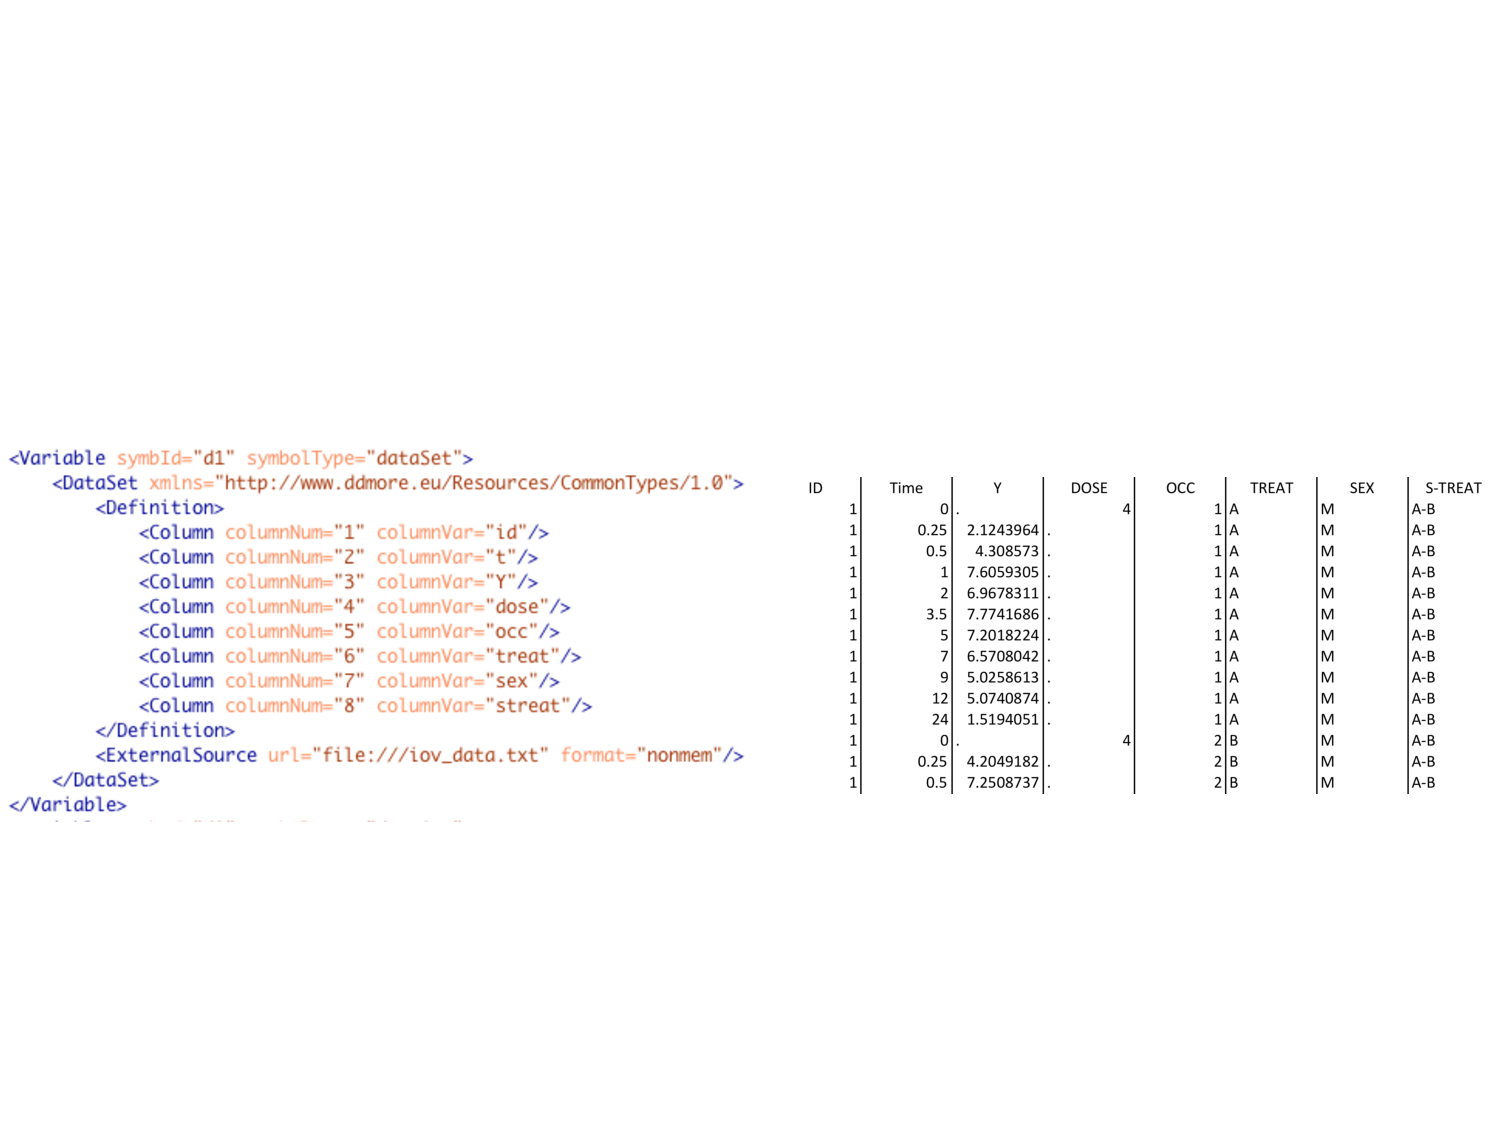
\includegraphics[width=\linewidth,clip=true,trim=0 5.2cm 0 7.5cm]{FirstDatasetExample}
%   \caption{An example of a dataset that corresponds to the contents
%     of a file on the right. Note how the column names in the file are
%     \emph{not} identical to those of the dataset definition. It is the
%     \xatt{columnNum} attribute that determines which column in the
%     file is mapped to which dataset column. }
%   \label{fig: dataset1-eg}
% \end{figure*}

As usual the simplest way to explain it is to look at an example, such
as the code snippet below:
%
\begin{xmlcode}
<ds:DataSet>
    <ds:Definition>
        <ds:Column columnId="id" valueType="string" columnNum="1"/>
        <ds:Column columnId="arm" valueType="string" columnNum="2"/>
        <ds:Column columnId="reps" valueType="int" columnNum="3"/>
    </ds:Definition>
    <ds:Table>
        <ds:Row>
            <ct:String>i1</ct:String><ct:String>a1</ct:String><ct:Int>20</ct:Int>
        </ds:Row>
        <ds:Row>
            <ct:String>i2</ct:String><ct:String>a2</ct:String><ct:Int>20</ct:Int>
        </ds:Row>
        <ds:Row>
            <ct:String>i3</ct:String><ct:String>a3</ct:String><ct:Int>40</ct:Int>
        </ds:Row>
        <ds:Row>
            <ct:String>i4</ct:String><ct:String>a4</ct:String><ct:Int>40</ct:Int>
        </ds:Row>
    </ds:Table>
</ds:DataSet>
\end{xmlcode}
%
As before the dataset has a definition, where the columns of the
dataset table are defined. The column number must start at 1 and each
column must be numbered in consecutive order (i.e.\xspace
1,2,3,4\ldots etc.). The type of each column is specified and this
complies with the \pharmml type system.  Next the content of the
dataset is held within the \xelem{Table} element and this consists of
one or more \xelem{Row} elements. Each row must contain an entry for
each column defined. NULL values are indicated by the \xelem{Null/}
element.

This looks like a table in a relational database and indeed this
approach is based on the concept of a relation in relational
theory. Therefore the ordering of rows is not significant. At present
there is no mechanism to define a key on the dataset or columns that
cannot be NULL. It is assumed that such restrictions may be applied when
the dataset is used. For example it is assumed that when mapping
observations in the \xelem{EstimationStep} none of the data is
NULL and that the combination of the time column and that identifying
the individual are unique.

\begin{figure}[htb]
\centering
%\setlength\fboxsep{0pt}
%\setlength\fboxrule{0.5pt}
%\fbox{%
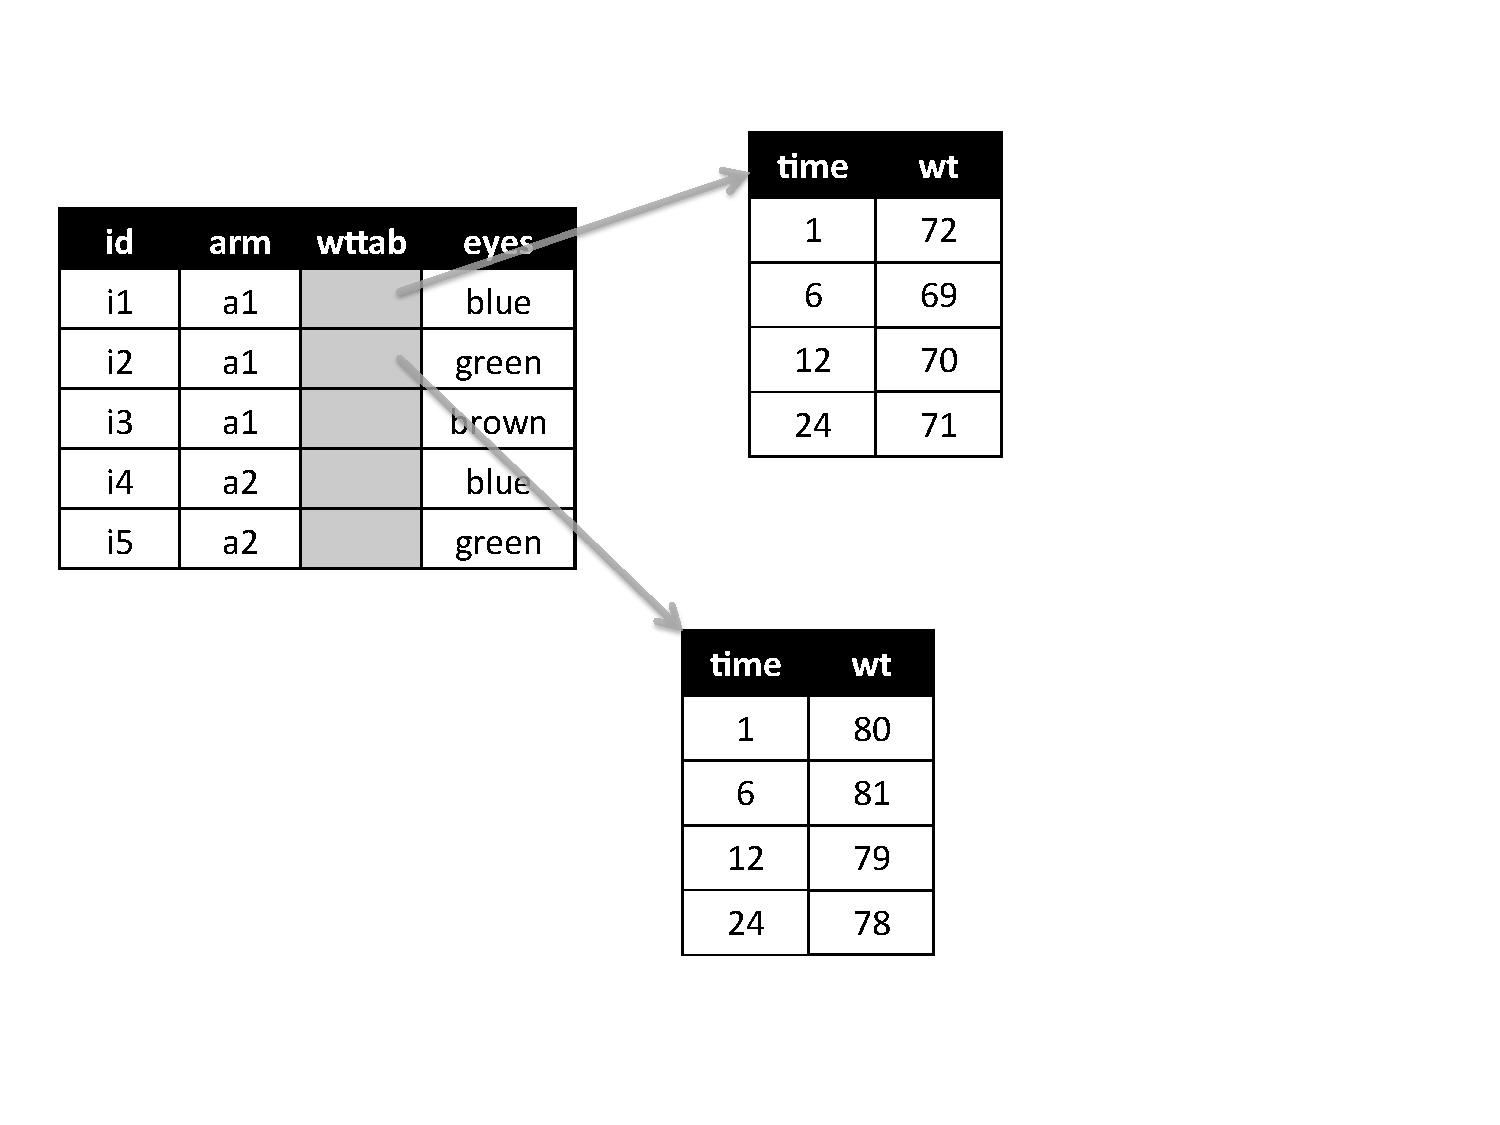
\includegraphics[height=0.35\textheight,clip=true,trim=9mm 1.5cm 8.3cm 2cm]{Datasets}%
%}
\caption{An illustration of how a table with a nested table can be
  conceptualised. Each cell within the \xatt{wttab} column contains
  another table.}
\label{fig:dataset}
\end{figure}

Finally, there is one deviation from standard relational theory in the
dataset. This is that a table can be nested multiple times, i.e., a
table can contain a column that defines another table and so on. This
concept is illustrated in figure \ref{fig:dataset}. We required this
because in some situations it is necessary to define one to many
relationships within the data. For example when defining a population
of individuals in a study whose weight changes during the course of
the study (weight is a time-dependent covariate). In relational theory
this is achieved by a foreign key relationship, but in the dataset it is
simpler and clearer if we take advantage of the hierarchical nature
of the XML. You can see this in the example dataset below:
%
\begin{xmlcode}
<ds:DataSet>
    <ds:Definition>
        <ds:Column columnId="id" valueType="string" columnNum="1"/>
        <ds:Column columnId="arm" valueType="string" columnNum="2"/>
        <ds:Table tableId="wttab" columnNum="3">
            <ds:Definition>
                <ds:Column columnId="time" valueType="real" columnNum="1"/>
                <ds:Column columnId="wt" valueType="real" columnNum="2"/>
            <ds:Definition>
        </ds:Table>
        <ds:Column columnId="eyes" valueType="string" columnNum="4"/>
    </ds:Definition>
    <ds:Table>
        <ds:Row>
            <ct:String>i1</ct:String><ct:String>a1</ct:String>
            <ds:Table>
                <ds:Row>
                    <ct:String>1</ct:String><ct:Real>72</ct:Real>
                </ds:Row>
                <ds:Row>
                    <ct:String>6</ct:String><ct:Real>69</ct:Real>
                </ds:Row>
                <ds:Row>
                    <ct:String>12</ct:String><ct:Real>70</ct:Real>
                </ds:Row>
                <ds:Row>
                    <ct:String>24</ct:String><ct:Real>71</ct:Real>
                </ds:Row>
            </ds:Table>
            <ct:String>blue</ct:String>
        </ds:Row>
        <ds:Row>
            <ct:String>i2</ct:String><ct:String>a1</ct:String>
            <ds:Table>
                <ds:Row>
                    <ct:String>1</ct:String><ct:Real>80</ct:Real>
                </ds:Row>
                <ds:Row>
                    <ct:String>6</ct:String><ct:Real>81</ct:Real>
                </ds:Row>
                <ds:Row>
                    <ct:String>12</ct:String><ct:Real>79</ct:Real>
                </ds:Row>
                <ds:Row>
                    <ct:String>24</ct:String><ct:Real>78</ct:Real>
                </ds:Row>
            </ds:Table>
            <ct:String>green</ct:String>
        </ds:Row>
    </ds:Table>
</ds:DataSet>
\end{xmlcode}
%
In the example the child table is defined by using a \xelem{Table}
element instead of the usual \xelem{Column} element and given the
identifier ``wttab''. Within the nested table definition another set
of columns is specified\footnote{Of course this definition can itself
contain another table definition \emph{ad infinitum}.}. Now when
encoding the data within the dataset its rows are defined as before,
but where a column has been replaced by a nested table the contents of
this table are delimited by a \xelem{Table} element. The dataset in
the example defines individual \texttt{i1} assigned to arm
\texttt{a1} with a weight that varies between $69$ kg and $72$ kg during
the study.

% in figure
% \ref{fig: dataset1-eg}. The \texttt{<DataSet>} element declares that
% what follows is a dataset and the \texttt{<Definition>} element
% defines the columns used by the dataset. Each column is defined by a
% number identifying the column (starting at 1) and is given a name
% (using the attribute \texttt{columnVar}). Both column number and
% column name must be unique within the dataset definition. Finally, the
% source of the dataset is defined. In this case the source is outside
% the \pharmml document (external) and is identified by a URL\@. The format
% of the external resource is also defined, in this case a file in
% \nonmem data format. The comma-separated and tab-delimited formats
% mentioned above are also available.

% \begin{listing*}[htb]
% \inputxml{dataset_internal.xml}
% \caption{Defining dataset data within \pharmml.}
% \label{code:dataset-internal-data}
% \end{listing*}

% In the example (\ref{fig: dataset1-eg}) the variable \attval{d1} is
% initialised with the data in the resource referenced by the
% \xelem{ExternalSource} element (in this case a file). It is important
% to note that unlike \nonmem the names given to each column of the
% dataset is \emph{not} significant. For example, calling a column
% \dscol{TIME} does not imply that this column contains time
% point data. This information is defined later by mapping the
% columns of a dataset to other parts of the \pharmml document
% (c.f.\ section \ref{sec:objective-data-mapping}).

% \begin{listing*}[htb]
% \inputxml{dataset_internal_ref.xml}
% \caption{Creating one dataset from another.}
% \label{code:dataset-internal-ref}
% \end{listing*}

% Data-sets do not need to be sourced from an external source. Their
% data content can be defined within the \pharmml document, as can be seen
% in listing \ref{code:dataset-internal-data}. This illustrates an
% additional concept not seen in the external data source a NULL value,
% encoded by the \xelem{Null} element, which means that no value has
% been provided or exists. This can also be defined by a special
% character in the external data source format, for example in \nonmem
% format the ``.'' indicates no value and so is for our purposes NULL.

% \begin{table}[htb]
% \centering
% \begin{tabular}{r r r r}\toprule
% ID & Time & Y & dose\\\midrule
% 1 & 0 & . & 4 \\
% 1 & 0 & . & 4 \\
% 2 & 0 & . & 4 \\
% 2 & 0 & . & 4 \\
% 3 & 0 & . & 4 \\
% 3 & 0 & . & 4 \\\bottomrule
% \end{tabular}
% \caption{The dataset obtained by selecting a subset of columns
%   from the original dataset and then eliminating all rows where
%   DOSE is NULL.}
%   \label{fig:restricted dataset}
% \end{table}

% A third way to define a dataset is to create it from another, as
% illustrated in listing \ref{code:dataset-internal-ref}. This allows
% you to choose a subset of the original dataset. As you can see this
% can be done in two ways: by selecting a subset of the columns from the
% original dataset or by choosing a subset of its rows based on some
% logical criteria (in \pharmml this is called a \emph{restriction}). In
% the example we are excluding all rows except those with a dosing value
% defined (i.e.\xspace where the column value is not NULL). This allows
% us to extract the dataset in figure \ref{fig:restricted dataset} from
% the original dataset shown in figure \ref{fig: dataset1-eg}.


\section{Mathematical expressions}
\label{sec:maths}
Mathematical expressions are a fundamental part of a pharmacometric
model and so it was important that \pharmml incorporated the
ability to encode these. The question we had in designing the language, however, was
what is the best way to do this?  Our initial approach was to reuse an
existing W3C standard called
\mathml\footnote{\url{http://www.w3.org/TR/MathML3/}}, which was
designed to represent mathematical equations on web pages.
Unfortunately, the full \mathml standard is bigger and more complex
than we need: indeed much of the standard focuses on the presentation
and layout of mathematical equations rather than their underlying
meaning\footnote{We should emphasise that his is not a criticism of
\mathml, as this was the problem it was created to solve!}.  This
was also the conclusion reached for similar standards to \pharmml such as
SBML \cite[Section 3.4]{sbmll3v1c},
CellML\footnote{\url{http://www.cellml.org/specifications/cellml_1.1/\#sec_mathematics}}
and \sedml \cite{sedmll1v1}. Their solution to this problem was to use
a subset of the standard that did what they wanted and to develop their
own software to support this subset. In effect they created their own
version of the \mathml standard. This means that the CellML version of
\mathml is not compatible with the \sbml version and so on, and as a
consequence each standard has had to develop its own software
libraries to support their own version of \mathml.

Faced with the same dilemma we considered adopting yet another subset
of \mathml, but decided against it for a number of reasons:
\begin{enumerate}
\item Because \mathml is designed for the presentation of maths its
  basic design is much more complicated than we require.
\item The design of \mathml is such that it is impossible to validate
  whether a sensible mathematical expression has been formed using
  just XML Schema validation\footnote{XML Schema is an XML standard
    that let's you effectively define an object model in XML. The
    benefit of the standard is that it there many tools that can then
    validated automatically whether your XML document conforms to this
    `object model'. We have taken advantage of this technology in
    \pharmml and it has made development of the specification and
    software support much more efficient.}. This is because it uses
  \verb|<apply></apply>| elements to group operands and operators
  together and so a statement such as
  \verb|<apply><divide/><cn>20/<cn></apply>| ($\div 20$) is
  syntactically valid \mathml, but an incomplete mathematical
  expression.
\item Taking a subset of \mathml requires the creation of a new XML
  Schema definition, new tools for validation and is effectively
  creating a new standard. In our view calling this \mathml is
  misleading as each of the \mathml subsets currently used are not the
  same and cannot be exchanged with each other, nor with W3C \mathml
  (see discussion above).
\end{enumerate}
Consequently we created our own mathematics definition, which has the
following design goals:
\begin{enumerate}
\item Have a design that ensured that mathematical expressions
  were syntactically correct --- allowing us to use XML Schema
  validating software to ensure this correctness.
\item Ensure that the maths could handle all mathematical expressions
  we require in \pharmml.
\item Provide logical expressions for use in piecewise functions.
\item Have a simple and concise design that could be easily written by hand
  and also read by a developer --- to facilitate testing.
\end{enumerate}

Our design follows that of many programming languages, such as C
\cite{Kernighan:1988:CPL:576122}, by defining unary and binary
operators that take one or two operands respectively. Such operands
can be literal values (e.g.\xspace numbers), variables or another
operator. In languages such as C, mathematical expressions are
designed to be easily read by humans, but in \pharmml we don't have
this restriction and we are more interested in ease of computational
processing. For this reason we have adopted a prefix representation.

%\begin{listing*}[htb]
% \inputxml{basic_maths_eg.xml}
% \caption{A simple equation encoded in \pharmml Maths. It
% is equivalent to the expression $(9 - 5) \times 2$.}
% \label{code:math-eg}
% \end{listing*}

In a prefix representation, also called Polish notation\footnote{For
  more information see
  \url{http://en.wikipedia.org/wiki/Polish_notation}.}, the operator is
placed before its operands. We can illustrate this using the following
expression, $(9 - 5) \times 2$, becomes $\times-9\,5\,2$. This is
evaluated from left to right. You first evaluate the operator which
has operands that are numerical values. The result of this operator is
then used as an operand of another operator and the process is
repeated until all operators are evaluated. Using the expression above
as an example: $-9\,5$ is evaluated first that then reduces the
expression to $\times 4\,2$, until finally we are left with the result
of $2$. The benefits for the parser are obvious because we no longer
require grouping constructs like parenthesis. As can be seen in the
following listing, this prefix approach fits well with XML and allows
us to express the above expression concisely\footnote{In fact the XML
  structure actually defines the abstract syntax tree of the
  mathematical expression, which is typically the output of a language
  parser.}.
%
\begin{xmlcode}
<!-- (9 - 5) * 2 -->
<Equation xmlns="http://www.pharmml.org/2013/03/Maths"/>
    <Binop op="times">
        <Binop op="minus">
            <ct:Real>9</ct:Real>
            <ct:Real>5</ct:Real>
        </Binop>
        <ct:Int>2</ct:Int>
    </Binop>
</Equation>
\end{xmlcode}
%
It also allows us to use XML Schema validation to ensure correctness
because we can validate that all binary operators require two operands
and a unary operator one. The more complicated example below shows how
to define the expression $\exp\left(-\textrm{logit}(i) + \beta
  \ln\left(\frac{W}{70}\right)+\eta\right)$ with unary and binary
operators:
\begin{xmlcode}
<?xml version="1.0" encoding="UTF-8"?>
<Equation xmlns="http://www.ddmore.eu/Resources/Maths/1.0"/>
    <!-- Omitted namespace declarations -->
    <Uniop op="exp">
        <Binop op="plus">
            <Uniop op="minus">
                <Uniop op="logit">
                    <ct:SymbRef symbIdRef="i"/>
                </Uniop>
            </Uniop>
            <Binop op="plus">
                <Binop op="times">
                    <ct:SymbRef symbIdRef="beta"/>
                    <Uniop op="ln">
                        <Binop op="divide">
                            <ct:SymbRef symbIdRef="W"/>
                            <ct:Real>70</ct:Real>
                        </Binop>
                    </Uniop>
                </Binop>
                <ct:SymbRef symbIdRef="eta"/>
            </Binop>
        </Binop>
    </Uniop>
</Equation>
\end{xmlcode}

Besides mathematical expressions \pharmml Maths can also define logical
expressions used in conditional logic that enables us to define
piecewise functions. %
% and these conditions can be used independently in
%the manner of an SQL WHERE clause (c.f.\xspace section
%\ref{sec:dataset}).
This uses the same postfix approach, but with alternate logical binary
and unary operators defined by the \xelem{LogicBinop} and
\xelem{LogicUniop} elements, respectively. The following example shows
how it can be combined with mathematical expressions to describe the
piecewise expression:
%
\[
\begin{cases}
-x & \text{if } x < 0\\
 x & \text{if } x \geq 0
\end{cases}
\]
%
Note that because logical expressions can contain strings it is
possible to define such expressions using non-numerical criteria:
%
\begin{xmlcode}
<Equation xmlns="http://www.ddmore.eu/Resources/Maths/1.0"/>
    <!-- Omitted namespace declarations -->
    <Piecewise>
        <Piece>
            <Uniop op="minus">
                <ct:SymbRef symbIdRef="x"/>
            </Uniop>
            <Condition>
                <LogicBinop op="lt">
                    <ct:SymbRef symbIdRef="x"/>
                    <ct:Int>0</ct:Int>
                </LogicBinop>
            </Condition>
        </Piece>
        <Piece>
            <ct:SymbRef symbIdRef="x"/>
            <Condition>
                <LogicBinop op="geq">
                    <ct:SymbRef symbIdRef="x"/>
                    <ct:Real>0</ct:Real>
                </LogicBinop>
            </Condition>
        </Piece>
    </Piecewise>
</Equation>
\end{xmlcode}

A complete list of the mathematical and operators that are available
is provided in section~\ref{sec:phmaths-defns}.  Here you will also
find a description of each operator's semantics and the permitted types
of its operands.

\section{Representing statistics}

As can be seen in chapter \ref{chap:mathsdefn}, \pharmml relies on the
ability to use probability distributions to describe the variability
in a pharmacometric model. Admittedly, the most commonly used
distribution is the normal distribution (or transformations of it),
but our intention is that \pharmml will have the flexibility to
describe a wide range of probability distribution types. To do this
the languages uses \uncertml version
3\footnote{\url{http://www.uncertml.org}}, which is an XML Schema
based language that aims to ``describe and exchange
uncertainty''. UncertML supports all the commonly used continuous and
discrete probability distributions and so more than adequately
supports the needs of \pharmml.  As an example we can show how the
normal distribution $\mathcal{N}(0, \omega^2)$ can be defined in
\uncertml.
% shown in listing \ref{code:normal-dist-eg}.
\begin{xmlcode}
<NormalDistribution xmlns="http://www.uncertml.org/3.0"
    definition="http://www.uncertml.org/distributions/normal">
    <mean><rVal>0</rVal></mean>
    <stddev><var varId="omega"/></stddev>
</NormalDistribution>
\end{xmlcode}

% \begin{listing*}[htb]
% \inputxml{normal.xml}
% \caption{XML code encoding the normal distribution, $\mathcal{N}(0,
%   1)$.}
% \label{code:normal-dist-eg}
% \end{listing*}


% \section{Representing the Structural Model}

% In \pharmml one of our aims has been to reuse existing standards where it
% makes sense to do so. One standard that is suited for this purpose is
% \sbml. It can be used to encode systems of ODEs or algebraic
% equations, but it can also encode more complicated mechanistic models
% too. For example models that describe signalling pathways spanning
% multiple compartment. Therefore, it is our preferred mechanism for
% representing the structural model in \pharmml.

% However, in order to use a structural model encoded in \sbml we need
% to somehow incorporate it into the \pharmml document. We do this with the
% \xelem{Import} element as can be seen in listing
% \ref{code:import-eg}. In doing so the import statement maps equivalent
% variables in the \pharmml document to those in the \sbml model.

% \begin{listing*}[htb]
% \inputxml {sbml-import1.xml}
% \caption{This snippet illustrates how we map the parameters
%   and variables in the \pharmml document to the \sbml model. The model
%   itself is identified by a URL and the type of model is identified as
% \attval{sbml}. The variables and the parameters (not shown) in the
% \pharmml document are mapped to those in the \sbml model.}
% \label{code:import-eg}
% \end{listing*}

% In addition to incorporating \sbml models we can also incorporate
% other structural models defined in \pharmml. This mechanism is there for
% completeness and is not the preferred method for including models,
% so we will not go into in more detail here.

\section{Time}
\label{sec:independent-var}

Time is required by most pharmacometric models and in \pharmml it can
be referred to explicitly. The symbol used for the time variable is
configurable at the beginning of the document as shown below:
%
\begin{xmlcode}
<PharmML xmlns="http://www.pharmml.org/2013/03/PharmML"
    xmlns:xsi="http://www.w3.org/2001/XMLSchema-instance"
    xsi:schemaLocation="http://www.pharmml.org/2013/03/PharmML ..."
    xmlns:math="http://www.pharmml.org/2013/03/Maths"
    xmlns:ct="http://www.pharmml.org/2013/03/CommonTypes"
    xmlns:ds="http://www.pharmml.org/2013/08/Dataset"
    xmlns:design="http://www.pharmml.org/2013/03/TrialDesign"
    writtenVersion="0.1">
    <ct:Name>IOV1 with covariates</ct:Name>
    <IndependentVariable symbId="t"/>
\end{xmlcode}
%
%(see listing \ref{code:indep-var-eg}).
Rather than time we call the element \xelem{IndependentVariable}
because this is more correct and because you could define a model that
uses another quantity than time as the independent variable (e.g.\xspace
dose in a dose-response model). Note that the independent variable
always has a real type.

% \begin{listing*}[htb]
% \inputxml{indep_var_eg.xml}
% \caption{{In this code snippet the independent variable is defined as $t$.}}
% \label{code:indep-var-eg}
% \end{listing*}

% \section{Units}
% \label{sec:units}

% \pharmml allows you to specify the units of the quantities in a
% model. This may seem like a trivial thing to do, but when such
% quantities are incorporated into equations (as they are here)
% then we need to take steps to ensure units are consistent with each
% other. That is, we need to check that the dimensions on the left hand side of an
% equation match those on the right and that the units have the same
% scale. For example it should recognised that $1000$ and $1kg$ are
% equivalent as are $0^o C$ and $32^o F$.

% The other issue is what units to support? Clearly the number of
% possible units is large and trying to predefine all possible units
% will be a cumbersome task. Instead we have borrowed the approach used
% by SBML \cite[Section 4.4]{sbmll3v1c} where units are defined using a
% set of basic units\footnote{Our approach varies slightly from that of
%   SBML in that we strick to a minimal set of base units and we allow
%   unit definitions to be built up from other unit definitions.}. These
% `built-in' units cover all dimensions and can be used to build up any
% specific unit. For example we may have a $g$ as the fundamental unit
% of mass and then define a $kg$ which is a gram scaled by 1000. An
% example of what it might look like is below:
% %
% \begin{xmlcode}
% <UnitDefinition symbId="hour">
%     <Symbol>h</Symbol>
%     <Unit basicUnit="second">
%         <Exponent>1</Exponent>
%         <Scale>0</Scale>
%         <Multiplier>3660</Multiplier>
%     </Unit>
% </UnitDefinition>
% \end{xmlcode}
% %
% As you can see, the \xelem{UnitDefinition} element defines the unit in
% terms of a base unit referred to in the \xelem{Unit} element.  The
% \xelem{Unit} element describes the conversion of the base unit a
% consistent of the unit being defined. This defines the unit
% $mathit{hour}$ as $(3660 \cdot 10^0 \cdot \mathit{second})^1$: in
% otherwords 1 hour is 3600 seconds.  The base units used in \pharmml
% are the seven base units from SI\footnote{See Section 2 in
%   \url{http://http://www.bipm.org/utils/common/pdf/si_brochure_8.pdf}.}
% plus a dimensionless unit (see section~\ref{sec:base-units-defn}). The
% components of the definition are then combined in the following
% equation:
% %
% \[
% \mathit{unit} = \left(\mathit{multiplier} \cdot 10^{\mathit{scale}}
%     \cdot \mathit{baseunit} \right) ^{\mathit{exponent}}
% \]
% %
% More complex units can contain multiple \xelem{Unit} elements:
% %
% \begin{xmlcode}
% <UnitDefinition symbId="velocity">
%     <ct:Symbol>ms-1</ct:Symbol>
%     <Unit basicUnit="metre">
%         <Exponent>1</Exponent>
%     </Unit>
%     <Unit basicUnit="second">
%         <Exponent>-1</Exponent>
%     </Unit>
% </UnitDefinition>
% \end{xmlcode}

% Combining unit definitions effectively multiplies then so above we
% define velocity as $ms^{-1}$. Note that if the \xelem{Scale} and
% \xelem{Multiplier} elements are omitted they are assumed to be 0 and 1
% respectively. The example below shows how we might use these
% definitions, for example to define the time units used in the model:
% %
% \begin{xmlcode}
% <IndependentVariable symbId="t">
%     <Units symbId="hour"/>
% </IndependentVariable>
% \end{xmlcode}

% Note also that derived units can be composed from other derived
% units as shown below, where the unit $mg$ is first derived from the
% base unit kilogram as $(1 \cdot 10^-3 \cdot kg)^1$ and the unit $mg/kg$ is
% derived as a combination of $(1 \cdot 10^0 \cdot kg)^-1$ and $(1
% \cdot 10^0 \cdot kg)^1$.
% \begin{xmlcode}
% <ct:UnitDefinition unitId="mg">
%     <ct:UnitComponent>
%         <ct:BasicUnitRef basicUnit="kilogram"/>
%         <ct:Exponent>1</ct:Exponent>
%         <ct:Scale>-4</ct:Scale>
%     </ct:UnitComponent>
% </ct:UnitDefinition>
% <ct:UnitDefinition unitId="mg_kg-1">
%     <ct:UnitComponent>
%         <ct:UnitRef unitId="mg"/>
%     </ct:UnitComponent>
%     <ct:UnitComponent>
%         <ct:BasicUnitRef basicUnit="kilogram"/>
%         <ct:Exponent>-1</ct:Exponent>
%     </ct:UnitComponent>
% </ct:UnitDefinition>
% \end{xmlcode}

% In this version of \pharmml unit definitions are optional and unit
% consistency is not be enforced. In other words there is no validation
% rule stating that units must be consistent. The aim is to first
% establish the structures to define units within the specification and
% then at a future date to add rules about unit consistency. Why not
% now? Largely pragmatism. Unit consistency can only be enforced if all
% quantities in the \pharmml document use them, so to make such
% consistency mandatory will put a burden on tool developers. We would
% prefer to defer this decision until we have all gained experience using
% units in \pharmml.

\section{Element identifier}
\label{sec:element-id}

We know that other resources will wish to interact with \pharmml and
so we have given some thought to how best they should refer to
specific pieces of information in a \pharmml document. Our solution is
to provide every XML element in the document with an optional unique
identifier. The listing below shows how the \xatt{id} attribute is
used:
%
\begin{xmlcode}
<FixedEffect id="e10" symbId="beta_V">
    <Covariate>
        <ct:SymbRef  symbIdRef="W"/>
    </Covariate>
</FixedEffect>
<FixedEffect id="e13" symbIdRef="beta_Cl">
    <Covariate>
        <ct:SymbRef symbIdRef="W"/>
    </Covariate>
</FixedEffect>
<RandomVariable id="e16" symbId="eta_V">
    <ct:VariabilityReference id="e17">
        <ct:SymbRef id="e18"  blkIdRef="model" symbIdRef="level"/>
   </ct:VariabilityReference>
   <!-- Snip -->
</RandomVariable>
\end{xmlcode}
%
As you can see the \xatt{id} attribute is optional and need only be
used for elements that you want to refer to. There are no rules other
than that the identifier must be unique within the \pharmml document.
Thus to refer to a specific part of a document all you need to define is
the location of the document and the identifier. So assuming that the
above code snippet is found in a file called ``testFile.xml'' a
suitable (relative) URI that refers to the random variable in the
example might be \url{testFile.xml#e16}.

The benefit of this approach is that the \xatt{id} attribute can
easily be made available programmatically and searched on with a class
library generated from the XML Schema.
%\footnote{We considered using the XPath
% standard\cite{xpath} to identify elements using what is in effect an
% XMl query language, but we felt that it would be very difficult to
% execute such queries on a class library encode in a programming
% language the query is on the XML not attributed help within the prograsuch as
% Java, which is what you would need to do when interacting with
% \pharmml via the libPharmML API (see section
% \ref{sec:libpharmml}).
This mechanism is also used successfully by SBML \cite[Section
6]{sbmll3v1c}. You will see in the sections below (sections \ref{sec:annotation} and
\ref{sec:extension}) how we take advantage of this mechanism to
annotate and extend a \pharmml document.

\section{Ordering modelling steps}

Descriptions in a modelling step are declarative, describing what
was done, what algorithms were used and what their properties were.

\begin{figure}[htb]
 \centering
  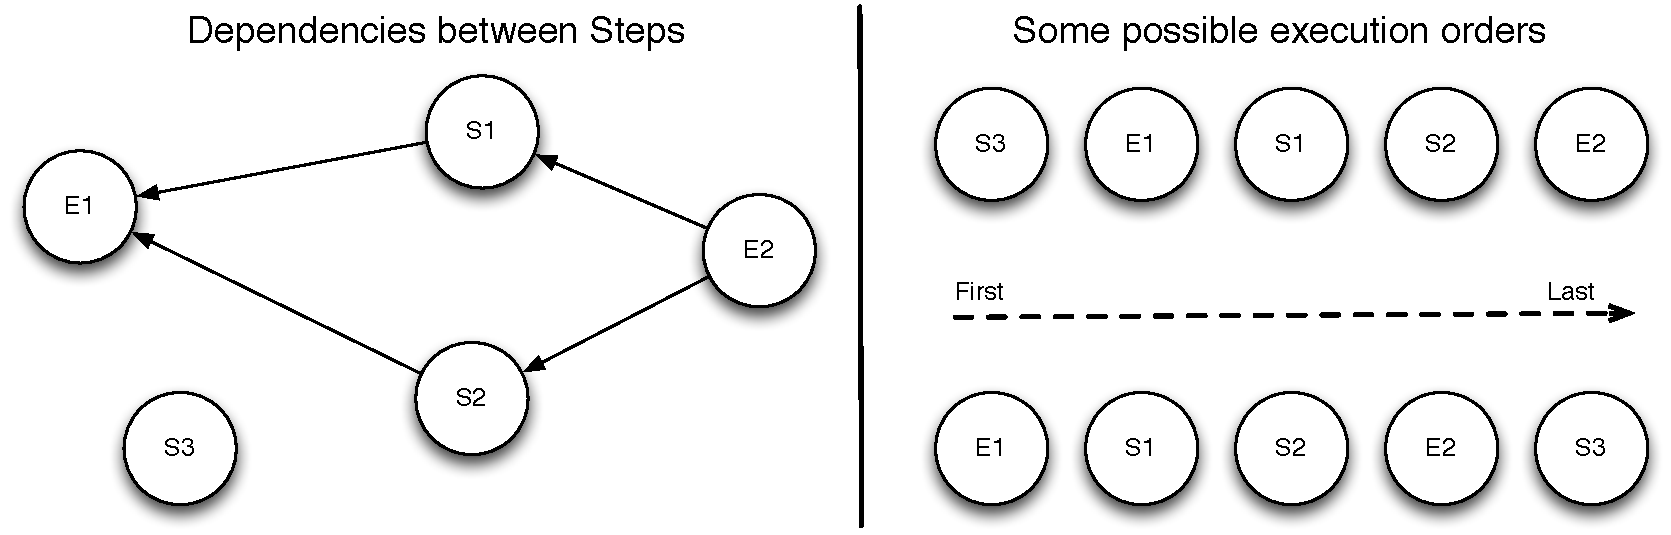
\includegraphics[width=1\linewidth]{ModellingStepDeps}
  \caption{An example of the dependencies between modelling steps is
    shown on the left. The arrow indicates the direction of the
    dependency so step S1 is dependent on the successful completion of
    step E1. So in this example step E1 must be executed before step
    S1 and S2, and those steps must both execute before step E2. On
    the right-hand figure we show two possible execution orders that
    correspond to the task dependecies on the left. It is important to
    remember that, as in this example, there can be more than one
    execution order for a given set of task dependencies.}
  \label{fig:modellingstep_deps}
\end{figure}

The \phsec{Modelling Steps} section has two components that describe
simulation or estimation tasks. Multiple tasks can be linked together so
that a given estimation task can be placed before a given simulation
task or no order can be given in which case tasks can be executed in
parallel or in any order. A task is ordered by defining its dependent
tasks: tasks that must complete successfully before it can start (see
figure~\ref{fig:modellingstep_deps}). In this way the modelling steps
make no assumptions about how or where its tasks are executed, but
provides enough information for a workflow engine to parallelise the
execution of its tasks successfully, should it wish to.

At the moment tasks cannot specify how output is generated from either
an Estimation or Simulation step. A result of this restriction is that
it is \emph{not} possible to exchange information from one modelling
step to another: for example to use the output of an estimation to set
the parameter values in an estimation. We recognise that this is a
limitation of the current version and this functionality will be
provided in a future release of \pharmml.


\section{Supporting Resources}
\label{sec:supporting-res}

\subsection{Metadata: annotating the \pharmml document}
\label{sec:annotation}

As has been stated above (Chapter \ref{chap:scope}), the purpose of
the \pharmml document is to provide a mathematical and structural
description of a pharmacometric model, sufficient for it to be
executed. Additional information, such as a description of the disease
process being modelled, the exact estimation algorithm or a
publication describing the model is not included in the \pharmml
document. Typically called metadata,
%\footnote{Metadata mean data about
  % data and is correctly used when referring to data that defines other
  % data: such as the definition of a relational database schema. In
  % this field metadata is the commonly used term for what may be more
  % accurately called annotation. However in the specification we have
  % followed convention and use the term metadata in this context.},
this information is still very important and so \pharmml aims to
provide support for external annotation.

\begin{figure}[htbp]
\centering
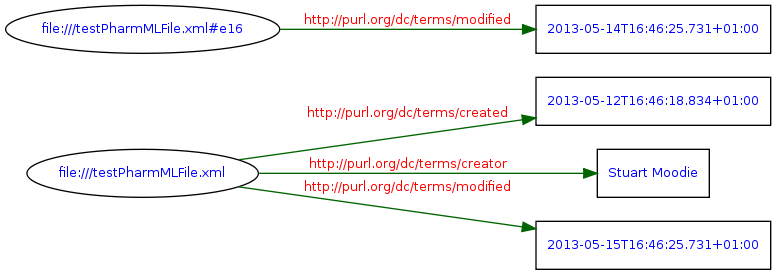
\includegraphics[width=0.8\linewidth]{rdf_graph}
\caption{This figure illustrates how information in the RDF example is
organised. Simply put the subject of the annotation is on the left and
is annotated by the object on the right. The meaning of that
annotation is described by the \emph{predicate} term labelling the
arrow. So reading the top subject from left to right we understand that
element \emph{e16} was \emph{modified} at \emph{14/05/13 at 4:46pm}.}
\label{fig:rdf-graph}
\end{figure}

We expect such metadata to take the form of ontological annotation and
while the detail of what will be annotated is out of scope of this
document we can show how this can work using a standard for describing
resources (such as XML documents) called Dublin Core\footnote{For more
  information see \url{dublincore.org}.}. Using this ontology we can
describe many things about a \pharmml document such as when and by
whom it was created or last updated. Typically such annotation is
expressed using a standard called RDF\footnote{See RDF URL}, which can
be updated and queried using associated software libraries. The
following example\footnote{This example is available as part of the
  examples provided with this specification at
  \texttt{examples/\-CombineArchive/\-annotation.xml}.} gives you a
flavour of what an RDF annotation of a \pharmml document would look
like if we were referring to the code snippet in
section~\ref{sec:element-id}.
%
\begin{xmlcode}
<rdf:RDF
    xmlns:rdf="http://www.w3.org/1999/02/22-rdf-syntax-ns#"
    xmlns:dcterms="http://purl.org/dc/terms/">
  <rdf:Description rdf:about="testPharmMLFile.xml">
    <dcterms:created>2013-05-12T16:46:18.834+01:00</dcterms:created>
    <dcterms:creator>Stuart Moodie</dcterms:creator>
    <dcterms:modified>2013-05-15T16:46:25.731+01:00</dcterms:modified>
  </rdf:Description>
  <rdf:Description rdf:about="testPharmMLFile.xml#e16">
    <dcterms:modified>2013-05-14T16:46:25.731+01:00</dcterms:modified>
  </rdf:Description>
</rdf:RDF>
\end{xmlcode}
%
The metadata above is encoded in RDF-XML\footnote{See \url{rdf-xml}}
and annotates two things. The first \xelem{rdf:Descr\-iption}
element states when the file was both created and modified and also
who created it. The second \xelem{rdf:Description} element points to
the XML element in the PharmML document with an \xatt{id} value of
``e16''. In the example in section \ref{sec:element-id} this is the
\xelem{RandomVariable} element and so we can deduce that this
description is telling us when this element was modified.
Another way of looking at RDF information is shown in figure
\ref{fig:rdf-graph}, which hopefully makes the relationships described
above even clearer. Of course this is a trivial example, but it
illustrates how the \pharmml document can be annotated using metadata
described in a separate RDF document.


\subsection{Standard Structural Models}

In many, if not the majority, of pharmacometric models the structural
model is selected from a standard library. Modelling tools such as
\nonmem or \monolix provide large platform specific libraries
\cite{NONMEM:2006aa} \cite{Bertrand:2008}. These have the benefit of
being both reusable and optimised to run efficiently on their target
platform. With \pharmml we want to support both of these features and
so we will be establishing a framework that provides the following:
\begin{description}
\item[a model ontology] an ontology describing all the models held in
  the standard library.
\item[tool specific mappings] using the model ontology this will
  provide mapping from the models in the standard library to tool
  specific models.
\end{description}

\begin{figure}[htb]
\centering
  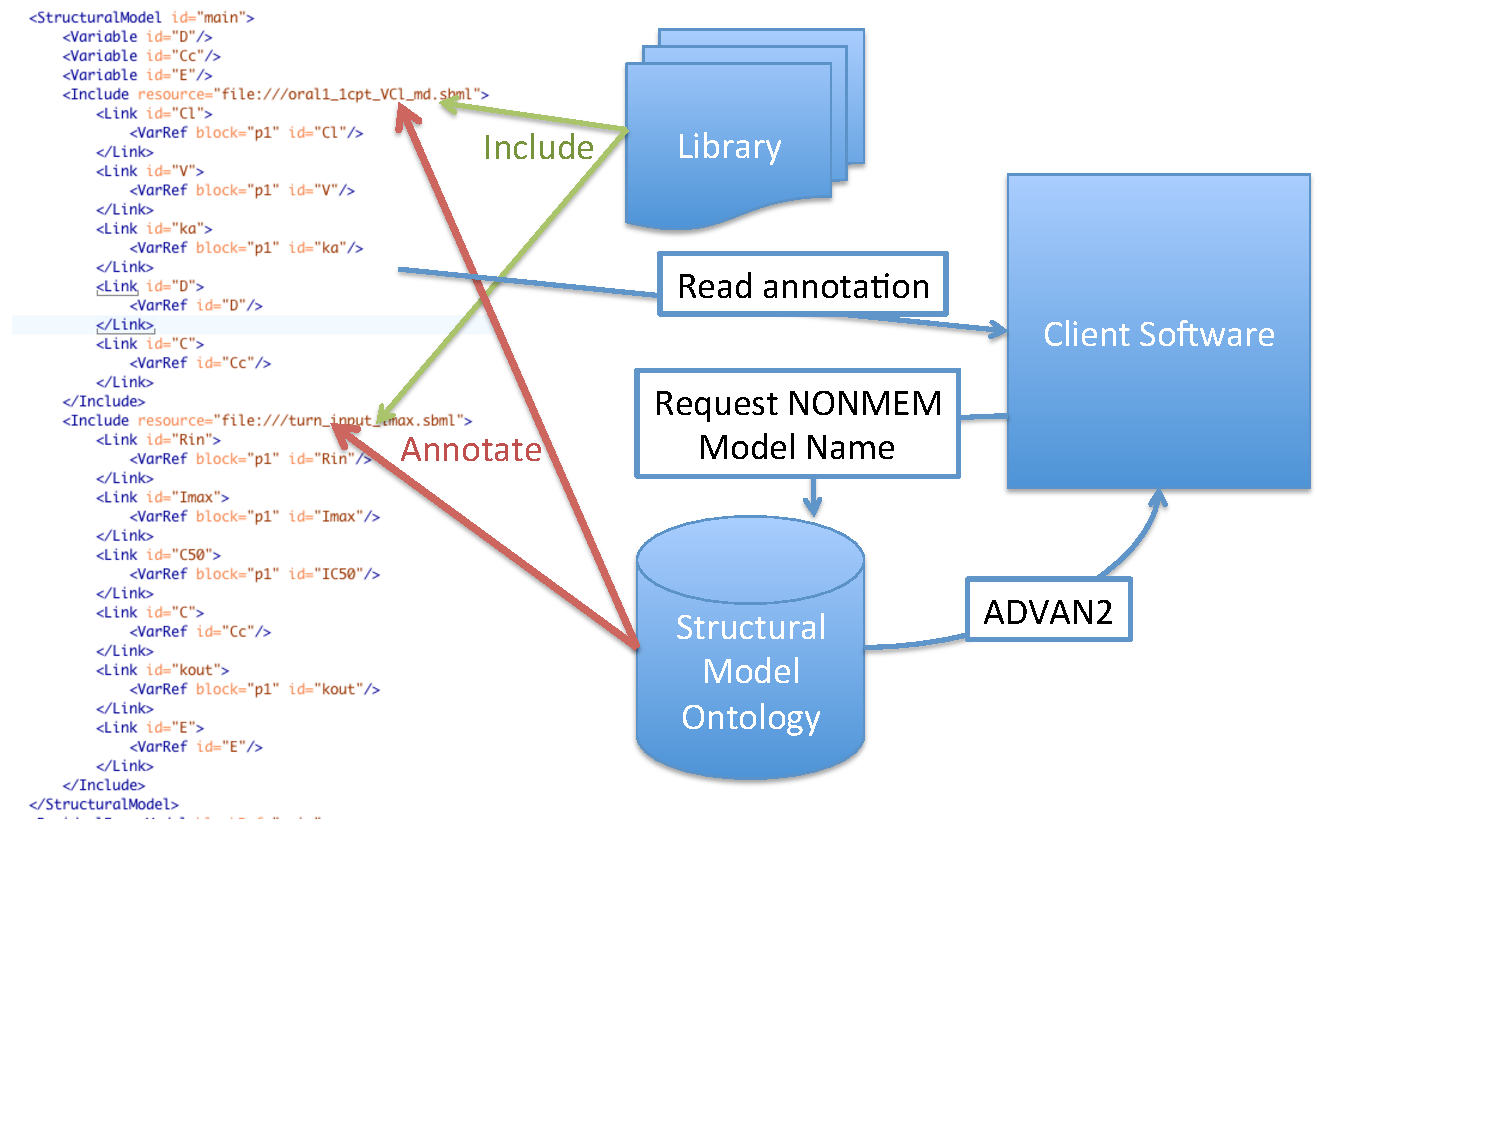
\includegraphics[width=0.9\linewidth,clip=true,trim=0cm 5.5cm 3.5cm 0cm]{ModelMapping}
  \caption{A schematic diagram illustrating how the standard library
    ontology framework is used to generate target specific code when
    translating \pharmml for a specific M\&S tool.}
  \label{fig:model-mapping}
\end{figure}

We expect that the structural model within the \pharmml document will
be annotated with the correct structural model using the model
ontology (following the annotation mechanism described above in
section~\ref{sec:annotation}).  The model ontology term can be used to
identify the appropriate model name for a given modelling tool by
using one of the tool-specific mappings. This allows \pharmml to
provide a tool-independent description of standard structural models.
It also allows conversion tools to convert a \pharmml model into a
tool specific encoding that takes advantage of its built-in structural
model library. This process is summarised in
figure~\ref{fig:model-mapping}.

\subsection{Extending PharmML}
\label{sec:extension}

As with any standard there will be circumstances when it does not
represent all the information that you would like and it would be
convenient to extend it. Typically there are two scenarios where this
is likely to be the case. The first is when the information is genuinely
not supported by \pharmml. This may be because it has not been
implemented yet, or it may be that there is no consensus about whether
this information should be included or no agreement about the best way
to represent it. The second scenario is when you want to
add application specific information to a \pharmml document. Perhaps
because a tool wishes to use \pharmml as its native storage format in
which case it would also want to store information about application
settings etc.

Whatever the reason \pharmml can be extended. Like the metadata
descriptions above (section \ref{sec:annotation}) this approach relies
on the element identifier (see section~\ref{sec:element-id}). The
recommended approach is that you develop a separate XML document
(typically in a separate file), which we will call the extension
document, using any XML representation you choose. Where information
in the extension document relates to the content of the \pharmml
document then you can refer to the relevant XML element using its
identifier.

\begin{figure}[htb]
\centering
  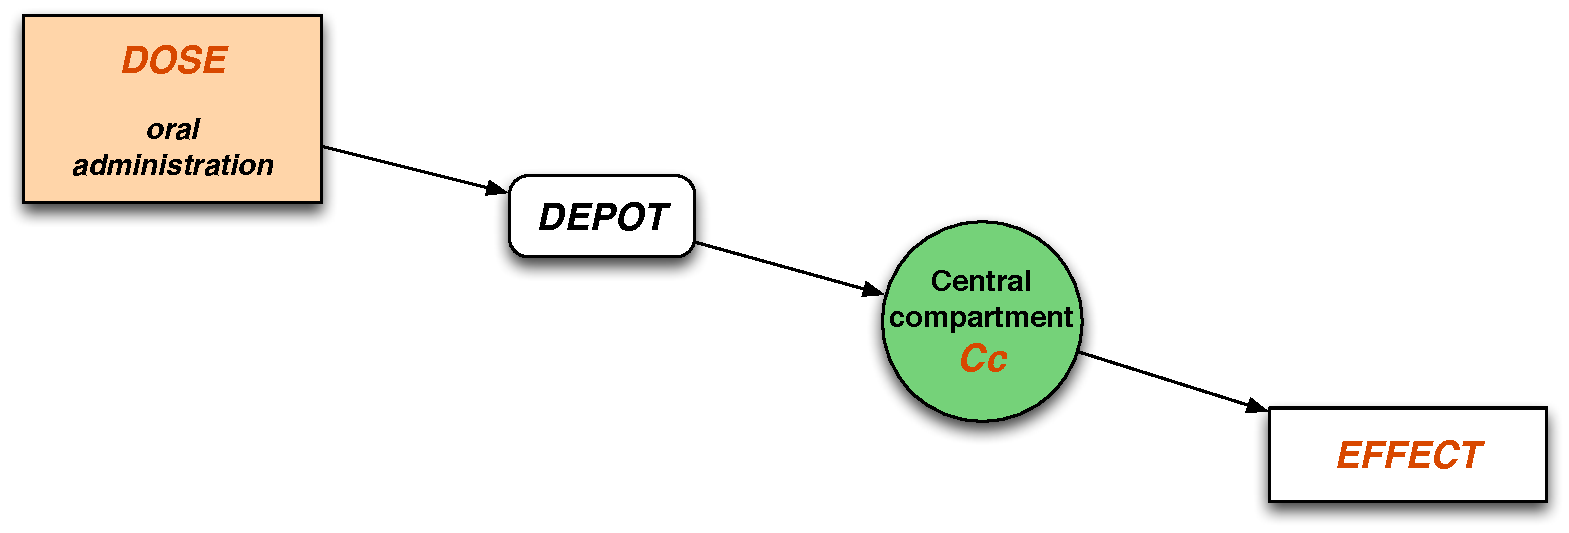
\includegraphics[height=0.2\textheight]{GraphicalModel}
  \caption{This diagram is reproduced from an example in the Monolix
    user manual \cite{Monolix4.1.4UserGuide:2012} and it provides a
    graphical description of a structural model. In the hypothetical
    example in the text we illustrate how you might extend \pharmml to
    link this graphic with the components of the model it represents.}
\label{fig:graphical-model}
\end{figure}

We can illustrate with an example based on the second scenario we
described above: application specific extensions. In this scenario our
software tool provides a graphical interface that lets you create a
pharmacometric model by drawing and connecting shapes such as the
diagram in figure~\ref{fig:graphical-model}. When you save the diagram
the application saves both the \pharmml that encodes the model and an
extension document that describes the graphical layout and maps the
graphical elements to the relevant parts of the model. The extension
document could look like this:
%
\begin{xmlcode}
<?xml version="1.0" encoding="UTF-8"?>
<Diagram resource="file:///anotherPharmMLFile.xml">
    <Rectangle id="1">
        <Name>Dose</Name>
        <Bounds x="10" y="10" w="50" h="30"/>
        <!-- Omitted other information such as colour and other text-->
        <Ref idRef="e35"/>
    </Rectangle>
    <!-- Omitted -->
    <Circle id="3">
        <Name>Central</Name>
        <Bounds x="10" y="200" w="45" h="45"/>
        <!-- Omitted other information such as colour and other text-->
        <Ref idRef="e46"/>
    </Circle>
    <!-- Omitted other shape definitions-->
    <Link src="1" tgt="2"/>
    <Link src="2" tgt="3"/>
    <Link src="3" tgt="4"/>
</Diagram>
\end{xmlcode}
%
The XML describes the shapes of the nodes, their location and the
connections between them. What allows it to extend the \pharmml document?
First the \xatt{resource} attribute provides a URL describing
the location of the \pharmml document being extended. Next the
\xelem{Ref} element defines a reference that points to an element in
the \pharmml document. From this information the application is able
to read both the \pharmml and the extension documents and then relate
the diagram to the relevant part of the model.

Note that while this is a hypothetical example for \pharmml, this type
of solution has been implemented by a graphical Systems Biology editor
called CellDesigner\footnote{\url{www.celldesigner.org}}. It uses SBML
as its native application format: encoding the model in SBML and using
SBML's extension facilities to store graphical information and other
application specific properties.

One final clarification. The extension mechanism does not require an
application to use the same XML elements as described in the example
above. The XML content of the extension document is entirely the
concern of the application. In order to extend a \pharmml document
all it must do is:
\begin{enumerate}
\item Specify how to find the \pharmml document. Using a URI is a good
  way to do this.
\item Use the element identifier to refer to the content of the \pharmml document.
\end{enumerate}

\subsection{Organising \pharmml resources}
\label{sec:pharmml-archive}

We expect that \pharmml will in normal usage consist of more than one
file. From the discussion about annotating
(section~\ref{sec:annotation}) and extending
(section~\ref{sec:extension}) \pharmml it is clear that both of these
cases require the creation of resources that are closely
related to a \pharmml document. It is therefore desirable that they
are kept together and exchanged and used together.

\begin{figure}[htb]
\centering
  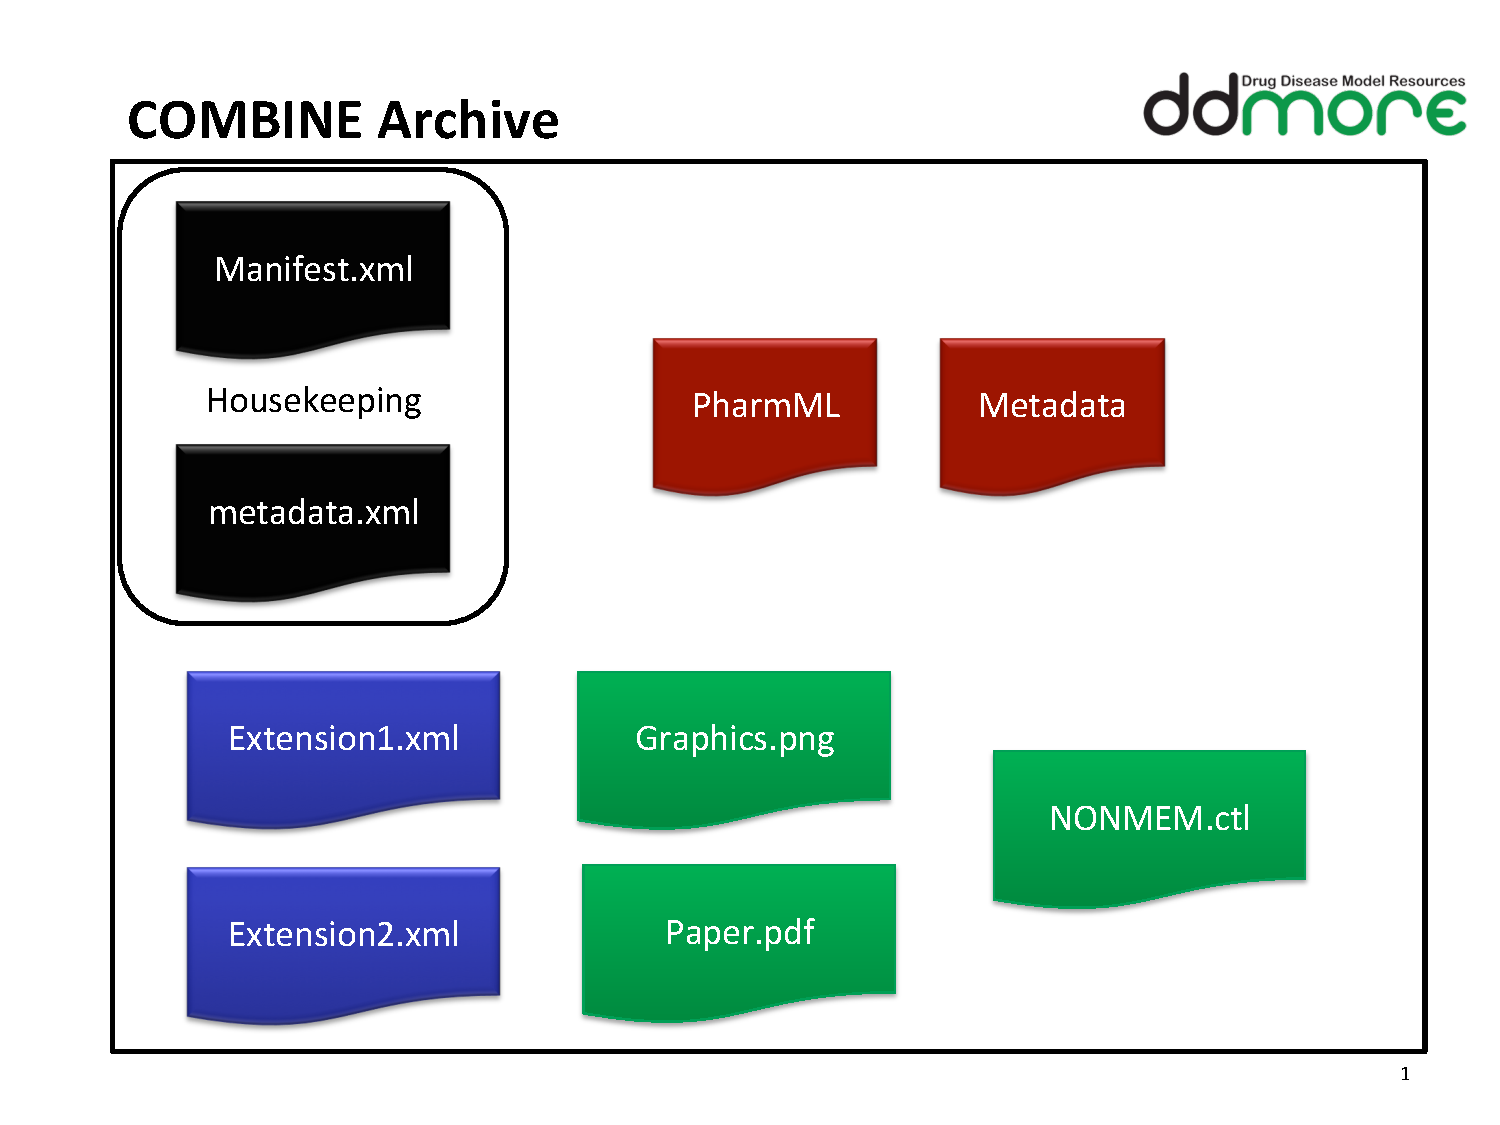
\includegraphics[width=0.6\textwidth]{AchiveOverview}
  \caption{An overview of how a COMBINE archive may be used to hold
    XML documents and files associated with a model encoded in
    \pharmml. In this example the archive holds the model and its
    metadata (in red) and two application specific extension
    documents (in blue). This also shows another advantage of using
    the archive: you can store other useful information, such as the
    original model file, relevant papers or images (in
    green). Finally, the archive contains a metadata file (in black)
    that helps an application reading the archive make sense of what
    it contains.}
  \label{fig:moml-archive-overview}
\end{figure}

An archive file can provide this functionality. It acts as a
container, and since it is a file can be easily exchanged and
stored. We recommend that you use an archive based on the emerging
COMBINE Archive
standard\footnote{\url{http://co.mbine.org/documents/archive}}. It is
based on a zip archive and holds additional information that allows
you to identify the modelling resources in the file. The exact details
of how it works is outside the scope of this document, but the
components of the archive and how it can be used to hold \pharmml
related resources is illustrated in
figure~\ref{fig:moml-archive-overview}\footnote{An example of a
  CombineArchive file that contains a metadata file annotating a
  \pharmml document can be found in \texttt{examples/CombineArchive/archive.zip}.}.

\subsection{Software support for \pharmml}
\label{sec:libpharmml}

\pharmml is a complex language. It is designed using an industry
standard, XML Schema\footnote{\url{http://www.w3.org/XML/Schema}}, which gives us the
ability to use widely available software packages to verify that the
XML file is correctly written and that elements are put in the right
place (syntax checking). However, \pharmml describes a pharmacometric
model and so there is a lot of information that is very specific to
this domain and cannot be validated by standard tools.  That's why we need
\pharmml specific software tools and libraries. Without such software
the burden of validation falls on the modelling tools reading and
writing \pharmml. Given the complexity of \pharmml's validation rules
it is unlikely that such validation would be complete and implemented
consistently, which makes our goal of exchange between modelling
tools less likely to succeed.

Therefore in parallel to the development of this specification a
software library called libPharmML\footnote{For more information see
  the libPharmML specification in the DDMoRe Interface Europe
  document repository: WP2 deliverables: \emph{D2.2
    libPharmMLTechSpec}.} is being developed to support it.  This will
allow you do the following:
%
\begin{enumerate}
\item Create a new \pharmml document.
\item Read an existing \pharmml document from a file (or other
  resource).
\item Write a \pharmml document to a file (or resource).
\item Validate that a \pharmml document complies with the XML Schema
  definition and the rules set out in this specification.
\end{enumerate}
%
The library is implemented in Java. There are no plans to implement an equivalent
version in another programming language, such as C++, but this could be done if
there was sufficient demand for it and sufficient developer resources were available
to implement it.


\chapter{Worked Examples}
\label{chap:worked-egs}

\section{How this chapter is organised}

In developing \pharmml we have found it very useful to explain the
language using examples. By taking you through some pharmacometric models
that you are familiar with we also hope to help you understand how they
correspond to the XML representation in \pharmml. Each example is designed
to illustrate different aspects of \pharmml and our aim is that by the
end of this chapter you will understand the language and what it can
do and --- perhaps equally importantly --- what it cannot do. For
clarity and to save space we will only show key excerpts from the
examples, but the complete examples are available and will be
distributed with this document.

Figure \ref{fig:simEstTasks_List} shows an comparison in the 
structure to be implemented for a typical simulation and estimation task.
Boxes underline elements where the structure of \pharmml for these two tasks differs.

\begin{figure}[htb]
 \centering	
 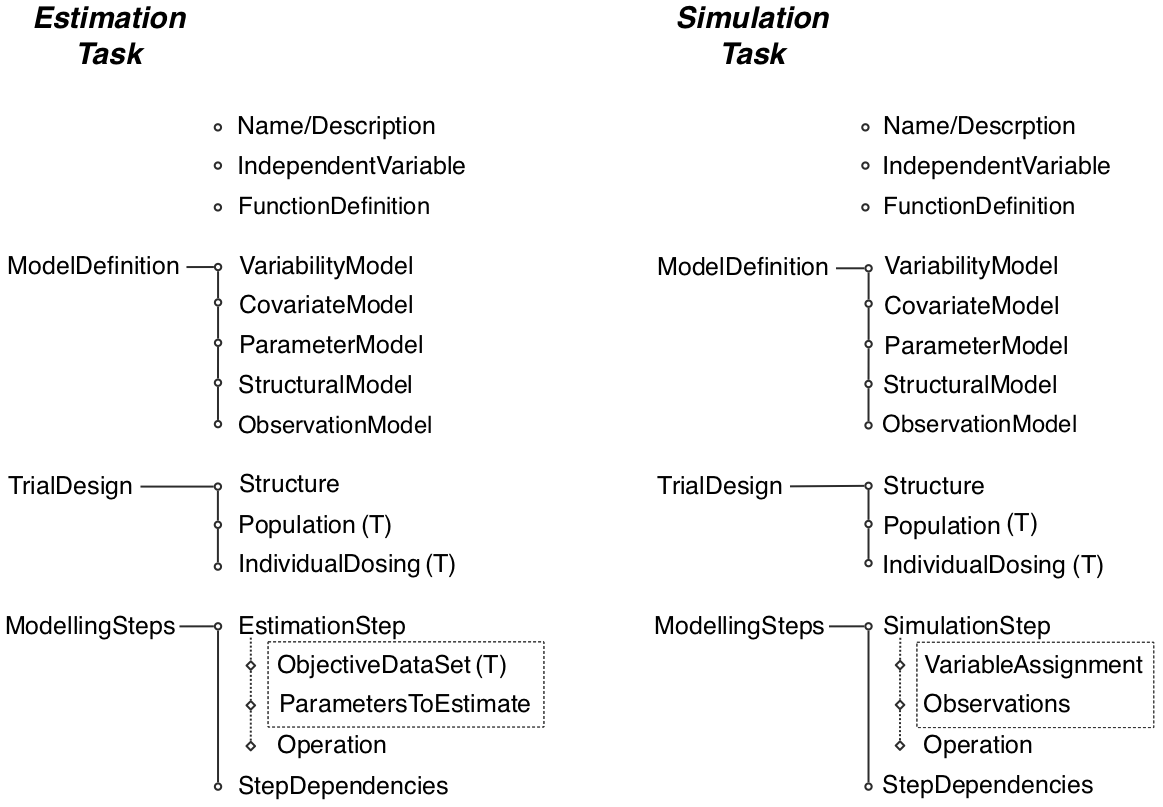
\includegraphics[width=0.8\linewidth]{pics/simEstTasks_List}%
 \caption{PharmML building blocks used in the trial definition for an estimation and simulation task. 
 Boxes underline elements where the structure of \pharmml for these two tasks differs. (T) indicates 
 that tabular data structure is used.}
 \label{fig:simEstTasks_List}
 \end{figure}

\eglabel{1}
\section{Example \theexamples: Simulation, PK + PD response}
\label{sec:eg1}

\subsection{Description}

%\subsubsection{Introduction}
\label{subsec:exp2_intro}

The following example is based on the CTS1 use case
\cite{Lavielle:2011}. Both PK (the drug concentration) and PD (the
drug effect) are simulated. A one compartment PK model is linked to an
indirect response PD model, see Figure \ref{fig:simplePKPD} for a typical 
simulation result for one patient.

\begin{figure}[ht!]
\begin{center}
\includegraphics[width=.45\textwidth]{pics/CTS1_smallPKPD}
\caption{Simulated combined model as defined in the example with PK (blue) and PD (green) time courses for one subject. Here three doses were administered every $48h$.}
\label{fig:simplePKPD}
\vspace{-20pt}
\end{center}
\end{figure}

\subsubsection{Model Definition}

\paragraph{Structural model}
This is an oral one compartment model and an indirect response model
with parameters \var{ka}, \var{V}, \var{CL}, \var{Imax}, \var{IC50},
\var{Rin} and \var{kout}.

\begin{align}
k&=\frac{\CL}{V}  \label{eqn:eg1-struct-model}\\
\frac{dAd}{dt} &=-ka \times Ad  \nonumber\\
\frac{dAc}{dt}&=ka \times Ad - k \times Ac  \nonumber\\
\frac{dE}{dt} &=Rin \times \Bigg(1-\frac{\Imax \times \Cc}{\Cc+\IC50}\Bigg)
- kout \times E \nonumber\\
\Cc &= \frac{Ac}{V} \nonumber
\intertext{initial conditions:}
E(t=0) &= \frac{Rin}{kout}  \label{eqn:eg1-init-conds}\\
Ad(t=0) &= 0  \nonumber\\
Ac(t=0) &= 0 \nonumber
\end{align}


\paragraph{Covariate model}

The only covariate is Weight, $W$, and it is a continuous covariate:
\begin{gather}
W \sim \mathcal{N}(\pop_{\Weight}, \omega_{\Weight}) \label{eqn:eg1-covariate-defn}
\intertext{The following transformation is applied:}
\log(\Weight/70) \label{eqn:eg1-covariate-trans}
\intertext{and the initial values are:}
\pop_{\Weight} =70.07, \quad \omega_{\Weight} =14.09 \nonumber
\end{gather}

\paragraph{Parameter model}

\subparagraph{PK parameters}

The model uses the following individual parameters:
\begin{description}
\item[\var{ka}] absorption rate constant
\item[\var{V}] volume of distribution
\item[\var{CL}] clearance of elimination
\end{description}
All follow a log-normal distribution:
\begin{align}
\log(ka_{i}) &=  \log(\pop_{ka}) + \eta_{ka,i}   \label{eqn:eg1-param-ka}\\
\log(V_i) &= \log(\pop_{V}) + \beta_{1,V}\log(W_i/70) + \eta_{V,i}   \label{eqn:eg1-param-V}\\
\log(\CL_i) &=  \log(\pop_{\CL}) + \beta_{1,\CL}\log(W_i/70) +
\eta_{\CL,i} \nonumber
\end{align}
where
\begin{gather*}
\eta_{ka,i} \sim N(0, \omega_{ka}), \quad \eta_{V,i} \sim N(0,
\omega_{V}), \quad \eta_{\CL,i} \sim N(0, \omega_{\CL})
\intertext{with initial values:}
\pop_{ka}=1,\quad \omega_{ka}=0.6  \qquad \pop_V=8,\quad \omega_V=0.2 \\
\pop_{\CL}=0.13,\quad \omega_{\CL}=0.2  \qquad \beta_{1,V}=1 , \quad \beta_{1,\CL}=0.75  \\
\rho_{V,\CL}=0.7\footnotemark
\end{gather*}
\footnotetext{Correration coefficient between $\eta_{V,i}$ and $\eta_{\CL,i}$}

\subparagraph{PD parameters}

The model uses the following individual parameters:
\begin{description}
\item[\var{Imax}] maximal antagonistic response
\item[\var{IC50}] concentration giving half the maximal response
\item[\var{Rin}] input (synthesis) rate
\item[\var{kout}] output (elimination) rate
\end{description}
All follow a log-normal distribution, except \var{Imax}, which follows a logit-normal distribution.
\begin{align*}
\logit(Imax_i) =& \logit(\pop_{Imax})  + \eta_{Imax,i}   \\
\log(\IC50_{i}) =& \log(\pop_{\IC50}) + \eta_{\IC50,i}  \\
\log(\Rin_i) =& \log(\pop_{\Rin}) + \eta_{\Rin,i}  \\
\log(\kout_i) =& \log(\pop_{\kout}) + \eta_{\kout,i}
\end{align*}
where
\begin{gather*}
  \eta_{Imax,i} \sim N(0, \omega_{Imax}), \quad \eta_{\IC50,i} \sim
  N(0, \omega_{\IC50}), \\
\eta_{\Rin,i} \sim N(0, \omega_{\Rin}), \quad \eta_{\kout,i} \sim N(0, \omega_{\kout})
\intertext{with initial values:}
\pop_{Imax} =0.9,\quad \omega_{Imax}=2  \qquad \pop_{\IC50} =
0.4,\quad \omega_{\IC50} =0.4  \\
\pop_{\Rin}=5, \quad \omega_{\Rin}=0.05  \qquad \pop_{\kout} =0.05,
\quad \omega_{\kout} =0.05
\end{gather*}

\paragraph{Variance-covariance matrix}
\label{sec:covariance-matrix}
The full variance-covariance matrix for the random effects is:
\begin{gather}
 \Omega =
 \begin{pmatrix}
  \omega_{ka}^2 	& 0 				& 0  				& 0  				& 0  				& 0  				& 0  				\\
   			  	& \omega_{V}^2	& \omega_{V,\CL} 	& 0  				& 0  				& 0  				& 0  				\\
  				& 				& \omega_{\CL}^2	& 0  				& 0  				& 0  				& 0  				\\
 				&				&   				& \omega_{Imax}^2  & 0  				& 0  				& 0  				\\
				&   				&   				&   				& \omega_{IC50}^2  & 0  				& 0  				\\
				&   				&   				&   				&   				& \omega_{Rin}^2 	& 0  				\\
				&   				&   				&   				&   				&   				& \omega_{kout}^2
 \end{pmatrix}
\intertext{where}
\omega_{V,\CL} = \omega_\var{V} \, \omega_{\CL} \,\rho_{\var{V},\CL}\nonumber
\label{sec:eg-covariance-mat}
\end{gather}

\paragraph{Observation model}
\label{sec:eg1-desc-obs-model}

We apply a residual error model to the output variables \var{Cc} and \var{E}
from the PK and PD models respectively.

%\begin{table*}[h!]
\begin{center}
\begin{tabular*}{0.8\linewidth}{@{\extracolsep{\fill}} >{\bfseries}l l l}\toprule
Output Variable & \textbf{\itshape Cc} &\textbf{\itshape E}\\\midrule
Observation Name & Concentration & PCA\\
Units & $\mg/l$ & $\%$\\
Type & Continuous & Continuous \\
Model & Combined & Constant \\
Parameters & $a = 0.5,\quad b=0.1$ & $a=4$\\
\bottomrule
\end{tabular*}
\end{center}

%%%%%%%%%%%%%%%%%%%%%%%%%%%%%%%%%%%%%%%%%%%%%%%%%%%%%%%%%%%%%%%%
\subsubsection{Trial Design}
\label{subsec:exp2_TaskDescription}

\begin{figure}[h!]
\centering
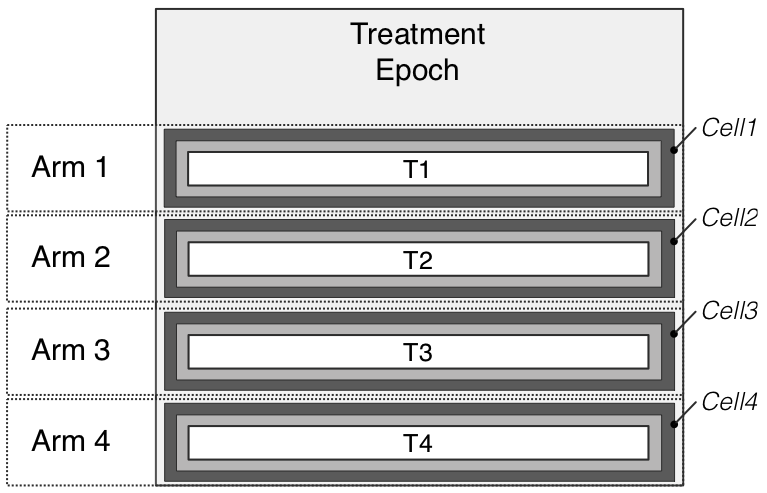
\includegraphics[width=0.7\linewidth]{../pics/designPattern_4Arms1Epoch}
\caption{Design overview: this study consists of four arms and one epoch. The differences between arms lie in the number of subjects, dose amount and times. See table below for the details.}
\label{fig:designPattern_4Arms1Epoch}
\end{figure}

Figure \ref{fig:designPattern_4Arms1Epoch} shows the \textit{Structure} of
this example consisting of four arms and one epoch, meaning there are four treatment
types for which only one time period needs to be specified.

The dosing regimen for the trial is given for each arm below. Note
that all dosing is bolus dosing (discrete administration at specific
times) and all doses are administered to the same compartment.

%\begin{table*}[h!]
\begin{center}
\begin{tabular*}{0.9\linewidth}{@{\extracolsep{\fill}} >{\bfseries}l rrrr}\toprule
Arm & \textbf{1} &\textbf{2} &\textbf{3} & \textbf{4}\\\midrule
Number of subjects & 20 & 20 & 40 & 40 \\
Dose target & \var{Ad} & \var{Ad} & \var{Ad} & \var{Ad}\\
Dosing Amount & 0.25 & 0.5 & 0.5 & 1\\
Dose Units & $\mg/\kg$  & $\mg/\kg$  & $\mg/\kg$  & $\mg/\kg$ \\
Dose per kg & yes & yes & yes & yes\\
Dosing times (h) & 0:24:192 &  0:48:192 &  0:24:192 & 0:48:192 \\
\bottomrule
\end{tabular*}
\end{center}


%%%%%%%%%%%%%%%%%%%%%%%%%%%%%%%%%%%%%%%%%%%%%%%%%%%%%%%%%%%%%%%%
\subsubsection{Modelling Steps}

Time of measurement for PK and PD happens according to different
schedules and these observation time points are produced by the
simulation. The output variables to be generated by the simulation and
their associated time points are shown below:

\begin{center}
\begin{tabular*}{0.9\linewidth}{@{\extracolsep{\fill}} >{\bfseries}l c c}\toprule
Output Variable & \textbf{\itshape Cc} &\textbf{\itshape E}\\\midrule
Observation times & [0.5,4 : 4 : 48,52 : 24 : 192,192 : 4 : 250] & 0 : 24 : 288\\
\bottomrule
\end{tabular*}
\end{center}

%%%%%%%%%%%%%%%%%%%%%%%%%%%%%%%%%%%%%%%%%%%%%%%%%%%%%%%%%%%%%%%%
\subsection{\pharmml Document Structure}
\label{sec:symbol-defn}
An overview of the model with the key sections collapsed  as shown in this listing
\inputxml{exp1_lst1.xml}
illustrates the main sections of the model as described
in section \ref{sec:structure-overview}. The key points to note are
the use of the \xatt{independentVar\-iable}  attribute to set the time
variable to $t$ (c.f.\xspace section \ref{sec:independent-var}), and
how the element \texttt{Name} defines the name of the model. In addition
the top-level \texttt{PharmML} element contains a number of attributes
prefixed \texttt{xmlns}. These are required by the XML Schema standard
and can be ignored as we go through the examples\footnote{If you
  want to learn more about the technical aspects of XML and the XML Schema standard
  used to define \pharmml then we recommend to start here:
  \url{http://www.w3.org/TR/xmlschema-0/}. And, by the way,
  \texttt{xmlns} stands for XML namespace.}.

%\begin{listing}[htb]
%\inputxml{exp1_lst1.xml}
%\caption{An overview of the \pharmml document for example \egref{1}.}
%\label{eg:eg1-overview}
%\end{listing}

The above listing introduces a concept and XML element that we did not describe
before: this is the \xelem{FunctionDefinition} element. It defines a function that
returns a real type as shown in the following listing 
%\ref{eg:symboldefn}. 
\inputxml{exp1_lst2.xml}

The function takes three arguments of scalar type and defines the
function:
\begin{displaymath}
\var{combinedError}(a, b, f) = a + bf
\end{displaymath}
This function is used to encode the combined error model function used later in
the observation model (see section \ref{sec:eg1-obs-model}).

%\begin{listing}[htb]
%\inputxml{exp1_lst2.xml}
%\caption{Function definition using the \xelem{FunctionDefinition} element.}
%\label{eg:symboldefn}
%\end{listing}

%%%%%%%%%%%%%%%%%%%%%%%%%%%%%%%%%%%%%%%%%%%%%%%%%%%%%%%%%%%%%%%%%
%\subsubsection{Units}
%\label{sec:eg1-units}
%
%Listing \ref{eg:eg1-units} shows how we define units for this example, see for details \ref{sec:units}. It is done using the element \xelem{UnitDefinition} and child element \xelem{UnitComponent}. For example $mg$ for tumour mass or $mg/kg$ as dose unit to express the dosing per kilogram of body weight.
%
%\begin{listing}[htb]
%\inputxml{exp1_units.xml}
%\caption{Examples of the units definition in example \egref{1}.}
%\label{eg:eg1-units}
%\end{listing}
%


%%%%%%%%%%%%%%%%%%%%%%%%%%%%%%%%%%%%%%%%%%%%%%%%%%%%%%%%%%%%%%%%
\subsection{Model Definition}

As you can see in the following listing 
\inputxml{exp1_lst3.xml}

the model definition section defines the main components that you will see in
the subsequent examples. Apart from the structural model, all of these
elements are optional and all follow the scoping rules described in
section \ref{sec:blocks}.

%\begin{listing}[htb]
%\inputxml{exp1_lst3.xml}
%\caption{Overview of the Model Definition section in example \egref{1}.}
%\label{eg:eg1-modeldefn-overview}
%\end{listing}

%\begin{listing}[htb]
%\inputxml{exp1_lst3A.xml}
%\caption{In example \egref{1} there are two variability models, one related
%to the IIV and one related to the residual error.}
%\label{eg:eg1-residualAndIndividual}
%\end{listing}


%%%%%%%%%%%%%%%%%%%%%%%%%%%%%%%%%%%%%%%%%%%%%%%%%%%%%%%%%%%%%%%%
\subsubsection{Variability Model}
\label{sec:eg1-variability}

\begin{figure}[ht!]
\centering
 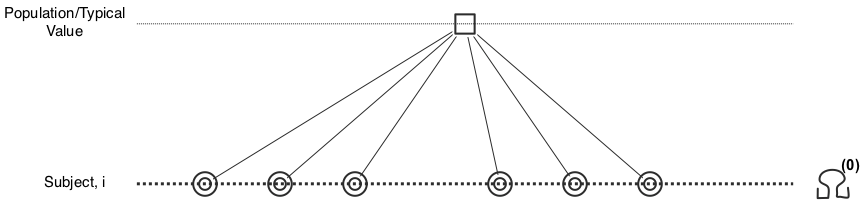
\includegraphics[width=120mm]{tree_IOV0}
\caption{There is only one level of variability in this example -- inter-individual variability.}
\label{fig:tree_IOV0}
\end{figure}

From the listing above one can also see that there
are two variability models defined using the element
\xelem{Vari\-abilityModel}. This is how we explicitly define the
level of variability in the model (c.f.\ section
\ref{sec:variabilityModel}). In this case there is one level of 
variability, the inter-individual, Figure \ref{fig:tree_IOV0} and the residual
error model variability, see the following listing \inputxml{exp1_lst3A.xml}
for the details of the implementation. Please, note that we use two different variability 
attribute types, \xatt{model} and \xatt{error}. The former stands for random variability
associated with the parameters, as described in section \ref{sec:variabilityModel}. 
For this example we are defining one level of variability in the parameter model and this
corresponds to variability between subjects. The latter stands for residual error variability.

We will explain this more fully below when we look at
examples with more complex variability models (section
\ref{eg6:variabilityModel}).

%%%%%%%%%%%%%%%%%%%%%%%%%%%%%%%%%%%%%%%%%%%%%%%%%%%%%%%%%%%%%%%%
\subsubsection{Covariate Model}
\label{sec:eg1-covariate}


The \xelem{CovariateModel} block corresponds to the covariate model
defined in section \ref{maths:covariate_model}. In this example, as shown
in this listing \inputxml{exp1_lst4and5.xml}
we are defining a continuous
covariate, \var{W}, indicated by the \xelem{Continuous} element and
the covariate is sampled from a normal distribution as in equation
\ref{eqn:eg1-covariate-defn}.  The element \xelem{Transformation}
beneath the definition of the distribution describes the
transformation applied to this covariate whenever it is used. In this
case the transformation being applied is defined in
equation~\ref{eqn:eg1-covariate-trans}.

%\begin{listing}[htb]
%\inputxml{exp1_lst4and5.xml}
%\caption{The Covariate Model}
%\label{eg:eg1-covariate-model}
%\end{listing}



%%%%%%%%%%%%%%%%%%%%%%%%%%%%%%%%%%%%%%%%%%%%%%%%%%%%%%%%%%%%%%%%
\subsubsection{Parameter Model}
\label{sec:eg1-pk}
All parameters in the current example \egref{1} can be defined
using the Gaussian model with linear covariates (see section
\ref{sec:parameterModel}). We will start with a simple case in this
example, shown in the following listing \inputxml{exp1_lst6.xml}
the absorption rate constant \var{ka}. 
First the typical value for \var{ka}, \var{pop\_ka}
and the standard deviation of the random effect, \var{\omega\_ka}, are
defined as \xelem{SimpleParameter}'s. Then the random effect \var{eta\_ka}
is defined, and it follows a normal distribution with mean $0$ and
standard deviation \var{\omega\_ka}.

Then the actual individual parameter \var{ka} is
defined with the \xelem{Transformation} attribute set to
\texttt{log}. This tells us that the parameter is log-transformed. We
are using the Gaussian model described previously (section
\ref{maths:parameter-model}), and it follows a log-normal distribution
with the mean \var{pop\_ka} and the standard deviation
 \var{omega\_ka}, as shown in equation \ref{eqn:eg1-param-ka}.
Even though \var{ka} is modelled without a covariate, we still use the
element \xelem{LinearCovariate}, which contains here logically only the
typical value element \xelem{PopulationParameter}.

%\begin{listing}[htb]
%\inputxml{exp1_lst6.xml}
%\caption{A simple parameter definition: parameter $ka$.}
%\label{eg:eg1-param-prt1}
%\end{listing}

The \xelem{RandomVariable} element is very important here. It tells us
what the random effect is, and, by assigning a variability level to
the attribute \xatt{symbIdRef} within the \xelem{VariabilityRef\-erence} element,
it effectively tells us that the random effect is sampled for every subject.
The importance of this will become clearer in later examples that describe
multiple levels of variability. Note that the \xelem{RandomVariable} element
also defines a new symbol \var{eta\_ka}, which is a parameter.


%\begin{listing}[htb]
%\inputxml{exp1_lst7.xml}
%\caption{A more complicated parameter definition: parameter $V$.}
%\label{eg:eg1-param-prt2}
%\end{listing}

Of course not all parameter definitions are so straight forward. In the
following listing \inputxml{exp1_lst7.xml}
you can see the definition of a
parameter, \var{V}, that is related to the covariate, $W$. We do this
using the element \xelem{Covariate} to indicate there is a
relationship. Then we reference the specific covariate (using the
\xelem{SymbRef} element) and describe the fixed effect relating the
covariate to this parameter: in this case we are referring to the
parameter \var{beta\_V}. We define here a linear covariate model
when relating covariates to parameters (c.f.\xspace section
\ref{maths:covariate_model}), so this example corresponds to
equation \ref{eqn:eg1-param-V}.

You may have noticed that in equation \ref{eqn:eg1-param-V} the
covariate term is $\log\left(W/70\right)$ and not \var{W}. Why? Well
we have applied the covariate transformation defined in
(\ref{eqn:eg1-covariate-trans}). As we described above (section
\ref{sec:eg1-covariate}), whenever a covariate is used here we always
apply any transformation defined in the \xelem{Transformation}
element.

Having defined the individual and other parameters in the parameter
model we need to describe the correlation of the random effects, if any.
As described above (see section \ref{subsec:correlationModel} for
a complete description) we do this using a covariance matrix.
In \pharmml, if the random effects of both
parameters follow a normal distribution, then we assume that the
diagonal of the covariance matrix can be derived from the variance or
standard deviation of each parameter (c.f section
\ref{maths:covariance-mat-derivation}). This is true in our example,
so we only need to define the parts of the covariance matrix that
define the correlation between parameters \var{V} and \var{CL}
as shown in this listing \inputxml{exp1_lst8.xml}
Notice that with the
\xatt{symbIdRef} attribute the correlation is associated with the
variability level defined at the beginning of the model
definition. This allows us to define a covariance matrix for each
level of variability in the model and thus to define different
parameter correlations at each level as well. This single
\xelem{Correlation} element is all we need to define the covariance
matrix mentioned above (section \ref{sec:eg-covariance-mat}).

%\begin{listing}[htb]
%\inputxml{exp1_lst8.xml}
%\caption{The correlation of parameters \var{V} and \var{CL}.}
%\label{eg:eg1-param-prt3}
%\end{listing}

You now know most of the structures used to define a parameter in
\pharmml. As you will see later, these elements can be combined to
create more complicated parameter models, but these are elaborations
of this framework.

%%%%%%%%%%%%%%%%%%%%%%%%%%%%%%%%%%%%%%%%%%%%%%%%%%%%%%%%%%%%%%%%
\subsubsection{Structural Model}

In \pharmml the structural model can be described using algebraic
equations or an ODE system. In this example the
model is defined as a combination of an ODE system and
some supporting algebraic equations (c.f.\xspace equation \ref{eqn:eg1-struct-model}).

%\begin{listing}[htb]
%\inputxml{exp1_lst9and10.xml}
%\caption{A subset of the structural model showing how variables
%  \var{k} and \var{Ad} are defined and how we specify the initial condition for a
%  variable defined by an ODE.}
%\label{eg:eg1-struct-prt1}
%\end{listing}

The following listing \inputxml{exp1_lst9and10.xml} illustrates how the variable \var{k}
is defined. We cover this in more detail in chapter
\ref{chap:lang-overview}, but briefly: \var{k} is defined as having a
real type and is assigned the result of the expression $CL/V$, which
are parameters defined in the parameter model, \var{p1}. We can also
see how the derivative \var{Ad} is defined using the element \xelem{DerivativeVariable}
(see section \ref{sec:odes} for a more detailed explanation)
with $t$ as the independent variable. The full ODE defined is:
\[
\frac{\mathrm{d}\,\var{Ad}}{\mathrm{d}t} = -\var{ka} \, \var{Ad}
\]
where \var{ka} is a parameter defined in the parameter model \var{p1}.
Finally the \xelem{InitialCondition} element defines
the initial value for \var{Ad} at time 0, here $Ad(t\!=\!0)\!=\!0$, which is the default initial time
in \pharmml.
%\begin{listing}[htb]
%\inputxml{eg1_struct_model_prt2.xml}
%\caption{Defining the initial conditions of the model.}
%\label{eg:eg1-struct-prt2}
%\end{listing}
%
%Since this defines a system of differential equations, we need to
%define the initial conditions. Second part of listing \ref{eg:eg1-struct-prt1} shows
%how the initial conditions in equation \ref{eqn:eg1-init-conds} are defined
%in \pharmml. Very simply the result of a mathematical expression described in
%\pharmml Maths is assigned to the variables at $t=0$.

%%%%%%%%%%%%%%%%%%%%%%%%%%%%%%%%%%%%%%%%%%%%%%%%%%%%%%%%%%%%%%%%
\subsubsection{Observation Model}
\label{sec:eg1-obs-model}

In this example there are two observations for the continuous
variables \var{Cc} and \var{E}, which are outputs from the structural
model. As described above each has a residual error model applied to it.

%\begin{listing}[htb]
%\inputxml{exp1_lst11.xml}
%\caption{The residual error model applied to variable \var{Cc}.}
%\label{eg:eg1-obs}
%\end{listing}

The XML is very similar for both variables so in the following listing 
%\ref{eg:eg1-obs} 
\inputxml{exp1_lst11.xml}
we only show how the residual error model for \var{Cc}, the continuous PK variable, is defined.
First the parameters of the residual error model \var{a} and \var{b} are
defined using \xelem{SimpleParameter}; here a combined additive
and proportional error model is applied. Then \var{epsilon\_Cc} as \xelem{RandomVariable}
of the residual error model with a mean of $0$ and standard deviation \var{sigma\_Cc} is defined
to be used in the subsequent parts of the model. Note that we need to 
indicate the type and level of the according random effect which were
defined in the 'Variability Model' section above. This is done
using the \xelem{VariabilityReference} 

The subsequent element \xelem{Standard} states that we are defining a standard
continuous observation model. This means in short that we can define
an observation model of the form $y_{ij} = f_{ij} + g\times\epsilon_{ij}$
(for details, see the discussion below and section \ref{sec:observationModel}).

The attribute \xatt{symbId} of \xelem{Standard} defines the name of the
variable that will hold the result of the applied residual error model.
The \xelem{Output} element then defines the
variable in the structural model that the residual error model applies to
(in this case \var{Cc}). Next we define the actual residual error
model with the \xelem{ErrorModel} element. The error model is invoked
by calling the function \var{combinedErrorModel} defined in the symbol
definition at the beginning of the \pharmml document (see section
\ref{sec:symbol-defn}). We pass in the appropriate parameter values
(see section \ref{maths:combined-err-model} for a description of the
residual error model) and this defines our residual error model.\\
Finally we use the \xelem{ResidualError} element to reference the
\var{epsilon\_Cc} specified before.



%%%%%%%%%%%%%%%%%%%%%%%%%%%%%%%%%%%%%%%%%%%%%%%%%%%%%%%%%%%%%%%%%%
\paragraph{Residual model implementation}
Most residual error model types have two or three equivalent forms, by which 
we mean they have the same variance, although they use one or more residual 
errors, $\epsilon_{ij}$, see examples in section \ref{subsec:modelExamples}. 
Other types contain two or more predictions from the structural model, \var{f_{ij}}. 
From a computational point of view it makes a lot of sense to reflect such 
differences in the language structure.
This was the motivation to allow for the implementation of two types of observation models
\begin{itemize}
\item
\xelem{Standard} -- any observation model of the form
\begin{align*}
	u(y_{ij}) = u(f_{ij}) + g\times\epsilon_{ij}
\end{align*}
which can be defined using exactly one of the following items
\begin{itemize}
\item
a transformation, $u$, e.g. \var{log} or \var{logit}
\item
one structural model prediction, \var{f_{ij}}
\item
one standard deviation function, \var{g}
\item
one random variable, $\epsilon_{ij}$
\end{itemize}
\item
\xelem{General} -- using any number of the items listed above and arbitrary functional relationship between them.
\end{itemize}
This chapter contains more examples illustrating these constructs.

%We described in chapter \ref{chap:mathsdefn} (section
%\ref{sec:residualErrorModel}) how we currently assume the residual
%error model to be of the form $g\epsilon$, where $g$ is the error
%model and $\epsilon$ is a random value sampled from a probability
%distribution. In \pharmml (listing \ref{eg:eg1-obs}) the
%\xelem{RandomEffect} element defines $\epsilon$. This element is
%similar to its namesake in the parameter model in that it describes a
%probability distribution, but in this case it is not associated with a
%level of variability nor do we assign it symbol name. In the listing
%the distribution was omitted to save space, but it is defined in
%exactly the same way as it is in the parameter model.

%%%%%%%%%%%%%%%%%%%%%%%%%%%%%%%%%%%%%%%%%%%%%%%%%%%%%%%%%%%%%%%%
\subsection{Trial Design}
\subsubsection{Structure}

In this fairly simple case, there is only one epoch and four arms, \var{Arm\_1}, \var{Arm\_2} etc.,
cf. Figure \ref{fig:designPattern_4Arms1Epoch}.
The resulting four cells \var{Cell\_1}, \var{Cell\_2} etc. each correspond
to one arm and contain one segment.
Figure \ref{fig:CellSegmentEpochArm_example1} (right) illustrates the inter-relationship between
cells, arms, epochs and segments. Here a segment consists of one activity --
a certain type of treatment. In general, a segment can contain more
than one activity. Dosing regimen can be defined for different
compartments in the structural model. In this example there are four
treatments with one dosing regimen per treatment.

\begin{figure}[htbp!]
\centering
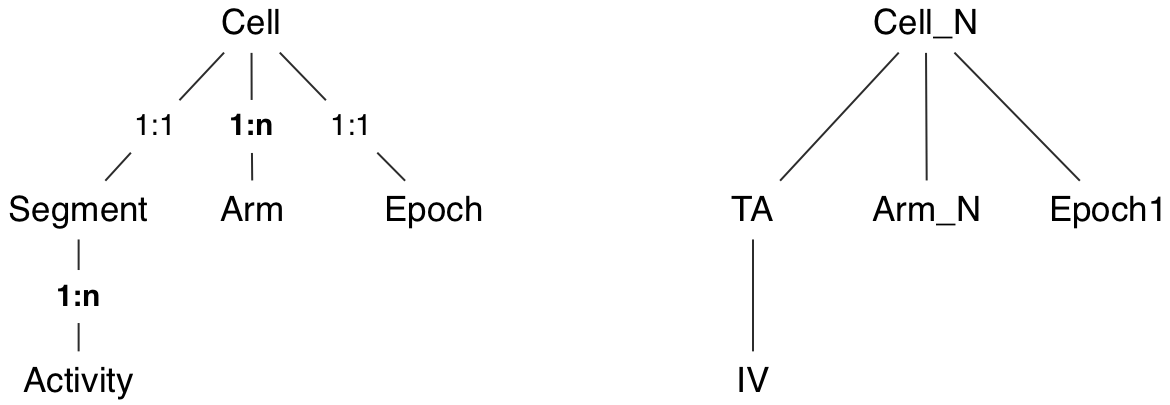
\includegraphics[width=0.7\linewidth]{pics/CellSegmentEpochArm_example1}
\caption{(left) General cell hierarchy; (right) How it is applied in example \egref{1}.
There is only one epoch and four arms, \var{Arm\_1}, \var{Arm\_2} etc.
The resulting four cells \var{Cell\_1}, \var{Cell\_2}, etc. each correspond
to one arm and contain one segment. See the listing bellow for how
these features are implemented and structured.}
\label{fig:CellSegmentEpochArm_example1}
\end{figure}

%The treatment in \pharmml is used to describe the dosing regimen
%applied to the subjects in the trial. A treatment can contain more
%than one dosing regimen and drugs can be administered to different
%compartments in the structural model. In this example there are four
%treatments with one dosing regimen per treatment.

%\begin{listing}[htb]
%\inputxml{exp1_lst12.xml}
%\caption{A treatment with bolus dosing.}
%\label{eg:eg1-treatment}
%\end{listing}

%\ref{eg:eg1-treatment} 
In the following listing 
\inputxml{exp1_lst12.xml} we show an activity defined for \var{Arm\_1},
here treatment in the form of a bolus administration: the others are very similar.
The \xelem{Activity} element is given an identifier, ``\texttt{d1}'',
and the element \xelem{Bolus} defines a
bolus administration\footnote{Bolus and infusion are the only types of
dosing regimen permitted. We make no distinction between oral and IV
administration as such differences are handled by the structural
model used.}.  \xelem{DoseAmount} defines the amount of drug to be
administered. The are basically two options here. Either the dose is assigned
to the variable defined by an ODE, such is the case here, for which we use
\xatt{inputType="target"} attribute or the dosing variable \var{D} as in algebraic
equations. 
Additionally, in this case the administration is adjusted for body
weight using the expression $0.25W$. The element \xelem{SymbIdRef}
defines the target of dosing. This effectively defines an input
function that adds the dose amount
to the variable \var{Ad} at the specified dosing time. The dosing
times themselves are given by the \xelem{DosingTimes} element as the
sequence $0:24:192$.
% (see section \ref{sec:arrays} for more information about sequences).

%%%%%%%%%%%%%%%%%%%%%%%%%%%%%%%%%%%%%%%%%%%%%%%%%%%%%%%%%%%%%%%%%
%\subsubsection{Treatment Epoch and Group}

%In this example (listing \ref{exp1_lst13}) the purpose of the
%Treatment Epoch is not clear. In general the treatment epoch provides
%a time-frame that dosing times are relative to, and this permits us to
%define more complex trial design structures as you will see in later
%examples. However, in this simple example no time-frame is defined so
%it is assumed to be the interval $[0, \inf]$ (see section
%\ref{maths:epoch-defn}). The epoch can contain one or more treatments,
%which are referenced using the \xelem{TreatmentRef} element.

%\begin{listing}[htb]
%\inputxml{exp1_lst13.xml}
%\caption{Arm, cell, epoch and segment/activity definition (see Figure
%\ref{fig:CellSegmentEpochArm_example1} for the relationship between
%these elements).}
%\label{exp1_lst13}
%\end{listing}

Once the segments with their according treatments/activities are defined, we can define epochs using the
element \xelem{Epoch} with their start and stopping time along with their order.
After the arms are specified, the \xelem{Cell} element is used to put all of the components together, see this listing 
\inputxml{exp1_lst13.xml}

%%%%%%%%%%%%%%%%%%%%%%%%%%%%%%%%%%%%%%%%%%%%%%%%%%%%%%%%%%%%%%%%
\subsubsection{Population}

The \xelem{Population} is the second and in the case of a simulation example,
also the last block in the trial design definition. As explained in chapter \ref{sec:CTS}
this is the place to define the number of subjects per study arm, constant
or time-varying covariates and other properties, if available.
In this particular case covariates are simulated according to 
the definition in eq.\ref{eqn:eg1-covariate-defn}. This is the reason the following table with 
population data will have only three columns. (In case of estimation the covariates would have to 
be listed explicitly in this table as well, this will be described in the next example \ref{sec:eg4})\\
The definition of the table is in the \xelem{IndividualTemplate} block where the columns
\var{id}, \var{arm} and \var{reps} are specified, see the following listing 
\inputxml{exp1_lst13A.xml}
Using the \var{reps} variable allows us
to shorten the definition in cases where all other features are the same across subjects in
an arm, which is the case here. Here four arms with 20, 20, 40 and 40 subjects, respectively, are defined.
An alternative would be to list all subjects explicitly, in which case only two columns would be
sufficient, \var{id} and \var{arm}.\\
In the estimation case another block \xelem{IndividualDosing} would have to be defined as next.
This will be explained in the following example \ref{sec:eg4}.

%The trial group, defined by the \xelem{Group} element, brings together
%the epochs (referred to by the \xelem{TreatmentEpochRef} element) and the
%individuals (or subjects) in the trial. We define the number of
%individuals in the trial using the \xelem{Individuals} element and we
%also assign them a variable, \var{i}. This variable can be used to refer
%to the individuals within this group (see example \egref{5} in section
%\ref{sec:eg4}) and will also be useful when \pharmml is extended
%to describe the export of results to a file. Note that for the purposes
%of variable scoping the \xelem{Group} element defines a block and so
%this variable must be referred to as: \verb|<math:Var block="a1" symbId="i"/>|


%\begin{listing}[htb]
%\inputxml{exp1_lst13A.xml}
%\caption{Population definition.}
%\label{eg:eg1-population}
%\end{listing}


%%%%%%%%%%%%%%%%%%%%%%%%%%%%%%%%%%%%%%%%%%%%%%%%%%%%%%%%%%%%%%%%
\subsection{Modelling Steps}
\label{sec:eg1-modelingSteps}

\subsubsection{Simulation settings and dependencies}

In the following listing \inputxml{exp1_lst14.xml}
you can see the structure of the
\xelem{ModellingSteps} section of \pharmml.  In this example we are
describing a simulated model and so use the \xelem{SimulationStep}
element.

%The step is given an ``\texttt{oid}'' identifier, ``\texttt{s1}'', and then we
%specify the number of times the simulation is to be executed (number
%of replicates) using the \xelem{Replicates} element. A variable name
%is defined here (of scalar type), in this case \var{r}, that is holds
%the number of the current replicate. This variable is not currently
%used by the rest of the simulation, block, but the intention is that
%it will become useful in the future when describing the export of
%results within \pharmml. In the meantime this variable is likely to be
%useful for software tools as it gives a recognisable variable name to
%describe the replicates in an implementation based on this \pharmml
%document.

%\begin{listing}[htb]
%\inputxml{exp1_lst14.xml}
%\caption{Simulations steps in outline.}
%\label{eg:eg1-ms-deps}
%\end{listing}

The first part of the simulation block sets initial values for
parameters in the model and defines the outputs of the simulation. We
will go into more detail on these elements below. Then at the end of
the modelling steps block is the \xelem{StepDependencies}
element. This describes the ordering of the steps in the modelling
steps section (see section \ref{sec:stepdeps}), but in this case it is
redundant as we only have one step in this example.

\subsubsection{Initial Values}

The code snippet in listing \inputxml{exp1_lst15.xml}
shows how we set
initial values. Very simply we refer to a previously defined variable,
here the typical value for a covariate \var{pop\_W}, or parameter and then assign
it a numerical value within the \xelem{VariableAssignment} element.
In this example the value for \var{omega_W} is
calculated from a mathematical expression, which is allowed, if this expression
resolves to a numerical value.  The order of the \xelem{VariableAssignment}
elements is not significant and the ordering is based on variable
dependencies (as described in section \ref{sec:symbolScoping} on page
\pageref{sec:symbolScoping}).

%\begin{listing}[htb]
%\inputxml{exp1_lst15.xml}
%\caption{Assigning initial values in the simulation step.}
%\label{eg:eg1-ms-init-vals}
%\end{listing}

\subsubsection{Observations}

Typically, what drives a simulation task are its outputs. You only
need to simulate the parts of your system that produce the required
outputs and for as long as you wish to observe those outputs. In
\pharmml we use the \xelem{Observations} element to do this job, as
you can see in this listing \inputxml{exp1_lst16.xml}
In this example we define
a set of time points, $0.5, 4:4:48, 52:24:192, 192:4:250$, and the
variables we would like to see simulated at those points in time. You
can define one or more output variables here using the \xelem{Continuous}
element. It is noteworthy here that by choosing the \var{Cc} defined
in both the structural model (``\texttt{main}'') and observation
model (``\texttt{o1}'') blocks we can show the output of the
structural model with and without the residual error applied.

%\begin{listing}[htb]
%\inputxml{exp1_lst16.xml}
%\caption{Defining output observations of the simulation.}
%\label{eg:eg1-ms-obs}
%\end{listing}

%\clearpage
%%\newpage


% BONATE
%%%%%%%%%%%%%%%%%%%%%%%%%%%%%%%%%%%%%%%%%%%%%%%%%%%%%%%%%%%%%%%%
%%%%%%%%%%%%%%%%%%%%%%%%%%%%%%%%%%%%%%%%%%%%%%%%%%%%%%%%%%%%%%%%
%%%%%%%%%%%%%%%%%%%%%%%%%%%%%%%%%%%%%%%%%%%%%%%%%%%%%%%%%%%%%%%%
\eglabel{2}
\section{Example \theexamples: Simulation with steady state dosing}
\label{sec:eg2}

\subsection{Description}

The following example is taken from \cite{Bonate:2011fk}, p.535, and represents another simple example for a PK simulation. However, here we discuss a system under steady state resulting from a twice daily dosing in 50 adult subjects who received a dose of 100 mg per administration. The drug concentration follows a 1-comp model with first order absorption with a proportional residual error model.
\begin{figure}[ht!]
\begin{center}
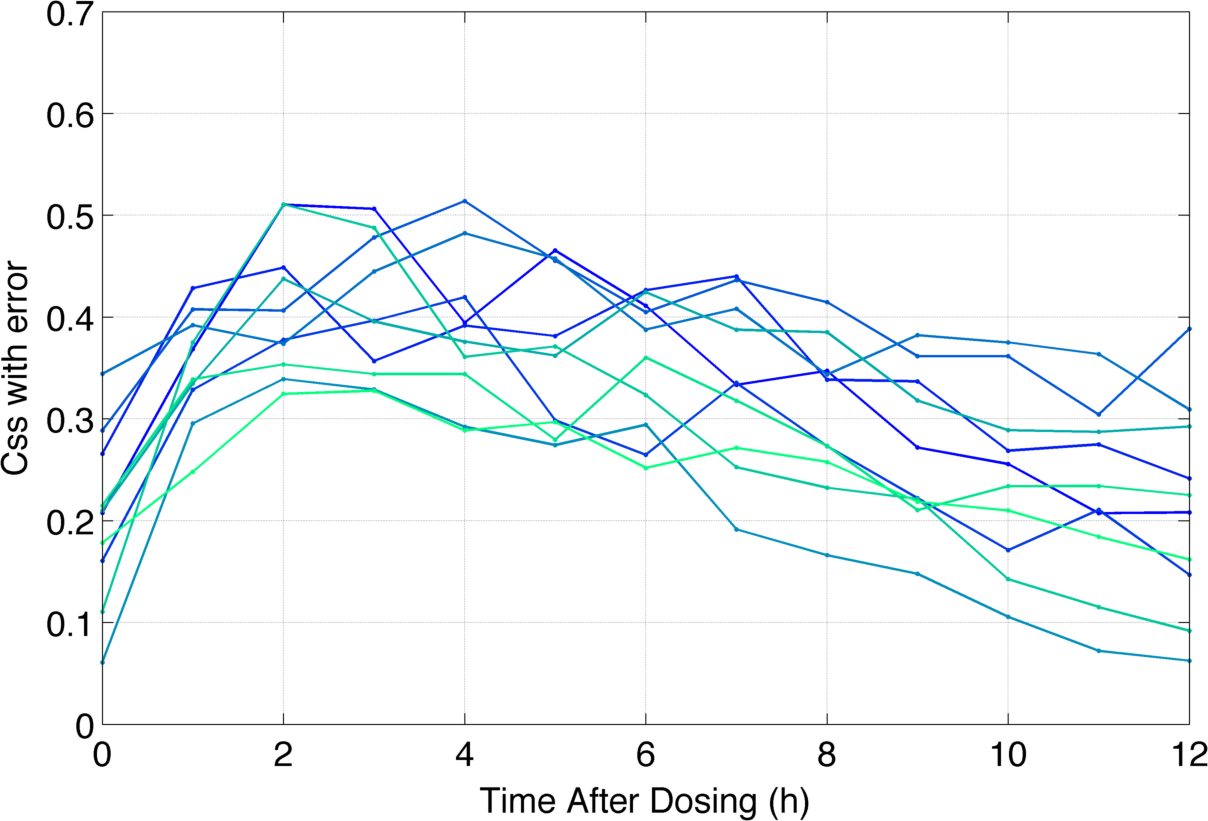
\includegraphics[width=.45\textwidth]{pics/Bonate_Css_proportionalError}
\caption{Simulated PK model as defined in the example for 10 subjects.}
\label{fig:BonatePK}
\vspace{-20pt}
\end{center}
\end{figure}
The only essential new aspect compared to the previous example is the fact
that we have here so called steady-state administration. For this to be defined
one needs to provide the time point of the last dosing event and the dose interval.

\subsubsection{Variability model}
The variability structure is identical to that in the previous example -- there is only
one level of subject related variability, see Figure \ref{fig:tree_IOV0}.

\subsubsection{Parameter model}

The model uses the following parameters:

\begin{align*}
\theta_{1,i} &=  \pop_{\theta_1} + \eta_{\theta_1,i}   \\
\log(V_i) &= \log(\pop_{V}) + \eta_{V,i}   \\
\theta_2 &= 0.75 \\
CL_i &= \theta_{1,i} \Big(\frac{W_i}{70}\Big)^{\theta_2} \\
K_a &= 0.5
\end{align*}
where
\begin{gather*}
\eta_{\theta_{1,i}} \sim N(0, \omega_{\theta_1}), \quad \eta_{V,i} \sim N(0,\omega_{V})
\intertext{and with}
\pop_{\theta_1}=25,\quad \omega_{\theta_1}=5  \quad \pop_V=250,\quad \omega_V=100.
\end{gather*}

\subsubsection{Covariate model}
%\begin{align*}
%\Covariates &: \Weight/70  \\
%\CovariatesType &: \Continuous  \\
%\CovariatesFile &: e.g. \textit{some\_filename.txt}  \\
%\Weight &\sim  \mbox{logNormal}(pop_{\Weight}, \omega_{\Weight}); \quad \pop_{\Weight}=80,\quad \omega_{\Weight}=9.6 
%\end{align*}

Body weight is the only covariate used in this model. It is used in the model
for the individual clearance only.
\begin{table}[h]
\begin{center}
\begin{tabular}{lr}\toprule
 & \textbf{Weight} \\\midrule
Type & Continues \\
Transformation & $(\Weight/70)^{\theta_2}$ \\
Distribution & Normal \\
Mean, $pop_{\Weight}$ & 80 \\
Standard deviation, $\omega_{\Weight}$ & 9.6 \\
\bottomrule
\end{tabular}
\end{center}
\caption{Covariates overview.}
\label{tab:CovariatesOverview}
\end{table}


\subsubsection{Structural model}
\begin{align*}
k &= \frac{CL}{V} \\
C_{SS}(t) &= \frac{D}{V}\frac{K_a}{K_a - k} \bigg(\frac{e^{-k (t-t_D)}}{1-e^{-k \tau}}-\frac{e^{-K_a (t-t_D)}}{1-e^{-K_a\tau}}\bigg) 
\end{align*}

\subsubsection{Observation model}

We apply a residual error models to the output variable \var{C_{SS}}.

%\noindent
\begin{center}
\begin{tabular*}{0.6\textwidth}{@{\extracolsep{\fill}} >{\bfseries}l l}\toprule
Output Variable  & \textbf{\itshape $C_{SS}$} \\\midrule
Observations Name & Concentration\\
Units & $\mg/l$ \\
Observations Type & Continuous \\
Residual Error Model & Proportional \\
Error Model Parameters & $b=0.1$\\
\bottomrule
\end{tabular*}
\end{center}

%%%%%%%%%%%%%%%%%%%%%%%%%%%%%%%%%%%%%%%%%%%%%%%%%%%%%%%%%%%%%%%%
\subsubsection{Trial design}

Table below summarises the information about the design in this example. 

%\noindent
\begin{center}
\begin{tabular*}{0.45\textwidth}{@{\extracolsep{\fill}} >{\bfseries}l r}\toprule
Arm & \textbf{1} \\\midrule
Number of subjects & 50\\
Dose variable & \var{D} \\
Dosing Amount & 100 \\
Dose Units & $\mg$  \\
Dose per kg & no \\
Dosing times (h) & 0\\
Dose intervals (h) & 12\\
\bottomrule
\end{tabular*}
\end{center}

%%%%%%%%%%%%%%%%%%%%%%%%%%%%%%%%%%%%%%%%%%%%%%%%%%%%%%%%%%%%%%%%
\subsubsection{Simulation Step}
The concentration $C_{SS}$ is going to be read out at equidistant time points
after the dosing:
\begin{center}
\begin{tabular*}{0.6\linewidth}{@{\extracolsep{\fill}} >{\bfseries}l c}\toprule
Output Variable & \textbf{\itshape $C_{SS}$}\\
Observation times & 0,1,2,3,4,5,6,7,8,9,10,11,12\\
\bottomrule
\end{tabular*}
\end{center}

\subsection{Structural model}
In the last example we defined the structural model by using an ODE system. 
Here, we implement an algebraic formula for the calculation of the drug
concentration in steady-state, \var{C_{SS}}, as shown in the following listing
\inputxml{bonate_sm1_part1.xml}
Consequently, we use for \var{C_{SS}} the \xelem{Variable}, instead of \xelem{DerivativeVariable},
element as in the previous example which is of \xatt{real} type.

\subsection{Trial design model}
\subsubsection{Structure}

Figure \ref{fig:designPatternBonate} shows the \textit{Structure} of
this simple example consisting of 1 arm and one epoch, meaning one treatment
type for everybody.

\begin{figure}[ht!]
\centering
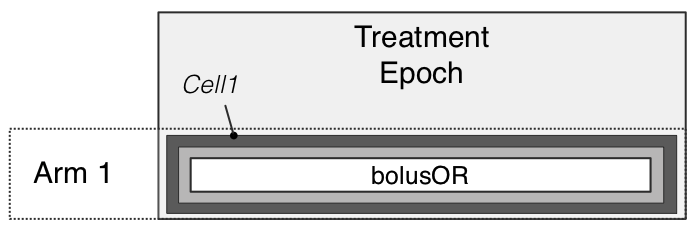
\includegraphics[width=0.7\linewidth]{../pics/OneArmOneEpoch_Bonate}
\caption{Design overview: this study consists of one arm and one epoch.}
\label{fig:designPatternBonate}
\end{figure}

\begin{table}[htdp!]
\begin{center}
\begin{tabular}{ccccccc}
\hline
Segment&Activity & Treatment & DoseTime & DoseSize & Target Variable \\
\hline
TA& bolusOR &  OR bolus & 0 & 100 & D \\
\hline
\end{tabular}
\end{center}
\caption{Segment/activity overview.}
\label{tab:segementActivity_Ribba}
\end{table}

\begin{table}[htdp!]
\begin{center}
\begin{tabular}{ccc}
\hline
Epoch & Start time & End time \\
\hline
Treatment Epoch & 0 &  12  \\
\hline
\end{tabular}
\end{center}
\caption{Epoch definition -- there is only one epoch here.}
\label{fig:Bonate:epochDef}
\end{table}

While the implementation of epoch, arm, cell and segment is analog to that in the 
previous example, the \xelem{Activity} element contains new items. After we 
defined \xelem{DoseAmount} as before as well, the steady-state administration 
is easily implemented using the \xelem{SteadyState} with last doing event as
\xelem{EndTime} and the dose interval as \xelem{Interval} as can be seen 
in the following listing \inputxml{bonate_activity.xml}



%%%%%%%%%%%%%%%%%%%%%%%%%%%%%%%%%%%%%%%%%%%%%%%%%%%%%%%%%%%%%%%%
%%%%%%%%%%%%%%%%%%%%%%%%%%%%%%%%%%%%%%%%%%%%%%%%%%%%%%%%%%%%%%%%
%%%%%%%%%%%%%%%%%%%%%%%%%%%%%%%%%%%%%%%%%%%%%%%%%%%%%%%%%%%%%%%%
\eglabel{4}
\section{Example \theexamples: Estimation, Warfarin PK}
\label{sec:eg4}

\subsection{Description}

This model describes the PK of the drug Warfarin and corresponds to
the \ddmore WP3 use case Warfarin\_PK\_PRED\footnote{\raggedright Available via Interface Europe: \url{https://cp1.interfaceurope.eu/LotusQuickr/ddmore/PageLibraryC125786900388659.nsf/h_Toc/92be13faec1b58390525670800167238/?OpenDocument\#{type=0\&unid=5801C48FC6C39BB141257B2A007D6F31}}}. 

\subsubsection{Structural model}

The model is a one compartment model with first-order absorption with
lag time and first-order elimination.

\begin{description}
\item[\itshape D] Dosing variable.
\item[\itshape t\textsubscript{D}] Time of the dose.
\item[\itshape C] Concentration of drug in the compartment.
\end{description}
\begin{align*}
k &= \frac{\CL}{V}\\
C(t) &= \begin{cases}
  0 & \text{if } \quad t - t_D < \Tlag \\
  \frac{D}{V}\frac{k_a}{k_a-k}\left[e^{-k\,
       \left(t-t_D-T_{lag}\right)}-e^{-k_a \, \left(t-t_D-T_{lag}\right)}\right] &
  \text{otherwise}
\end{cases}
\end{align*}


\subsubsection{Covariate model}

%The covariate is Weight, $W$, a continuous covariate with the following transformation applied:
%\begin{gather}
%%W \sim \mathcal{N}(\pop_{\Weight}, \omega_{\Weight})
%\log(\Weight/70) \nonumber
%%\intertext{initial values:}
%%\pop_{\Weight} =70.07, \quad \omega_{\Weight} =14.09 \nonumber
%\end{gather}
%
Body weight, $W$, is the only continue covariate used in this model. It is used in the model
for the individual clearance and volume.
\begin{table}[h]
\begin{center}
\begin{tabular}{lr}\toprule
 & \textbf{Weight} \\\midrule
Type & Continues \\
Transformation & $\log(\Weight/70)$ \\
\bottomrule
\end{tabular}
\end{center}
\caption{Covariates overview.}
\label{tab:CovariatesOverview}
\end{table}




\subsubsection{Parameters}

\paragraph{PK Parameters}

The following PK parameters are used in the model:
\begin{description}
\item[\Tlag] The lag time.
\item[\ka] The absorption rate constant.
\item[\var{V}] The volume of distribution.
\item[\CL] Clearance of elimination.
\end{description}

\begin{align*}
\intertext{The parameters are defined as follows:}
\log(\Tlag) &= \log(pop\_\Tlag) + \eta_\Tlag\\
\log(\ka) &= \log(pop\_\ka) + \eta_\ka\\
\log(\var{V}) &= \log(pop\_\var{V}) + \beta_{1,V} \log(W_i/70) + \eta_\var{V}\\
\log(\CL) &= \log(pop\_\CL) + \beta_{1,\CL} \log(W_i/70) + \eta_\CL
\end{align*}
where
\begin{gather*}
\eta_\Tlag \sim \mathcal{N}(0, \omega_{\Tlag}), \quad \eta_\ka \sim \mathcal{N}(0, \omega_{\ka}),\\
\eta_\var{V} \sim  \mathcal{N}(0, \omega_{V}), \quad \eta_\CL \sim \mathcal{N}(0, \omega_{\CL})
\end{gather*}
Note please that, in this case, $\beta_{1,V}=0.75$ and $\beta_{1,CL}=1$, i.e. are fixed and will not be estimated.

\paragraph{Variance-covariance matrix}
The full variance-covariance matrix for the random effects is :
\begin{equation*}
 \Omega =
 \begin{pmatrix}
  \omega_{Tlag}^2 	& 0 				& 0                                 & 0  \\
   			  	& \omega_{\ka}^2	& 0                                 & 0  \\
  				& 				& \omega_{\var{V}}^2     & 0  \\
 				&				&                                    & \omega_{\CL}^2 \\
 \end{pmatrix}
%\label{sec:eg-covariance-mat}
\end{equation*}

\subsubsection{Observation model}

We apply a residual error models to the output variable \var{C}.

%\noindent
\begin{center}
\begin{tabular*}{0.6\textwidth}{@{\extracolsep{\fill}} >{\bfseries}l l}\toprule
Output Variable  & \textbf{\itshape C} \\\midrule
Observations Name & Concentration\\
Units & $\mg/l$ \\
Observations Type & Continuous \\
Residual Error Model & Combined2 \\
Error Model Parameters & $a = 0.1,\quad b=0.1$\\
\bottomrule
\end{tabular*}
\end{center}

\subsubsection{Trial Design}
\label{sec:eg4-trial-design}

The dosing regimen for the trial is given below --- there is only one
for each arm. Note that all dosing is bolus dosing (discrete
administration at specific times) and all doses are administered to
the same compartment.

%\noindent
\begin{center}
\begin{tabular*}{0.45\textwidth}{@{\extracolsep{\fill}} >{\bfseries}l r}\toprule
Arm & \textbf{1} \\\midrule
Number of subjects & 33\\
Dose variable & \var{D} \\
Dosing Amount & 100 \\
Dose Units & $\mg$  \\
Dose per kg & no \\
Dosing times (h) & 0\\
\bottomrule
\end{tabular*}
\end{center}

% The trial is has just one study group of 33 individuals.
% \begin{align*}
% \DoseTime (t_D)&= 0    \\
% \TimeUnit&= h
% \intertext{Dosing is adjusted to body weight}
% \DoseSize&= 100  \\
% \DosePerKg&=\no   \\
% \DoseUnit&=\mg
% \intertext{Time of measurement for PK}
% \ObservationTime&= 0.5,1,2,3,6,9,24,36,48,72,96,120
% \end{align*}

\subsubsection{Modelling Steps}

The observations for the output variable is shown below. These
time-points correspond to those define in the data-file. The task to
be performed is a parameter estimation which will involved the
following steps:
\begin{itemize}
\item Estimation of population paramaters.
\item Estimation of Fisher information matrix.
\item Estimation of the individual parameters.
\end{itemize}

%\noindent
\begin{center}
\begin{tabular*}{0.6\linewidth}{@{\extracolsep{\fill}} >{\bfseries}l c}\toprule
Output Variable & \textbf{\itshape C}\\
Observation times & 0.5,1,2,3,6,9,24,36,48,72,96,120\\
\bottomrule
\end{tabular*}
\end{center}

\begin{figure}[ht!]
\centering
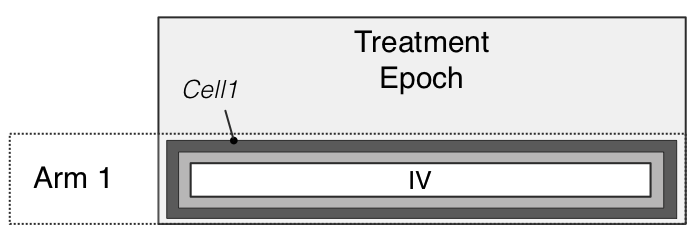
\includegraphics[width=0.7\linewidth]{../pics/designPattern_1Arm1Epoch}
\caption{Design overview: this study consists of one arm and one epoch.}
\label{fig:designPattern_1Arm1Epoch}
\end{figure}

Figure \ref{fig:designPattern_1Arm1Epoch} shows the \textit{Structure} of
this simple example consisting of 1 arm and one epoch, meaning one treatment
type for everybody.

%
% The output variable is:
% \begin{description}
% \item[\var{C}] Concentration in the central compartment, in this case
%     the bloodstream.
% \end{description}

\subsection{Overview}

This our first estimation case. From figure \ref{fig:simEstTasks_List} 
it follows that we can expect significant differences in the Trial Design and Modelling Steps
sections compared to the previous simulation case.

%, see listing \ref{fig:exp5_modelOverview}
%for an overview.

Accordingly, the Model Definition is very similar to that in the
previous example.  The main \pharmml feature we have not seen
previously is the algebraic structural model (i.e., the model is not
defined as a system of ODEs). The XML is too long to show here and is
similar to the examples shown previously (section \ref{sec:maths}). If
you are interested then please consult the full example associated
with this specification.

We will start with the description of the Trail design. Note that because
every subject receives the same dosing regimen, this can be encoded 
in the \xelem{Activity} block. Otherwise we would have to define the 
individual dosing regimens in the \xelem{IndividualDosing} element, see
section \ref{subsubsec:Ribba_indivDosing} in example \ref{sec:Ribba} how
this is done.

%\begin{listing}[htb]
%\inputxml{exp5_modelOverview.xml}
%\caption{Defining the complete model.}
%\label{fig:exp5_modelOverview}
%\end{listing}


\subsection{Trial Design}
\label{eg4_subsec:trialDesign}
\subsubsection{Structure}

As explained in the chapter \ref{sec:CTS} on trial design, we base the following 
structure on the CDISC standard Study Design Model \cite{CDISC:2011a}. 
The design elements are contained in the \xelem{Structure} block and you can see 
in following listing \inputxml{exp5_structure.xml}
how the study is constructed of a single epoch, 
with a single arm and a single cell that contains a single segment. Note, though 
that this structure is not hierarchical and the \xelem{Cell} element joins the arm, 
epoch and segments together. 

The last section of the structure, the \xelem{Activity} element, is of interest for 
the discussion. This is because, as already mentioned above, the administration
and dosing regimen is identical for every patient. The dose amount is $D=100\; mg$ 
and the dose time is $t_D=0$.
As in the previous example, the structural model is defined using an algebraic
function with the dosing variable \var{D} which means the \xelem{DoseAmount} element
has the attribute \xatt{inputType="dose"}. Additionally the dosing time variable \var{tD} is
referenced here and initialised. 


%\begin{listing}[htb]
%\inputxml{exp5_structure.xml}
%\caption{Structure overview.}
%\label{lst:exp5_structure}
%\end{listing}

\subsubsection{Population}

This is the place where we describe the individuals in the study, which 
\var{Arm} they belong to and any possible individual characteristics, such as 
body weight, age and other covariates. In this example we only know the
body weight of the subjects. 
We define the known attributes of all individuals using the 
\xelem{IndividualTemplate} and then map each individual to this template 
using a \xelem{Dataset}. In the following listing \inputxml{exp5_population.xml}
you can see how this 
is implemented in \pharmml. Column \var{2} in the table is equal for
every subject because they all belong to one arm, here denoted as \var{a1}.

%\begin{listing}[htb]
%\inputxml{exp5_population.xml}
%\caption{Population overview.}
%\label{fig:exp5_population}
%\end{listing}

\subsection{Modelling Steps}

\subsubsection{Objective data}

The biggest advantage of the current specification is that we do not have
to define the design in the data file. After the structure of the trial is defined
as above we just need to encode the measured experimental data, here the time 
and the independent variable, the concentration values. To achieve that we 
define a table in \xelem{Dataset} with columns: \var{ID}, \var{time} and 
\var{dv} and populate it with given experimental values, see \xelem{ObjectiveDataSet} block 
in the following listing \inputxml{exp5_objDataSet.xml}
Before that we have to make sure that these values are correctly mapped to 
variable used in the model which is implemented in the \xelem{VariableMapping}
element. Accordingly, we define the identifier \var{ID} and 
define the variable mapping. Here the \var{time} as in the data is mapped 
to model time \var{t} and the measured concentration is mapped to the 
variable \var{C} as in the observation model.


%\begin{listing}[htb]
%\inputxml{exp5_objDataSet.xml}
%\caption{Objective dataset overview.}
%\label{fig:exp5_objDataSet}
%\end{listing}	

\subsubsection{Parameter estimation}


In a parameter estimation you do not necessarily want to estimate all
the parameters in your model or you may wish to define bounds within
which your parameter should be estimated, or provide an initial
estimate.  The \xelem{ParametersToEstimate} element controls this. As
you can see in the following listing \inputxml{exp5_paramEstimation.xml}
we use a \xelem{ParameterEstimation} element that refers to the parameter in
the model definition.  In its simplest form you can decide whether the
parameter is to be estimated by setting the \xatt{fixed} attribute
(false indicates the parameter should be estimated). If a parameter is
not defined here, then it is assumed that it will not be estimated, in
which case it would be assigned an initial value elsewhere in the
PharmML document.  One of the validation rules (see chapter
\ref{chapter:validation}) is that every parameter has to be
initialised. 
%This can happen either in the \xelem{ParameterModel},
%\xelem{ObservationModel} or in this \xelem{ParametersToEstimate} block.
 

%\subsubsection{Operation}
%
%\begin{listing}[htb]
%\inputxml{exp5_operation.xml}
%\caption{Operation overview.}
%\label{fig:exp5_operation}
%\end{listing}


\subsubsection{Step dependencies}

Then at the end of the \xelem{ModellingSteps} block is the \xelem{StepDependencies} element. 
This describes the ordering of the steps in the modelling process, but in this case it is 
almost trivial as we only have one step in this example:
\inputxml{exp5_steps.xml}


%\begin{listing}[htb]
%\inputxml{exp5_steps.xml}
%\caption{Step dependencies overview.}
%\label{fig:exp5_steps}
%\end{listing}






%%%%%%%%%%%%%%%%%%%%%%%%%%%%%%%%%%%%%%%%%%%%%%%%%%%%%%%%%%%%%%%%
%%%%%%%%%%%%%%%%%%%%%%%%%%%%%%%%%%%%%%%%%%%%%%%%%%%%%%%%%%%%%%%%
%%%%%%%%%%%%%%%%%%%%%%%%%%%%%%%%%%%%%%%%%%%%%%%%%%%%%%%%%%%%%%%%
\eglabel{6}
\section{Example \theexamples: Estimation with IOV}
\label{sec:eg6}

%%%%%%%%%%%%%%%%%%%%%%%%%%%%%%%%%%%%%%%%%%%%%%%%%%%%%%%%%%%%%%%%
\subsection{Description}

In this example we will look at more complex trial design and a
correspondingly complex variability model. The model also includes
categorical covariates, which is again something we have not
encountered thus far. The example is based on example IOV1 from
Monolix 4.1 (see \cite{Monolix4.1.4UserGuide:2012} for a detailed
description) and features a cross-over design and inter-occasion
variability (see section \ref{sec:variabilityModel}). As before we will
go through the key elements of the model before we look at the
\pharmml examples, but given the complex nature of the trial design we
will describe that first then move onto the model definition.


\begin{figure}[htb]
\centering
 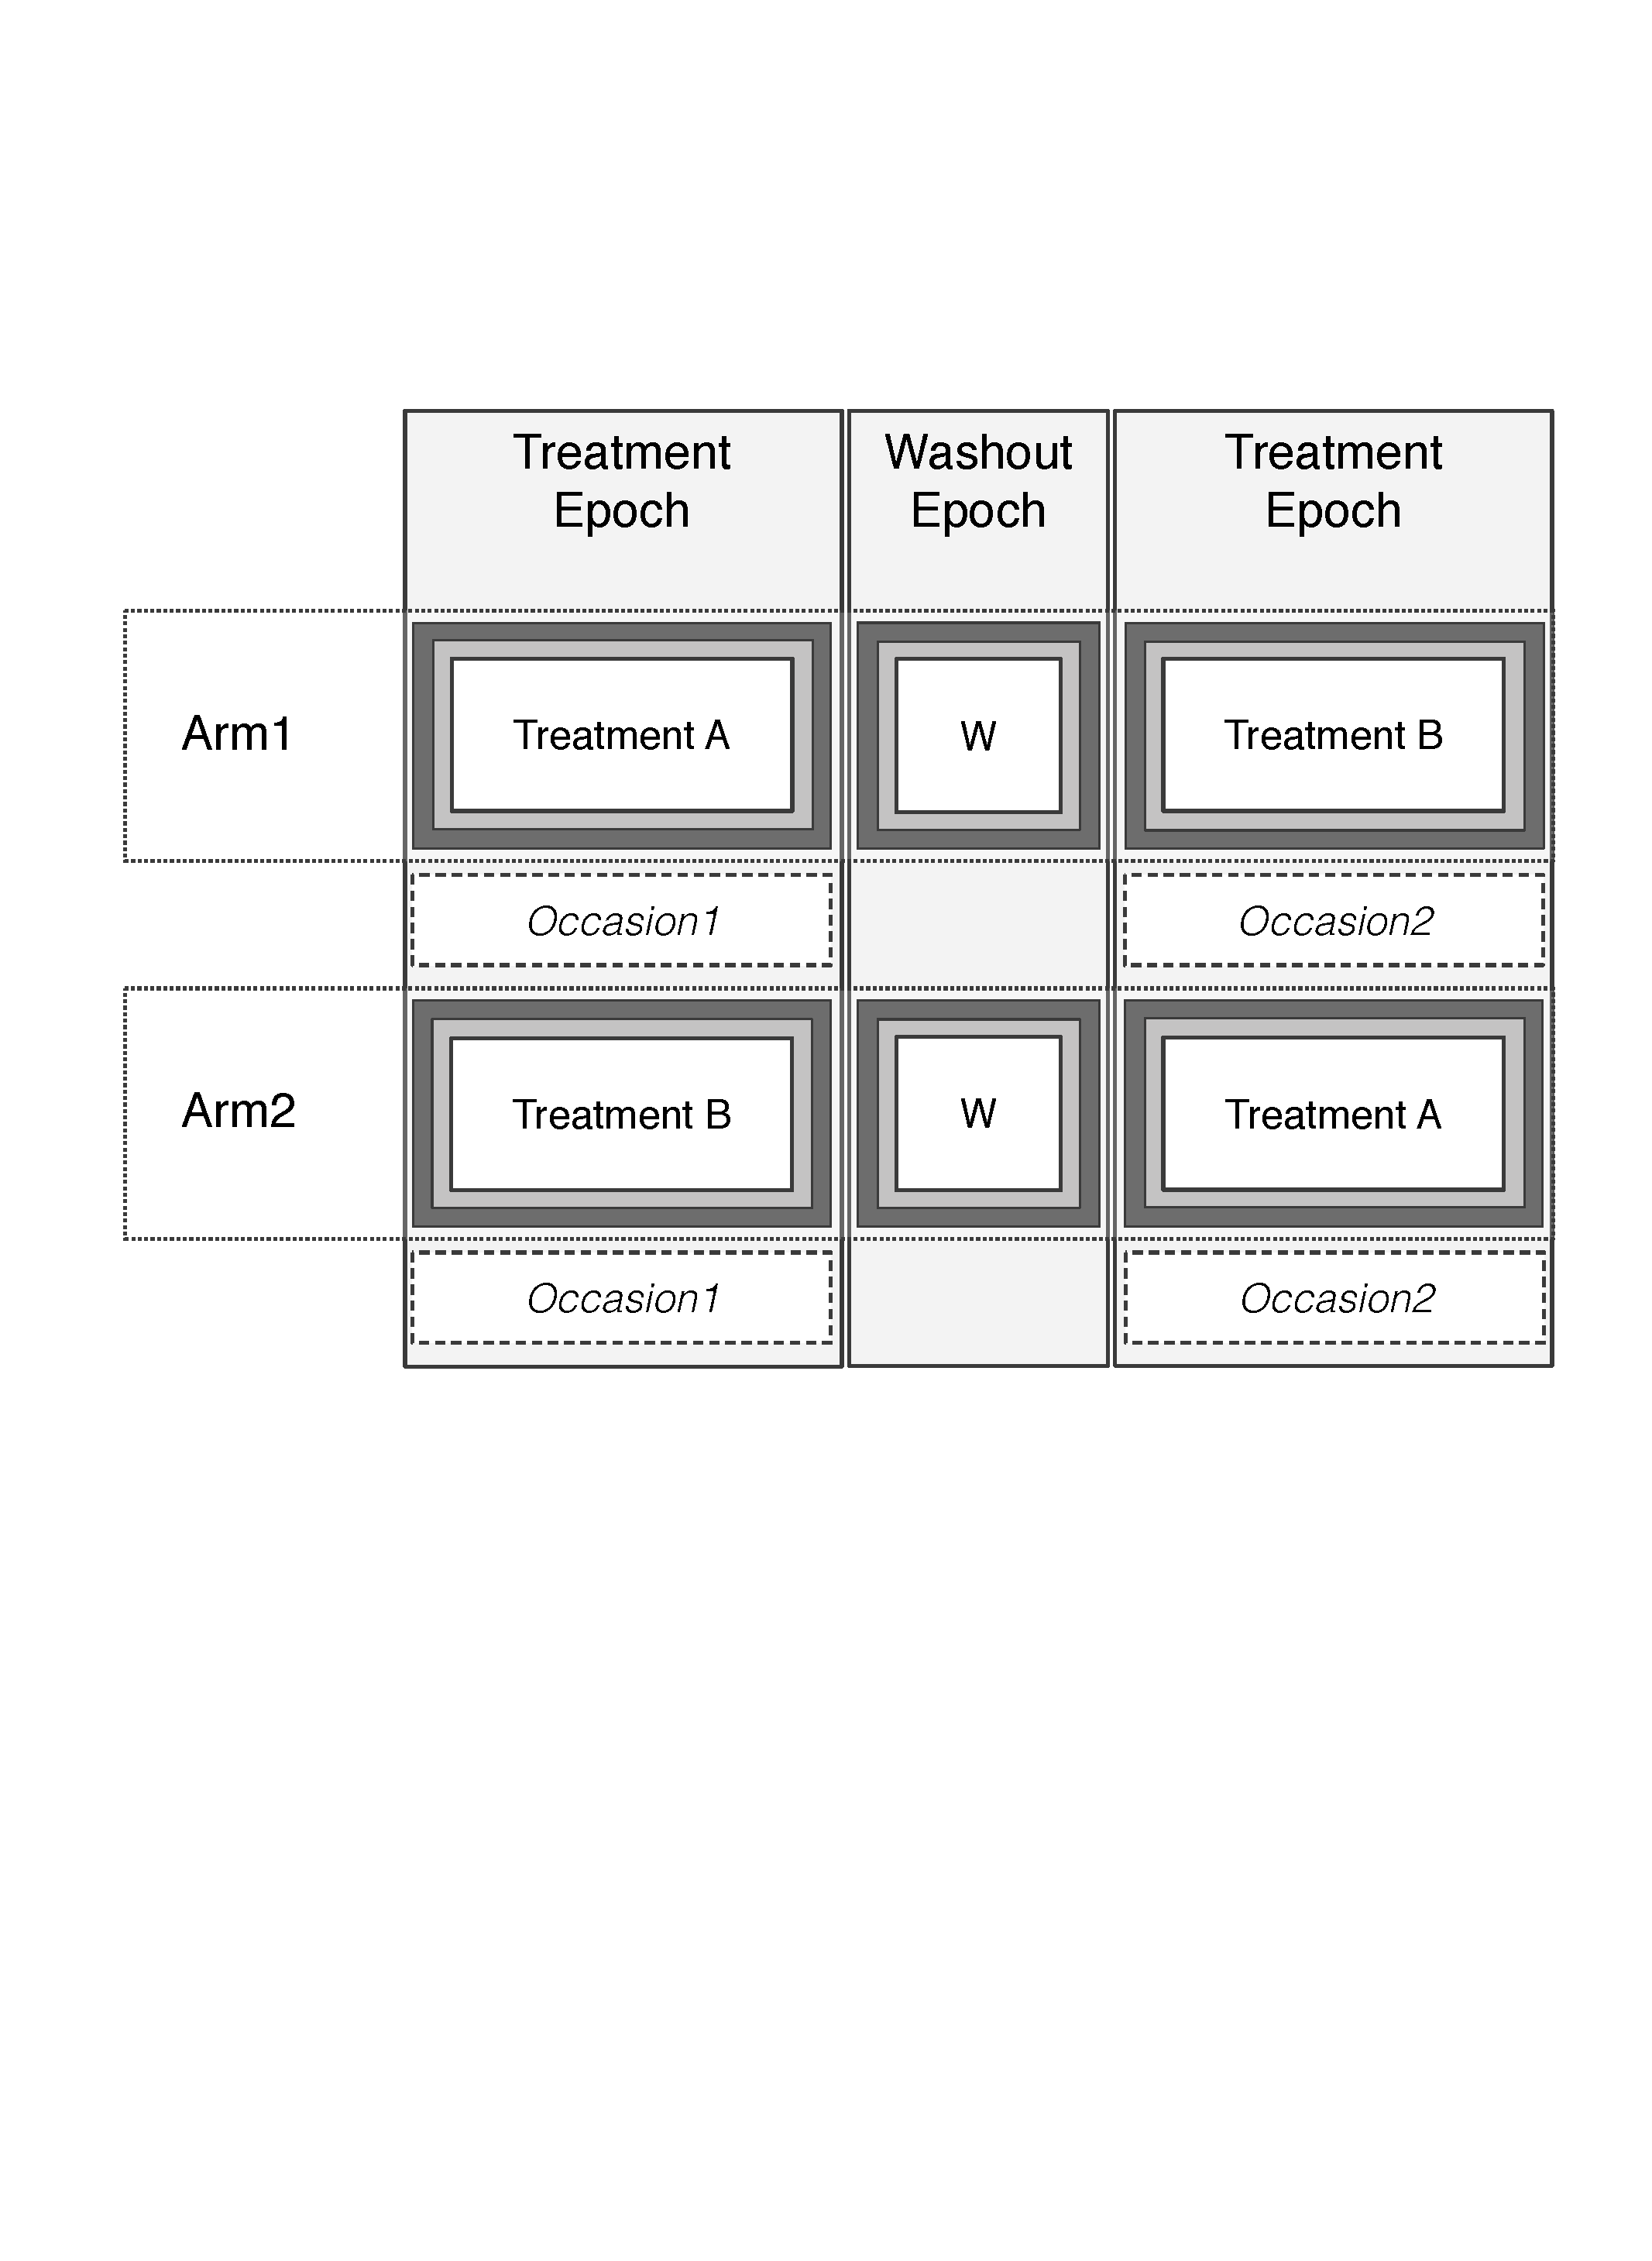
\includegraphics[width=0.7\linewidth]{TwoArmsThreeEpochs_withWashout.pdf}
\caption{Schematic representation of a crossover design with washout. The reader is referred to
Figure \ref{fig:templateTrialDesign} for the colour code used to identify the elements of
a trial. See tables \ref{fig:eg6:segmentCellArmEpoch} 
and \ref{fig:eg6:epochDef} for the detailed definition of segments, cells, arms, epochs
and occasions in this example.}
\label{fig:TwoArmsThreeEpochs_withWashout}
\end{figure}

%\noindent
\begin{table}[h]
\begin{center}
\begin{tabular}{lrr}\toprule
Arm & \textbf{1} & \textbf{2} \\\midrule
Number of subjects & 33 & 33\\
Dose variable & \var{D} & \var{D} \\
Dosing Amount & 100 & 150 \\
Dose Units & $\mg$ & $\mg$  \\
Dose per kg & no & no \\
Dosing times (h) &  [0 : 12 : 72] &  [0 : 12 : 72\\
\bottomrule
\end{tabular}
\end{center}
\caption{Arms overview with dosing specification.}
\label{tab:ArmOverview}
\end{table}


%%%%%%%%%%%%%%%%%%%%%%%%%%%%%%%%%%%%%%%%%%%%%%%%%%%%%%%%%%%%%%%%
\subsubsection{Trial Design}
The model features a basic crossover design (see Figure
\ref{fig:TwoArmsThreeEpochs_withWashout}) with washout period and inter-occasion
variability (IOV). There are two treatments and the subjects are
organised into two arms that start with a different treatment. In
between each treatment there is a washout period during which time the
drug is eliminated from each subject. 
In the model the treatments, fi treated as occasions, provide a second level of variability -- 
IOV \index{variability!IOV} (see section \ref{sec:variabilityModel}).  
This is summarised in Figure \ref{fig:eg6-IOV_2levels} (see also the listing 
in section \ref{eg6:variabilityModel}, showing relevant code 
within the element \xelem{VariabilityModel}).

The model also uses covariates to model the variability within the
model and so the treatments, the sequence of treatments (i.e.\xspace treatments A, B or
B,A) and the occasion itself are described in the covariate section
below.

\begin{figure}[ht!]
\centering
 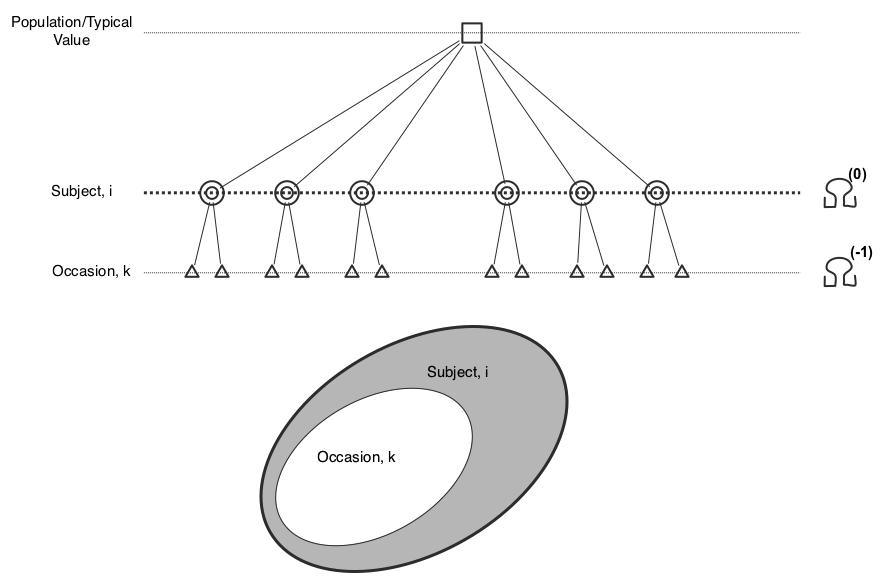
\includegraphics[width=120mm]{IOV_2levels}
\caption{Two levels of variability -- inter-individual and inter-occasion within individual variability.}
\label{fig:eg6-IOV_2levels}
\end{figure}


%%%%%%%%%%%%%%%%%%%%%%%%%%%%%%%%%%%%%%%%%%%%%%%%%%%%%%%%%%%%%%%%
\subsubsection{Covariate Model}
\label{eg6:covariates-defn}

As discussed about all but the `Sex' covariate is used to capture the
variability in the model, see Table \ref{tab:CovariatesOverview}.

\begin{table}[h]
\begin{center}
\begin{tabular}{lrrrr}\toprule
 & \textbf{Sex} &{\color{red}\textbf{Treat}}&{\color{mediumgreen}\textbf{TreatSeq}}&{\color{magenta}\textbf{Occasion}}\\\midrule
Type & Categorical & Categorical & Categorical & Categorical  \\
Category Count & 2 & 2 & 2 & 2\\
Categories & F, M & A, B & A--B,B--A & 1, 2\\
Reference & F & A & A--B & 1\\
%Reference Probability & $14/36$ & 0.5  & 0.5  & 0.5\\
\bottomrule
\end{tabular}
\end{center}
\caption{Covariates overview.}
\label{tab:CovariatesOverview}
\end{table}

%%%%%%%%%%%%%%%%%%%%%%%%%%%%%%%%%%%%%%%%%%%%%%%%%%%%%%%%%%%%%%%%
\subsubsection{Parameter Model}

The parameter model includes random effects that represent the IIV and
{\color{lightblue}IOV} levels of variability. It also relates the
parameters to the covariates described above\footnote{To improve
  clarity we have colour coded the contributions of the different levels
of variability and the different covariates.}

\begin{align}
\log(ka_{i}) &= \log(ka_{pop}) +
{\color{mediumgreen}\beta_{ka,TreatSeq}}1_{TreatSeq_i=A-B} +
\eta_{ka,i} \label{eqn:eg6-param-ka}\\
\begin{split}
\log(V_{ik}) &= \log(V_{pop}) + {\boldsymbol \beta_V}1_{S_i=F} +
{\color{magenta}\beta_{V,OCC}} 1_{OCC_{ik}=1} \\
&\quad+ {\color{red}\beta_{V,Treat}}1_{Treat_{ik}=A} + {\color{mediumgreen}\beta_{V,TreatSeq}}1_{TreatSeq_i=A-B} \\
		& \quad+ \eta_{V,i}^{(0)} +  {\color{lightblue} \eta_{V,ik}^{(-1)} }
\end{split} \label{eqn:eg6-parameter-v}\\
\begin{split}
\log(\CL_{ik}) &= \log(\CL_{pop}) + {\boldsymbol \beta_{\CL}}1_{S_i=F}
+ {\color{magenta}\beta_{\CL,OCC}} 1_{OCC_{ik}=1}\\
&\quad + \eta_{\CL,i}^{(0)} + {\color{lightblue} \eta_{Cl,ik}^{(-1)} }
\end{split}\nonumber
\end{align}
where
\begin{gather*}
\eta_{ka,i}^{(0)} \sim \mathcal{N}(0, \omega_{ka}), \quad \eta_{V,i}^{(0)} \sim \mathcal{N}(0, \omega_{V}), \quad \eta_{\CL,i}^{(0)} \sim \mathcal{N}(0, \omega_{\CL}),  \\
 {\color{lightblue} \eta_{V,ik}^{(-1)} \sim \mathcal{N}(0,\gamma_V)}, \quad
 {\color{lightblue} \eta_{\CL,ik}^{(-1)} \sim \mathcal{N}(0, \gamma_{\CL})}
\end{gather*}

The full variance-covariance matrix for our model is :
\begin{gather}
 \Omega^{(0)} =
 \begin{pmatrix}
  \omega_{ka}^2 	& 0 				& 0  \\
   			  	& \omega_{V}^2	& 0 	\\
  				& 				& \omega_{\CL}^2\\
 \end{pmatrix}\label{eqn:eg6-covariance-mat}\\
 \Omega^{(-1)} =
 \begin{pmatrix}
0 & 0 & 0\\
 & \gamma_{V}^2	& 0 	\\
 & & \gamma_{\CL}^2\\
 \end{pmatrix}\label{eqn:eg6-gamma-mat}
\end{gather}


%%%%%%%%%%%%%%%%%%%%%%%%%%%%%%%%%%%%%%%%%%%%%%%%%%%%%%%%%%%%%%%%
\subsubsection{Structural model}

The model is first order absorption with linear elimination, with
multiple dosing. This is the equivalent to oral1\_1cpt\_kaVCl (model 8) from \cite[Appendix I]{Bertrand:2008}.


%%%%%%%%%%%%%%%%%%%%%%%%%%%%%%%%%%%%%%%%%%%%%%%%%%%%%%%%%%%%%%%%
\subsubsection{Observation model}

We apply a residual error models to the output variable \var{C}.

%\noindent
\begin{center}
\begin{tabular*}{0.6\textwidth}{@{\extracolsep{\fill}} >{\bfseries}l l}\toprule
Output Variable  & \textbf{\itshape C} \\\midrule
Observations Name & Concentration\\
Units & $\mg/l$ \\
Observations Type & Continuous \\
Residual Error Model & Combined \\
Error Model Parameters & $a = 0.1,\quad b=0.1$\\
\bottomrule
\end{tabular*}
\end{center}


%%%%%%%%%%%%%%%%%%%%%%%%%%%%%%%%%%%%%%%%%%%%%%%%%%%%%%%%%%%%%%%%
\subsubsection{Modelling Steps}
Compared to the last example, we have define here two tasks:
\begin{itemize}
\item Estimation of population paramaters.
\item Estimation of the individual parameters.
\end{itemize}

%%%%%%%%%%%%%%%%%%%%%%%%%%%%%%%%%%%%%%%%%%%%%%%%%%%%%%%%%%%%%%%%
\subsection{Trial Design}

We have summaries the dosing regimen and organisation of the trial
design below, see also Figure \ref{fig:TwoArmsThreeEpochs_withWashout}.

\begin{table}[htdp!]
\begin{center}
\begin{tabular}{ccccccc}
\hline
Segment&Activity & Treatment & DoseTime & DoseSize & Target Variable \\
\hline
TA& OR1 &  OR bolus & $0:12:72$ & 150 & Ac \\
TA& OR2 &  OR bolus & $0:24:72$ & 100 & Ac \\
\hline
\end{tabular}
\end{center}
\caption{Segment/activity overview.}
\label{fig:eg6:segmentCellArmEpoch}
\end{table}

\begin{table}[htdp!]
\begin{center}
\begin{tabular}{cccc}
\hline
Epoch & Occasion & Start time & End time \\
\hline
Treatment Epoch & OCC1 & 0 &  180  \\
Washout & -- & 0 &  10  \\
Treatment Epoch & OCC2 & 0 &  180  \\
\hline
\end{tabular}
\end{center}
\caption{Epoch and occasion definition.}
\label{fig:eg6:epochDef}
\end{table}


%%%%%%%%%%%%%%%%%%%%%%%%%%%%%%%%%%%%%%%%%%%%%%%%%%%%%%%%%%%%%%%%
\subsubsection{Structure}
The implementation of the treatments, in \pharmml we use the
\xelem{Activity} element, is different compared to the previous example. 
See Table \ref{fig:eg6:segmentCellArmEpoch} for the details. The difference
is that now we have one dose administered at multiple dosing time points 
instead of single time point. See the following listing \inputxml{exp6_dosingTimes.xml}
how one can describe it within the \xelem{DosingTimes} element using the \xelem{Sequence}
structure defining the start/end times and step size.

Table \ref{fig:eg6:epochDef} gives an overview of the \var{Epochs} and \var{Occasions} 
in this example. Here, the occasions overlap with the epochs, the start and end times 
are identical, this is not always the case, the occasions can span one or more epochs. 
The \var{Washout} epoch is given here with start/end times as well which is in fact 
a redundant piece of information (but required by construction of an \var{Epoch})
as a \var{Washout} always assumes total reset of all drug amounts. 

%\begin{listing}[ht!]
%\inputxml{exp6_structure_part3.xml}
%\caption{The implementation of the mapping of IOV to the trial design.}
%\label{exp6_structure_part3}
%\end{listing}

As discussed in the section \ref{subsec:TrialStructure}, in \xelem{Structure} block 
we encode the variability which is located below the subject (see the 
hierarchy of the random variability discussed in section \ref{sec:variabilityModel}).
We call it the \textit{inter-occasion variability}, IOV. The following listing 
\inputxml{exp6_structure_part3.xml} shows how this is done. 
In this case the occasions coincide with the epochs 
so we use the \xelem{EpochRef} element. Alternatively, we could use the \xelem{Period}
element to define explicitly the start and end times of the occasions as shown 
in this listing: \inputxml{exp6_structure_part4.xml}
This is of course very useful if the occasions do not
coincide with the epochs, or there are two or more occasions within one epoch.
In this case we set the \var{Start} and \var{End} times to $0$ and $180$, respectively.
These are exactly the same time points as are used in the epoch definition 
(see the first listing in section \ref{eg4_subsec:trialDesign} for how to encode epochs in the 
\xelem{Structure} definition).   

%\begin{listing}[ht!]
%\inputxml{exp6_structure_part4.xml}
%\caption{Alternative implementation of the mapping of IOV to the trial design shown in previous listing.}
%\label{exp6_structure_part4}
%\end{listing}
 

%%%%%%%%%%%%%%%%%%%%%%%%%%%%%%%%%%%%%%%%%%%%%%%%%%%%%%%%%%%%%%%%
\subsubsection{Population}
We pick up where we left off in the \xelem{Structure}, implementing
the hooks to the variability structure. The aspect we have not covered
yet is related to IIV.  The \xelem{Population} element is the place to
define any subject related variability and those levels above
it. The following listing shows how this works \inputxml{exp6_population_part0.xml}
Here we deal only with the IIV so we are done with this aspect.

%\begin{listing}[ht!]
%\inputxml{exp6_population_part0.xml}
%\caption{The implementation of the IIV mapping.}
%\label{exp6_population_part0}
%\end{listing}

The next part of the \xelem{Population} block was discussed previously, 
with one exception. Beside the standard assignment of subjects to an \var{Arm}
and providing information regarding \var{Sex}, we need to encode the information
about \var{Treat}, i.e. treatment type considered here as covariate, which varies
by definition in this cross-over design as the study progress from \var{Epoch1}
to \var{Epoch3}. To encode this we use the \textit{nested table} concept as described 
in section \ref{sec:dataset}. 
Here the child table is defined by using a \xelem{Table} element instead of the 
usual \xelem{Column} element and given the identifier 'treat-tab'. 
Within the nested table definition another set of relevant columns is specified, 
\var{epoch} and \var{treat}. Next these nested tables are populated with 
data as can be seen in the following listing \inputxml{exp6_population_part2.xml}
here for \var{Arm1}.
Listing \inputxml{exp6_population_part2B.xml}
shows one data record for \var{Arm2}.

%\begin{listing}[ht!]
%\inputxml{exp6_population_part2.xml}
%\caption{The implementation of the nested table for time varying covariate, \var{Treat}, for  \var{Arm1}.}
%\label{exp6_population_part2}
%\end{listing}

%\begin{listing}[ht!]
%\inputxml{exp6_population_part2B.xml}
%\caption{The implementation of the nested table for time varying covariate, \var{Treat},  for  \var{Arm2}.}
%\label{exp6_population_part2B}
%\end{listing}


%%%%%%%%%%%%%%%%%%%%%%%%%%%%%%%%%%%%%%%%%%%%%%%%%%%%%%%%%%%%%%%%
\subsection{Variability Model}
\label{eg6:variabilityModel}

In this example the variability model is more complex than before, with IIV\index{variability!IIV} and IOV\index{variability!IOV} levels of variability, see Figure \ref{fig:eg6-IOV_2levels}. As you will see, in \pharmml the complexity comes later -- in the parameter model. At this point in the \pharmml document all we need to do is define the variability levels to be used in the rest of the document. You can see in the following listing \inputxml{exp6_iov.xml}
that this is done simply by listing the variability levels using the \xelem{VariabilityLevel} element. There are three important points to note here:
\begin{enumerate}
\item There is parent-child relationship between the levels of variability. The \var{Subject} level, 
in the \pharmml it is referenced with the attribute \xatt{symbId="indiv"} is higher
in the hierarchy and directly above the \var{Occasion} level, referenced with the 
attribute \xatt{symbId="iov1"} which is exactly what is done
using the \xelem{ParentLevel} in the listing above.
\item The name given to a level, using the \xatt{symbId} attribute, is \textbf{not} significant. We used the names \var{iov1} and \var{indiv} to provide clarity in other parts of the example document.
\item the type of each variability level (e.g.,\xspace between-subject, inter-occasion, between-centre) is not defined here or in the Model Definition as a whole\footnote{N.B.,\xspace The numerical levels described in the variability model (section \ref{sec:variabilityModel}) are not used.}.
\end{enumerate}

So in this example the \pharmml document tells us that there are two variability levels and that the lowest level of variability is called ``\texttt{iov1}''\index{variability!IOV}\@. This may seem odd, but to simulate or estimate the model we do not need to know which level of variability is considered IIV and which IOV.  We only need to know their level relative to each other. Of course it may be desirable to know this when exchanging  a model, and we feel that this information can be provided by annotation of the \pharmml document.


%%%%%%%%%%%%%%%%%%%%%%%%%%%%%%%%%%%%%%%%%%%%%%%%%%%%%%%%%%%%%%%%
\subsection{Covariate Model}

The covariate model describes categorical covariates, listed in Table 
\ref{tab:CovariatesOverview}, \index{covariate!categorical}which we have 
not seen in the previous examples. 

Because this is an estimation example no probabilities are provided and only the 
categories are defined, placed in the \xelem{Categorical} element. 
Then the implementation of each covariate follows the same
schema, which will be explained for the gender covariate \var{Sex}. 
There are obviously two categories the covariate can be associate with \textit{F} or \textit{M},
which are encoded using the \xelem{Category} element followed by an optional
\xelem{Name}. 

See the following listing how this is done 
\inputxml{exp6_covariates.xml}

%%% TODO
%%%In a later simulation example (example \egref{8}, section
%%%\ref{eg8:example8}) you will see how to assign probabilities to categorical covariates.


%%%%%%%%%%%%%%%%%%%%%%%%%%%%%%%%%%%%%%%%%%%%%%%%%%%%%%%%%%%%%%%%
\subsection{Parameter Model}

In example \egref{1} (section \ref{sec:eg1}) we showed you how to define an individual
parameter in \pharmml and relate that to a continuous covariate. Now
in this example we will show how \pharmml can be used to describe
parameters that have multiple levels of variability and are related to
categorical covariates\index{covariate!categorical}.


In the following listing \inputxml{exp6_ka.xml} we show the definition of
parameter \var{ka}, which corresponds to (\ref{eqn:eg6-param-ka}). You
should be familiar with this structure by now, but you should take
note of the \xelem{Category} element within the \xelem{FixedEffect}
element. We use this to tell \pharmml that this fixed effect is related
to the ``\texttt{AB}'' category of the \var{TreatSeq} covariate. This
is equivalent to the expression
$\beta_{ka,TreatSeq}1_{TreatSeq_i=A-B}$ in
(\ref{eqn:eg6-param-ka}). Note that it is possible to do this more
than once, for example if the covariate has more than two categories.


Parameter \var{ka} has only one level of variability, but this 
\inputxml{exp6_V_part1.xml} and this listing \inputxml{exp6_V_part2.xml}
show how we describe parameter
\var{V} with both IIV and IOV levels of variability. Very simply we
add a \xelem{RandomVariable} for each level of variability and use
the \xatt{symbIdRef} attribute in the \xelem{RandomEffects} element 
to map the random effect to the appropriate variability model as defined at 
the beginning of the \xelem{ModelDefinition} element. 
Thus \var{eta\_V} and \var{kappa\_V} correspond to the 
random effects $\eta^{(0)}_{V,i}$ and $\eta^{(-1)}_{V,ik}$ in
(\ref{eqn:eg6-parameter-v}). This parameter is related to all four
covariates, but we only show the \var{Sex} covariate. The others
defined in a very similar manner as all the covariates in this model
contain just 2 categories.

%%% TODO
We will not show parameter \var{Cl} as it does not illustrate any new
concepts, nor are any of the random effects in the model
correlated. This does not mean there is no covariance matrix defined
within the \pharmml document. There is. The matrices in
(\ref{eqn:eg6-covariance-mat}) and (\ref{eqn:eg6-gamma-mat}) are
implicitly defined because all the random effects follow a normal
distribution and we can deduce the diagonal of each matrix at each
level of variability from the definition of each random effect.

\subsection{Covered in previous examples}
The remaining elements of this example to be encoded in \pharmml
are nearly identical to those described before, such as \xelem{EstimationStep}
and \xelem{StepDepend\-encies} within the\\ \xelem{ModellingSteps} block,
and will not be discussed here.



%%%%%%%%%%%%%%%%%%%%%%%%%%%%%%%%%%%%%%%%%%%%%%%%%%%%%%%%%%%%%%%%%
%%%%%%%%%%%%%%%%%%%%%%%%%%%%%%%%%%%%%%%%%%%%%%%%%%%%%%%%%%%%%%%%%
%%%%%%%%%%%%%%%%%%%%%%%%%%%%%%%%%%%%%%%%%%%%%%%%%%%%%%%%%%%%%%%%%
%\eglabel{4}
%\section{Example \theexamples: Simulation with IOV}
%\label{sec:eg4}




%%%%%%%%%%%%%%%%%%%%%%%%%%%%%%%%%%%%%%%%%%%%%%%%%%%%%%%%%%%%%%%%
%%%%%%%%%%%%%%%%%%%%%%%%%%%%%%%%%%%%%%%%%%%%%%%%%%%%%%%%%%%%%%%%
%%%%%%%%%%%%%%%%%%%%%%%%%%%%%%%%%%%%%%%%%%%%%%%%%%%%%%%%%%%%%%%%
\eglabel{5}
\section{Example \theexamples: Estimation with individual dosing}
\label{sec:Ribba}

%%%%%%%%%%%%%%%%%%%%%%%%%%%%%%%%%%%%%%%%%%%%%%%%%%%%%%%%%%%%%%%%
\subsection{Description}
This example is based on \cite{Ribba:2012uq} and deals with a mathematical
model describing the inhibition of the tumour growth of low-grade glioma treated
with chemotherapy. Although previous estimation examples were complex
enough to illustrate most important aspects of the current \pharmml specification we would
like briefly to discuss this example due to its role as a use case. It also illustrates a new feature
of the language, the fact that we can encode patient specific administration scenarios.


%%%%%%%%%%%%%%%%%%%%%%%%%%%%%%%%%%%%%%%%%%%%%%%%%%%%%%%%%%%%%%%%
\subsection{Trial design}
We will start with the definition of \xelem{Structure}, \xelem{Population}. The next language element, \xelem{IndividualDosing}, is, as mentioned above, new but it's easy to understand.

%%%%%%%%%%%%%%%%%%%%%%%%%%%%%%%%%%%%%%%%%%%%%%%%%%%%%%%%%%%%%%%%
\subsubsection{Structure}
Figure \ref{fig:1Arm1Epoch_RibbaDesign} shows the design structure of this example 
consisting of one arm and one epoch, meaning there is one treatment type 'IV' for all patients. 
As explained in section \ref{sec:CTS} the design element \xelem{Cell} comprises the 
essential elements specifying the information about the arm, epoch and segment/activities. 
\xelem{Segment} contains treatment definition, here an IV bolus administration, 
defined in the \xelem{Activity} element. Figure \ref{fig:cellHierarchy_Ribba} shows 
the general relationship of these elements (left) and how it applies to the current example (right).
See the following listing 
\inputxml{Ribba_structure.xml}
%\caption{Defining \textit{Structure} of the example, i.e. \textit{Epoch}, \textit{Arm}, \textit{Cell} and \textit{Segment}. \textit{Segment} contains \textit{Activity} definition, here a bolus administration.}
%\label{lst:Ribba_structure}
%\end{listing}
for the PharmML implementation.

\begin{figure}[ht!]
\centering
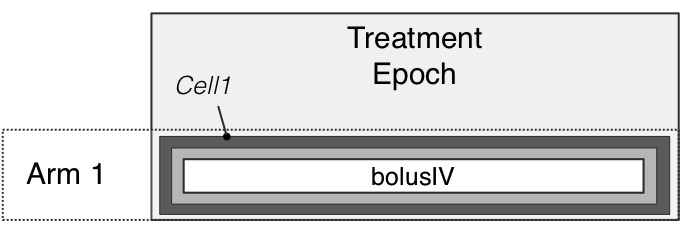
\includegraphics[width=0.7\linewidth]{pics/designPattern_1Arm1Epoch_Ribba}
\caption{Design overview: single arm design.}
\label{fig:1Arm1Epoch_RibbaDesign}
\end{figure}

\begin{figure}[ht!]
\centering
\includegraphics[width=0.7\linewidth]{pics/cellHierarchy_Ribba}
\caption{General cell hierarchy (left); The root of the trial design structure hierarchy is the 'Cell' which can contain one 'Segment',
one 'Epoch' and multiple 'Arms'. The 'Segment' element can have multiple child elements, the 'Activities', e.g. treatments or a washout. (right) An example of how it is applied in \cite{Ribba:2012uq}.}
\label{fig:cellHierarchy_Ribba}
\end{figure}

\begin{table}[htdp!]
\begin{center}
\begin{tabular}{ccccccc}
\hline
Segment&Activity & Treatment & DoseTime & DoseSize & Target Variable \\
\hline
TA& bolusIV &  IV bolus & individual & 1 & C \\
\hline
\end{tabular}
\end{center}
\caption{Segment/activity overview.}
\label{tab:segementActivity_Ribba}
\end{table}

%%%%%%%%%%%%%%%%%%%%%%%%%%%%%%%%%%%%%%%%%%%%%%%%%%%%%%%%%%%%%%%%
\subsubsection{Population}
In the next step, the \textit{Population} is defined, i.e. attributes of the individuals in the study. 
This means creating an individual template with columns for an identifier, arm and repetition and then
populating the table with appropriate data.
As no covariates are used here the \textit{Population} description reduces to the assignment 
of the subjects to the single study arm, \textit{Arm1}. As a shorthand we use the
\textit{repetition} method by defining the column 'rep', as can be seen in the following listing 
\inputxml{Ribba_population.xml}
The identifiers, ID, created here are unique and will be used to the refer to specific subjects 
in the subsequent \xelem{IndividualDosing} structure element described in the following section.


%%%%%%%%%%%%%%%%%%%%%%%%%%%%%%%%%%%%%%%%%%%%%%%%%%%%%%%%%%%%%%%%
\subsubsection{Individual Dosing}
\label{subsubsec:Ribba_indivDosing}

This model utilises the idea of the so called K-PK model, meaning that the rate of the drug entry is relevant
but not its absolute value. Such models often assume, as it is the case here, that the dose is equal 1
for all subject and dosing events, see Table \ref{tab:Ribba_dataSet}.

\begin{table}[htdp]
\begin{center}
\begin{tabular}{rrrr | rrrr | rrrr}\toprule
ID&TIME&DV&DOSE & ID&TIME&DV&DOSE& 			ID&TIME&DV&DOSE \\\midrule
1&0&.&.& 		 	1&116.23&72.04&.& 				20&13.4&.&1\\
1&3.43&45.7&.& 	1&121.87&90.16&.& 				20&17.13&42.62&.\\
1&5.3&48.03&.& 	$\dots$ &$\dots$ &$\dots$ & $\dots$&	21&0&.&.\\
1&42.13&71.34&.& 	$\dots$ &$\dots$ &$\dots$ & $\dots$&	21&1.5&.&1\\
1&52.63&79.3&.& 	20&0&48.61&.&					21&3.17&.&1\\
1&54.57&.&1 & 	20&4&.&1&						21&4.85&.&1\\
1&57.53&72.3&.& 	20&5.88&.&1&						21&6.52&.&1\\
1&59.77&.&1 & 	20&6.7&46.64&.&					21&8.19&.&1\\
1&63.3&72.07&.& 	20&7.76&.&1&						21&9.77&72.35&.\\
1&68.97&70.24&.& 	20&9.27&44.97&.&					21&9.87&.&1\\
1&76.53&66.81&.& 	20&9.64&.&1&						21&14.23&66.96&.\\
1&94.53&60.48&.&	20&11.52&.&1&					21&18.13&56.79&.\\
1&106.1&62&.& 	20&13.23&42.96&.&					21&23.9&60.06&.\\\bottomrule
\end{tabular}
\end{center}
\caption{Data used in \cite{Ribba:2012uq}, an excerpt from the experimental data set in NONMEM format. 
The columns are: the identifier, ID, time for measurements and dosing events, 
dependent variable, DV, which stand for \var{PSTAR} -- the total tumour size and 
the dose, DOSE. As common for K-PD models, the dose is equal 1 for all subjects and 
dosing events.}
\label{tab:Ribba_dataSet}
\end{table}%

The element \textit{IndividualDosing} is used to implementing all such subject specific
dosing events. First we have to associate the data which follow to an appropriate activity,
this is done by referring to the 'bolusIV' which defined previously in \xelem{Structure}, as 
as shown in the following listing \inputxml{Ribba_individualDosing.xml}
Next we map the subject's identifier \var{ID} to that created in the population definition. 
Finally a data set template using \xelem{Definition} element is defined, 
i.e. the columns \var{ID}, \var{TIME} and \var{DOSE}.
Then the table is populated with subject specific values as shown here for subjects 1, 2 and 21.


%%%%%%%%%%%%%%%%%%%%%%%%%%%%%%%%%%%%%%%%%%%%%%%%%%%%%%%%%%%%%%%%
\subsection{Structural model definition}
The following ODE system is defined:
\begin{align*}
\frac{dC}{dt} &= -\textit{KDE} \times C  \nonumber \\
\frac{dP}{dt} &= \lambda_P \times P \Big( 1 - \frac{P^\star}{K} \Big) + k_{\textit{QPP}} \times Q_P - k_{\textit{PQ}} \times P - \gamma \times C \times \textit{KDE} \times P  \nonumber \\
\frac{dQ}{dt} &= k_{PQ}\times P - \gamma \times C\times \mathit{KDE}\times Q \nonumber \\
\frac{dQ_P}{dt} &= \gamma \times C \times \textit{KDE} \times Q - k_{\textit{QPP}} \times Q_P - \delta_{\textit{QP}} \times Q_P  \nonumber \\ \nonumber \\
P^{\star} &= P + Q + Q_P \nonumber
\end{align*}
with initial conditions
\begin{align*}
C(t=0) = 1; \quad P(t=0) = P0; \quad Q(t=0) = Q0; \quad Q_P(t=0) = 0.  \nonumber
\end{align*}

%%%%%%%%%%%%%%%%%%%%%%%%%%%%%%%%%%%%%%%%%%%%%%%%%%%%%%%%%%%%%%%%
\subsubsection{Defining initial conditions}
This example differs from the previous ones. It requires, in addition to model parameters, 
the estimation of the initial conditions of two tumour growth related variables. 
Moreover, the inter-individual variability is assumed for these variables.
The value for $Q_P(t=0)=Q_{P_0}$ is fixed to $0$ but the values for $P(t=0)=P_0$ and $Q(t=0)=Q_0$
are allowed to vary according to a log-normal distribution, see the following listing 
\inputxml{Ribba_initialConditionsDef.xml} where the definition of the distribution for the 
initial condition $P_0$ is shown.



%%%%%%%%%%%%%%%%%%%%%%%%%%%%%%%%%%%%%%%%%%%%%%%%%%%%%%%%%%%%%%%%
\subsection{Modelling steps}
This requires the specification of the following items: \textit{EstimationStep} and \textit{StepDependencies}.
It has been described in previous examples in detail and will be skipped here.


%%%%%%%%%%%%%%%%%%%%%%%%%%%%%%%%%%%%%%%%%%%%%%%%%%%%%%%%%%%%%
%\begin{table}[htdp!]
%\begin{center}
%\begin{tabular}{cc}
%\hline
%Arm & N \\
%\hline
%Arm 1 & 21\\
%\hline
%\end{tabular}
%\end{center}
%\label{default}
%\caption{Arm definition}
%\end{table}%

%
%
%\begin{table}[htdp!]
%\begin{center}
%\begin{tabular}{p{0.3\textwidth}}
%%\hline
%\hline
%\small
%Cell 1
%\begin{itemize} \itemsep1pt \parskip0pt \parsep0pt
%\item
%Arm 1
%\item
%Epoch1
%\item
%Segment TA
%\begin{itemize} \itemsep1pt \parskip0pt \parsep0pt
%\item
%Activity -- IV
%\end{itemize}
%\end{itemize} \\
%\hline
%\end{tabular}
%\end{center}
%\label{default}
%\caption{Cell/Segment/Activity/Arm/Epoch overview}
%\end{table}%


%
%%%%%%%%%%%%%%%%%%%%%%%%%%%%%%%%%%%%%%%%%%%%%%%%%%%%%%%%%%%%%
%\begin{table}[htdp]
%\begin{center}
%\begin{tabular}{lcccc}
%\hline
%Treatment &  Administration Type & DoseTime & DoseSize & Target Variable \\
%\hline
%Treatment A &  OR bolus & \text{individual} & \text{individual} & C \\
%\hline
%\end{tabular}
%\end{center}
%\label{default}
%\caption{Dosing overview}
%\end{table}%
%
%%%%%%%%%%%%%%%%%%%%%%%%%%%%%%%%%%%%%%%%%%%%%%%%%%%%%%%%%%%%%
%\begin{table}[htdp]
%\begin{center}
%\begin{tabular}{cc}
%\hline
%Arm & N \\
%\hline
%Arm 1 & 21\\
%\hline
%\end{tabular}
%\end{center}
%\label{default}
%\caption{Arm definition}
%\end{table}%


%
%\eglabel{10}
%\section{Example \theexamples: Higher levels of variability}
%
%When using the data-set to define the trial design then it is possible
%to in this way to define many more levels of variability than are
%shown here. To do this you simply need to define the variability
%lebels you need using the \xelem{VariabilityLevel} elements at the
%start of the model definition and then map your data-set to each of
%these variability levels using the \xelem{UseVariablityLevel} element
%in the mapping parts of the Estimation or Simulation step.

%%% Local Variables:
%%% mode: latex
%%% TeX-master: "../moml-specification"
%%% End:


%%%%%%%%%%%%%%%%%%%%%%%%%%%%%%%%%%%%%%%%%%%%%%%%%%%%%%%%%%%%%%%%%
%\subsection{Modelling Steps}
%
%By now you must be familiar with how we map data in a data-set
%\index{data-set} to the
%rest of the model. This model follows the approach that you have
%seen, but we have not had a model with multiple levels of
%variability or categorical covariates before so how \pharmml handles
%these features needs some explanation.
%
%\begin{table}[htb]
%\centering
%\begin{tabular}{r r r r r r r r}\toprule
%id&Ttme&Y&dose&occ&treat&sex&streat\\\midrule
%1 &	0 &	. &	4 &	1 &	A &	M &	A-B\\
%1 &	0.25 &	2.1243964 &	. &	1 &	A &	M &	A-B\\
%1 &	0.5 &	4.308573 &	. &	1 &	A &	M &	A-B\\
%1 &	1 &	7.6059305 &	. &	1 &	A &	M &	A-B\\
%1 &	2 &	6.9678311 &	. &	1 &	A &	M &	A-B\\
%1 &	0 &	. &	4 &	2 &	B &	M &	A-B \\
%1 &	0.25 &	4.2049182 &	. &	2 &	B &	M &	A-B\\
%1 &	0.5 &	7.2508737 &	. &	2 &	B &	M &	A-B\\
%1 &	1 &	8.5792413 &	. &	2 &	B &	M &	A-B\\
%1 &	2 &	8.5689542 &	. &	2 &	B &	M &	A-B\\
%31 &	0 &	. &	4 &	1 &	B &	F &	B-A\\
%31 &	0.25 &	3.7113248 &	. &	1 &	B &	F &	B-A\\
%31 &	0.5 &	5.0077184 &	. &	1 &	B &	F &	B-A\\
%31 &	1 &	8.9052428 &	. &	1 &	B &	F &	B-A\\
%31 &	2 &	6.8447695 &	. &	1 &	B &	F &	B-A\\\bottomrule
%\end{tabular}
%\caption{An excerpt of the data-file used to define the IOV estimation.}
%\label{tab:eg6-estdata}
%\end{table}
%
%The data-set we need to map to the model is shown in table
%\ref{tab:eg6-estdata}. Our first task is to inform \pharmml that the
%\dscol{id} and \dscol{occ} columns define the variability of the
%model. We do this using the \xelem{UseVariabilityLevel} we first saw
%in example \egref{3} (section \ref{sec:eg3-simdata-mapping}). Listing
%\ref{eg:eg6-ms-prt1} shows how we use this column twice, first to map
%the \dscol{id} column to the \attval{indiv} variability level and
%second to map the \dscol{occ} column to the \attval{occ1} variability
%level. Each unique value in the respective column is taken to indicate
%a variability node within each level of variability (see section
%\ref{sec:variabilityModel}).
%
%\begin{listing}[htb]
%\inputxml{eg6_ms_prt1.xml}
%\caption{The data-set and variability mapping in example \egref{6}.}
%\label{eg:eg6-ms-prt1}
%\end{listing}
%
%In listing \ref{eg:eg6-ms-prt1} we also see how the categorical
%covariate \var{Treat} is populated by the \dscol{treat} column of the
%dataset. Note for this to work the values in the column must
%correspond \emph{identically} to the names of the covariate's
%categories. In this case the covariate \var{Treat} has category
%\var{A} and \var{B} so this works.
%
%\begin{listing}[htb]
%\inputxml{eg6_ms_prt2.xml}
%\caption{The complex covariate mappings in example \egref{6}.}
%\label{eg:eg6-ms-prt2}
%\end{listing}
%
%Listing \ref{eg:eg6-ms-prt2} shows us how we deal with cases where the
%content of the data-set does not match the category name. In this
%cases the covariate is \var{TreatSeq}, which has two categories:
%\var{AB} and \var{BA}. In the data-set these are encoded as
%``\texttt{A-B}'' and ``\texttt{B-A}'' respectively. By now hopefully
%you know what to expect. We use a conditional expression to identify
%the values we are interested in. In this first mapping this is the
%string ``\texttt{A-B}''. What is new in this mapping is the
%\xelem{Assign} element. We use this to assign the string value
%``texttt{AB}'' to the covariate, which matches the \var{AB}
%category. We take the same approach to map the other category of
%\var{TreatSeq} and the categories of the \var{Occ} covariate, although
%the latter is not shown here.
%
%
%\eglabel{7}
%\section{Example \theexamples: Estimation with IOV, explicitly defined trial design}
%\label{eg7:example7}
%
%%%%%%%%%%%%%%%%%%%%%%%%%%%%%%%%%%%%%%%%%%%%%%%%%%%%%%%%%%%%%%%%%
%\subsection{Description}
%
%This example is identical to example \egref{6} except that the trial
%design is defined explicitly within the \xelem{Design} element of the
%\pharmml document. This trial design also introduces some concepts
%that we have not seen in previous examples.
%
%%%%%%%%%%%%%%%%%%%%%%%%%%%%%%%%%%%%%%%%%%%%%%%%%%%%%%%%%%%%%%%%%
%\subsection{Trial Design}
%
%The trial design being represented here is described in detail in
%example \egref{6} (see also figure \ref{fig:eg6-crossover-design} and
%section \ref{sec:eg6}). We have omitted the
%\xelem{Treatment} elements in listing \ref{eg:eg7-td-prt1} because we
%want to focus on the parts we have not discussed before. Here the
%\xelem{TreatmentEpoch} \attval{AEp} references treatment A, as in
%previous examples, but it also associates an occasion with the epoch
%sing the \xelem{Occasion} element. Note that the occasion is given an
%identifier, \var{occ1}, and is assigned to a variability level, in
%this case \attval{iov1}. We then use this epoch and the epoch
%\attval{BEp} to define the cross-over study.
%
%\begin{listing}[htb]
%\inputxml{eg7_td_prt1.xml}
%\caption{The trial design of example \egref{7}.}
%\label{eg:eg7-td-prt1}
%\end{listing}
%
%Just Group \attval{a1} is shown in the listing and this defines the
%group as being a sequence of epoch \attval{AEp}, then a washout,
%followed by epoch \attval{BEp}. The ordering in the \xelem{Group}
%element defines the sequence of events. Finally we give an identifier,
%\var{i} for the individuals in this group and assign the individuals
%to a variability level in the model definition. Note that the
%variability level used for \xelem{Individual} must be one level of
%variability higher than that used by the \xelem{Occasion}
%element. At present this section of \pharmml can only describe trials designs
%with at most IOV and IIV.
%
%%%%%%%%%%%%%%%%%%%%%%%%%%%%%%%%%%%%%%%%%%%%%%%%%%%%%%%%%%%%%%%%%
%\subsection{Modelling Steps}
%
%As in examples \egref{1} and \egref{5} we now need to map the data-set
%to the trial design. In particular we need to identify the rows in the
%data-set that define the groups (\attval{a1} and \attval{a2}) and the
%occasions (\attval{occ1} and \attval{occ2}). Listing \ref{eg:eg7-ms}
%shows how we achieve. Using the \xelem{UseVariabilityNode} element we
%tell \pharmml which individual or occasion to use as we read the
%data-set. Since, the structure of the study is defined explicitly,
%this enables \pharmml that the trial design implicitly defined within
%the data-set is consistent with it.
%
%\begin{listing}[htb]
%\inputxml{eg7_ms.xml}
%\caption{Mapping to the trial design in example \egref{7}.}
%\label{eg:eg7-ms}
%\end{listing}
%
%\eglabel{8}
%\section{Example \theexamples: Simulation with IOV, explicitly defined trial design}
%\label{eg8:example8}
%
%%%%%%%%%%%%%%%%%%%%%%%%%%%%%%%%%%%%%%%%%%%%%%%%%%%%%%%%%%%%%%%%%
%\subsection{Description}
%
%This example is in many aspects identical to the previous one, e.g.\ the same structural model and covariates,
%but few features of the trial design and modelling steps are new.
%
%%%%%%%%%%%%%%%%%%%%%%%%%%%%%%%%%%%%%%%%%%%%%%%%%%%%%%%%%%%%%%%%%
%\subsection{Trial Design}
%Here, we define explicitly the start and end times for each epoch and each occasion, see listing \ref{eg:eg8_EpochOccasion_startEnd}.
%In this case the time intervals are identical but this is rather an exception then a rule. Usually, one would have
%multiple occasions within one epoch or the occasion would span over multiple epochs.
%
%\begin{listing}[htb]
%\inputxml{eg8_EpochOccasion_startEnd.xml}
%\caption{Defining start and end times for an epoch and occasion in example \egref{8}.}
%\label{eg:eg8_EpochOccasion_startEnd}
%\end{listing}
%
%Next listing, \ref{eg:eg8_groupSize} shows how to describe a group, here with three epochs, treatments and one washout in between,
%and the number of subjects in this group.
%As explained in the Trial Design chapter, section \ref{sec:CTS}, the 'Washout' epoch means complete reset of all
%drug amounts and is defined without start and end times.
%
%\begin{listing}[htb]
%\inputxml{eg8_groupSize.xml}
%\caption{Defining group, i.e.\ treatment sequence and number of subjects in example \egref{8}.}
%\label{eg:eg8_groupSize}
%\end{listing}
%
%%%%%%%%%%%%%%%%%%%%%%%%%%%%%%%%%%%%%%%%%%%%%%%%%%%%%%%%%%%%%%%%%
%\subsection{Modelling steps}
%The number of observations time points at which the observation variable is to be estimated, here \textit{Cc}, is defined
%using a construct seen before in listing \ref{eg:eg5-trial-design-vals} in the definition of the dosing time sequence.
%Here the time sequence is uniqely specified by providing the
%\begin{itemize}
%\item
%start time, \textit{begin}
%\item
%number of equidistant intervals, \textit{repetitions}
%\item
%length of each interval, \textit{stepSize}
%\end{itemize}
%
%
%\begin{listing}[htb]
%\inputxml{eg8_modellingSteps.xml}
%\caption{Defining \textit{Observations} and \textit{StepDependencies} in example \egref{8}.}
%\label{eg:eg8_modellingSteps}
%\end{listing}
%
%
%\eglabel{9}
%\section{Example \theexamples: Simulation with IOV, trial design specified in a data file}
%
%This example is identical as the previous one except that the trial design is specified by the experimental data file.
%The major consequences are that
%\begin{itemize}
%\item
%the \xelem{Design} block is missing
%\item
%we have to define the external data source, see listing \ref{eg:eg9_dataSet}
%\item
%and instead of defining the \xelem{Observations} we have the \xelem{SimDataSet} block to interpret the data-set,
%listing \ref{eg:eg9_simDataSet}, described in detail in section \ref{sec:eg3-simdata-mapping}.
%\end{itemize}
%
%
%\begin{listing}[htb]
%\inputxml{eg9_dataSet.xml}
%\caption{Defining external data source in example \egref{9}.}
%\label{eg:eg9_dataSet}
%\end{listing}
%
%
%\begin{listing}[htb]
%\inputxml{eg9_simDataSet.xml}
%\caption{Defining \xelem{SimDataSet} block to interpret the data-set in example \egref{9}.}
%\label{eg:eg9_simDataSet}
%\end{listing}
%
%\clearpage
%%\newpage


%%% Local Variables:
%%% mode: latex
%%% TeX-master: "../moml-specification"
%%% End:





\chapter{Unresolved issues}
\label{chap:unresolved}

\begin{issues}
\iss{1}{Can symbol resolution rules be simplified?} Currently the rules for symbol resolution (see section~\ref{sec:ref-symbol-resolution}) define the class of symbol that can be referred to. For example in the GeneralCovariate parameter definition, we restrict any equation defined there to only reference parameters and covariates --- random variables are prohibited. This ensures that this part of the \pharmml document is used correctly, but it is it too restrictive?
\iss{2}{More work to define operations and algorithms in \pharmml.} There is not specification for what estimation operations and algorithms should be supported by \pharmml. Ideally algorithm definitions will be supported by external resources such as KiSAO (\url{http://biomodels.net/kisao/}), but there is no support there yet.
\iss{3}{The way we map a dataset column to an independent variable is not consistent.} In the Estimation Step we map to the independent variable symbol (t) using a \xelem{SymbRef} element and in the Trial Design we use the \xelem{IndependentVariableMapping} element. It will simplify the rules if w are consistent.
\iss{4}{Units} We had planned to introduce units into this release using the mechanism adopted by SBML. However, their approach does not enable the encoding of temperature in either Fahrenheit or Celsius (because these conversions require the addition of a constant). SBML only alow temperature in Kelvin as a result. Do we wish to follow their approach or try and find a different solution?
\iss{5}{Interpolation} When estimating from experimental data it is often necessary to use time-points between those for which we have experimental data. Software interpolate between the known data-points to obtain a value, but of course there is more than one way to do this. The approach taken is tool specific, so the question is do we wish to specify what interpolation method is used in the estimation step?
\iss{6}{Use of the \xatt{columnNum} in the dataset definition.} In version 0.1.0 of \pharmml the dataset read from a tabular ascii file, such as a tab delimited file. Because of this we used the \xatt{columnNum} to map the column in the data-file to that in the dataset. Now that the data is defined in XML this use of the \xatt{columnNum} is not used and the columnNum had been reinterpreted to define the order of the column in the dataset definition. This is superfluous and the column order could be easily defined by the order in the XML document - as it is for the contents of the \xelem{Row} element.
\end{issues}


\part{Technical Reference}
\label{part:techref}
% This section is provided for IT professionals. It is intended for
% developers of the standard and implementors of tools supporting PharmML.

\chapter{Purpose and Organisation}

\section{Introduction}

The technical reference, as you might expect, provides the detail
of the \pharmml specification and aims to provide a definition of the
language in a form that is useful to those developing software tools
that support the language, and reviewers who wish to understand its
fine details.

The reference is organised to first provide background about the design
guidelines and conventions used and then give an annotated description
of the XML Schema definition (both in chapter \ref{techchap:design}).
Then an enumeration of the language's rules is given (in chapter \ref{chapter:validation})

\section{How is \pharmml Defined?}

The normative definition of \pharmml consists of two parts. First is
the XML Schema definition. This describes the syntax of the XML
document and defines some semantic rules such as constraints on
permitted attribute values (enumerations) and the uniqueness of some
identifiers. In order to be valid \pharmml, an XML document must conform to
this schema definition. The XML Schema definition files are
available with this specification and should be regarded as the
definitive authority. For convenience we provide a documented form of
the schema definition in chapter \ref{techchap:design}, but if there
are any discrepancies between these, then the version in the file should
be regarded as definitive.

Most of the semantic rules in \pharmml are \emph{not} captured by the XML
Schema definition, so the second part of the normative definition
is provided by the rules in chapter \ref{chapter:validation}. The rules
are enumerated to allow validating tools to conveniently refer to them
and also to make them clear. The rules specified here are definitive
and take precedence over sources such as software implementations.


\chapter{The XML Schema Definition}
\label{techchap:design}
\label{chap:design}

\section{Design Guidelines}

In designing the XML Schema definition of \pharmml we adopted a number
of design and naming conventions. These were based on a number of best
practise recommendations\footnote{\url{http://alturl.com/jdmkn}}\textsuperscript{,}\footnote{\url{http://www.xml.com/pub/a/2002/11/20/schemas.html}}
and we have tried to be consistent in their application. Unless
specifically documented a deviation from these guidelines is an error on
our part.

%short url: http://alturl.com/jdmkn
% equiv to: http://www.summa-tech.com/blog/2009/11/07/ten-practical-recommendations-for-designing-and-building-highly-reusable-xml-schemas/

\subsection{XML Schema Compliance}

\pharmml is defined using version 1.0 of the XML Schema\footnote{\url{http://www.w3.org/TR/xmlschema-1/}}.

\subsection{Naming Conventions}

Obviously the XML Schema has rules about how names can be defined, but on
top of these rules we have adopted the following conventions:

\begin{itemize}
\item Names should, wherever possible be, be descriptive of the named
  component's purpose, and acronyms should be avoided.
\item Names should be in English with British English spellings.
\item Names should not be excessively long. Especially names used very
  frequently as they may clutter the XML and unnecessarily bloat the
  size of the resulting XML documents.
\item Element names should be capitalised and use camel case to
  delineate words.
\item Attribute names should start with a lowercase character and use
  camel case to delineate words.
\item Enumerations should follow the convention used for attributes.
\end{itemize}

\subsection{Design Pattern}

We adopted the Venetian Blind design
pattern\footnote{\url{http://www.oracle.com/technetwork/java/design-patterns-142138.html}}
for \pharmml. In this pattern all non-global XML Elements are
defined using a complex type. Complex types were inherited using
extension rather than restriction. Typically we tried to reduce the
number of global XML Elements to make identification of the top level
element easier (in cases where there was a single preferred top-level
element).

The benefit of this approach is that it maximises reuse and extension
of the schema by allowing other schemas to reuse or extend the complex
types. This is at the expense of cluttering the design with a surfeit
of complex type definitions.

\subsection{Namespaces}

The domain name \url{pharmml.org} has been reserved for use by
\pharmml. Consequently we use this domain name in all the namespaces
associated with \pharmml.

There are a number of possible strategies for defining
namespaces\footnote{\url{http://www.ibm.com/developerworks/library/x-namcar/index.html}}
and no definitive best practise. However, we have followed the W3C
conventions\footnote{\url{http://www.w3.org/Provider/Style/URI}} and
used the following form:
\begin{verbatim}
http://pharmml.org/Year/Month/Resource
\end{verbatim}
Here the year and month define when the URL was created and the
\emph{Resource} provides a short, but descriptive name of the purpose
of the schema.

\subsection{Elements}

Elements should always be qualified by a namespace. This corresponds
to the XML Schema declaration: \verb|elementFormDefault="qualified"|.

\subsection{Attributes}

Default attributes effectively change the structure of the DOM from
that described by the XML itself. This can cause problems with
validation and result in difficult to track
errors\footnote{ref}. For these reasons the use of default attribute
values is forbidden.

Attributes should never be qualified by a
namespace\footnote{\url{http://www.xml.com/pub/a/2002/11/20/schemas.html?page=3}}. This
corresponds to the XML Schema declaration
\verb|attributeFormDefault="unqualified"|.

\subsection{Elements vs.\@ Attributes}

It is a common dilema in design XML documents: when do I use an
element and when an attribute? In this schema design we have tried to
follow the advice provided in an IBM technical
document\footnote{\url{http://http://www.ibm.com/developerworks/xml/library/x-eleatt/index.html}}. The
advice can be summarised as follows:

\begin{description}
\item[Principle of core content] Briefly data or core content should
  be held in elements and metadata should be in attributes.
\item[Principle of structured information] If the information needs to
  be structured then it should be represented by an element. If it is
  atomic then us an attribute.
\item[Principle of readability] If the information is intended to be
  read and understood by a person then use elements. If it is intended
  to be used by a machine then use attributes.
\item[Principle of element/attribute binding] If the information to be
  represented can be modified by another attribute then use an element
  to represent it.
\end{description}

These rules are to some extent a matter of judgement and in some cases
there are marginal cases. The names of parameters, variables and other
symbols used in \pharmml are a case in point. The names for such
symbols have meaning for a modeller, but they are also used
computationally. In addition, variable names can have to forms, a
computer friendly form such as \texttt{omega\_V} and a mathematical
form such as $\omega_V$. Currently \pharmml only handles the latter
form, and although this is a computational name it is also commonly
used by modellers. Our solution has been to treat the symbol name as
an element that can in the future be extended to handle a mathematical
form of the variable, but with the computation name given as an
attribute. For example:

\begin{xmlcode}
<Variable symbID="pV" symbolType="scalar" >
  <ct:Symbol>pop_V</Symbol>
</Variable>
\end{xmlcode}

In the above case the \xelem{ct:Symbol} element is optional so it is
only provided if the displayed name of the symbol is
required.

\subsection{Keys and Key References}

We use the XML Schema key and keyref mechanisms only. ID and IDREF
types should not be used\footnote{\url{http://www.xml.com/pub/a/2002/11/20/schemas.html?page=3\#identity_constraints}}.

\subsection{Versioning Strategy}

\pharmml will change over time and indeed we have described the
versioning strategy for \pharmml earlier in this document (section
\ref{intro:versioning} on page \pageref{intro:versioning}). While this
makes clear how we anticipate the specification document to change,
what we also need to accommodate are changes to the XML Schema
definition that such change implies.

Unfortunately there is no definitive solution for versioning XML
Schema definitions, but we are following the conventions described
elsewhere\footnote{\url{http://www.xfront.com/Versioning.pdf}}. In particular we
will do the following:
\begin{enumerate}
\item Use the \xatt{version} attribute in the XML Schema definition to
  define the current version of the schema.
\item Add a version attribute in the top-most elements of the instance
  document indicating what version they were compliant with, when they
  were last updated.
\item Rely on the \pharmml validator to ensure that the version of the
  instance document and XML Schema definition are compatible.
\item The namespace URL will only change if there is a significant
  change in the symbols defined in the namespace or if the meaning of
  a significant proportion has been redefined.
\end{enumerate}

\section{XML Schema Organisation}

\pharmml is a large language and the XML Schema definition is
correspondingly large too. Fortunately, the language is naturally
organised into three sections (see chapter
\ref{chap:lang-overview}): Model Definition, Trial Design, and
Modelling Steps, which provides us with a convenient way to modularise
the XML Schema definition. In addition, we have two components, which
are also naturally independent of the core \pharmml specification: the
definition of both mathematical expressions and probability
distributions. Using these natural divisions, we split the \pharmml XML Schema
definition into the following xsd files.

\begin{center}
\footnotesize
\begin{tabular}[t]{l@{\hspace{1mm}} l@{\hspace{1mm}} p{5.9cm}}\toprule
File Name & Namespace URI & Description\\\midrule
pharmml.xsd & http://www.pharmml.org/2013/03/PharmML & The overall
\pharmml definition that includes all the other components.\\
modelDefinition.xsd & http://www.pharmml.org/2013/03/ModelDefinition &
Defines the model definition section.\\
trialDesign.xsd & http://www.pharmml.org/2013/03/TrialDesign & Defines
the trial design section.\\
modellingSteps.xsd & http://www.pharmml.org/2013/03/ModellingSteps &
Defines the modelling steps section.\\
commonTypes.xsd & http://www.pharmml.org/2013/03/CommonTypes & Defines
the type definitions and structures common to the above
schema definitions.\\
dataset.xsd & http://www.pharmml.org/2013/08/Dataset & Defined the
dataset and related structures that is used in the trial design and
modelling steps to represent tabular data.\\
maths.xsd & http://www.pharmml.org/2013/03/Maths & Defines the
representation of mathematical expressions.\\
UncertML30.xsd & http://www.uncertml.org/3.0 & Defines
the probability distributions provided by \pharmml.\\\bottomrule\\
\end{tabular}
\end{center}

Note that a \pharmml document must be compliant with the pharmml.xsd
definition, which includes all the other components. The other schema
definitions should not be used independently to validate a \pharmml
document.

%\clearpage
\chapter{Schema Description}
\label{chap:schema-defn}

In this chapter the detailed documentation of the XML
Schemas used to define \pharmml is included. All the schemas except
the \uncertml schema is included. \uncertml is maintained separately
from \pharmml and for more information you should go to
\url{http://www.uncertml.org}.

%\includepdf[pages=6-,pagecommand={},picturecommand={\color{white}\put(300,42){\circle*{10}}}]{reference/moml}

%\section{\pharmml}
\includepdf[pages=1,pagecommand={\thispagestyle{plain}\section{\pharmml}},offset=0
-1cm]{reference/pharmml}
\includepdf[pages=2-,pagecommand={\thispagestyle{plain}}]{reference/pharmml}

\includepdf[pages=1,pagecommand={\thispagestyle{plain}\section{Model Definition}},offset=0
-1cm]{reference/modelDefinition}
\includepdf[pages=2-,pagecommand={\thispagestyle{plain}}]{reference/modelDefinition}

\includepdf[pages=1,pagecommand={\thispagestyle{plain}\section{Trial Design}},offset=0
-1cm]{reference/trialDesign}
\includepdf[pages=2-,pagecommand={\thispagestyle{plain}}]{reference/trialDesign}

\includepdf[pages=1,pagecommand={\thispagestyle{plain}\section{Modelling
  Steps}},offset=0 -1cm]{reference/modellingSteps}
\includepdf[pages=2-,pagecommand={\thispagestyle{plain}}]{reference/modellingSteps}

\includepdf[pages=1,pagecommand={\thispagestyle{plain}\section{Common Types}},offset=0
-1cm]{reference/commonTypes}
\includepdf[pages=2-,pagecommand={\thispagestyle{plain}}]{reference/commonTypes}

\includepdf[pages=1,pagecommand={\thispagestyle{plain}\section{Dataset}},offset=0
-1cm]{reference/dataset}
\includepdf[pages=2-,pagecommand={\thispagestyle{plain}}]{reference/dataset}

\includepdf[pages=1,pagecommand={\thispagestyle{plain}\section{Maths}},offset=0
-1cm]{reference/maths}
\includepdf[pages=2-,pagecommand={\thispagestyle{plain}}]{reference/maths}



\chapter{Validation of \pharmml}
\label{chapter:validation}

\newenvironment{valrules}{\begin{description}}{\end{description}}
\newcommand*{\valrule}[2]{\item[#1] \emph{#2}}

% Redefine row gaps for these tables.
\renewcommand{\arraystretch}{1.25}


\section{Introduction}

In this section we provide detailed rules about what constitutes a
valid \pharmml document. Where possible we have tried to keep each
rule definition discrete and also we have provided a unique
identifier for such rules. We recommend that developers implementing
support for \pharmml validation report such rule identifiers in their
error messages. Users can then cross-reference such errors with this
specification if they require more detailed information.

The rules are organised so that we cover the basic language features
and constructs first and then go into specific rules for each of the
sections of a \pharmml document: Model Definition, Trial Design and
Modelling Steps.

\section{Rule Identification}

The rule numbers use in this chapter are \emph{not} consistent with
those in the previous specification. Because so many rules changed
since the last version of \pharmml, particularly in the trial design
section, that we decided to start afresh. However, our intention is
that the rule numbers used here will be persistent\footnote{Keeping
  rule numbers persistent will help users and developers as they move
  between different versions of \pharmml. If validation reports an
  error with the same number in different versions of \pharmml then
  you can be sure that it is the same rule.}. Certainly within major
releases of \pharmml. In practice this means is a rule becomes
obsolete then it will not be reused and if it changes significantly in
substance then again it will be discarded and a new rule created in
it's place. This means that rule numbers are not sequential and will
have gaps in number over time.

\section{Namespaces and Scopes}
\label{sec:symbolScoping}

\subsection{Defining Symbols and Objects}

\begin{figure}
\includegraphics[width=\linewidth]{scope_namespaces_overview}
\caption{An overview of the scopes and namespaces used in
  \pharmml. The class of symbols within the scope are shown as
  lozenges, symbols that also define a scope are rounded rectangles
  and the global scope is shown as rectangles. So for example, the
  function argument is a class of symbol that is scoped by the
  function definition which in turn belongs to the global scope.}
\label{fig:scopes-overview}
\end{figure}

The namespaces and scopes used in \pharmml are shown in
figure~\ref{fig:scopes-overview}. By namespace we mean essentially a
dictionary of names, in which each name must be unique within its
given scope. As you can see. As you can see from the figure there are
two namespaces, one which defines the symbols used to describe the
model (for more background information read section~\ref{sec:blocks})
and the other (namespace Element) is used to allow the \pharmml
document to be cross references externally (see
section~\ref{sec:element-id}).  The symbols can be classified as
follows:
\begin{description}
\item[Independent Variable] A special variable that defines the
  independent variable used throughout the model.
\item[Function Definition] A function that can be reused throughout
  the \pharmml document.
\item[Function Argument] The parameters of the function. Their scope
  extends into the body of the function as you would expect. For
  example: $f(x) = x + 1$.
\item[Object] An identifier used to uniquely identify conceptual
  objects within the \pharmml document.
\item[Block] An identifier that defines a model within the Model
  Definition section of \pharmml. This provides a scope for symbols
  defined within the block and gives the model definition a degree of
  modularity.
\item[Variability Level] A symbol that defines a level of random
  variability.
\item[Covariate] A symbol that defines variability associated with an
  individual. It can be continuous or categorical. In the latter case
  categories are scoped by the covariate symbol.
\item[Category] A category of a categorical covariate.
\item[Simple Parameter] A parameter that cannot be assigned a random variable.
\item[Individual Parameter] A parameter that can be assigned a random
  variable.
\item[Random Variable] A special parameter than is described by a
  probability distribution.
\item[Variable] A variable in the model. This is distinguished from a
  parameter in that it can change over time, while a parameter cannot.
\item[Element ID] An identifier used by external resources to identify
  a specific element within the \pharmml document.
\end{description}
%
Using these concepts we can apply the following rule:
%
\begin{valrules}
  \valrule{S1}{Symbols must belong to one of the classes described
    above.}
\valrule{S2}{The scope and namespace of a symbol is determined by its class.} The
scope and namespace of each class is described in figure~\ref{fig:scopes-overview}.
  \valrule{S3}{Symbols must be unique with their scopes.} Duplicate
  symbols are not permitted within a given namespace.
\end{valrules}

\subsection{Symbol Resolution}
\label{sec:ref-symbol-resolution}

Symbols must be resolved using the scoping rules. This is described in
detail in section~\ref{sec:blocks}. Symbols are typically referred to
using the \xelem{SymbRef} element and objects by the \xelem{OidRef} element
or XML elements of type OidRefType. Resolution rules are:

\begin{valrules}
\valrule{S4}{References to symbols and objects must resolved.}
Dangling references are not permitted.
\valrule{S5}{The resolved symbol must be compatible \pharmml
  component referencing it.} By this we mean that an \xelem{ArmRef}
which should match an arm definition should not point to an Epoch
definition. Compatibility is defined in the table below.
\valrule{S6}{A \xelem{SymbRef} element must only reference symbols
  that are compatible with its parent element.} Compatibility is
defined by table~\ref{tab:symbref-targets}.  
\valrule{S7}{A \xelem{OidRef} element or element using the type
  \texttt{OidRefType} must only reference objects
  that are compatible with its parent element.} Compatibility is
defined by table~\ref{tab:oidref-targets}.  
\end{valrules}

\topcaption{This table describes the compatibility of symbol
  references defined using \xelem{SymbRef}. The comparability is with
  the parent elements that use the \xelem{SymbRef} to refer to other
  symbols within the \pharmml document. In the table the Reference
  Parent column describes the element which is the immediate parent of
  the \xelem{SymbRef} element. The target column specifies the set
  of elements that can be the target of this reference. Where the
  parent element is required to identify the correct element a 'path'
  is indicated using the '/' symbol. Where more than one element is
  possible each option is separated by the '|' symbol.}
\label{tab:symbref-targets}
\tablefirsthead{\toprule Reference Parent & Target \\\midrule}
\tablehead{\multicolumn{2}{l}{continued from previous page}\\\toprule%
  Reference Parent & Target \\\midrule}
\tabletail{\midrule\multicolumn{2}{r}{continues on next page}\\}
\tablelasttail{\bottomrule}
\begin{center}
\footnotesize
\begin{mpxtabular}{p{0.35\linewidth} p{0.6\linewidth}}
VariableAssignment & SimpleParameter | CovariateModel/Covariate | RandomVariable
| IndividualParameter|Variable | DerivativeVariable \\
ParentLevel & VariabilityModel/Level\footnote{The correct target is
  also affected by rule M7.} \\
PopulationParameter & SimpleParameter \\
LinearCovariate/Covariate & CovariateModel/Covariate \\
FixedEffect & SimpleParameter \\
GeneralCovariate & SimpleParameter | CovariateModel/Covariate \\
GaussianModel/\-RandomEffects & RandomVariable \\
IndividualParameter/\-Assign &  SimpleParameter |
CovariateModel/\-Covariate | RandomVariable | IndividualParameter \\
VariabilityReference & VariabilityModel/Level \\
SimpleParameter & SimpleParameter \\
RandomVariable1 & RandomVariable \\
RandomVariable2 & RandomVariable \\
CorrelationCoefficient & SimpleParameter \\
Covariance & SimpleParameter \\
Variable & SimpleParameter | CovariateModel/Covariate | RandomVariable
| IndividualParameter|Variable | DerivativeVariable \\
DerivativeVariable/Assign & SimpleParameter | CovariateModel/Covariate | RandomVariable
| IndividualParameter | Variable | DerivativeVariable \\
DerivativeVariable/\-IndependentVariable & Variable \\
InitialCondition & SimpleParameter | CovariateModel/Covariate | RandomVariable
| IndividualParameter |Variable |DerivativeVariable \\
ObservationModel/\-General &  SimpleParameter |
CovariateModel/\-Covariate | RandomVariable | IndividualParameter \\
ObservationModel/\-Standard/\-Output & Variable | DerivativeVariable \\
ErrorModel &
FunctionDefinition | SimpleParameter | IndividualParameter | RandomVariable\\
RandomError & RandomVariable \\
DoseAmount & Variable | DerivativeVariable\footnote{The choice of
 valid target is governed by rule D11.}\\
SteadyState/EndTime & Variable | DerivativeVariable \\
SteadyState/Interval & Variable | DerivativeVariable \\
DosingTimes & Variable | DerivativeVariable \\
Duration & Variable | DerivativeVariable \\
Rate & Variable | DerivativeVariable \\
CovariateMapping & Covariate \\
SimulationStep/Observations/\-Continuous & Variable/DerivativeVariable
\\
ParameterEstimation & SimpleParameter | IndividualParameter |
Covariate \\
InitialEstimate & Variable | DerivativeVariable | FunctionDefinition | SimpleParameter | IndividualParameter |
RandomVariable \\
LowerBound & Variable | DerivativeVariable | FunctionDefinition | SimpleParameter | IndividualParameter |
RandomVariable \\
UpperBound & Variable | DerivativeVariable | FunctionDefinition | SimpleParameter | IndividualParameter |
RandomVariable \\
\end{mpxtabular}
\end{center}

\topcaption{This table describes the compatibility of object
  references defined using \xelem{OidRef} or from elements of type
  \texttt{OidRefType}. The comparability is with the parent elements
  that use the above to refer to objects within the \pharmml
  document. In the table the Reference Parent column describes the
  element which is the immediate parent of the reference element. The
  target column specifies the set of elements that can be the target
  of the reference. Where the parent element is required to identify
  the correct element a 'path' is indicated using the '/'
  symbol. Where more than one element is possible each option is
  separated by the '|' symbol.}
\label{tab:oidref-targets}
\tablefirsthead{\toprule Reference Parent & Target \\\midrule}
\tablehead{\multicolumn{2}{l}{continued from previous page}\\\toprule%
 Reference Parent & Target \\\midrule}
\tabletail{\midrule\multicolumn{2}{r}{continues on next page}\\}
\tablelasttail{\bottomrule}
\begin{center}
\begin{mpxtabular}{l l}
EpochRef & Epoch \\
ArmRef & Arm \\
SegmentRef & Segment\\
ActivityRef & Activity \\
DemographicMapping & Demographic\\
Step & SimulationStep | EstimationStep \\
Dependents & SimulationStep | EstimationStep \\
\end{mpxtabular}
\end{center}


\section{Type System}

\subsection{Types}

\pharmml has the types in the following table. Some types can be
automatically converted (promoted) to another type. The rules are
described below, with detailed information provides in the following
tables.

\begin{valrules}
\valrule{S8}{\pharmml has a type system and all symbols and elements,
  if they have a type must conform it.} The types are specified in table~\ref{tab:type-specification}.
\valrule{S9}{Symbol classes have a type.} The types are specified in table~\ref{tab:symbol-class-types}.
\valrule{S10}{Some XML elements have a type.} The types are specified in table~\ref{tab:element-types}.
\valrule{S11}{Elements must be associated with quantities of same type} Quantities
associated elements in a \pharmml document, must be of the same
type. The type of the relevant elements are described in
table~\ref{tab:element-types}.
\valrule{S12}{Literal values have a type.} The types of literal values
are specified in table~\ref{tab:literal-types}.
\end{valrules}

\topcaption{Symbols can be created using these types. The types that can be used
with each symbol class can vary. In other cases the type is
implicit. This information is defined in the table below. Note that if
the type is ``explicit'' then this means that the range of possible
types are specified in the XML document and that the possible types are
encoded in the XML Schema definition.}
\label{tab:type-specification}
\tablefirsthead{\toprule Name & Promotion & Definition \\\midrule}
\tablehead{\multicolumn{3}{l}{continued from previous page}\\\toprule%
 Name & Promotion & Definition \\\midrule}
\tabletail{\midrule\multicolumn{3}{r}{continues on next page}\\}
\tablelasttail{\bottomrule}
\begin{center}
\small
\begin{mpxtabular}{l l p{0.7\linewidth}}
  real & real & Values of this type should conform to
  the double type defined by XML Schema (see
  \url{http://www.w3.org/TR/xmlschema-2/#double}).\\
  int & real & Values of this type should conform to
  the integer type defined by XML Schema (see
  \url{http://www.w3.org/TR/xmlschema-2/#integer}).\\
  array & array & A one-dimensional array of \texttt{real} values.\\
  string & string & The definition of string
  conforms to the XML Schema definition (see
  \url{http://www.w3.org/TR/xmlschema-2/#string}).\\
  boolean & boolean &  A two-valued logic value (True or False). In
  \moml we comply with the XML Schema definition (see
  \url{http://www.w3.org/TR/xmlschema-2/#boolean}). \\
  id & id & An identifier string, defined as equivalent to a non-colonised named in
  XMl Schema (see \url{http://www.w3.org/TR/xmlschema-2/#NCName}).\\
void & void & A non-type. For consistency in defining language rules it is useful to give some
symbols a type that do not have one in any meaningful sense. In such
cases we use this type. \\
\end{mpxtabular}
\end{center}

\topcaption{Each symbol class has one or more types that it can be
  assigned to. If a type is defined as ``explicit'' then this means
  that the type is specified as part of the definition of that symbol.}
\label{tab:symbol-class-types}
\tablefirsthead{\toprule Symbol class & Implicit Type \\\midrule}
\tablehead{\multicolumn{2}{l}{continued from previous page}\\\toprule%
 Symbol class & Implicit Type \\\midrule}
\tabletail{\midrule\multicolumn{2}{r}{continues on next page}\\}
\tablelasttail{\bottomrule}
\begin{center}
\begin{mpxtabular}{l l}
Independent Variable & real\\
Function Definition & explicit \\
Function Argument & explicit\\
Object & void\\
Block & void\\
Variability Level & void\\
\multirow{2}{*}{Covariate} & continuous: real \\
                & categorical: id \\
Simple Parameter & real \\
Individual Parameter & real \\
Random Variable & real \\
Variable & explicit\\
Element ID & void\\
\end{mpxtabular}
\end{center}

\topcaption{As well as symbols defined by the language quantities can be
represented by constructs or concepts in the XML document. In many
cases such quantities are assigned by an \xelem{Assign} element. To
ensure type consistency we must understand the type of the quantity on
its left-hand side.}
\label{tab:element-types}
\tablefirsthead{\toprule Element & Type \\\midrule}
\tablehead{\multicolumn{2}{l}{continued from previous page}\\\toprule%
 Element & Type\\\midrule}
\tabletail{\midrule\multicolumn{2}{r}{continues on next page}\\}
\tablelasttail{\bottomrule}
\begin{center}
\begin{mpxtabular}{l l}
PopulationParameter & real \\
FixedEffect & real \\
GeneralCovariate & real \\
GaussianModel/\-RandomEffects & real \\
RandomVariable1 & real \\
RandomVariable2 & real \\
CorrelationCoefficient & real \\
Covariance & real \\
DerivativeVariable/\-IndependentVariable & real \\
InitialCondition & real \\
ObservationModel/\-General &  real \\
ObservationModel/\-Standard/\-Output & real \\
ErrorModel & real \\
RandomError & real \\
DoseAmount & real \\
SteadyState/EndTime & real \\
SteadyState/Interval & real \\
DosingTimes & real \\
Duration & real \\
Rate & real \\
SimulationStep/Observations/\-Continuous & real\\
Property & real, int, string, boolean or array\\
\end{mpxtabular}
\end{center}

\topcaption{In common with other computational languages \pharmml provides a
mechanism to define literal values. In all cases these literals has a
type.}
\label{tab:literal-types}
\tablefirsthead{\toprule Literal & Type & Example \\\midrule}
\tablehead{\multicolumn{3}{l}{continued from previous page}\\\toprule%
 Literal & Type & Example\\\midrule}
\tabletail{\midrule\multicolumn{3}{r}{continues on next page}\\}
\tablelasttail{\bottomrule}
\begin{center}
\begin{mpxtabular}{l l l}
Real & real & \verb|<Real>22.3</Real>|\\
Int & integer & \verb|<Int>22</Int>|\\
String & string & \verb|<String>Hel lo</String>|\\
ID & id & \verb|<Id>hel10</Id>|\\
True & boolean & \verb|<True/>|\\
False & boolean & \verb|<False/>|\\
\end{mpxtabular}
\end{center}

\section{Common Constructs}

\subsection{Assignment}

An assignment operation evaluates an expression, that may be a literal
value, a reference to a symbols or a mathematical equation. It then
associates that expression with a symbol, such as variable, parameter
or covariate, or with an element in the XML document. An assignment is
indicated by the \xelem{Assign} element. The following rules apply:

\begin{valrules}
  \valrule{S13} {No circular assignment for non-derivative symbols} A
  circular assignment occurs if a symbol is initialised with an
  expression that when traced through the definition of each symbol in
  the expression ends back where it started. This generally
  prohibited, but permitted if the symbol being initialised is of
  derivative type. See section \ref{sec:blocks} for a more detailed
  description.
%
  \valrule{S14}{A symbol can be assigned to only once.} See section
  \ref{sec:blocks}.
%
\valrule{S15}{Both sides of an assignment must have the same type.}
This means that the expression (the right-hand side of the assignment)
must evaluate to have a type that is identical to that of the symbol
or element it is to be associated with (the left-hand side).
\end{valrules}

\subsection{Mapping to a Dataset}

Elements map the symbol or model to a column in the \xelem{DataSet}
using the \xelem{ColumnRef} element. This gives us the following rules:

\begin{valrules}
  \valrule{S16}{A column reference must always to resolve to a
    column in its associated dataset.} The associated dataset is clear
  from the content of reference in the XML Schema structure. To
  resolve correctly the value \xatt{columnIdRef} attribute must be identical
  to that of the \xatt{columnId} attribute in Column definition of
  dataset.
\valrule{S17}{A mapping between a symbol or object to a column in a
  dataset must be type consistent.} By this we mean that the type of
the object or element (defined in the table~\ref{tab:data-set-mapping}) must be the same as
the type specified in the column definition of the dataset.
\end{valrules}

\topcaption{There are a number of mapping constructs in \pharmml that assign the
values in the column of a dataset to symbols in the model or objects,
for example to instantiate the trial design. In some cases the symbol
or object mapped to is implied by the mapping element, in other cases
this is explicitly defined with a \xelem{SymbRef} or \xelem{OidRef}
element.}
\label{tab:data-set-mapping}
\tablefirsthead{\toprule & Column & &\\
Mapping Element & Type & Target of Mapping & Notes\\\midrule}
\tablehead{\multicolumn{4}{l}{continued from previous page}\\\toprule%
 & Column & &\\
Mapping Element & Type & Target of Mapping & Notes\\\midrule}
\tabletail{\midrule\multicolumn{4}{r}{continues on next page}\\}
\tablelasttail{\bottomrule}
\begin{center}
\footnotesize
\begin{mpxtabular}{p{0.29\linewidth} l p{0.29\linewidth} p{0.25\linewidth}}
Population/IndividualMapping & id & & Defines the id of the mapping.\\
ArmMapping & id & Arm & \\
CovariateMapping & id & ModelDefinition/Covariate & if categorical covariate\\
CovariateMapping & real & ModelDefinition/Covariate & if continuous covariate\\
DemographicMapping & scalar & Demographic & \\
IVDependentMapping & table & &\\
IndependentVariableMapping& real & IndependentVariable &\\
EpochMapping & id & Epoch &\\
IndividualRef & id & & Must map to an id found in an instantiated
Population. \\
IndividualDosing/DoseAmount & real & DosingRegimen/*/DoseAmount &\\
IndividualDosing/DosingTime & real & DosingRegimen/*/DoseAmount &\\
IndividualDosing/Rate& real & Infusion/Rate &\\
IndividualDosing/Duration & real &Infusion/Duration &\\
IndividualDosing/SSEndTime & real & SteadyState/EndTime &\\
IndividualDosing/SSPeriod & real & SteadyState/Interval &\\
ObjectiveDataSet/IndividualMapping & id & & Must map to an id found in an instantiated
Population. \\
VariableMapping & real & Variable | DerivativeVariable & \\
\end{mpxtabular}
\end{center}

\subsection{Array Literal Types}

Symbols of array type cannot be define in \pharmml, but there are
cases where it is useful to define an array of values, for example
when defining a set of dosing times. \pharmml provides two ways to do
this. The \xelem{Sequence} element specifies a uniform sequence of
numerical values and the \xelem{Vector} defines an ordered
list of scalar values. Their usage is governed by the following rules.

\begin{valrules}
\valrule{C1}{Sequence element validation rules.}

\begin{enumerate}
\item Step size cannot be 0.
\item Steps greater than 0 implies that Begin must be greater than or equal to End.
\item Steps les than 0 implies that Begin must be less than or equal
  to End.
\item Repetitions must be greater than or equal to zero.
\item The type of the sequence must be consistent. Types may be
  promoted to maintain type consistency. For example if the value of
  the step size is real type and the begin and end elements have
  integer values then all will be promoted to a real type and the
  construct will generate sequence of real numbers.
\end{enumerate}

\valrule{C2}{Vector validation rules.}

\begin{enumerate}
\item It must contain values that are type
consistent. Types may be promoted to main type consistency, in which
case all values in the vector will be of the promoted type.
\item The order of elements in the vector are significant. Values can
  be repeated and the values are not sorted in any way.
\end{enumerate}
\end{valrules}

\section{Dataset}

The dataset defines a table of data. It is described in some detail in
section~\ref{sec:dataset}.

\begin{valrules}
\valrule{DS1}{Columns are ordered. The order is specified by the
  \xatt{columnNum} attribute.}
\valrule{DS2}{Columns must be numbered sequentially from 1, with no
  gaps in the sequence.}
\valrule{DS3}{Each dataset must have one or more columns assigned a
  s a unique key.} If more than 1 column then the combination of
column values together defines the key.
\valrule{DS4}{Rows with a identical key values are forbidden.} The
rows in the dataset must be unique with respect its unique key.
\valrule{DS5}{Key columns cannot define a nested table.}
\valrule{DS6}{Each cell must contain a value that is type compatible
with the column definition.}
\valrule{DS7}{All cells in a column must have the same type.}
\valrule{DS8}{Each row must define a cell for each column.}
\valrule{DS9}{A cell that is in a column defining a nested table,
  must instantiate a nested table.} If a column defines a nested table
then that data in the table must be described using an \xelem{Table}
element. The nested table is a properly constituted dataset and these
consistency rules apply to it.
\valrule{DS10}{A dataset has a unique key.} The keys of each dataset
used in \pharmml are defined in table~\ref{tab:dataset-keys}.
\end{valrules}

\topcaption{Unique keys for datasets used in \pharmml.}
\label{tab:dataset-keys}
\tablefirsthead{\toprule Parent Element & Nesting Element & Key \\\midrule}
\tablehead{\multicolumn{3}{l}{continued from previous page}\\\toprule%
 Parent Element & Nesting Element & Key\\\midrule}
\tabletail{\midrule\multicolumn{3}{r}{continues on next page}\\}
\tablelasttail{\bottomrule}
\begin{center}
\footnotesize
\begin{mpxtabular}{p{0.15\linewidth} l p{0.55\linewidth}}
Population & N/A & IndividualTemplate/IndividualMapping \\
Population & IVDependentMapping & IndependentVariableMapping or
EpochMapping\\
IndividualDosing & N/A & IndividualRef and DosingTime\\
ObjectiveDataSet & N/A & ObjectiveDataSet/IndividualMapping and
VariableMapping\footnote{The variable mapping \emph{must} refer to the
independent variable. The key here is individual ID and time.}\\
\multicolumn{2}{l}{} & ObjectiveDataSet/IndividualMapping and EpochMapping\\
\end{mpxtabular}
\end{center}


\section{Maths}
\label{sec:phmaths-defns}

As described in more detail in section~\ref{sec:maths} the definition
of mathematical expressions in \pharmml relies on a combination of
literal values, symbol references, and binary and unary
operators. The operands of the operators needs more detailed
definition.

\subsection{Numerical Operators}

\begin{valrules}
\valrule{T1}{The operands of the binary numerical operators have
  specified semantics.} The semantics are defined in
table~\ref{tab:bin-op-semantics}.
\valrule{T2}{The operands of the unary numerical operators have
  specified semantics.} The semantics are defined in
table~\ref{tab:unary-op-semantics}.
\valrule{T3}{All numerical operators take one or more operands of type real and
return a result of type real.}
\end{valrules}


\topcaption{Numerical binary operator semantics}
\label{tab:bin-op-semantics}
\tablefirsthead{\toprule Operator & Definition & Operand 1 & Operand 2 \\\midrule}
\tablehead{\multicolumn{4}{l}{continued from previous page}\\\toprule%
 Operator & Definition & Operand 1 & Operand 2 \\\midrule}
\tabletail{\midrule\multicolumn{4}{r}{continues on next page}\\}
\tablelasttail{\bottomrule}
\begin{center}
\begin{mpxtabular}{l l l l}
plus & Addition: $a +b$ & $a$ & $b$ \\
minus & Subtraction: $a - b$ & $a$ & $b$ \\
times & Multiplication: $a \times b$ & $a$ & $b$ \\
divide & Division: $a/b$  & $a$ & $b$ \\
power & Power: $x^y$ & base ($x$) & exponent ($y$) \\
root & Root: $\sqrt[y]{x}$ & radicand ($x$) & degree ($y$) \\
logx & Logarithm: $\log_y(x)$ & power ($x$) & base ($y$) \\
\end{mpxtabular}
\end{center}

\topcaption{Numerical unary operator semantics}
\label{tab:unary-op-semantics}
\tablefirsthead{\toprule Operator & Definition \\\midrule}
\tablehead{\multicolumn{2}{l}{continued from previous page}\\\toprule%
 Operator & Definition \\\midrule}
\tabletail{\midrule\multicolumn{2}{r}{continues on next page}\\}
\tablelasttail{\bottomrule}
\begin{center}
\begin{mpxtabular}{l l}
exp & Exponential function $e^x$ \\
log & Natural logarithm: $\log(x)$ \\
minus & Negation: $-x$\\
factorial & Factorial: $x!$\\
sin & Sine function: $\sin(x)$\\
cos & Cosine function: $\cos(x)$\\
tan & Tangent function: $\tan(x)$\\
sec & Secant function: $\sec(x)$\\
csc & Cosecant function: $\csc(x)$\\
cot & Cotangent function: $\cot(x)$\\
 sinh & Hyperbolic sine function: $\sinh(x)$\\
cosh & Hyperbolic cosine function: $\cosh(x)$\\
tanh & Hyperbolic tangent function: $\tanh(x)$\\
sech & Hyperbolic secant function: $\sech(x)$\\
csch & Hyperbolic cosecant function: $\csch(x)$\\
coth & Hyperbolic cotangent function: $\coth(x)$\\
arcsin & Inverse Sine function: $\arcsin(x)$\\
arccos & Inverse  Cosine function: $\arccos(x)$\\
arctan & Inverse  Tangent function: $\arctan(x)$\\
arcsec & Inverse  Secant function: $\arcsec(x)$\\
arccsc & Inverse  Cosecant function: $\arccsc(x)$\\
arccot & Inverse  Cotangent function: $\arccot(x)$\\
arcsinh & Inverse  Hyperbolic sine function: $\arcsinh(x)$\\
arccosh & Inverse  Hyperbolic cosine function: $\arccosh(x)$\\
arctanh & Inverse  Hyperbolic tangent function: $\arctanh(x)$\\
arcsech & Inverse  Hyperbolic secant function: $\arcsech(x)$\\
arccsch & Inverse  Hyperbolic cosecant function: $\arccsch(x)$\\
arccoth & Inverse  Hyperbolic cotangent function: $\arccoth(x)$\\
floor & Floor: rounds down (towards $-\infty$) to the nearest integer.\\
ceiling & Ceiling: rounds up (towards $+\infty$) to the nearest integer.\\
abs & Absolute value: $|x|$ \\
logistic & Logistic function: $f(x) = \frac{1}{1 + e^{-x}}$\\
logit & Inverse of the logistic function: $\mathit{logit}(x)$\\
probit & Probit function: $\mathit{probit}(x)$\\
\end{mpxtabular}
\end{center}


\subsection{Logical Operator}

\begin{valrules}
\valrule{T4}{The operands of the binary logical operators have
  specified semantics.} The semantics are defined in
table~\ref{tab:logic-bin-op-semantics}.
\valrule{T5}{The operands of the unary logical operators have
  specified semantics.} The semantics are defined in
table~\ref{tab:logic-unary-op-semantics}.
\valrule{T6}{The logical binary operators take operands of a specified
  type.} The types are defined in table~\ref{tab:logic-bin-op-semantics}.
\valrule{T7}{The logical unary operators take operands of a specified
  type.} The types are defined in table~\ref{tab:logic-unary-op-semantics}.
\valrule{T8}{All the logical operators return a result of type boolean.}
\end{valrules}

\topcaption{Logical binary operator semantics and expected types.}
\label{tab:logic-bin-op-semantics}
\tablefirsthead{\toprule Operator & Definition & Operand 1 & Operand 2 \\\midrule}
\tablehead{\multicolumn{4}{l}{continued from previous page}\\\toprule%
 Operator & Definition & Operand 1 & Operand 2 \\\midrule}
\tabletail{\midrule\multicolumn{4}{r}{continues on next page}\\}
\tablelasttail{\bottomrule}
\begin{center}
\begin{mpxtabular}{l l l l}
lt & $<$ & real & real\\
leq & $\leq$ & real & real\\
gt & $>$ & real & real\\
geq & $\geq$ & real & real\\
eq & $=$ & real & real\\
& $=$ & boolean & boolean\\
neq & $\neq$ & real & real\\
 & $\neq$ & boolean & boolean\\
and & Boolean AND & boolean & boolean\\
or & Boolean OR & boolean & boolean\\
xor & Boolean XOR & boolean & boolean\\
\end{mpxtabular}
\end{center}

\subsubsection{Logical Unary Operators}

\topcaption{Logical unary operator semantics}
\label{tab:logic-unary-op-semantics}
\tablefirsthead{\toprule Operator & Definition & Operand \\\midrule}
\tablehead{\multicolumn{3}{l}{continued from previous page}\\\toprule%
 Operator & Definition & Operand \\\midrule}
\tabletail{\midrule\multicolumn{3}{r}{continues on next page}\\}
\tablelasttail{\bottomrule}
\begin{center}
\begin{mpxtabular}{l l l}
isDefined & Test if a value is Not NULL & any scalar type\\
not & Boolean NOT & boolean \\
\end{mpxtabular}
\end{center}

\subsection{Constants}

\begin{valrules}
  \valrule{T9}{All mathematical constants have type real.}
  \valrule{T10}{The constants have specified semantics.} The semantics
  are defined in table~\ref{tab:numerical-const-semantics}.
\end{valrules}

\topcaption{Numerical constant semantics}
\label{tab:numerical-const-semantics}
\tablefirsthead{\toprule Constant & Definition \\\midrule}
\tablehead{\multicolumn{2}{l}{continued from previous page}\\\toprule%
Constant & Definition \\\midrule}
\tabletail{\midrule\multicolumn{2}{r}{continues on next page}\\}
\tablelasttail{\bottomrule}
\begin{center}
\begin{mpxtabular}{l l}
notanumber & Corresponds to the IEEE NaN\footnote{See
  \url{http://ieeexplore.ieee.org/xpl/freeabs_all.jsp?arnumber=4610935}}.\\
pi & Pi: $\pi$\\
exponentiale & Eulers number: $e$\\
infinity & Infinity: $\infty$\\
\end{mpxtabular}
\end{center}

\section{Global rules}

These rules apply to the whole \pharmml document.

\begin{valrules}
\valrule{G1}{The model is assumed to be initialised at $t=0$} $t$ is
the symbol for the independent variable --- defined in the
\xelem{IndependentVariable} element. Because the model is not
initialised it follows that estimation and simulation steps with
values of $t<0$ are invalid.
\valrule{G2}{The default independent variable symbols id \texttt{t}}
This is the value used when no \xelem{IndependentVariable} element is defined
  in a \pharmml document.
\end{valrules}

\section{ModelDefinition}

The following rules relate to the \xelem{ModelDefinition} element and
its children.

\begin{valrules}
\valrule{M1}{Only one uninitialised category permitted in a
  categorical covariates}
If one category is assigned a value in the ModelDefinition then all
but ast most one category must be assigned a
value.
\valrule{M2}{Categories of a categorical covariate must equal 1}
If all categories are assigned a value then they must sum to 1. If one cat is unassigned then it has a probability of 1-sum of all
other categories.
\valrule{M4} {Correctly defined covariance matrix} If both random
effects being correlated are Normal then we can calculate the diagonal
of the covariance. We only need to calculate the off-diagonal
elements. Otherwise the full upper triangular matrix must be defined.
\valrule{M5} {All Variability Levels must be used} All variability
levels in the model definition must be used by at least one random
effect in the model.
\valrule{M6} {Random effect correlations must be unique} A
correlation between identical random effects at the same variability
level of the model is forbidden.
\valrule{M7}{The variability levels within a particular type must be
  defined as a list.} Each variability level can only have a maximum of one child
level and one parent level. Variability levels that belong to models
with different types (specified by the \xatt{type} attribute) cannot
be linked.
\end{valrules}


\section{Trial Design}

\begin{valrules}
\valrule{D1}{Demographic values of same type.} The values of a demographic,
specified by the \xelem{Demogra\-phic} element, must all have the same
type.
\valrule{D2}{Dosing cannot start before the model is initialised.} This
means that all dosing times must start at or after the initial time of
the model.
\valrule{D3}{IV dependent attributes cannot begin before the model is
  initialised.} For example a time dependent covariate cannot occur
before the initial time of the model.
\valrule{D4}{Single dose amount and multiple dosing times permitted.} In a
dosing regiment, if a single dose amount is specified with multiple
doses then this indicates that the same dose amount should be
administered at each dosing time.
\valrule{D5}{Multiple dose amount and multiple dosing times permitted.} In a
dosing regiment, if a multiple doses amount is specified with multiple
doses then each dose amount is administered at the corresponding
dosing time. The order of the amounts and times is significant so the
first amount is administered at the first time and so on. Note that
the vectors of amount and time must be \emph{exactly the same length}.
\valrule{D6}{More than one dosing time implies multiple dosing.}
\valrule{D7}{Dosing times cannot be less than zero.} See rule G1.
\valrule{D6}{Epoch periods cannot be less than zero.} See rule G1.
\valrule{D8}{An Epoch period must progress in time.} The end of an epoch
must be equal to or after its beginning. It must also have both a start and end time.
\valrule{D9}{A trial structure must be complete.} A \xelem{Structure}
element must contain at least one each of Epoch, Arm, Cell, Segment
and Activity.
\valrule{D10}{An Observation Group period must progress in time.} The end
of an observation group must be after its beginning. It must also have
a duration greater than zero. It must also have both a start and end
time.
\valrule{D11}{Dosing times relative to epoch.} Dosing times are
relative to the start time of the epoch to which they are assigned.
\valrule{D12}{If dosing type is \texttt{target} then the dosing variable must be a
derivative variable.}
\valrule{D13}{If dosing type is \texttt{dose} then the dosing variable must be a
non-derivative variable.}
\valrule{D14}{Multiple dosing of type \texttt{target}.} If dosing is of type
\texttt{target} then the dose is added to the dosing variable at the
dosing time.
%
\valrule{D15}{Multiple dosing of type \texttt{dose}.} If dosing is
of type \texttt{dose} then the structural model to which the dose is
applied must be algebraic. This structural model, $C$, must then be
summed over each dose and time-point to give the output variable,
$C_{\mathit{sum}}$, as follows:
%
\[
C_{\mathit{sum}}(t) = \sum_{i=1}^{n} C(D_i, t_{D_i}, t)
\]
\end{valrules}


% \subsection{Multiple Dosing}
% \label{rules:mult-dosing}

% Multiple dosing takes two forms.


\section{Modelling Step}

\begin{valrules}
\valrule{L1} {A trial design section must be defined if a simulation
  step is defined.}
\valrule{L2} {A trial design section must be defined for an estimation
step is defined.}
\valrule{L3}{No uninitialised symbols} All symbols such as variables,
parameters, and covariates must be initialised. By initialised we mean
that they must have an initial assignment (including an initial
condition) or an initial estimate defined.
\valrule{L4}{Times used in a modelling step cannot occur before the
  initial time of the model.} In practise this means that negative
times are prohibited.
\end{valrules}




%%% Local Variables: 
%%% mode: latex
%%% TeX-master: "../pharmml-specification"
%%% End: 


% those things that are still problematic or we know require future work.

\appendix

\part{Appendix}

\chapter{\pharmml Version 0.1.0}

This appendix includes information about the previous version of \pharmml. The language specification evolves over time and involves many individuals who's participation in the development of the language also changes between releases. In this chapter we record those who contributed to version 0.1.0 of \pharmml and provide information about what has changed.

\section{Acknowledgements}
\label{chap:acknow-v0_1}

 \begin{quote}
{\small
Nothing is original. Steal from anywhere that resonates with inspiration or fuels your imagination. Select only things to steal from that speak directly to your soul. If you do this, your work (and theft) will be authentic. Authenticity is invaluable; originality is non-existent. And don't bother concealing your thievery -- celebrate it if you feel like it. In any case, always remember what Jean-Luc Godard said: "It's not where you take things from -- it's where you take them to." \\
\textit{Jim Jarmusch}}
\end{quote}

In developing \pharmml we are indebted to the many individuals within
the \ddmore project and other colleagues who contributed to the
development of the standard and this specification document that
describes it. While we have had help and assistance from many people
we would like to highlight the contributions of some key
individuals. Marc Lavielle has helped us by the clarity with which he
has described the mathematical underpinnings of the type of
pharmacometric model described here. He has patiently answered our
many questions and has always been quick to review documents. Mats
Karlsson and Lutz Harnisch have provided us with support throughout
the project and Lutz in particular has been an active and challenging
contributor at our workshops. Andrea Mari has provided us with many
helpful suggestions for the design of \pharmml and his ideas about
modularity have influenced the design you see here. France Mentr\'{e}
has been a valuable presence during workshops and has provided a calm
reason which has helped make the \pharmml workshops very
productive. Emmanuelle Comets assisted us greatly in the development
if the variability model used in \pharmml. Her deep insight made
something that was opaque to us become very clear and simple. Nick
Holford provided advice and feedback on multiple occasions and
countless use cases indispensable in the process of the language
development.  Mike Smith has been an enthusiastic contributor to this
work and has always been keen to help us during workshops. His help
teaching us NONMEM and helping understand real-world modelling
scenarios has certainly informed this work. Paolo Magni provided
expertise in many aspects of population modelling and statistics and
Roberto Bizzotto consulted us on various occasions regarding NMTRAN\@.
Duncan Edwards provided a number of excellent ideas on the trial design model.
And finally Andy Hooker, who was very helpful in the early stages of
the development of \pharmml, but was unavailable over the past few
months. His sharp eye spotted some limitations in early prototypes and
so saved us from ourselves!

Besides these people there
are have many more people who have attended workshops and/or provided us
with input otherwise. They are: 
Chris Franklin,
Eric Blaudez,
Ivan Matthews, 
Jonathan Chard,
Joost N. Kok,
Kaelig Chatel, 
Mateusz Rogalski,
Mihai Glon\c{t}, 
Natallia Kokash,
Richard Kaye, 
Simon Thomas, 
Nadia Terranova,
Vijayalakshmi Chelliah.

Some of our colleagues at EMBL-EBI have been helpful with the
technical aspects of the standard. Sarah Keating's work on \sbml and
libSBML provided us with ``the voice of experience''. Camille Laibe and
Sarala Wimalaratne helped us develop our annotation strategy for
\pharmml. Pierre Grenon helped us
develop the structural model ontology and also helped us develop the
standard library approach described here. Finally SM and MS would like
to thank Henning Hermjackob for his support during recent
re-organisations at the EBI and in helping us attend important
workshops and meeting vital for our work.

We would like to thank the administrative team at Interface
Europe for their help in organising workshops and the smooth running
of the \ddmore project. And not least Wendy Aartsen of Leiden
University for her continued support and good humor in organising
meetings, preparing reports and generally shielding us from
administration and helping us do science!

The \ddmore project and consequently this work, is funded by the
Innovative Medicines Initiative (IMI), a large-scale public-private
partnership between the European Union and the pharmaceutical industry
association EFPIA\@. We would like to gratefully acknowledge their
support.


\section{Changes from version 0.1.0 to 0.2.0}

\tablefirsthead{\toprule Change & Description\\\midrule}
\tablehead{\multicolumn{2}{l}{continued from previous page}\\\toprule%
Change & Description \\\midrule}
\tabletail{\midrule\multicolumn{2}{r}{continues on next page}\\}
\tablelasttail{\bottomrule}
\begin{center}
\small
\begin{mpxtabular}{p{0.38\linewidth} p{0.55\linewidth}}
Refactored XML design & Replaced many attributes with elements and increased reused of global elements - in particular from the CommonTypes schema.\\
Introduced object identifiers (OIDs).\\
Renamed symbol referencing element to SymbRef \\
Refactored variable definitions & Derivatives now defined with the initial conditions.
Improved definition of initial conditions in specification. \\
Redesigned database. & Now defines data in XML. Has nested tables and cannot refer to external files.\\
Introduced integer and real types & Before there was only a scalar type, now we make a distinction.\\
Complete redesign of Trial Design definition. & Now define the trial design explicitly. Cannot do it through data. The trial structure borrows from CDISC.\\
Simplified the estimation step. & It now only maps objective data to the model and describes the estimation operations.\\
Simplified the simulation step& Simulations cannot now driven by a datafile and the definition of repetitions is removed. This feature may be reintroduced in the future.\\
Extended the definition of the Parameter Model & Implicit parameter models are now supported as is a Gaussian parameter model with a non-linear covariate model.\\
Extended the residual error model & Can support much more complex error models including those commonly defined in NONMEM.\\
Removed external inclusions. & To simplify this version of the language all imports of external resources have been removed. This simplifies validation and the aim is to reintroduce this later.\\
Added element identifier & To facilitate referencing by external resources all elements can have an optional id attribute.\\
Pre-release UncertML 3.0 incorporated. & Probability distributions are now defined using an externally maintained resource.\\
\end{mpxtabular}
\end{center}

\section{Changes from version 0.2.0 to 0.2.1}

\tablefirsthead{\toprule Change & Description\\\midrule}
\tablehead{\multicolumn{2}{l}{continued from previous page}\\\toprule%
Change & Description \\\midrule}
\tabletail{\midrule\multicolumn{2}{r}{continues on next page}\\}
\tablelasttail{\bottomrule}
\begin{center}
\small
\begin{mpxtabular}{p{0.33\linewidth} p{0.60\linewidth}}
  Fixes to specification & Fixed errors and typos in the text.\\
  Expanded examples & Added a steady state example.\\
  Additional schema documentation. & Expanded the schema documentation.\\
  Minor schema refactoring. & Refactored the trialDesign.xsd to
  replace
  anonymous types with complex types and so comply with our design
  guidelines.\\
Added the id type. & We realised when writing version 0.2.0 that we
needed a type for identifiers. This made it to the validation section
but was omitted in the XML Schema definition and the examples. This is
now rectified.\\
\end{mpxtabular}
\end{center}


\backmatter

%\chapter{Bibliography}
\bibliography{pharmml-specification}

%\printindex


\end{document}


%%% Local Variables: 
%%% mode: latex
%%% TeX-master: t
%%% End: 
